\documentclass[a4paper,12pt]{book}

% packages
\usepackage[utf8]{inputenc}
\usepackage{graphicx}
\usepackage{geometry}
\usepackage{datetime}
\usepackage[nottoc,numbib]{tocbibind}
\usepackage{hyperref}
\usepackage{url}
\usepackage[breakable]{tcolorbox}
\usepackage[breakable]{tcolorbox}
\usepackage{parskip} % Stop auto-indenting (to mimic markdown behaviour)
\usepackage{iftex}
\ifPDFTeX
\usepackage[T1]{fontenc}
\usepackage{mathpazo}
\else
\usepackage{fontspec}
\fi
\let\Oldincludegraphics\includegraphics
\usepackage{caption}
\usepackage{changepage}
\usepackage{pdfpages}
%\DeclareCaptionFormat{nocaption}{}
%\captionsetup{format=nocaption,aboveskip=0pt,belowskip=0pt}
\usepackage{float}
\floatplacement{figure}{H} % forces figures to be placed at the correct location
\usepackage{xcolor} % Allow colors to be defined
\usepackage{enumerate} % Needed for markdown enumerations to work
\usepackage{geometry} % Used to adjust the document margins
\usepackage{amsmath} % Equations
\usepackage{amssymb} % Equations
\usepackage{textcomp} % defines textquotesingle
\usepackage{algorithm}
\usepackage[noend]{algpseudocode}
\usepackage{algorithmicx}
\usepackage{setspace}

\AtBeginDocument{%
	\def\PYZsq{\textquotesingle}% Upright quotes in Pygmentized code
}
\usepackage{upquote} % Upright quotes for verbatim code
\usepackage{eurosym} % defines \euro
\usepackage[mathletters]{ucs} % Extended unicode (utf-8) support
\usepackage{fancyvrb} % verbatim replacement that allows latex
\usepackage{grffile} % extends the file name processing of package graphics 
% to support a larger range

\makeatletter % fix for old versions of grffile with XeLaTeX
\@ifpackagelater{grffile}{2019/11/01}
{
	% Do nothing on new versions
}
{
	\def\Gread@@xetex#1{%
		\IfFileExists{"\Gin@base".bb}%
		{\Gread@eps{\Gin@base.bb}}%
		{\Gread@@xetex@aux#1}%
	}
}
\makeatother
\usepackage[Export]{adjustbox} % Used to constrain images to a maximum size
\adjustboxset{max size={0.9\linewidth}{0.9\paperheight}}

% The hyperref package gives us a pdf with properly built
% internal navigation ('pdf bookmarks' for the table of contents,
% internal cross-reference links, web links for URLs, etc.)
\usepackage{hyperref}
% The default LaTeX title has an obnoxious amount of whitespace. By default,
% titling removes some of it. It also provides customization options.
\usepackage{titling}
\usepackage{longtable} % longtable support required by pandoc >1.10
\usepackage{booktabs}  % table support for pandoc > 1.12.2
\usepackage[inline]{enumitem} % IRkernel/repr support (it uses the enumerate* environment)
\usepackage[normalem]{ulem} % ulem is needed to support strikethroughs (\sout)
% normalem makes italics be italics, not underlines
\usepackage{mathrsfs}



% Colors for the hyperref package
\definecolor{urlcolor}{rgb}{0,.145,.698}
\definecolor{linkcolor}{rgb}{.71,0.21,0.01}
\definecolor{citecolor}{rgb}{.12,.54,.11}

% ANSI colors
\definecolor{ansi-black}{HTML}{3E424D}
\definecolor{ansi-black-intense}{HTML}{282C36}
\definecolor{ansi-red}{HTML}{E75C58}
\definecolor{ansi-red-intense}{HTML}{B22B31}
\definecolor{ansi-green}{HTML}{00A250}
\definecolor{ansi-green-intense}{HTML}{007427}
\definecolor{ansi-yellow}{HTML}{DDB62B}
\definecolor{ansi-yellow-intense}{HTML}{B27D12}
\definecolor{ansi-blue}{HTML}{208FFB}
\definecolor{ansi-blue-intense}{HTML}{0065CA}
\definecolor{ansi-magenta}{HTML}{D160C4}
\definecolor{ansi-magenta-intense}{HTML}{A03196}
\definecolor{ansi-cyan}{HTML}{60C6C8}
\definecolor{ansi-cyan-intense}{HTML}{258F8F}
\definecolor{ansi-white}{HTML}{C5C1B4}
\definecolor{ansi-white-intense}{HTML}{A1A6B2}
\definecolor{ansi-default-inverse-fg}{HTML}{FFFFFF}
\definecolor{ansi-default-inverse-bg}{HTML}{000000}

% common color for the border for error outputs.
\definecolor{outerrorbackground}{HTML}{FFDFDF}

% commands and environments needed by pandoc snippets
% extracted from the output of `pandoc -s`
\providecommand{\tightlist}{%
	\setlength{\itemsep}{0pt}\setlength{\parskip}{0pt}}
\DefineVerbatimEnvironment{Highlighting}{Verbatim}{commandchars=\\\{\}}
% Add ',fontsize=\small' for more characters per line
\newenvironment{Shaded}{}{}
\newcommand{\KeywordTok}[1]{\textcolor[rgb]{0.00,0.44,0.13}{\textbf{{#1}}}}
\newcommand{\DataTypeTok}[1]{\textcolor[rgb]{0.56,0.13,0.00}{{#1}}}
\newcommand{\DecValTok}[1]{\textcolor[rgb]{0.25,0.63,0.44}{{#1}}}
\newcommand{\BaseNTok}[1]{\textcolor[rgb]{0.25,0.63,0.44}{{#1}}}
\newcommand{\FloatTok}[1]{\textcolor[rgb]{0.25,0.63,0.44}{{#1}}}
\newcommand{\CharTok}[1]{\textcolor[rgb]{0.25,0.44,0.63}{{#1}}}
\newcommand{\StringTok}[1]{\textcolor[rgb]{0.25,0.44,0.63}{{#1}}}
\newcommand{\CommentTok}[1]{\textcolor[rgb]{0.38,0.63,0.69}{\textit{{#1}}}}
\newcommand{\OtherTok}[1]{\textcolor[rgb]{0.00,0.44,0.13}{{#1}}}
\newcommand{\AlertTok}[1]{\textcolor[rgb]{1.00,0.00,0.00}{\textbf{{#1}}}}
\newcommand{\FunctionTok}[1]{\textcolor[rgb]{0.02,0.16,0.49}{{#1}}}
\newcommand{\RegionMarkerTok}[1]{{#1}}
\newcommand{\ErrorTok}[1]{\textcolor[rgb]{1.00,0.00,0.00}{\textbf{{#1}}}}
\newcommand{\NormalTok}[1]{{#1}}

% Additional commands for more recent versions of Pandoc
\newcommand{\ConstantTok}[1]{\textcolor[rgb]{0.53,0.00,0.00}{{#1}}}
\newcommand{\SpecialCharTok}[1]{\textcolor[rgb]{0.25,0.44,0.63}{{#1}}}
\newcommand{\VerbatimStringTok}[1]{\textcolor[rgb]{0.25,0.44,0.63}{{#1}}}
\newcommand{\SpecialStringTok}[1]{\textcolor[rgb]{0.73,0.40,0.53}{{#1}}}
\newcommand{\ImportTok}[1]{{#1}}
\newcommand{\DocumentationTok}[1]{\textcolor[rgb]{0.73,0.13,0.13}{\textit{{#1}}}}
\newcommand{\AnnotationTok}[1]{\textcolor[rgb]{0.38,0.63,0.69}{\textbf{\textit{{#1}}}}}
\newcommand{\CommentVarTok}[1]{\textcolor[rgb]{0.38,0.63,0.69}{\textbf{\textit{{#1}}}}}
\newcommand{\VariableTok}[1]{\textcolor[rgb]{0.10,0.09,0.49}{{#1}}}
\newcommand{\ControlFlowTok}[1]{\textcolor[rgb]{0.00,0.44,0.13}{\textbf{{#1}}}}
\newcommand{\OperatorTok}[1]{\textcolor[rgb]{0.40,0.40,0.40}{{#1}}}
\newcommand{\BuiltInTok}[1]{{#1}}
\newcommand{\ExtensionTok}[1]{{#1}}
\newcommand{\PreprocessorTok}[1]{\textcolor[rgb]{0.74,0.48,0.00}{{#1}}}
\newcommand{\AttributeTok}[1]{\textcolor[rgb]{0.49,0.56,0.16}{{#1}}}
\newcommand{\InformationTok}[1]{\textcolor[rgb]{0.38,0.63,0.69}{\textbf{\textit{{#1}}}}}
\newcommand{\WarningTok}[1]{\textcolor[rgb]{0.38,0.63,0.69}{\textbf{\textit{{#1}}}}}


% Define a nice break command that doesn't care if a line doesn't already
% exist.
\def\br{\hspace*{\fill} \\* }
% Math Jax compatibility definitions
\def\gt{>}
\def\lt{<}
\let\Oldtex\TeX
\let\Oldlatex\LaTeX
\renewcommand{\TeX}{\textrm{\Oldtex}}
\renewcommand{\LaTeX}{\textrm{\Oldlatex}}
% Document parameters
% Document title
\title{First program}
% Pygments definitions
\makeatletter
\def\PY@reset{\let\PY@it=\relax \let\PY@bf=\relax%
	\let\PY@ul=\relax \let\PY@tc=\relax%
	\let\PY@bc=\relax \let\PY@ff=\relax}
\def\PY@tok#1{\csname PY@tok@#1\endcsname}
\def\PY@toks#1+{\ifx\relax#1\empty\else%
	\PY@tok{#1}\expandafter\PY@toks\fi}
\def\PY@do#1{\PY@bc{\PY@tc{\PY@ul{%
				\PY@it{\PY@bf{\PY@ff{#1}}}}}}}
\def\PY#1#2{\PY@reset\PY@toks#1+\relax+\PY@do{#2}}

\expandafter\def\csname PY@tok@w\endcsname{\def\PY@tc##1{\textcolor[rgb]{0.73,0.73,0.73}{##1}}}
\expandafter\def\csname PY@tok@c\endcsname{\let\PY@it=\textit\def\PY@tc##1{\textcolor[rgb]{0.25,0.50,0.50}{##1}}}
\expandafter\def\csname PY@tok@cp\endcsname{\def\PY@tc##1{\textcolor[rgb]{0.74,0.48,0.00}{##1}}}
\expandafter\def\csname PY@tok@k\endcsname{\let\PY@bf=\textbf\def\PY@tc##1{\textcolor[rgb]{0.00,0.50,0.00}{##1}}}
\expandafter\def\csname PY@tok@kp\endcsname{\def\PY@tc##1{\textcolor[rgb]{0.00,0.50,0.00}{##1}}}
\expandafter\def\csname PY@tok@kt\endcsname{\def\PY@tc##1{\textcolor[rgb]{0.69,0.00,0.25}{##1}}}
\expandafter\def\csname PY@tok@o\endcsname{\def\PY@tc##1{\textcolor[rgb]{0.40,0.40,0.40}{##1}}}
\expandafter\def\csname PY@tok@ow\endcsname{\let\PY@bf=\textbf\def\PY@tc##1{\textcolor[rgb]{0.67,0.13,1.00}{##1}}}
\expandafter\def\csname PY@tok@nb\endcsname{\def\PY@tc##1{\textcolor[rgb]{0.00,0.50,0.00}{##1}}}
\expandafter\def\csname PY@tok@nf\endcsname{\def\PY@tc##1{\textcolor[rgb]{0.00,0.00,1.00}{##1}}}
\expandafter\def\csname PY@tok@nc\endcsname{\let\PY@bf=\textbf\def\PY@tc##1{\textcolor[rgb]{0.00,0.00,1.00}{##1}}}
\expandafter\def\csname PY@tok@nn\endcsname{\let\PY@bf=\textbf\def\PY@tc##1{\textcolor[rgb]{0.00,0.00,1.00}{##1}}}
\expandafter\def\csname PY@tok@ne\endcsname{\let\PY@bf=\textbf\def\PY@tc##1{\textcolor[rgb]{0.82,0.25,0.23}{##1}}}
\expandafter\def\csname PY@tok@nv\endcsname{\def\PY@tc##1{\textcolor[rgb]{0.10,0.09,0.49}{##1}}}
\expandafter\def\csname PY@tok@no\endcsname{\def\PY@tc##1{\textcolor[rgb]{0.53,0.00,0.00}{##1}}}
\expandafter\def\csname PY@tok@nl\endcsname{\def\PY@tc##1{\textcolor[rgb]{0.63,0.63,0.00}{##1}}}
\expandafter\def\csname PY@tok@ni\endcsname{\let\PY@bf=\textbf\def\PY@tc##1{\textcolor[rgb]{0.60,0.60,0.60}{##1}}}
\expandafter\def\csname PY@tok@na\endcsname{\def\PY@tc##1{\textcolor[rgb]{0.49,0.56,0.16}{##1}}}
\expandafter\def\csname PY@tok@nt\endcsname{\let\PY@bf=\textbf\def\PY@tc##1{\textcolor[rgb]{0.00,0.50,0.00}{##1}}}
\expandafter\def\csname PY@tok@nd\endcsname{\def\PY@tc##1{\textcolor[rgb]{0.67,0.13,1.00}{##1}}}
\expandafter\def\csname PY@tok@s\endcsname{\def\PY@tc##1{\textcolor[rgb]{0.73,0.13,0.13}{##1}}}
\expandafter\def\csname PY@tok@sd\endcsname{\let\PY@it=\textit\def\PY@tc##1{\textcolor[rgb]{0.73,0.13,0.13}{##1}}}
\expandafter\def\csname PY@tok@si\endcsname{\let\PY@bf=\textbf\def\PY@tc##1{\textcolor[rgb]{0.73,0.40,0.53}{##1}}}
\expandafter\def\csname PY@tok@se\endcsname{\let\PY@bf=\textbf\def\PY@tc##1{\textcolor[rgb]{0.73,0.40,0.13}{##1}}}
\expandafter\def\csname PY@tok@sr\endcsname{\def\PY@tc##1{\textcolor[rgb]{0.73,0.40,0.53}{##1}}}
\expandafter\def\csname PY@tok@ss\endcsname{\def\PY@tc##1{\textcolor[rgb]{0.10,0.09,0.49}{##1}}}
\expandafter\def\csname PY@tok@sx\endcsname{\def\PY@tc##1{\textcolor[rgb]{0.00,0.50,0.00}{##1}}}
\expandafter\def\csname PY@tok@m\endcsname{\def\PY@tc##1{\textcolor[rgb]{0.40,0.40,0.40}{##1}}}
\expandafter\def\csname PY@tok@gh\endcsname{\let\PY@bf=\textbf\def\PY@tc##1{\textcolor[rgb]{0.00,0.00,0.50}{##1}}}
\expandafter\def\csname PY@tok@gu\endcsname{\let\PY@bf=\textbf\def\PY@tc##1{\textcolor[rgb]{0.50,0.00,0.50}{##1}}}
\expandafter\def\csname PY@tok@gd\endcsname{\def\PY@tc##1{\textcolor[rgb]{0.63,0.00,0.00}{##1}}}
\expandafter\def\csname PY@tok@gi\endcsname{\def\PY@tc##1{\textcolor[rgb]{0.00,0.63,0.00}{##1}}}
\expandafter\def\csname PY@tok@gr\endcsname{\def\PY@tc##1{\textcolor[rgb]{1.00,0.00,0.00}{##1}}}
\expandafter\def\csname PY@tok@ge\endcsname{\let\PY@it=\textit}
\expandafter\def\csname PY@tok@gs\endcsname{\let\PY@bf=\textbf}
\expandafter\def\csname PY@tok@gp\endcsname{\let\PY@bf=\textbf\def\PY@tc##1{\textcolor[rgb]{0.00,0.00,0.50}{##1}}}
\expandafter\def\csname PY@tok@go\endcsname{\def\PY@tc##1{\textcolor[rgb]{0.53,0.53,0.53}{##1}}}
\expandafter\def\csname PY@tok@gt\endcsname{\def\PY@tc##1{\textcolor[rgb]{0.00,0.27,0.87}{##1}}}
\expandafter\def\csname PY@tok@err\endcsname{\def\PY@bc##1{\setlength{\fboxsep}{0pt}\fcolorbox[rgb]{1.00,0.00,0.00}{1,1,1}{\strut ##1}}}
\expandafter\def\csname PY@tok@kc\endcsname{\let\PY@bf=\textbf\def\PY@tc##1{\textcolor[rgb]{0.00,0.50,0.00}{##1}}}
\expandafter\def\csname PY@tok@kd\endcsname{\let\PY@bf=\textbf\def\PY@tc##1{\textcolor[rgb]{0.00,0.50,0.00}{##1}}}
\expandafter\def\csname PY@tok@kn\endcsname{\let\PY@bf=\textbf\def\PY@tc##1{\textcolor[rgb]{0.00,0.50,0.00}{##1}}}
\expandafter\def\csname PY@tok@kr\endcsname{\let\PY@bf=\textbf\def\PY@tc##1{\textcolor[rgb]{0.00,0.50,0.00}{##1}}}
\expandafter\def\csname PY@tok@bp\endcsname{\def\PY@tc##1{\textcolor[rgb]{0.00,0.50,0.00}{##1}}}
\expandafter\def\csname PY@tok@fm\endcsname{\def\PY@tc##1{\textcolor[rgb]{0.00,0.00,1.00}{##1}}}
\expandafter\def\csname PY@tok@vc\endcsname{\def\PY@tc##1{\textcolor[rgb]{0.10,0.09,0.49}{##1}}}
\expandafter\def\csname PY@tok@vg\endcsname{\def\PY@tc##1{\textcolor[rgb]{0.10,0.09,0.49}{##1}}}
\expandafter\def\csname PY@tok@vi\endcsname{\def\PY@tc##1{\textcolor[rgb]{0.10,0.09,0.49}{##1}}}
\expandafter\def\csname PY@tok@vm\endcsname{\def\PY@tc##1{\textcolor[rgb]{0.10,0.09,0.49}{##1}}}
\expandafter\def\csname PY@tok@sa\endcsname{\def\PY@tc##1{\textcolor[rgb]{0.73,0.13,0.13}{##1}}}
\expandafter\def\csname PY@tok@sb\endcsname{\def\PY@tc##1{\textcolor[rgb]{0.73,0.13,0.13}{##1}}}
\expandafter\def\csname PY@tok@sc\endcsname{\def\PY@tc##1{\textcolor[rgb]{0.73,0.13,0.13}{##1}}}
\expandafter\def\csname PY@tok@dl\endcsname{\def\PY@tc##1{\textcolor[rgb]{0.73,0.13,0.13}{##1}}}
\expandafter\def\csname PY@tok@s2\endcsname{\def\PY@tc##1{\textcolor[rgb]{0.73,0.13,0.13}{##1}}}
\expandafter\def\csname PY@tok@sh\endcsname{\def\PY@tc##1{\textcolor[rgb]{0.73,0.13,0.13}{##1}}}
\expandafter\def\csname PY@tok@s1\endcsname{\def\PY@tc##1{\textcolor[rgb]{0.73,0.13,0.13}{##1}}}
\expandafter\def\csname PY@tok@mb\endcsname{\def\PY@tc##1{\textcolor[rgb]{0.40,0.40,0.40}{##1}}}
\expandafter\def\csname PY@tok@mf\endcsname{\def\PY@tc##1{\textcolor[rgb]{0.40,0.40,0.40}{##1}}}
\expandafter\def\csname PY@tok@mh\endcsname{\def\PY@tc##1{\textcolor[rgb]{0.40,0.40,0.40}{##1}}}
\expandafter\def\csname PY@tok@mi\endcsname{\def\PY@tc##1{\textcolor[rgb]{0.40,0.40,0.40}{##1}}}
\expandafter\def\csname PY@tok@il\endcsname{\def\PY@tc##1{\textcolor[rgb]{0.40,0.40,0.40}{##1}}}
\expandafter\def\csname PY@tok@mo\endcsname{\def\PY@tc##1{\textcolor[rgb]{0.40,0.40,0.40}{##1}}}
\expandafter\def\csname PY@tok@ch\endcsname{\let\PY@it=\textit\def\PY@tc##1{\textcolor[rgb]{0.25,0.50,0.50}{##1}}}
\expandafter\def\csname PY@tok@cm\endcsname{\let\PY@it=\textit\def\PY@tc##1{\textcolor[rgb]{0.25,0.50,0.50}{##1}}}
\expandafter\def\csname PY@tok@cpf\endcsname{\let\PY@it=\textit\def\PY@tc##1{\textcolor[rgb]{0.25,0.50,0.50}{##1}}}
\expandafter\def\csname PY@tok@c1\endcsname{\let\PY@it=\textit\def\PY@tc##1{\textcolor[rgb]{0.25,0.50,0.50}{##1}}}
\expandafter\def\csname PY@tok@cs\endcsname{\let\PY@it=\textit\def\PY@tc##1{\textcolor[rgb]{0.25,0.50,0.50}{##1}}}

\def\PYZbs{\char`\\}
\def\PYZus{\char`\_}
\def\PYZob{\char`\{}
\def\PYZcb{\char`\}}
\def\PYZca{\char`\^}
\def\PYZam{\char`\&}
\def\PYZlt{\char`\<}
\def\PYZgt{\char`\>}
\def\PYZsh{\char`\#}
\def\PYZpc{\char`\%}
\def\PYZdl{\char`\$}
\def\PYZhy{\char`\-}
\def\PYZsq{\char`\'}
\def\PYZdq{\char`\"}
\def\PYZti{\char`\~}
% for compatibility with earlier versions
\def\PYZat{@}
\def\PYZlb{[}
\def\PYZrb{]}
\makeatother


% For linebreaks inside Verbatim environment from package fancyvrb. 
\makeatletter
\newbox\Wrappedcontinuationbox 
\newbox\Wrappedvisiblespacebox 
\newcommand*\Wrappedvisiblespace {\textcolor{red}{\textvisiblespace}} 
\newcommand*\Wrappedcontinuationsymbol {\textcolor{red}{\llap{\tiny$\m@th\hookrightarrow$}}} 
\newcommand*\Wrappedcontinuationindent {3ex } 
\newcommand*\Wrappedafterbreak {\kern\Wrappedcontinuationindent\copy\Wrappedcontinuationbox} 
% Take advantage of the already applied Pygments mark-up to insert 
% potential linebreaks for TeX processing. 
%        {, <, #, %, $, ' and ": go to next line. 
%        _, }, ^, &, >, - and ~: stay at end of broken line. 
% Use of \textquotesingle for straight quote. 
\newcommand*\Wrappedbreaksatspecials {% 
	\def\PYGZus{\discretionary{\char`\_}{\Wrappedafterbreak}{\char`\_}}% 
	\def\PYGZob{\discretionary{}{\Wrappedafterbreak\char`\{}{\char`\{}}% 
	\def\PYGZcb{\discretionary{\char`\}}{\Wrappedafterbreak}{\char`\}}}% 
	\def\PYGZca{\discretionary{\char`\^}{\Wrappedafterbreak}{\char`\^}}% 
	\def\PYGZam{\discretionary{\char`\&}{\Wrappedafterbreak}{\char`\&}}% 
	\def\PYGZlt{\discretionary{}{\Wrappedafterbreak\char`\<}{\char`\<}}% 
	\def\PYGZgt{\discretionary{\char`\>}{\Wrappedafterbreak}{\char`\>}}% 
	\def\PYGZsh{\discretionary{}{\Wrappedafterbreak\char`\#}{\char`\#}}% 
	\def\PYGZpc{\discretionary{}{\Wrappedafterbreak\char`\%}{\char`\%}}% 
	\def\PYGZdl{\discretionary{}{\Wrappedafterbreak\char`\$}{\char`\$}}% 
	\def\PYGZhy{\discretionary{\char`\-}{\Wrappedafterbreak}{\char`\-}}% 
	\def\PYGZsq{\discretionary{}{\Wrappedafterbreak\textquotesingle}{\textquotesingle}}% 
	\def\PYGZdq{\discretionary{}{\Wrappedafterbreak\char`\"}{\char`\"}}% 
	\def\PYGZti{\discretionary{\char`\~}{\Wrappedafterbreak}{\char`\~}}% 
} 
% Some characters . , ; ? ! / are not pygmentized. 
% This macro makes them "active" and they will insert potential linebreaks 
\newcommand*\Wrappedbreaksatpunct {% 
	\lccode`\~`\.\lowercase{\def~}{\discretionary{\hbox{\char`\.}}{\Wrappedafterbreak}{\hbox{\char`\.}}}% 
	\lccode`\~`\,\lowercase{\def~}{\discretionary{\hbox{\char`\,}}{\Wrappedafterbreak}{\hbox{\char`\,}}}% 
	\lccode`\~`\;\lowercase{\def~}{\discretionary{\hbox{\char`\;}}{\Wrappedafterbreak}{\hbox{\char`\;}}}% 
	\lccode`\~`\:\lowercase{\def~}{\discretionary{\hbox{\char`\:}}{\Wrappedafterbreak}{\hbox{\char`\:}}}% 
	\lccode`\~`\?\lowercase{\def~}{\discretionary{\hbox{\char`\?}}{\Wrappedafterbreak}{\hbox{\char`\?}}}% 
	\lccode`\~`\!\lowercase{\def~}{\discretionary{\hbox{\char`\!}}{\Wrappedafterbreak}{\hbox{\char`\!}}}% 
	\lccode`\~`\/\lowercase{\def~}{\discretionary{\hbox{\char`\/}}{\Wrappedafterbreak}{\hbox{\char`\/}}}% 
	\catcode`\.\active
	\catcode`\,\active 
	\catcode`\;\active
	\catcode`\:\active
	\catcode`\?\active
	\catcode`\!\active
	\catcode`\/\active 
	\lccode`\~`\~ 	
}
\makeatother

\let\OriginalVerbatim=\Verbatim
\makeatletter
\renewcommand{\Verbatim}[1][1]{%
	%\parskip\z@skip
	\sbox\Wrappedcontinuationbox {\Wrappedcontinuationsymbol}%
	\sbox\Wrappedvisiblespacebox {\FV@SetupFont\Wrappedvisiblespace}%
	\def\FancyVerbFormatLine ##1{\hsize\linewidth
		\vtop{\raggedright\hyphenpenalty\z@\exhyphenpenalty\z@
			\doublehyphendemerits\z@\finalhyphendemerits\z@
			\strut ##1\strut}%
	}%
	% If the linebreak is at a space, the latter will be displayed as visible
	% space at end of first line, and a continuation symbol starts next line.
	% Stretch/shrink are however usually zero for typewriter font.
	\def\FV@Space {%
		\nobreak\hskip\z@ plus\fontdimen3\font minus\fontdimen4\font
		\discretionary{\copy\Wrappedvisiblespacebox}{\Wrappedafterbreak}
		{\kern\fontdimen2\font}%
	}%
	
	% Allow breaks at special characters using \PYG... macros.
	\Wrappedbreaksatspecials
	% Breaks at punctuation characters . , ; ? ! and / need catcode=\active 	
	\OriginalVerbatim[#1,codes*=\Wrappedbreaksatpunct]%
}
\makeatother

% Exact colors from NB
\definecolor{incolor}{HTML}{303F9F}
\definecolor{outcolor}{HTML}{D84315}
\definecolor{cellborder}{HTML}{CFCFCF}
\definecolor{cellbackground}{HTML}{F7F7F7}

% prompt
\makeatletter
\newcommand{\boxspacing}{\kern\kvtcb@left@rule\kern\kvtcb@boxsep}
\makeatother
\newcommand{\prompt}[4]{
	{\ttfamily\llap{{\color{#2}[#3]:\hspace{3pt}#4}}\vspace{-\baselineskip}}
}



% Prevent overflowing lines due to hard-to-break entities
\sloppy 
% Setup hyperref package
\hypersetup{
	breaklinks=true,  % so long urls are correctly broken across lines
	colorlinks=true,
	urlcolor=urlcolor,
	linkcolor=linkcolor,
	citecolor=citecolor,
}
% Slightly bigger margins than the latex defaults

\geometry{verbose,tmargin=1in,bmargin=1in,lmargin=1in,rmargin=1in}
% Settings & definitions
\geometry{top=1in,bottom=1in, left=1in, right=1in}

\newdateformat{monthyeardate}{%
	\monthname[\THEMONTH], \THEYEAR
	}


% hyperref setup
\hypersetup{
	colorlinks=true,
	linkcolor=blue,
	filecolor=magenta,      
	urlcolor=cyan,
	pdftitle={Overleaf Example},
	pdfpagemode=FullScreen,
}


% define custom colors
\definecolor{lgray}{rgb}{0.92,0.92,0.92}

\begin{document}

% authors
\author{
	Poorya MohammadiNasab \\
	Dr. Hossein Ebrahimpour-Komleh
	\vspace{6cm}
	}

% title
\title{
	\huge \textbf{Medical image analysis} \\
	\vspace{25mm}
	\large{An overview of techniques and improvements in brain tumor segmentation using image processing algorithms} \\
	\vspace{5mm}
	\small hands on python \& OpenCV
	\vspace{15mm}
}

% date
\date{\monthyeardate\today}


% cover
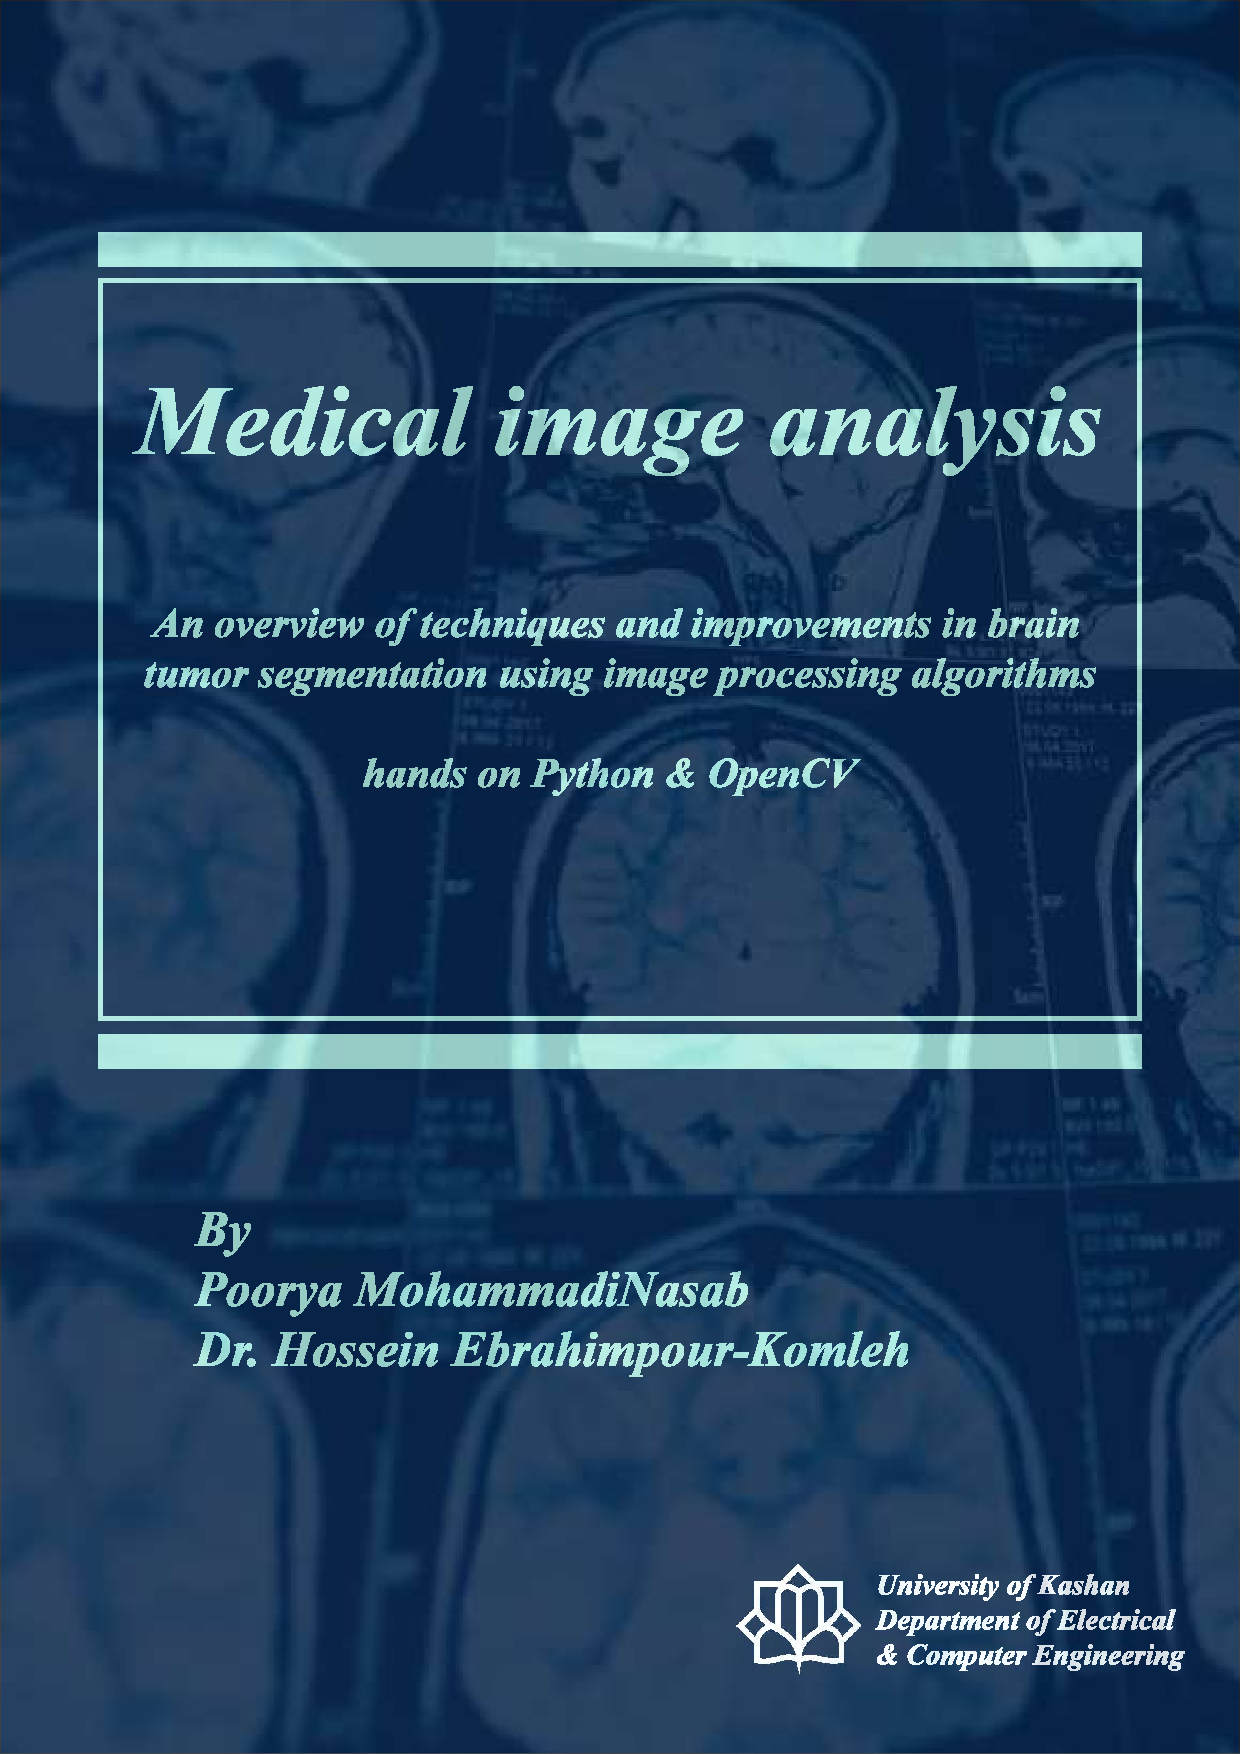
\includepdf[pages=-]{figures/Cover.pdf}

\frontmatter
\maketitle

% acknowledgements chapter
\chapter{Acknowledgements}
\label{sec:acknowledgements}
\let\cleardoublepage\clearpage


\vspace{3cm}

\begin{adjustwidth}{70pt}{70pt}

I would like to thank my teacher, mentor, and thesis supervisor Dr. Hossein Ebrahimpour for his continued guidance and support.
Thanks to the electrical and computer engineering department of university of Kashan for providing me welfare and educational facilities during these years.
And finally, thanks to my parents and numerous friends who endured this long process with me, always offering support and love. 

\end{adjustwidth}

% abstract chapter
\chapter{Abstract}
\label{sec:abstract}
\let\cleardoublepage\clearpage


\vspace{3cm}

\begin{adjustwidth}{70pt}{70pt}
In recent years, the improvement of medical imaging techniques helps doctors to diagnose tumors. Early detection of tumors will increase the chance of treatment and plays an essential role in patient survival. In this thesis project we would like to find how to be an expert in medical image analysis by explaining fundamental concepts like medical imaging modalities and image processing techniques and study recent improvements of segmentation. Also, we provide a tutorial for python programming and OpenCV library to do some practical exercises. At the end of this project we implement a new brain tumor segmentation system based on fuzzy logic and image processing approaches. 

\end{adjustwidth}

\tableofcontents
\mainmatter
%\chapter{Motivation of the Project}
\label{sec:chap1}
% definition of tumor

% chapter 1 added to chapter 2
\chapter{Introduction to Medical Image Analysis}
\label{sec:chap2}

\section{Motivation}
A \textbf{tumor} is an abnormal mass of tissue that forms when cells grow and divide unusually. Tumors are divided into two main categories: benign (not cancer) or malignant (cancer). Benign tumors may grow large but do not invade other parts of the body.  On the other hand, malignant tumors can spread into nearby tissues.

There are different reasons for creating tumors; the first reason is the body tissue near the tumor area. But in some cases, it is brought from other parts of the body. The risk level of tumors depends on four factors: 

\begin{enumerate}
	\item Type of the tumor (benign or malignant)
	\item Size of tumor
	\item Location of tumor
	\item Speed of tumor spread
\end{enumerate}

In recent years, the improvement of medical imaging techniques helps doctors to diagnose tumors. Imaging tests are used to determine the size and location of cancer. Medical imaging is a technique and process to build a picture of the whole human body or a part of it for medical purposes. 

Early detection of tumors will increase the chance of treatment and plays an essential role in patient survival. On the other hand, manual tumor segmentation (by an expert) among a large number of medical images could be hard and time-consuming.  Also, it depends on the experience of the expert who does this segmentation. Therefore, we need a completely automated and precise approach to segment and detect tumors. Recently, using image processing and machine learning methods has become common due to their promising results. 

A thorough analysis of the literature with the keywords ‘brain tumor segmentation’, ‘medical image segmentation machine learning’, and ‘medical image analysis deep learning’ on the Google Scholar search engine is performed in Fig. \ref{fig1}, queried on August 16, 2021. We can observe that the number of papers increases every year from 2013 to 2021, which means multi-modal medical image segmentation using machine learning, and deep learning are obtaining more and more attention in recent years. 

\begin{figure}[h]
	\centering
	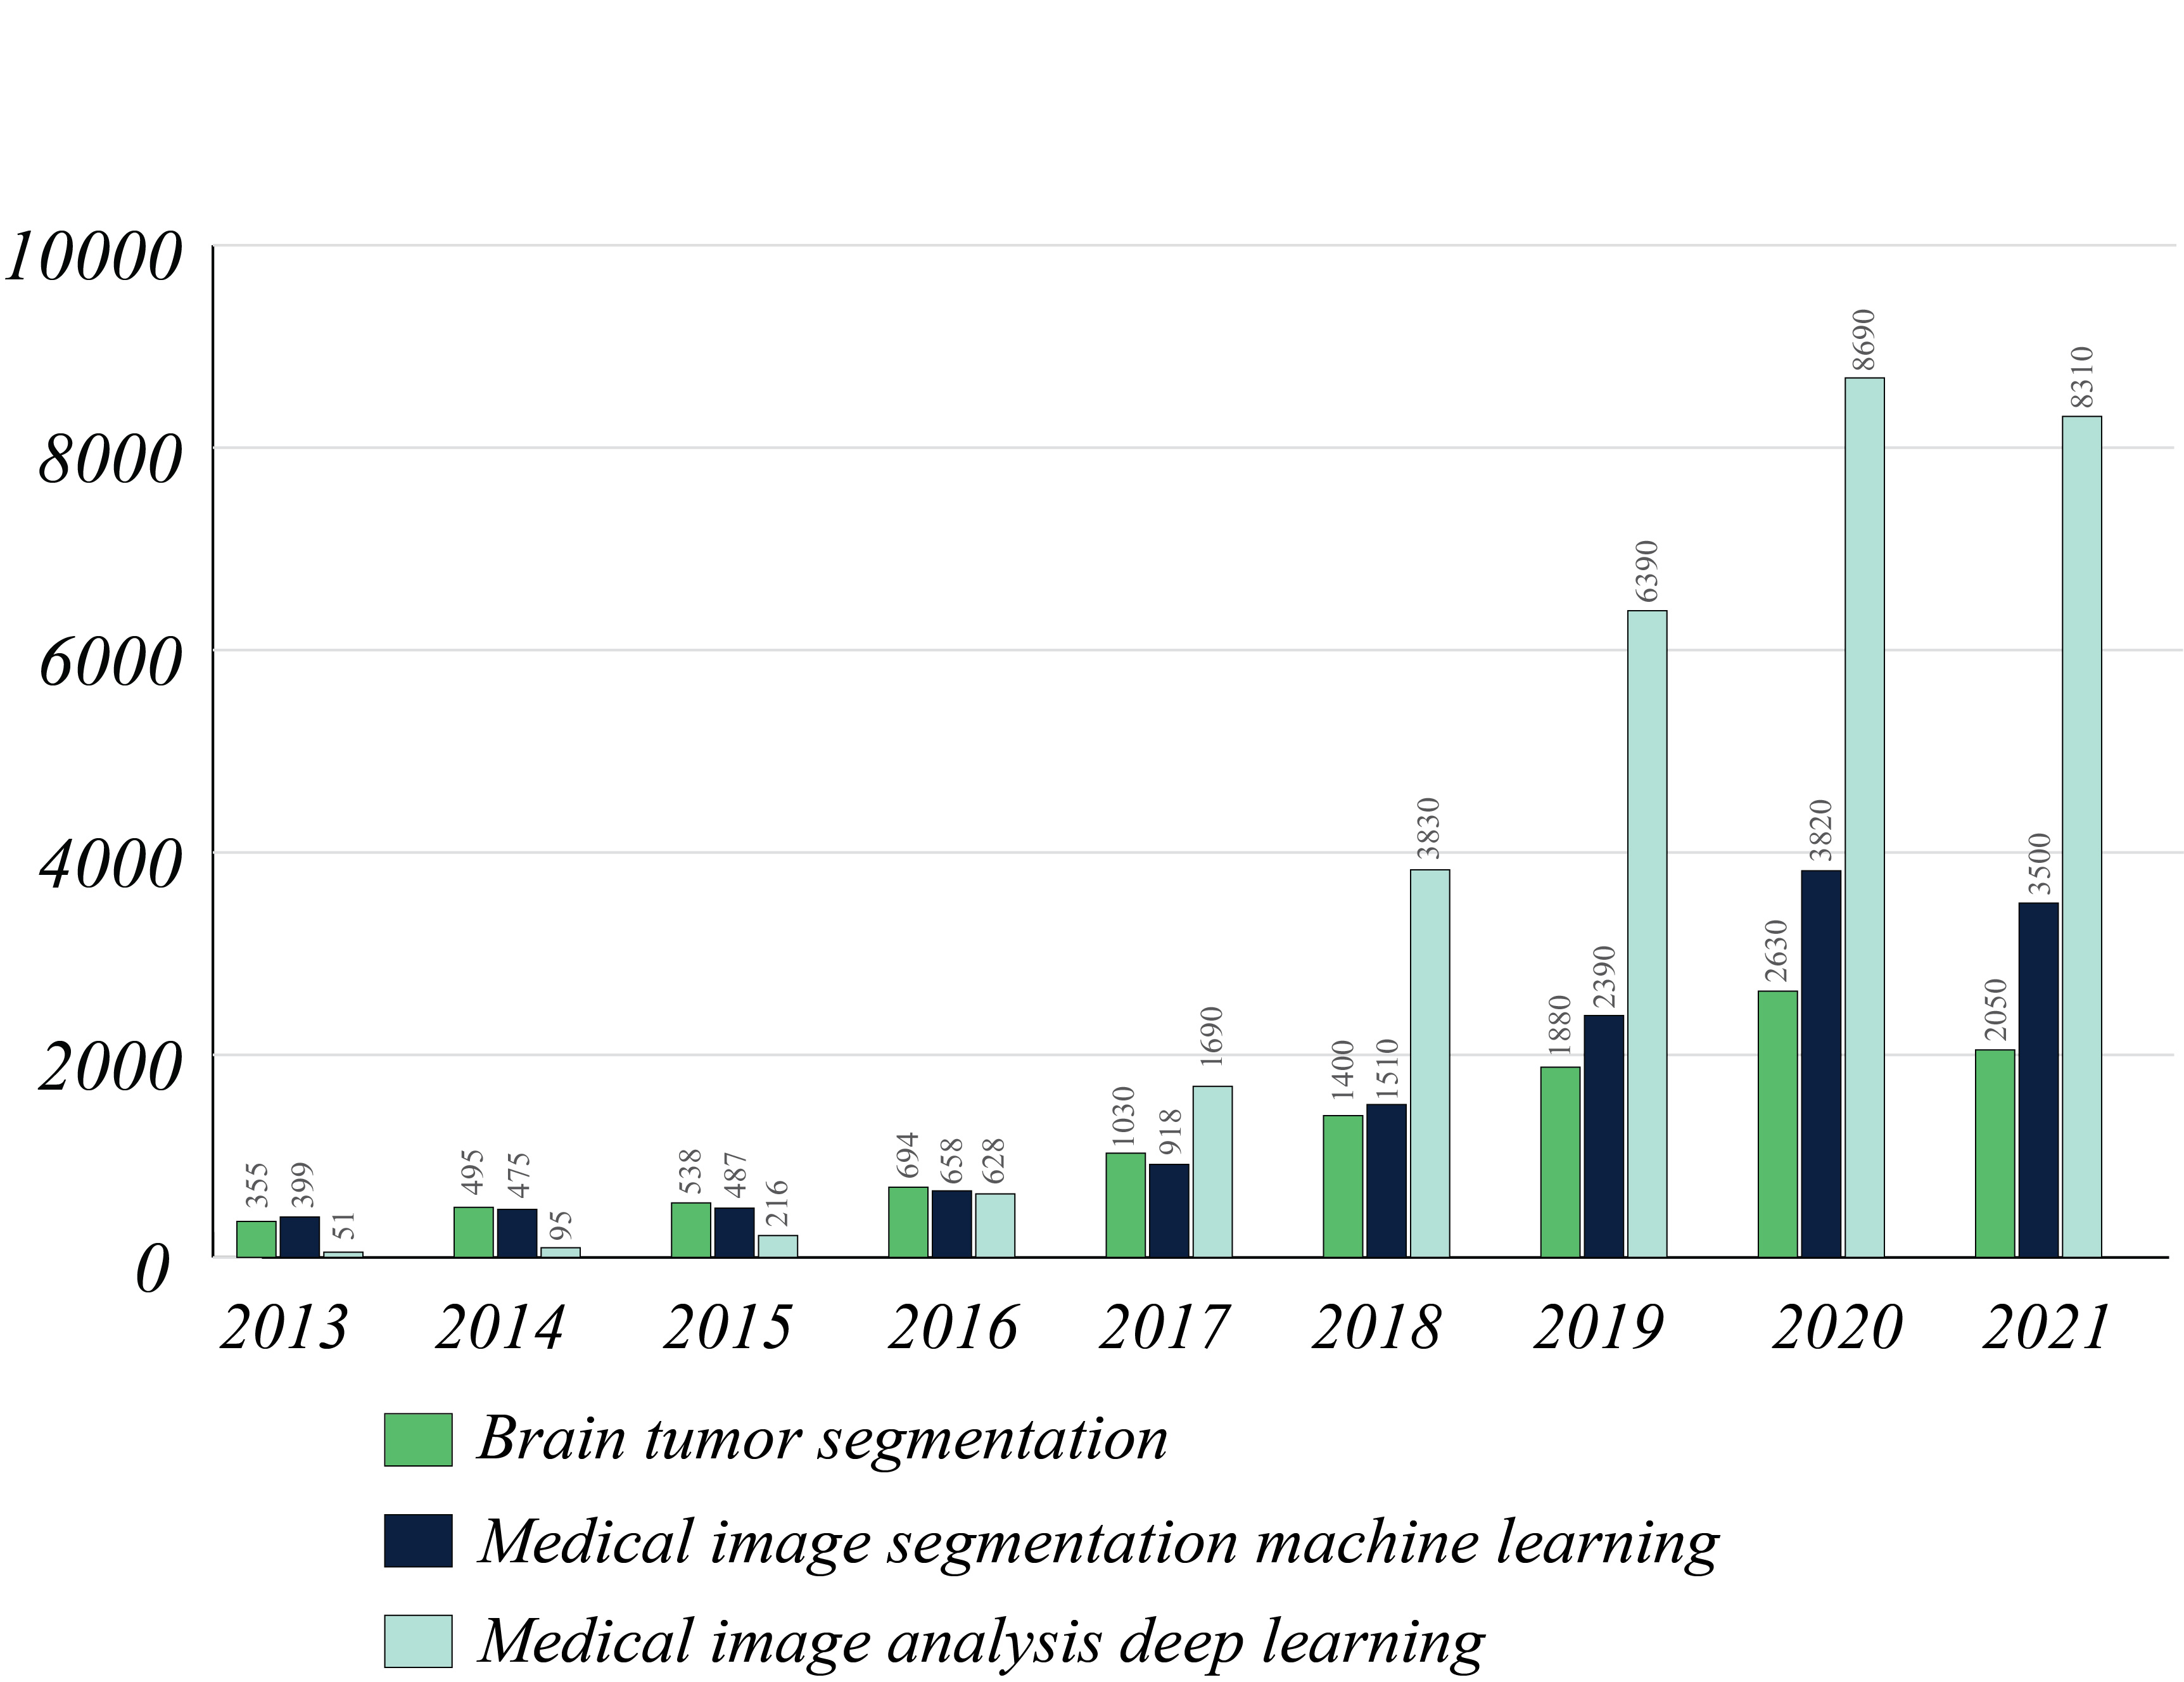
\includegraphics[width=1\columnwidth]{./figures/Fig1.jpg}
	\caption{Keywords search results}
	\label{fig1}
\end{figure}

\section{what is medical image analysis}

In 2020, the whole machine vision market was worth about 12.29 billion dollars, and out of this, 39\% of the total share would be what will be taken down by medical image analysis itself. It will not be focused on hospitals or private health care centers or any particular modality like x-ray or ultrasound. So we can use it in different modalities, clinical indications, and different end-users. Figure \ref{fig2} illustrates the concepts and applications of medical image analysis.

\begin{figure}[h]
	%\resizebox{\linewidth}{!}{
	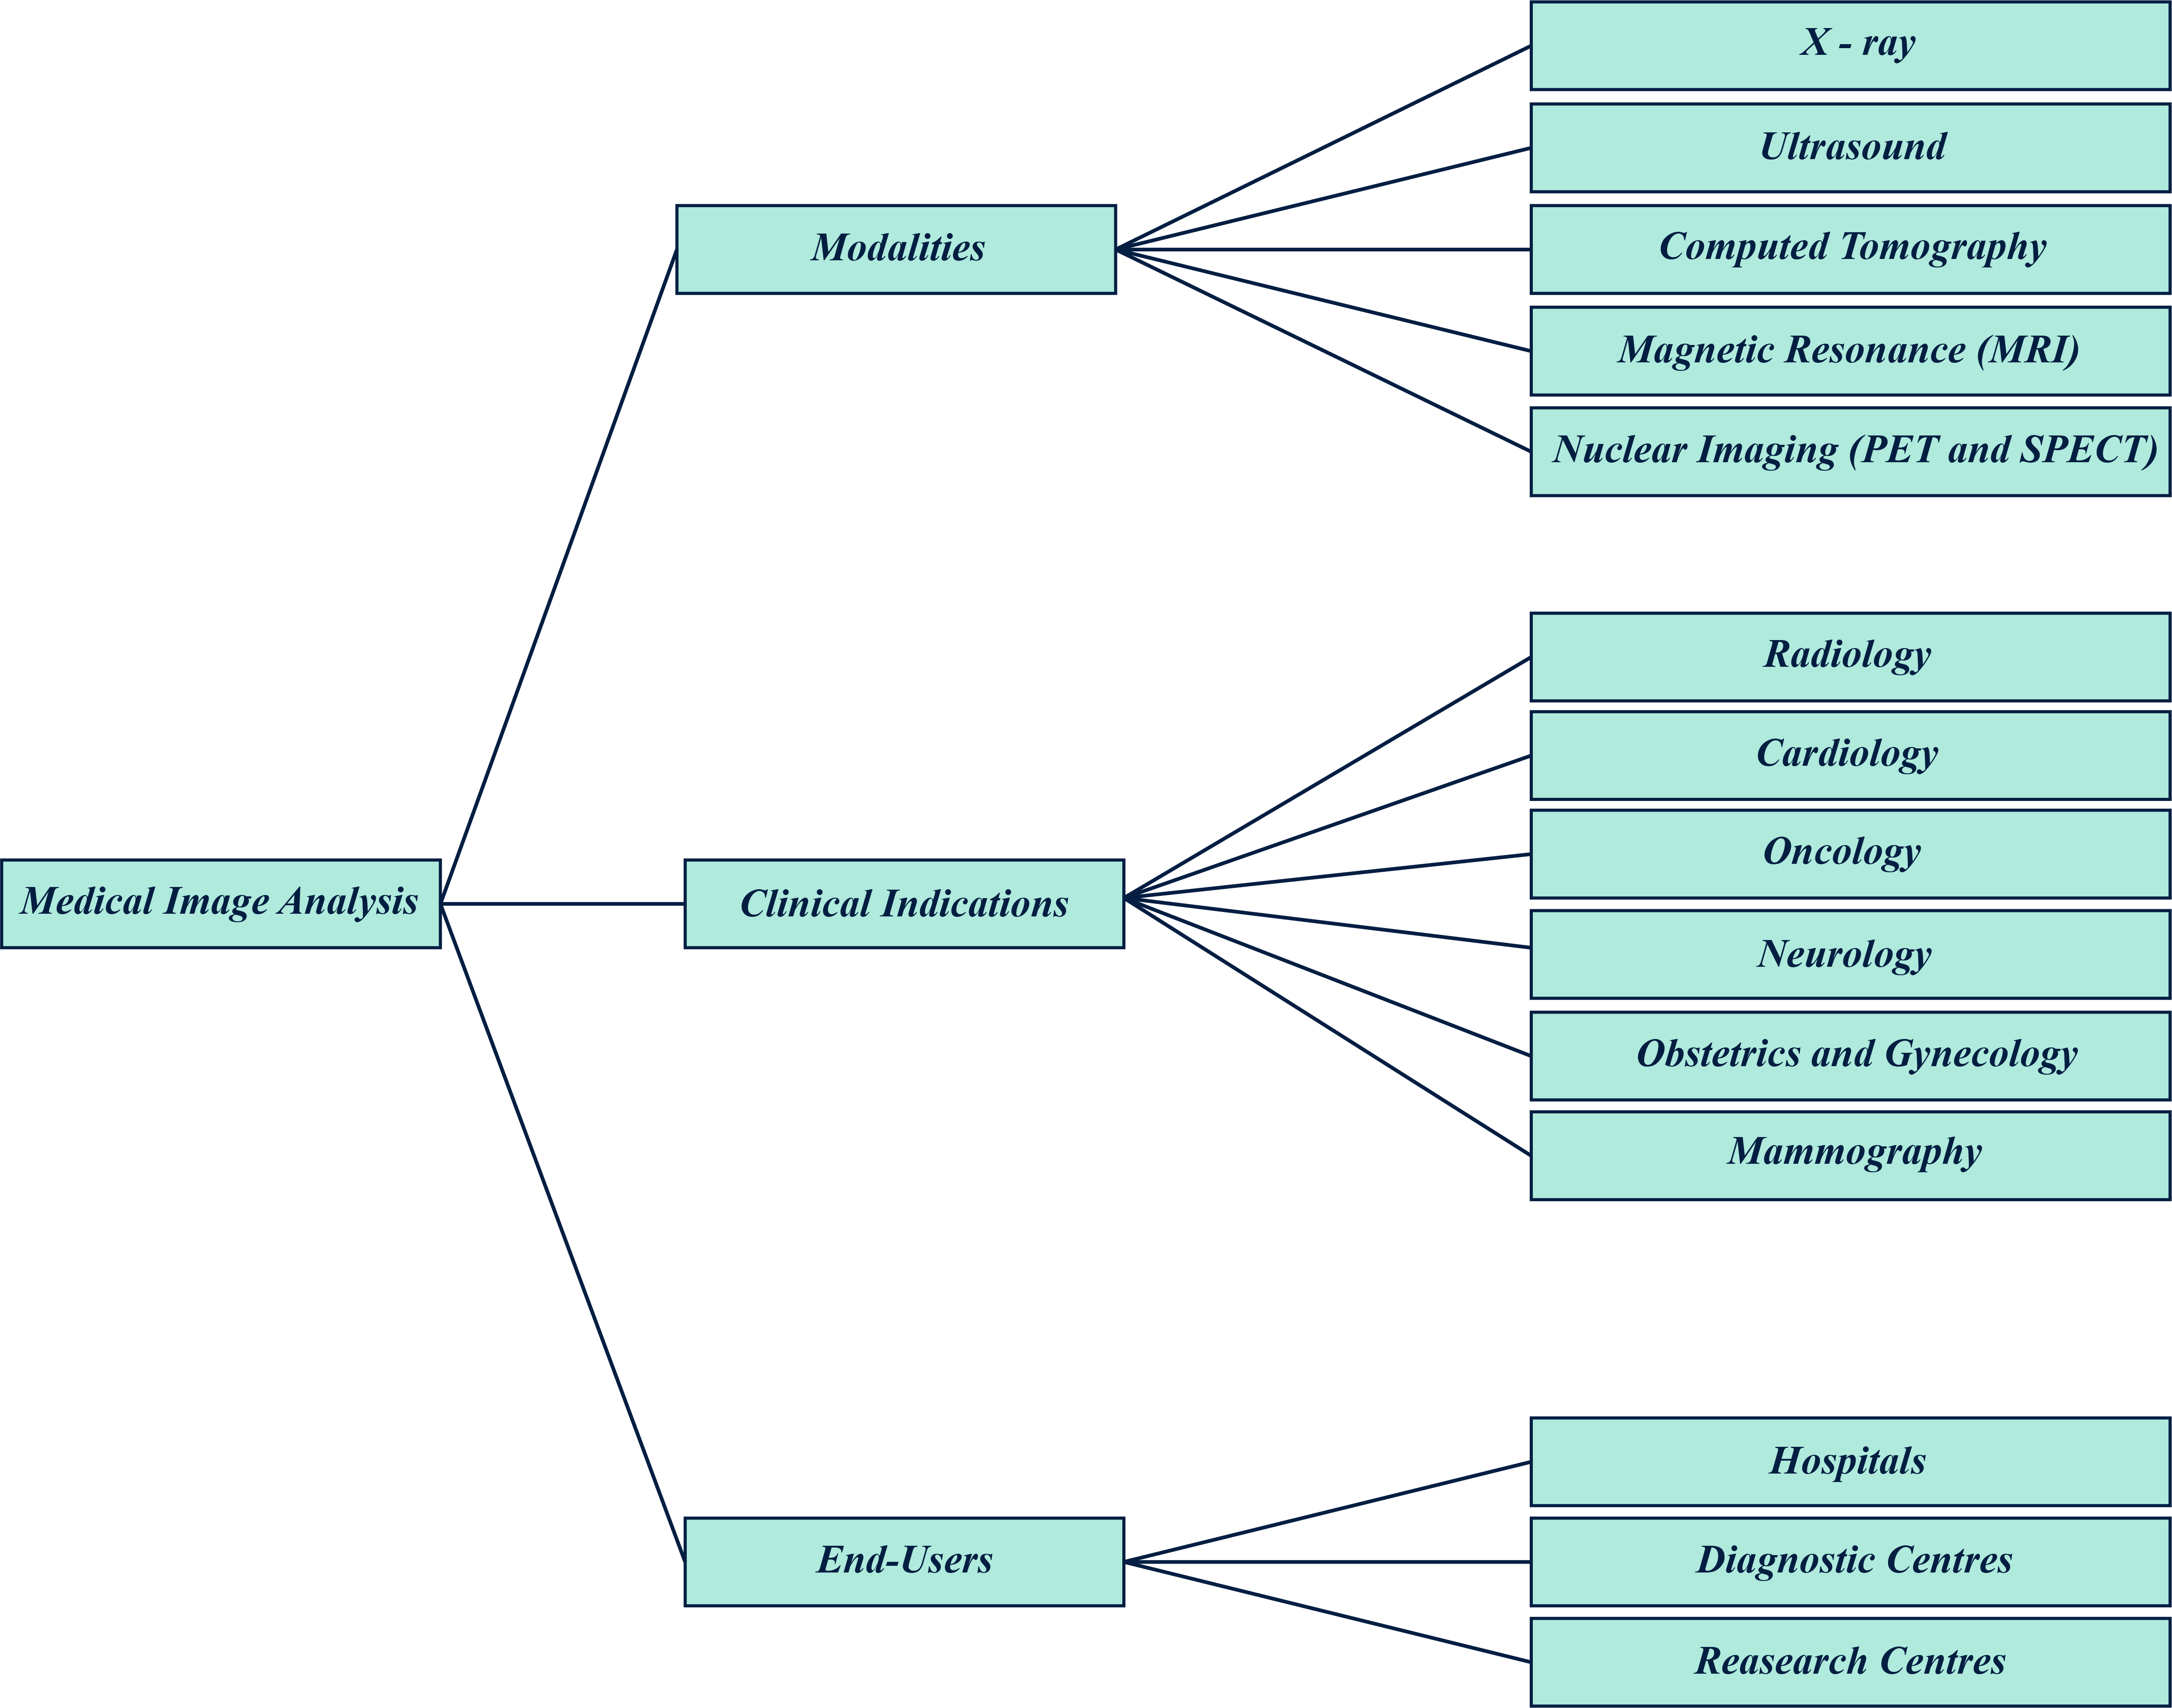
\includegraphics[width=1\columnwidth]{./figures/Fig2.png}
	\caption{Medical image analysis (concepts and applications)}
	\label{fig2}
\end{figure}

\section{roadmap}


If we look into different modalities such as CT, MRI, ultrasound, etc. The critical part is about the organ appearance module and what they mean. In other words, how different organs are going to appear in different modalities. For example, a bone will appear brighter on x-rays, and it would be darker on T1 MR and T2 MR. On the other hand, fatty regions appear brighter on MR and darker on x-rays; fatty areas will appear brighter on ultrasound. A water-filled part that would appear brighter on MR will appear darker on ultrasound.

The second part for understanding medical image processing is to understand the physics part of it. As we mentioned above, different parts of the body have different ways in which they are viewed, and it is where we need to understand tissue energy interactions together. And from there, image formation and statistics of image formation will get vital because we will see a lot of noise and uncertainty. For example, ultrasound is a specular modality that has a lot of jitters and noise around intensities.
On the other hand, MRI will not have that much problem, but it suffers from lower resolution than ultrasound, and when we go into detail understanding of each of this physics and how operating conditions of an instrument affects the total resolution of image formation.

After medical imaging and physics, we would be moving on to image processing and graphics in the third step. Image processing is an essential part of medical image analysis because it contains Denoising, feature segmentation, image segmentation, and feature representation. After that, we got onto a very critical factor called visualization. Also, knowledge of graphics is fundamental. 

Last but not least is machine learning which has grown in recent years. Machine learning includes prediction models and a group of classifiers. We can use various methods to solve a particular problem, such as example-based learning methods or complex reasoning. So to conclude these four main steps of medical image processing, we bring them as Figure \ref{fig3}.

\begin{figure}[h]
	%\resizebox{\linewidth}{!}{
	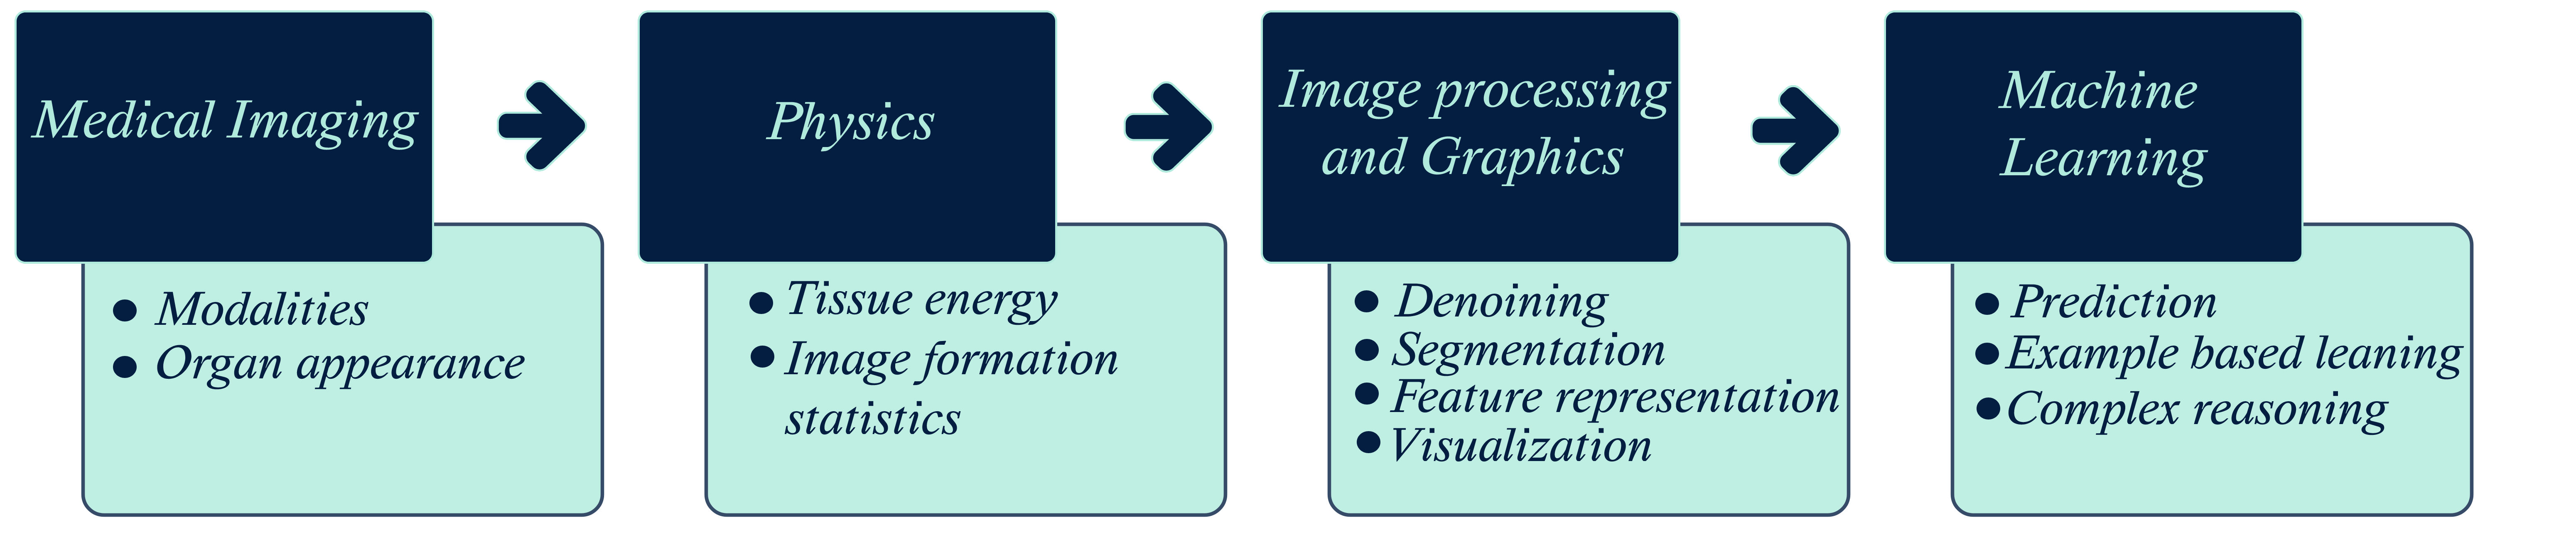
\includegraphics[width=1\columnwidth]{./figures/Fig3.png}
	\caption{Medical image analysis roadmap}
	\label{fig3}
\end{figure}

\section{research and business areas}

Let us look into the main areas of research and business that medical image analysis is concerned. The first one is the range of image modalities which are macro and micro imaging. Macro imaging is the method that the whole body gets imaged together, and obviously, the resolution is much lower, but the penetration depth is much higher. On the other hand, micro imaging has resolution at the microns' level and is used in some modalities like optical coherence, tomography, and histopathology for digital pathology. But, there is a tradeoff for scaling, and it is mesoscopic range imaging.

The second main area is image registration, a classical area for medical image analysis, and it says a patient goes for a CT scan. After six months, he or she does this again but at a different location and different CT machine. The resolutions are different because the patient might have a body change, such as losing some weight. The doctor wants actually to relate to what happened in the last six months. 

Another exciting area is organ localization which is where we need to find out the organ itself. This area uses algorithms to make it much easier for clinicians than wasting a lot of time. Also, As you know, we imaging in 3D, but you see the output on your computer screen or x-ray films which present only 2D pictures. Organ localization tries to use algorithms in 3D and segment them. After organ localization has been over, you can segment out and get the volume information and surface information.

In recent years, the research on visualization using augmented reality has been expanded. This area is related to present how different kinds of fractures can be there on a bone and then try to find out what the bone would look like without any fractures. 

Another interesting field is virtual anatomy, and it comes after we have a complete MR or CT scan of a patient body. The whole anatomy, such as every organ and every tissue or bone, is digitized and segmented using virtual anatomy. In other words, the body is equivalent to a computer-aided design (CAD) model. For example, if a doctor wants to find out internal injuries, specific legions, or diseases within the patient's body, they do not need to scan every x-ray.  

A very critical application in this area is digital angiography which is also called digital subtraction angiography. It is a technique to find out where is a deposition of blood or regularity inflow of blood.  
Despeakling is related to speckle imaging modalities like optical coherence or ultrasonic tomography, where many speckles lead to tediousness. This situation cannot just be Denoising because it would get rid of edges and salient behaviors. 


3D optical microscopy is a 3d model of a neuron image under fluorescence for different layers, segmented and resynthesized by alignment. We can look at the complete 3D model and view how neurons look and how the processes are going over there. This area has a significant role in a field of medicine called precision medicine. 

Digital pathology is the next critical area. With the help of pathology, the pathologist doesn't need to be at the center where the slide comes down. So say there is a collection center that is far from the actual pathologist is located. Transporting a physical slide takes more time and money, but digital pathology solved this problem. 

The last area in this section is computational imaging. Computational imaging is about synthesizing virtual equivalents of different organ types of different pathology types by looking at simple images and simple signals from image modalities. You can see all these areas in Figure \ref{fig4} .


\begin{figure}[htbp]
	%\resizebox{\linewidth}{!}{
	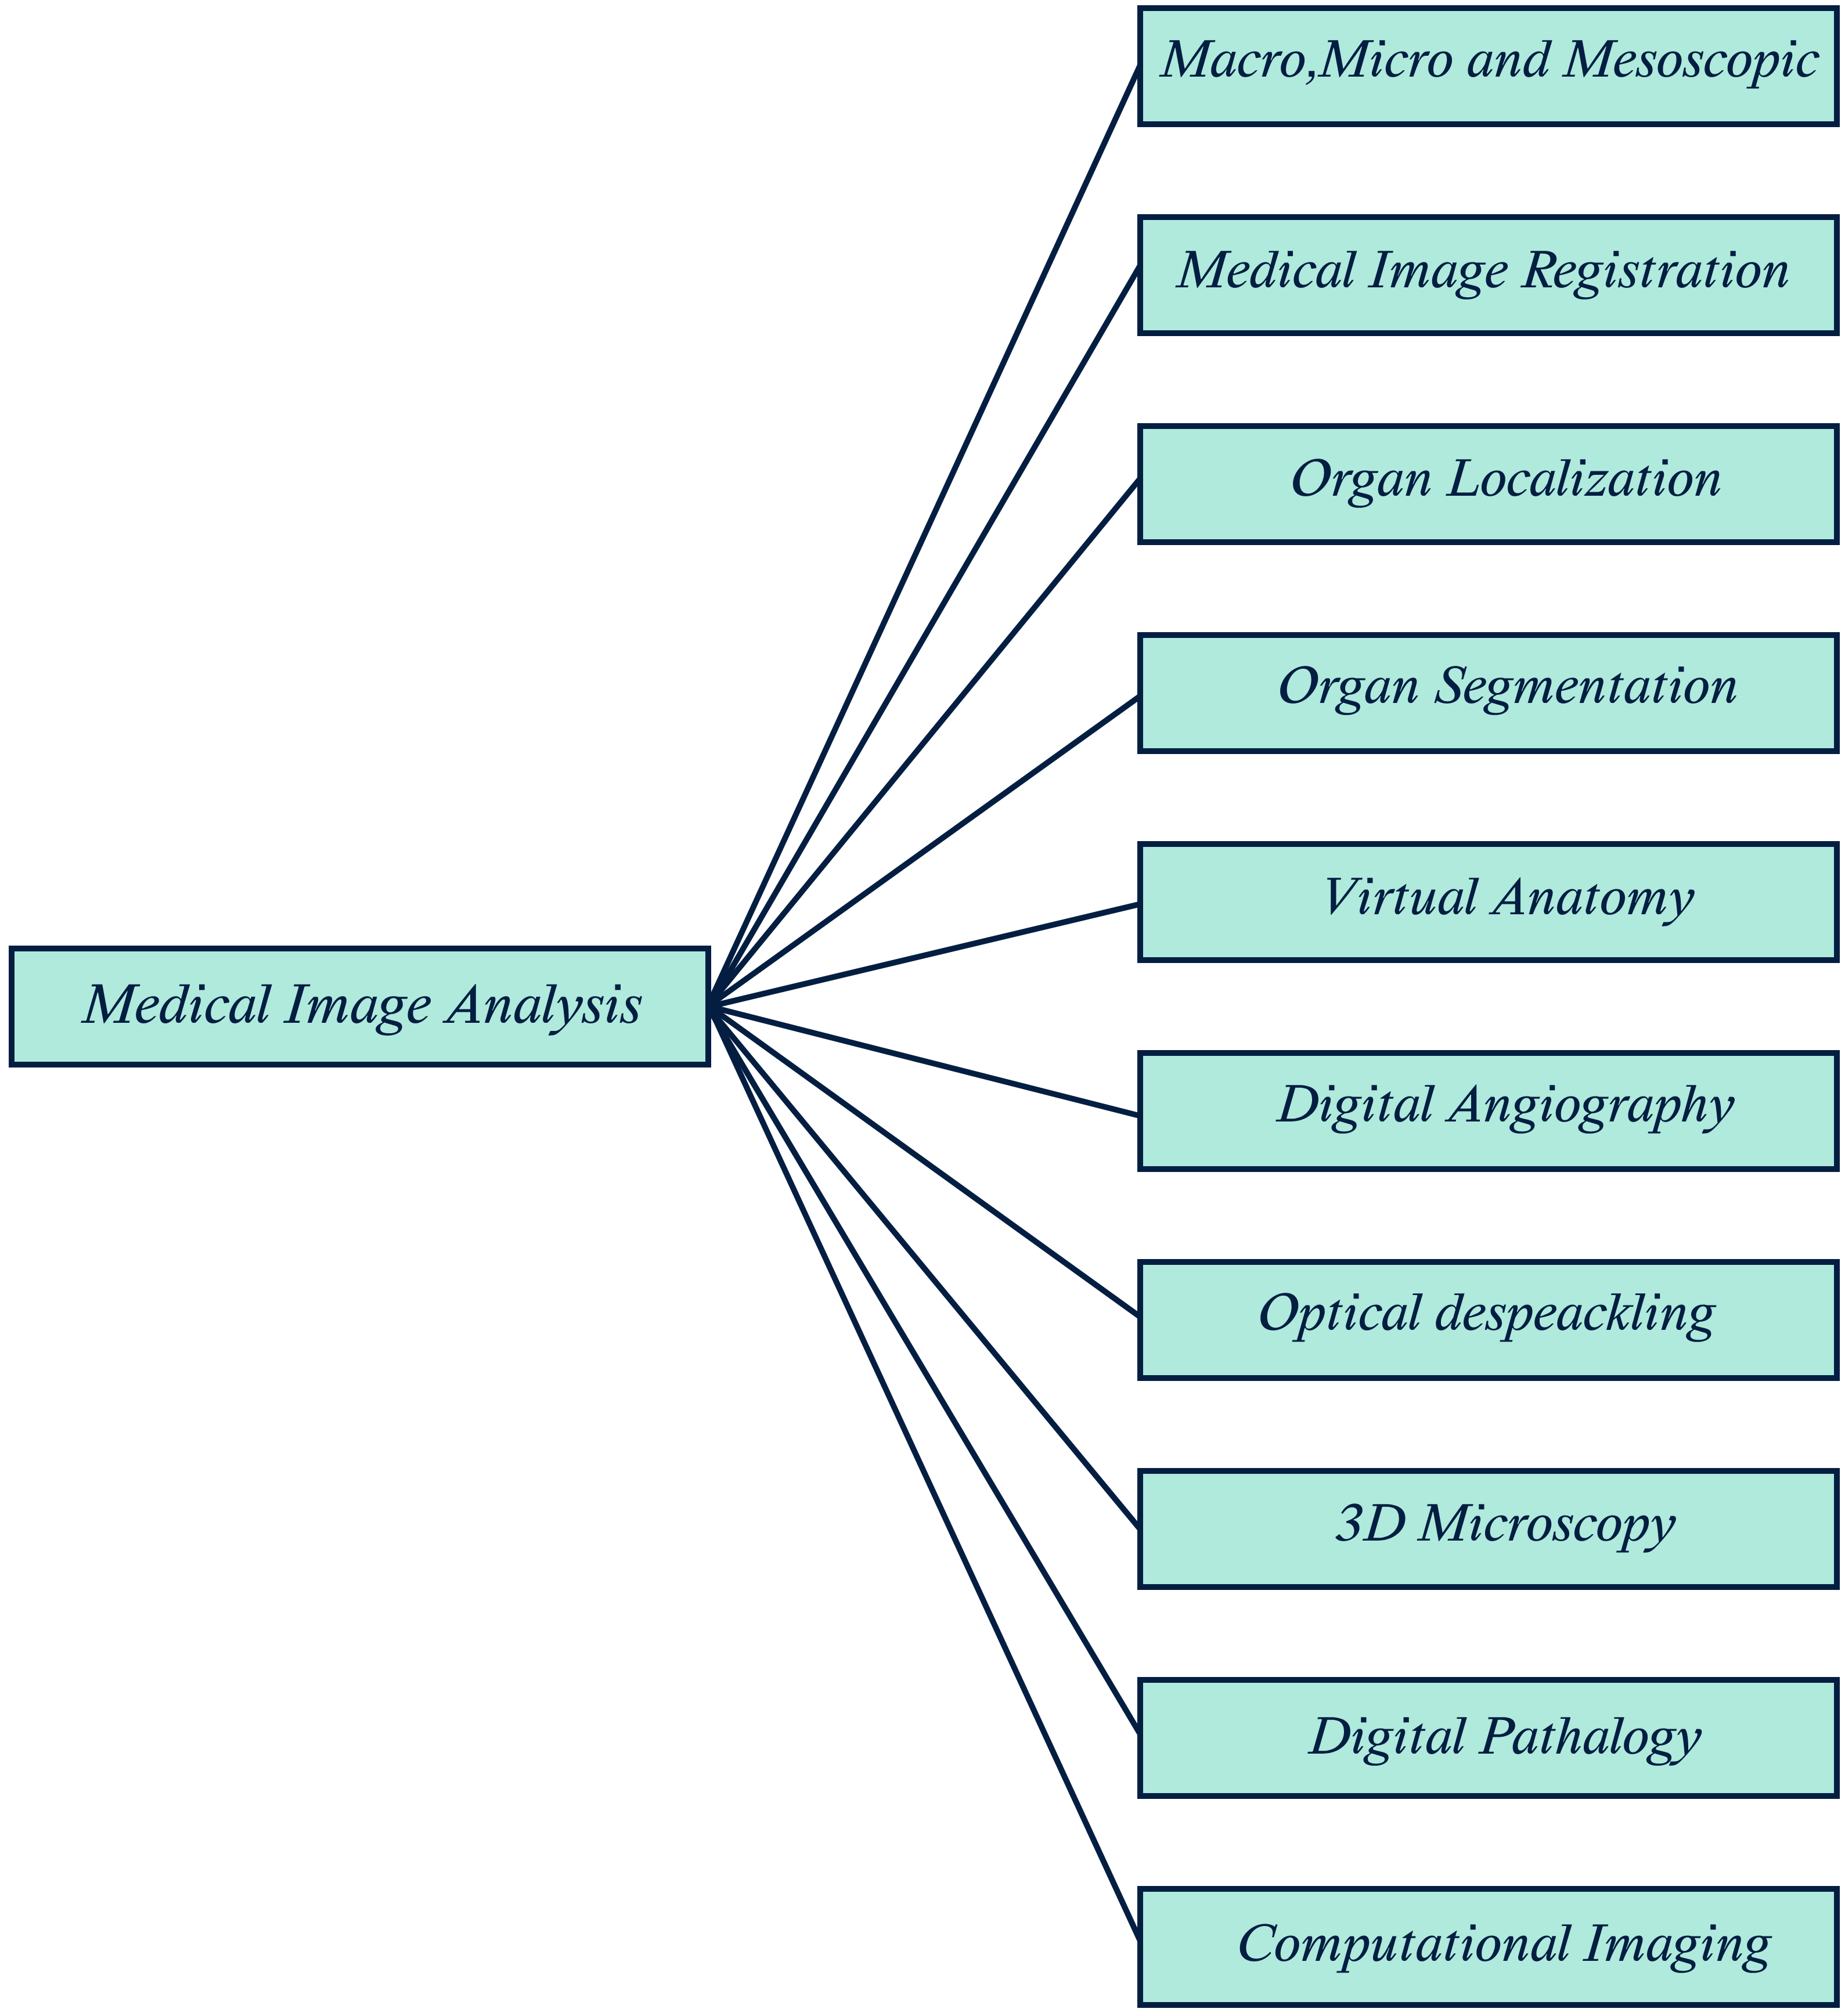
\includegraphics[width=1\columnwidth]{./figures/Fig4.png}
	\caption{Medical image analysis key research(business) areas}
	\label{fig4}
\end{figure}

\section{last 35 years of medical image analysis}
This short review is based on a survey from Duncan and Ayache in January 2000. This era up to 1984 was basically when pattern recognition and analysis were carried on 2D images. Between 1985 and 1991, knowledge-based approaches started, and in that period, we had rule-based analysis and rule-based influencing. From 1992 to 1998, a lot of 3D imaging started into play, and contribution was about storing a more significant amount of data. Silicon fab processes improved process time. For example, nowadays, the whole human body CT could be processed in a couple of minutes, but it took about 24 hours in the past. 

1999 to 2010 was the era of Shallow Reasoning with machine learning, and that is when again you have a lot of computing power. The final period, 2010 until now, is real booming in the field of how neural networks and deep learning was coming up and that is when complex reasoning started. A lot of approaches was developed in this period.

\begin{figure}[htbp]
	%\resizebox{\linewidth}{!}{
	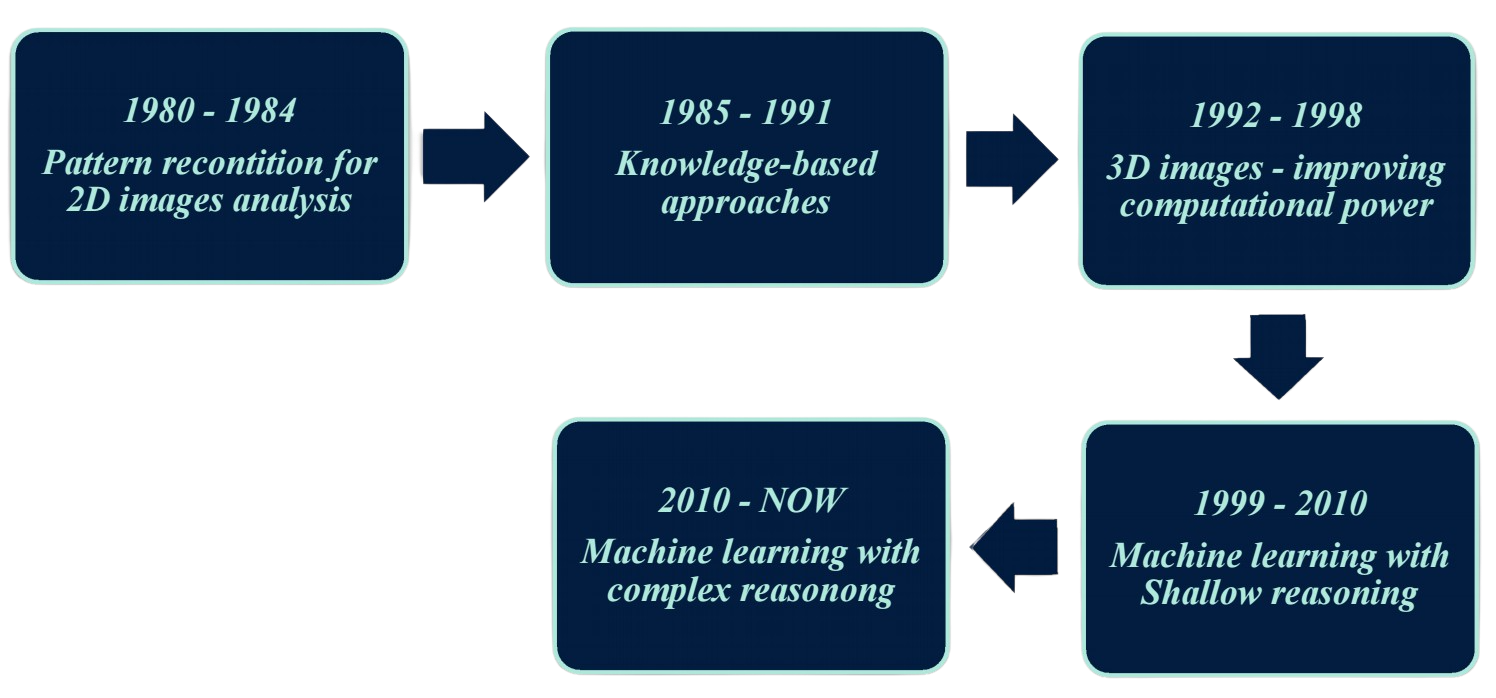
\includegraphics[width=1\columnwidth]{./figures/Fig5.png}
	\caption{Medical image analysis key research(business) areas}
	\label{fig5}
\end{figure}


\section{challenges}

One of the most important challenges for medical image processing is automated detection and classification of breast cancer, and it also called as CAMELYON2017. The next challenge is about prostate lesions segmentation. Then you have the very famous sclerosis from brain MR. The next interesting problem called as M2CAI and this is where we look into interventional videos about surgeries. In other words, M2CAI is modeling and monitoring of computer assisted intervention. The final challenge is ultrasound nerve segmentation.
\chapter{Medical imaging techniques}
\label{sec:chap3}

\section{X-Ray \& CT Imaging}
X-ray is one of the early modules introduced by Wilhelm Rontgen. With this modality, we could look within the body without having to cut the body. Another modality that goes along with x-ray is computed tomography (CT). Computed tomography allows you to look into the 3D projection of every single part of the body and create visual anatomy of the body.

The first part is on x-ray generations and how it works. We have something called an \textbf{x-ray tube}, and this is the source of generated x-ray. It is not an optical photon, i.e., unlike LED lights or tungsten filament lamps where you pass electricity, and it is directly generated; in other words, it is an indirect process.

In this tube, there is a cathode that is heated up, and then it has many electrons around it. On the other side, an anode is a positively charged surface, and it would be a striking anode. In the next step, x-rays will be emitting. Figure \ref{fig6} illustrates this process.  

\begin{figure}[h]
	\centering
	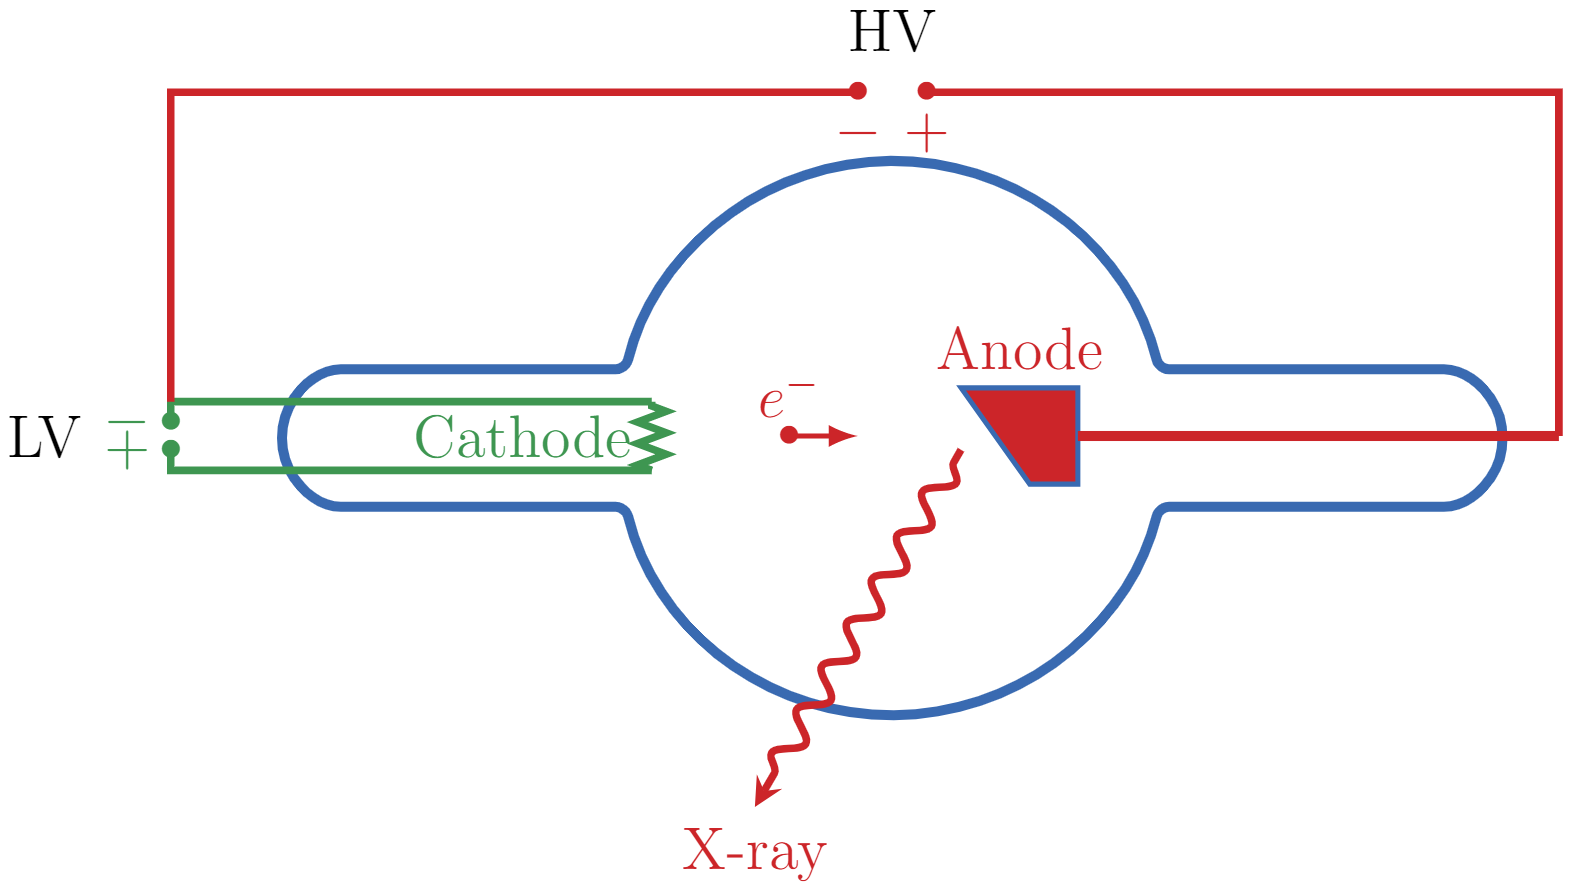
\includegraphics[width=0.7\columnwidth]{./figures/Fig6.png}
	\caption{X-ray generation process}
	\label{fig6}
\end{figure}

For more clarification, we focus on reflected x-rays. As you can see in figure \ref{fig7}, there is a 45 degrees inclination angle. For example, if you have an object at 45 degrees, you will get a reflection, and the angle between this reflection and the incidence ray is 90 degrees. With this method, you put an object and get a magnified view of it on a film.

\begin{figure}[htbp]
	%\resizebox{\linewidth}{!}{
	\centering 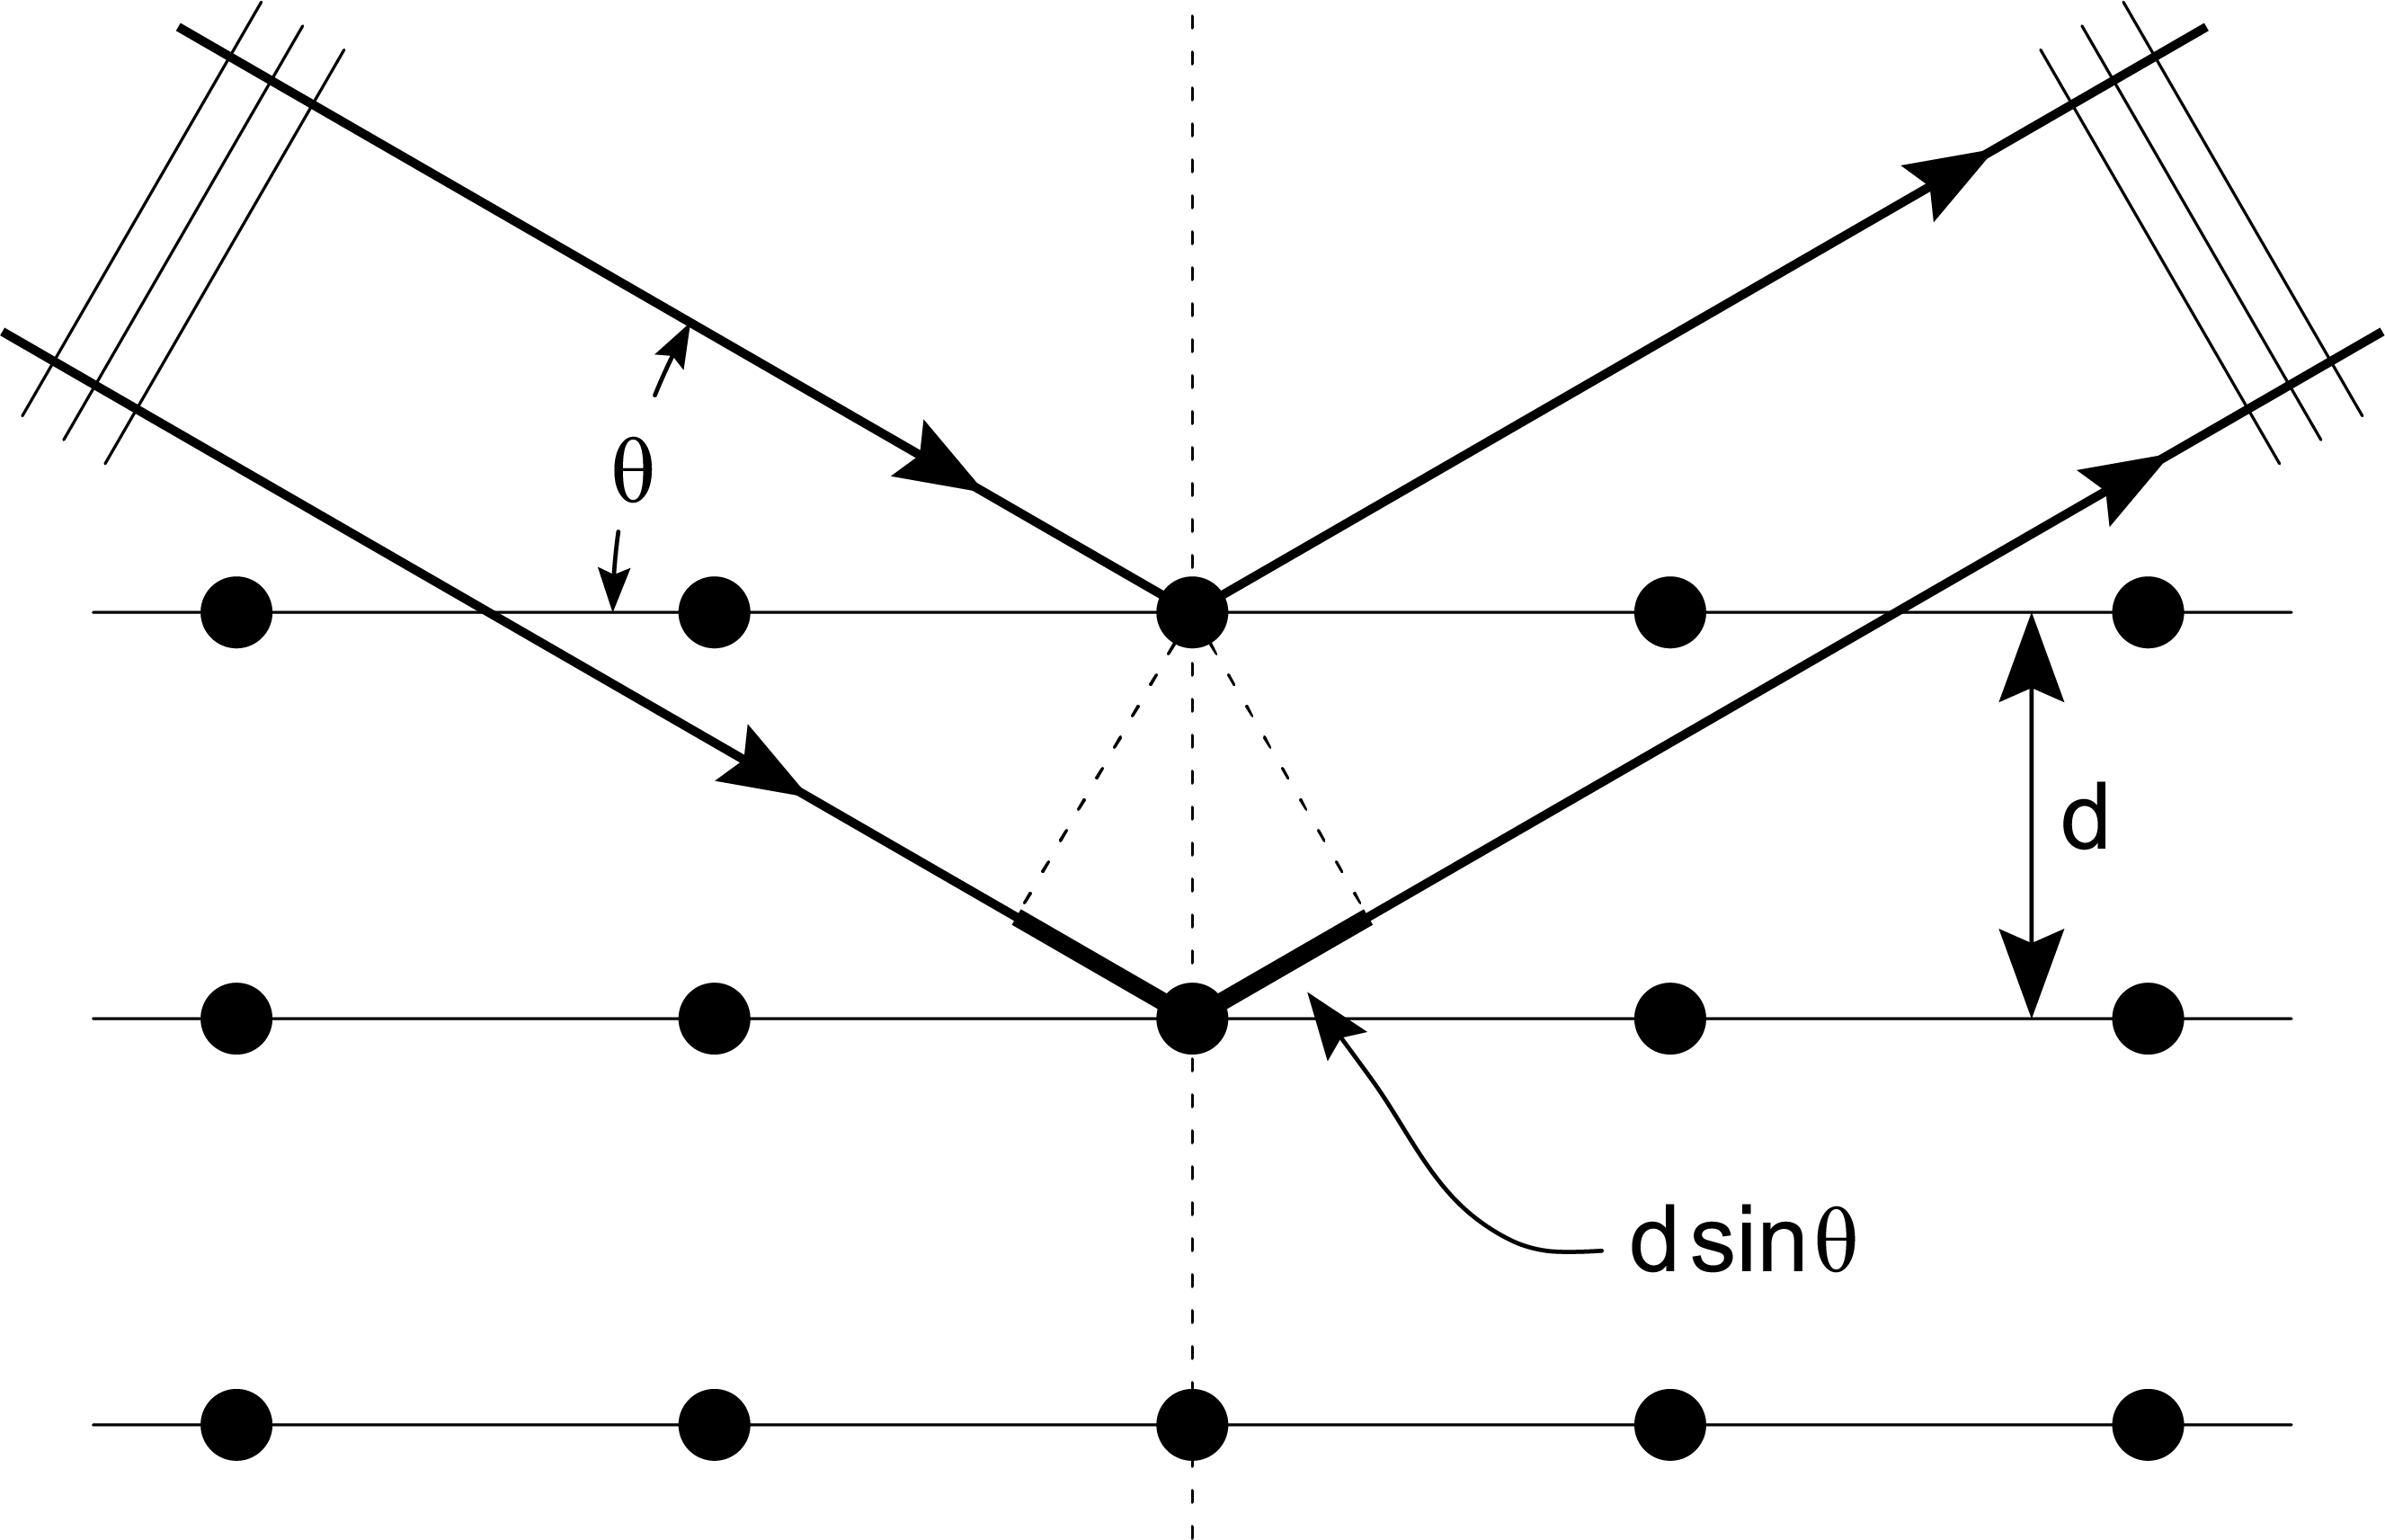
\includegraphics[width=0.7\columnwidth]{./figures/Fig7.png}
	\caption{The process of generation x-ray in more details}
	\label{fig7}
\end{figure}

The next modality is Computed Tomography, and we want to find how to acquire the images using this method. In this method, several detectors have been used, not a single one. The best way is to set an array of sensors, and each has a different line equation, to being solved out when you get the full projection. After that, you need to rotate this pair of the detector array. It keeps on rotating, and you will get multiple projections, so you can backtrack and reconstruct your whole object. Also, it is called CT reconstruction. 

In the final step, we want to find out what is a CT machine looks like. The human body is divided into three planes(x, y, and z-axis); it is three orthogonal planes in medical images. The first plane is called Coronal, which crosses from your left-hand side to the right-hand side and moves the coronal plane from front to back and vice versa. The next one is the Sagittal plane that divides your body into left and right parts, and it can moves from left to right or reverse. Finally, the other plane is called as Axial plane. This plane divides your body into top and lower parts. Figure \ref{fig8} shows a CT machine structure.

\begin{figure}[htbp]
	%\resizebox{\linewidth}{!}{
	\centering 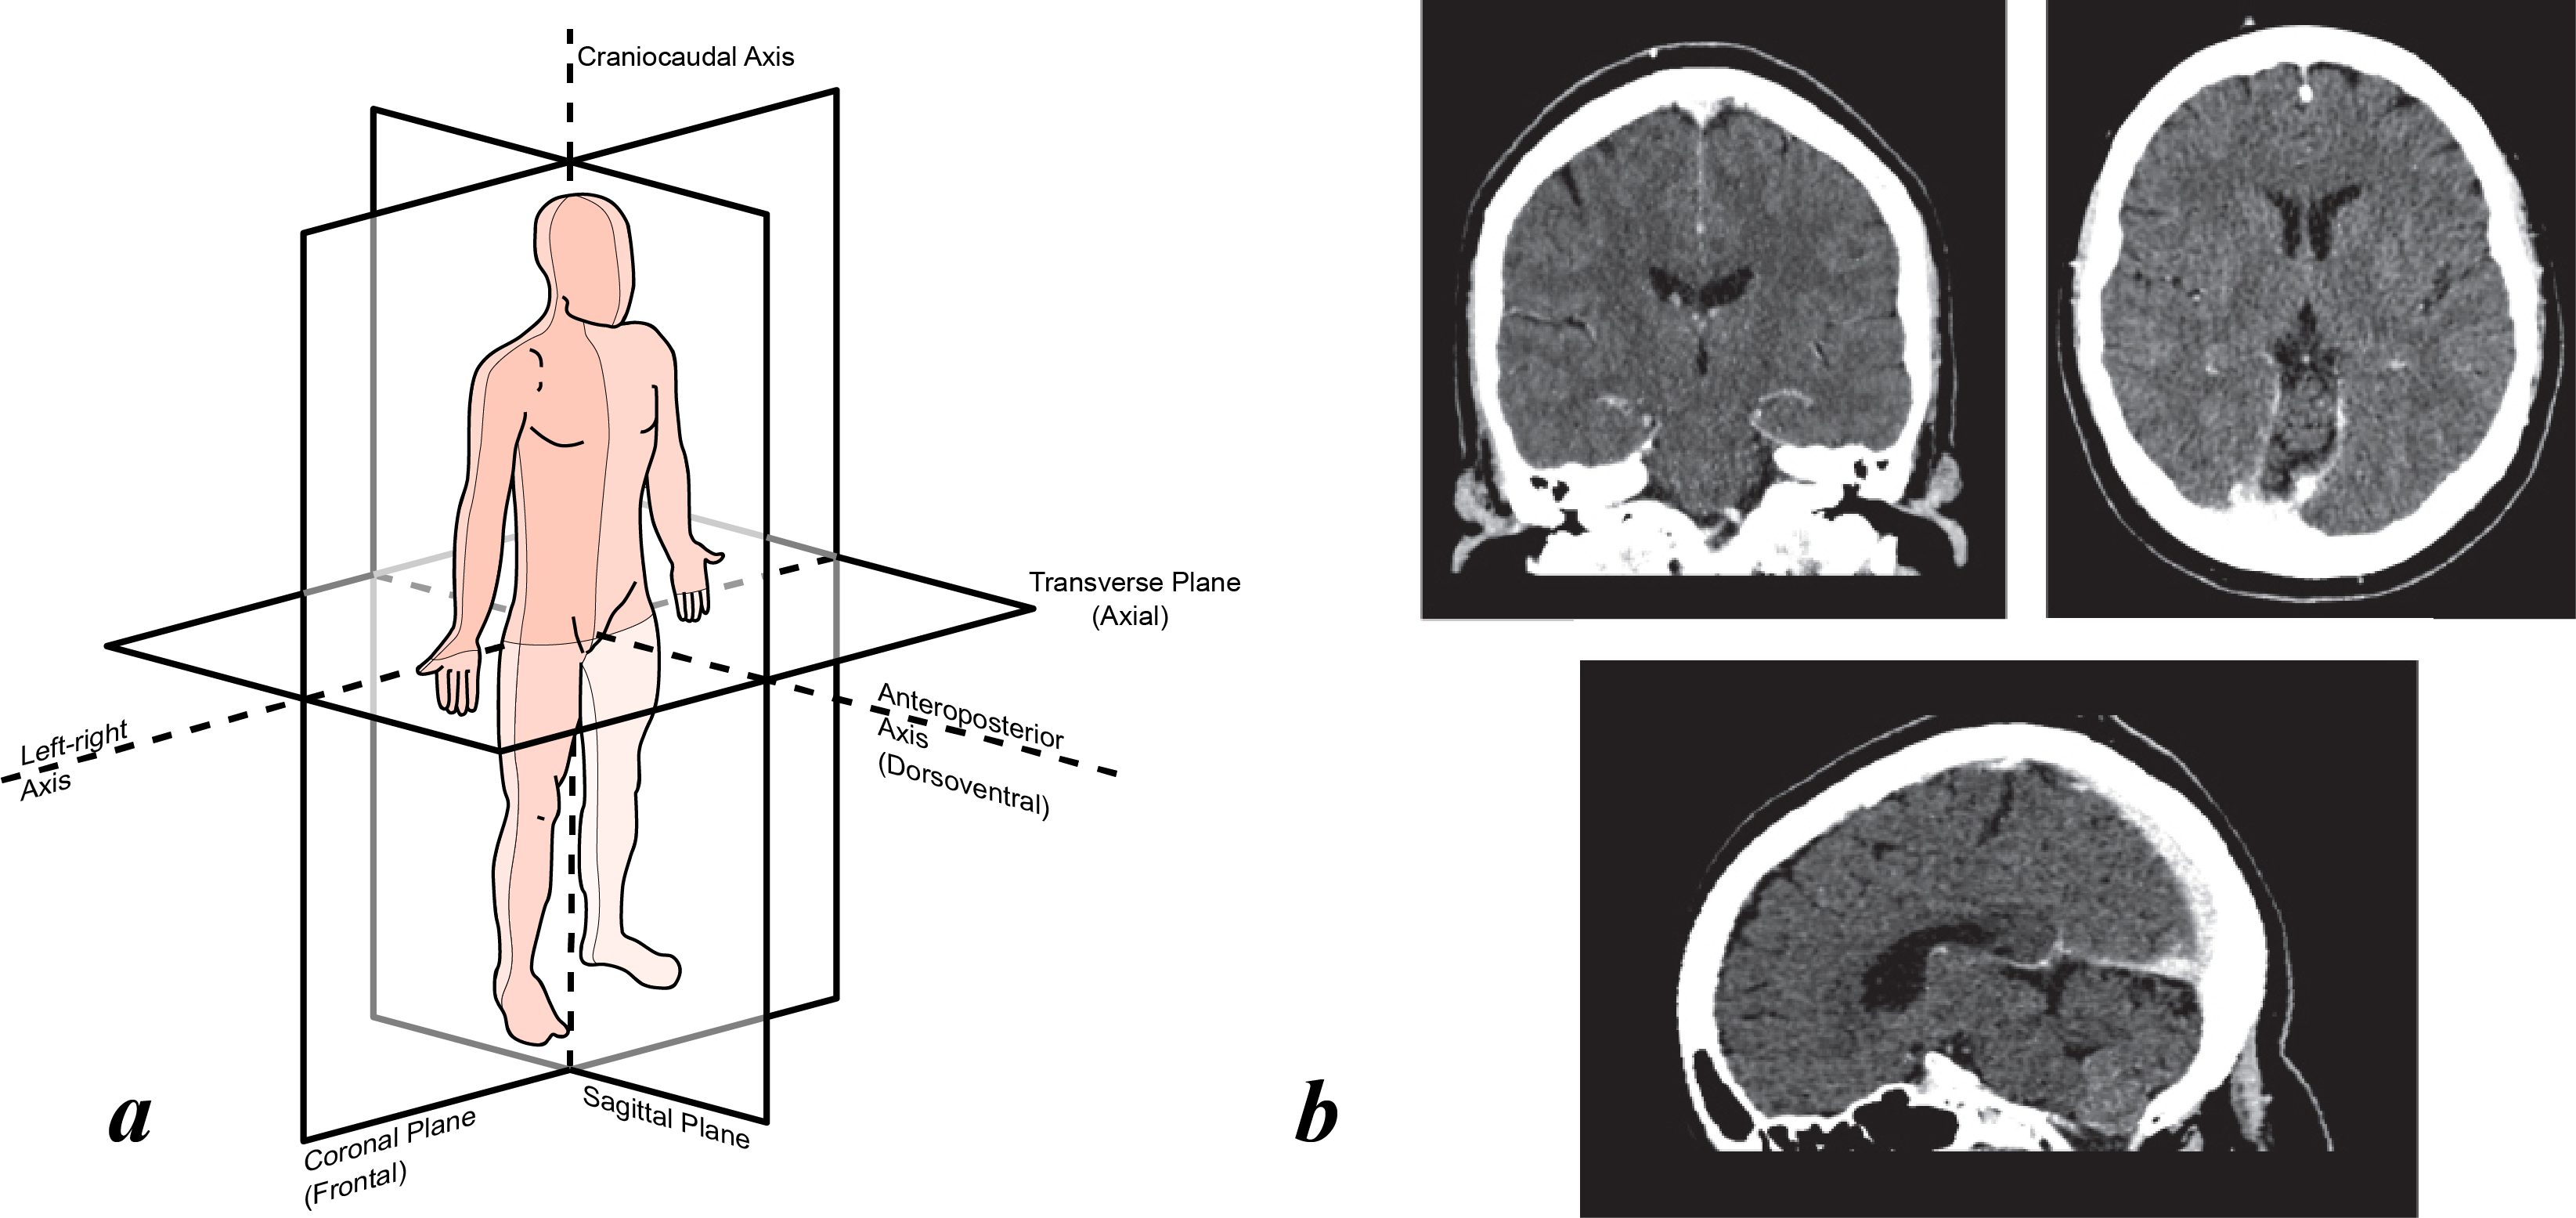
\includegraphics[width=0.85\columnwidth]{./figures/Fig8.png}
	\caption{(a) Diagram of the axial, coronal and sagittal planes. (b) Corresponding CT images of a normal brain.}
	\label{fig8}
\end{figure}


\section{Magnetic Resonance Imaging (MRI)}

The human body is made of multiple small magnets just because of the amount of water drank. This is the base of a concept known as nuclear magnetic resonance. Every single atom has a balanced ratio which is called the gyromagnetic ratio. The first part of MRI is the Spin-Echo concept. If we want to align something from a lower energy state to a higher energy state, we must provide extra energies. When we reduce the energy level, all the protons went down to a higher energy configuration. In other words, they are opposite to magnetic fields.

After some time, due to thermal motion, protons will lose some energy to other atoms. Once they keep on losing energy, they are eventually going to fall to a particular plane. Then some of them will go opposite each other, which means that the net magnetic field is 0. There are some different magnetic field directions. One of them is longitudinal; another one is traverse which is along the opposite direction. Figure \ref{fig9} illustrates these directions.

\begin{figure}[htbp]
	%\resizebox{\linewidth}{!}{
	\centering 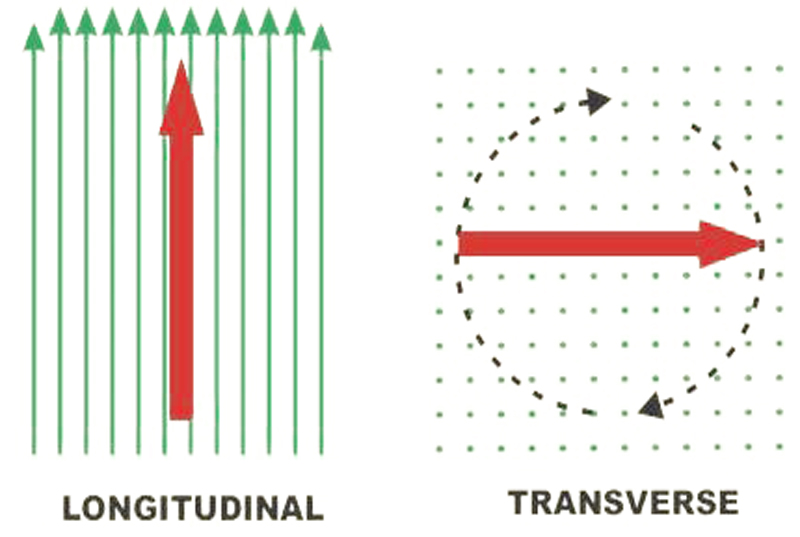
\includegraphics[width=0.55\columnwidth]{./figures/Fig9.jpg}
	\caption{Different magnetic directions}
	\label{fig9}
\end{figure}

Let’s look at different materials and their T1 and T2 relaxation time and as it shown in table \ref{tab1} the highest values are for Cerebrospinal fluids. Another interesting fact is if T1 is increasing, then T2 also is increasing. T1 is higher than fat, whereas T2 is lower than fat. Also, for muscles, T1 is higher than liver although T2 is higher than Liver but is it lower than fat. The first modality is called T1 weighed image and the second one is known as T2 weighed image.

\begin{table}[h]
	\centering
	\caption{Spin relaxation time}
	\label{tab1}
	\renewcommand{\arraystretch}{1.2}
	\begin{tabular}{|c|c|c|}
		\hline
		\textbf{Tissue}              & \textbf{T1(ms)} & \textbf{T2(ms)} \\ \hline
		Fat                 & 260             & 80              \\ \hline
		Liver               & 550             & 40              \\ \hline
		Muscle             & 870             & 45              \\ \hline
		White matter        & 780             & 90              \\ \hline
		Gray matter         & 900             & 100             \\ \hline
		Cerebrospinal fluid & 2400            & 160             \\ \hline
	\end{tabular}
\end{table}


In table \ref{tab1}, those regions with a much higher T1 relaxation time have much higher energy, respectively. If we have an MRI of a brain (Figure \ref{fig10}), it is made out of many fats. In the T1 modality, the fat regions in the brain are shown in white color, while in the T2 modality, it is a gray matter. Also, the correspondences between T1 and T2, white matter, and gray matter appear opposite to each other, and it is because of the relation between these two modalities.

\begin{figure}[htbp]
	%\resizebox{\linewidth}{!}{
	\centering 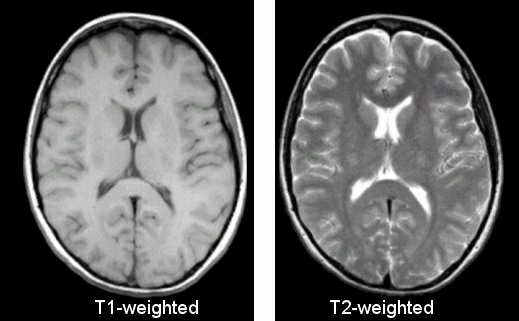
\includegraphics[width=0.5\columnwidth]{./figures/Fig10.jpg}
	\caption{T1 and T2 modalities}
	\label{fig10}
\end{figure}

The primary role of engineering comes into play when we want to apply a trick in MRI. Instead of exposing the whole body to a constant magnetic field, we create a gradient. For example, somewhere around the head, the magnetic field is about 1.5 tesla, and around the legs, it will become about 0.5 tesla. After applying this technique, we can divide the body into different slices, and each piece will have a different frequency.

Table \ref{tab2} is a quick reference for different matters in the body in T1 and T2 modalities. For example, T1 and T2 weighted images for bones or bonny-like structures (including calcifications) have an external signal. It is contrary to CT images; i.e., in CT images, bones were shown as brighter structures.

\begin{table}[htbp]
	\centering
	\caption{Comparison is made on the signal of muscles }
	\label{tab2}
	\renewcommand{\arraystretch}{1.2}
	\begin{tabular}{|c|c|c|}
		\hline
		\textbf{Tissue}            & \textbf{T1 weighted} & \textbf{T2 weighted} \\ \hline
		Bone cortex, calcification & Very low signal      & Very low signal      \\ \hline
		Bone Marrow                & High signal          & High signal          \\ \hline
		Cartilage                  & Iso signal           & Slightly low signal  \\ \hline
		Joint effusion             & Iso signal           & High signal          \\ \hline
		Acute hemorrhage           & Low to iso signal    & Low to iso signal    \\ \hline
		Subacute hemorrhage        & High signal          & High signal          \\ \hline
		Hemosiderin                & Very low signal      & Very low signal      \\ \hline
		Fat                        & High signal          & High signal          \\ \hline
	\end{tabular}
\end{table}


\section{Ultrasound Imaging}

Ultrasound is an exciting imaging modality. The prefix ultra means it is above our standard audible limit. Human ears can hear with frequencies from 20 hertz to 20-kilo hertz. In this imaging method, you have a transducer placed in exact contact on the surface; it shouldn’t have an air gap. The transducer emits a tiny bit pulse known as acoustic pulse. Actually, in ultrasound imaging, we probe waves in a fixed period and then draw the contour of all the points. It is like we throw a stone in water, and then we see circular waves around it. Figure \ref{fig11} illustrates the ultrasound mechanism.

\begin{figure}[htbp]
	%\resizebox{\linewidth}{!}{
	\centering 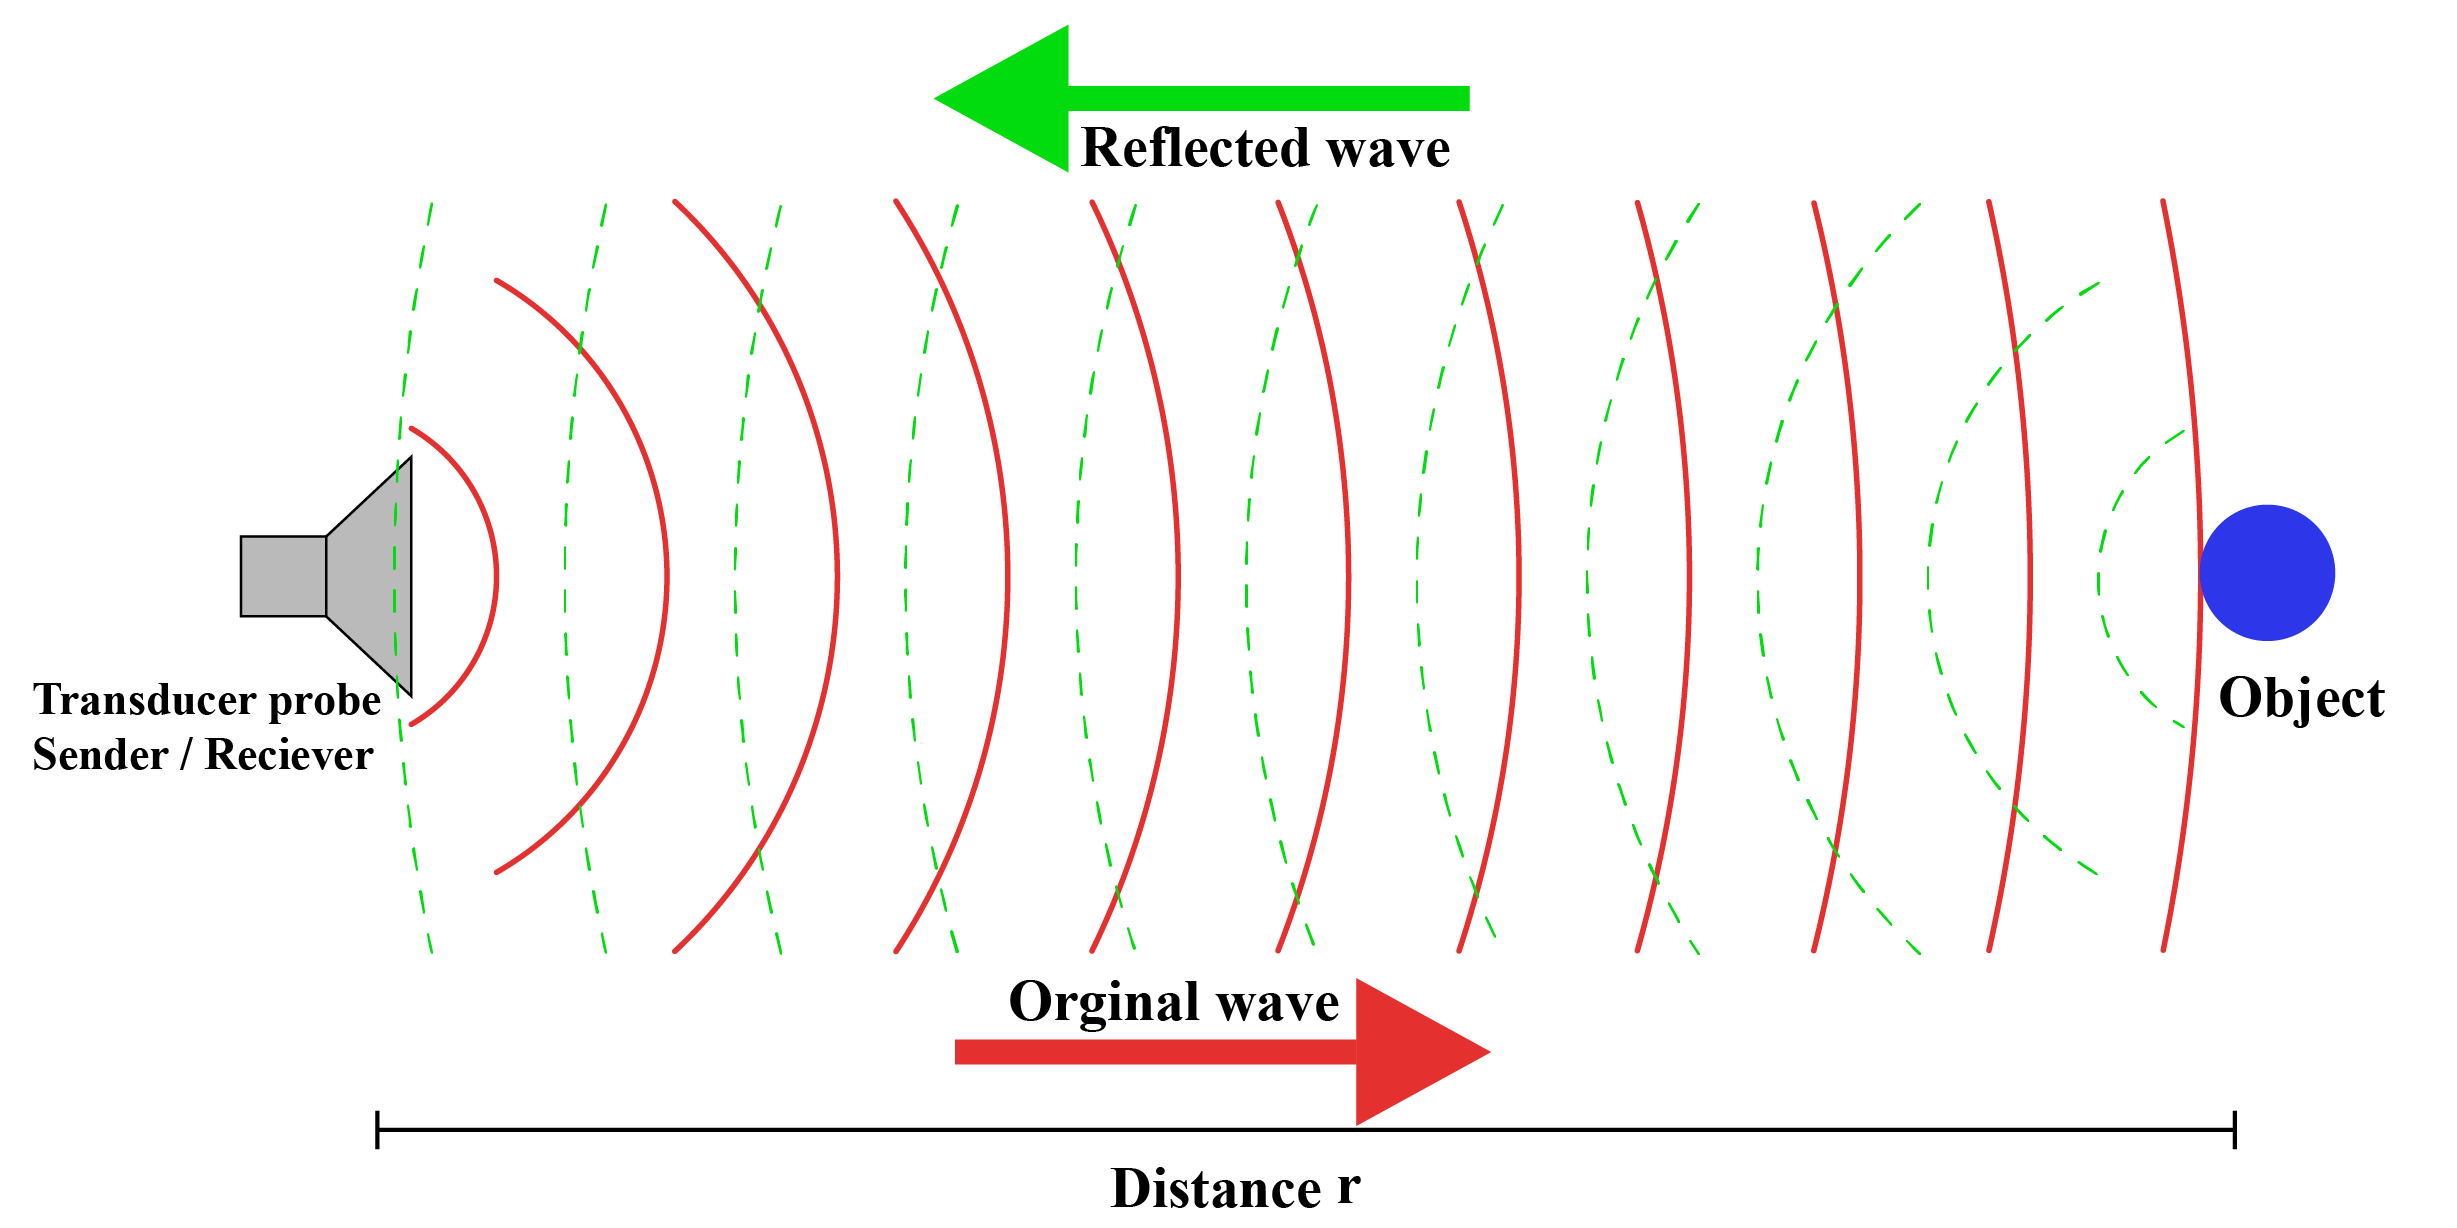
\includegraphics[width=0.7\columnwidth]{./figures/Fig11.png}
	\caption{how ultrasound works}
	\label{fig11}
\end{figure}

Interference between waves is the concept that helps to identify where the object is and what shape it is. In general, there is no control about where that object is located because, in 2d space, there is just 1d way of figuring out where the obstruction is located. The solution to this problem is to use more transducers. For example, consider we use two transducers, and they fire at the same time. The phase of the two waves is the same. Figure \ref{fig12} show this scenario. Although they come from two different sources, there is constructive interference between these two waves. So these are some points that have the highest magnitude.

\begin{figure}[htbp]
	%\resizebox{\linewidth}{!}{
	\centering 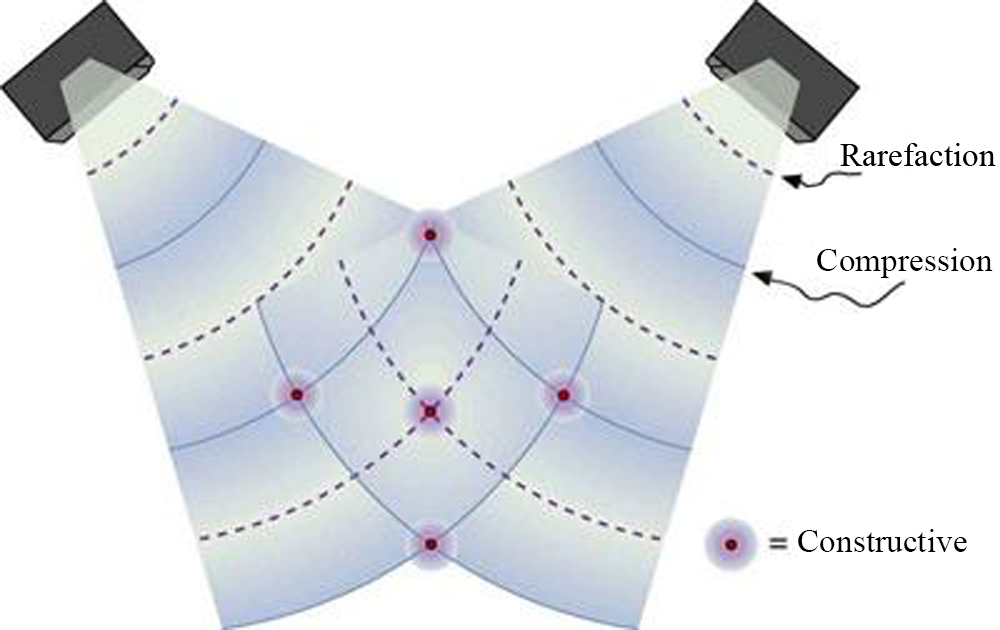
\includegraphics[width=0.7\columnwidth]{./figures/Fig12.jpg}
	\caption{how ultrasound works}
	\label{fig12}
\end{figure}

\section{Optical Microscopy and Molecular Imaging}

The last module which we cover is Optical Microscopy and Molecular imaging. The previous modules such as CT, MR, and Ultrasound are the majority of macro imaging modalities. In other words, in these modules, you look into larger parts of the body. In microscopy, you will look into a particular part of the body. This modality aims to study one single cell or a cluster of cells that was not possible with any other modalities.

A microscope usually does optical Microscopy and Molecular imaging. One of the first types of microscopy used in medical applications was the Single Photon Emission Computed Tomography (SPECT) system which was very useful to look into gamma photon generation. In this system, radio isotropy was put down along with glucose and give to the patient. If a particular organ has more glucose consumption, it means other organs are in there, and we would see more radionuclide coming down from there.

The resolution of SPECT was much lower and did not give a very high structural resolution. So, generally, structural scan systems are used either a structural CT or structural MR along with a SPECT. These multiple images are registered together to diagnose by knowing the structure and the function.

The other type of microscopy is Positron Emission Tomography, and when there is a positron emitted, you would see a pair of gamma photons created; this means that we always need to have a pair of detectors that are 180 degrees apart and if these detectors rotate we will be sensing a pair of incidences. This method helps to reduce noise, and the noises on each detector are independent. Figure \ref{fig13} shows this method. 

\begin{figure}[htbp]
	%\resizebox{\linewidth}{!}{
	\centering 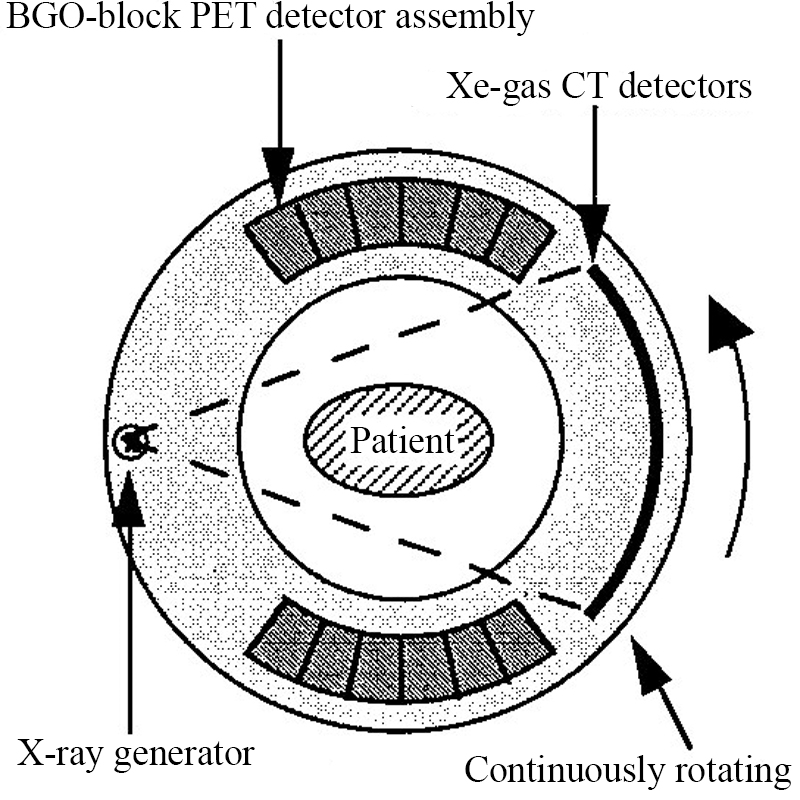
\includegraphics[width=0.7\columnwidth]{./figures/Fig13.jpg}
	\caption{Optical PET imaging instrument}
	\label{fig13}
\end{figure}


\chapter{Image processing concepts \& techniques}
\label{sec:chap4}

\section{Texture in medical images}
The texture is a variation of data at scales smaller than the scales of interest. For example, if we take an MR image from the human brain, any variation in the gray values of the imaged brain may be thought of as texture. Sometimes variation due to noise may be considered as texture. The texture is an intrinsic property of an image, and it is a valuable cue to recognize an object in the image.

The most important characteristic of texture is that it is scale-dependent. In other words, different types of textures are visible at different scales. For example, if we look at a section of the brain through a microscope, we will see a different structure of the tissue than sulci monitored. So, to use texture for identifying different types of tissue, we should be able to measure image texture in a repeatable and reliable way. In other words, it is necessary to characterize texture in an objective way, independent of human perception and visual abilities.

Structural or statistical methods may characterize texture. A structural method identifies a texture primitive pattern, and this pattern is repeated to create the viewed appearance. This approach is also known as grammars for texture description. Usually, structure methods are less common in biomedical applications. The other types of methods are statistical approaches, and they are more attractive. Figure \ref{fig14} shows how natural the transition from deterministic methods to statistical methods is. In this figure, we may easily infer from the first case in the left that a possible texture would be one surrounded by four 0s according to the other neighboring positions. But in the second case, we can see, in 7 out of 12 points, the arrangement of four 0s indicates a 1 in the middle, while in the remaining 5 cases, it indicates a 2. So the missing value has a probability of 58\% to be one and a chance of 42\% to be 2. This method is known as Markov Random Field (MRF) modeling.

\begin{figure}[htbp]
	%\resizebox{\linewidth}{!}{
	\centering 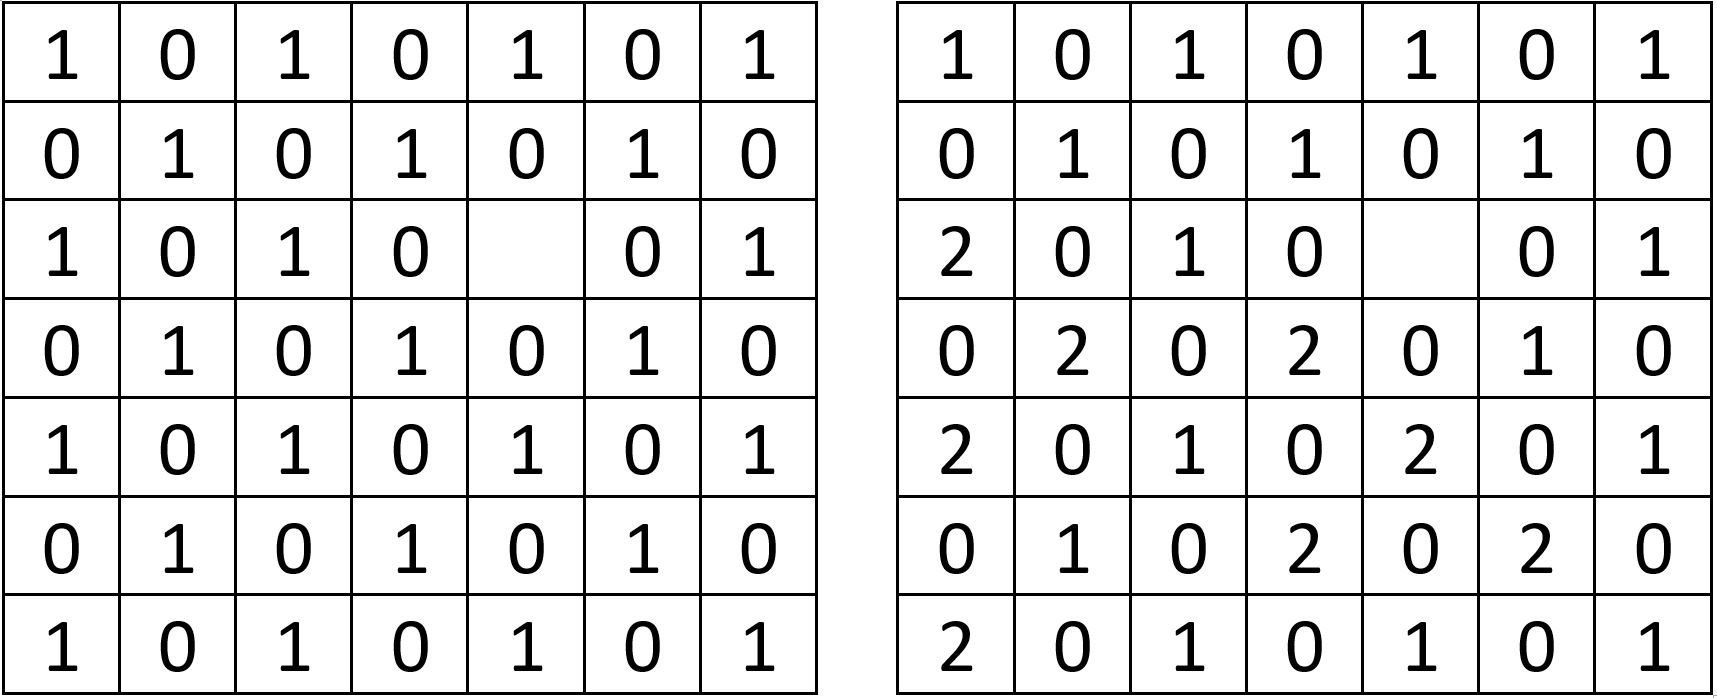
\includegraphics[width=0.6\columnwidth]{./figures/Fig14.jpg}
	\caption{Optical PET imaging instrument}
	\label{fig14}
\end{figure}

In MRF, we model the probability with which the neighbors' values are used to characterize the texture. As the statistics have to be performed on neighbor value combinations, and as pixels, particularly in medical images, take up many gray values, one needs an extensive sample of the texture to work out these parameters.

One of the issues in MRF texture approaches is the definition of the size of the neighborhood. In the previous example, we considered the smallest possible neighborhood. However, the neighborhood may be much larger to include pixels further away from the focal pixel. In the extreme case, all other pixels in the image are thought of as neighbors. In other words, the value of a pixel is directly influenced by all of the other pixels, and all scales of influence are essential.

In MRF texture descriptors, each pixel's value depends on the values of the neighbors, which have values that depend on their neighbors, and so on. The fractal models model this global dependence \textbf{explicitly}, while MRF models this global dependence \textbf{implicitly}. So, the MRF formulation leads to a formulation that models the \textbf{joint} probability density function of a particular combination of values of the whole image. Indeed, under certain conditions, an MRF modeling is equivalent to a Gibbs modeling.

Gibbs model is called clique potentials. A clique is a set of grid positions that are neighbors of each other according to the Markov model, therefore, directly influence each other’s value according to this model. In figure 10, the only cliques one can have are pairs of pixels next to each other, either vertically or horizontally. In Gibbs formalism, some parameters multiply the difference of the pairs of values of neighboring pixels to express their dependence. These parameters characterize the texture.

Gibbs distributions are not very useful in texture descriptions. However, they are beneficial in other problems of medical image processing, such as image restoration or image matching. What is important to us is how to move from local description (neighborhood-dependent modeling) to a global (joint probability).

Another noticeable transform before proceeding to quantify texture is to transform the image to the spatial frequency domain. The Discrete Fourier Transform (DFT) identifies the content of an image. DFT is complex but usually adopts its magnitude, which is known as the power spectrum. The power spectrum helps us to identify the periodicities are present in the texture.  

If we want to analyze the frequency content of the image in terms of different frequency ranges (bands), it is necessary to isolate bands in the frequency domain. Band isolation can be done with the help of some window centered at a particular frequency, and it will separate the required band. The most commonly used window is the \textbf{Gaussian} because it does not create artifacts in the image. Figure \ref{fig15} illustrates the process of band isolation.

\begin{figure}[htbp]
	%\resizebox{\linewidth}{!}{
	\centering 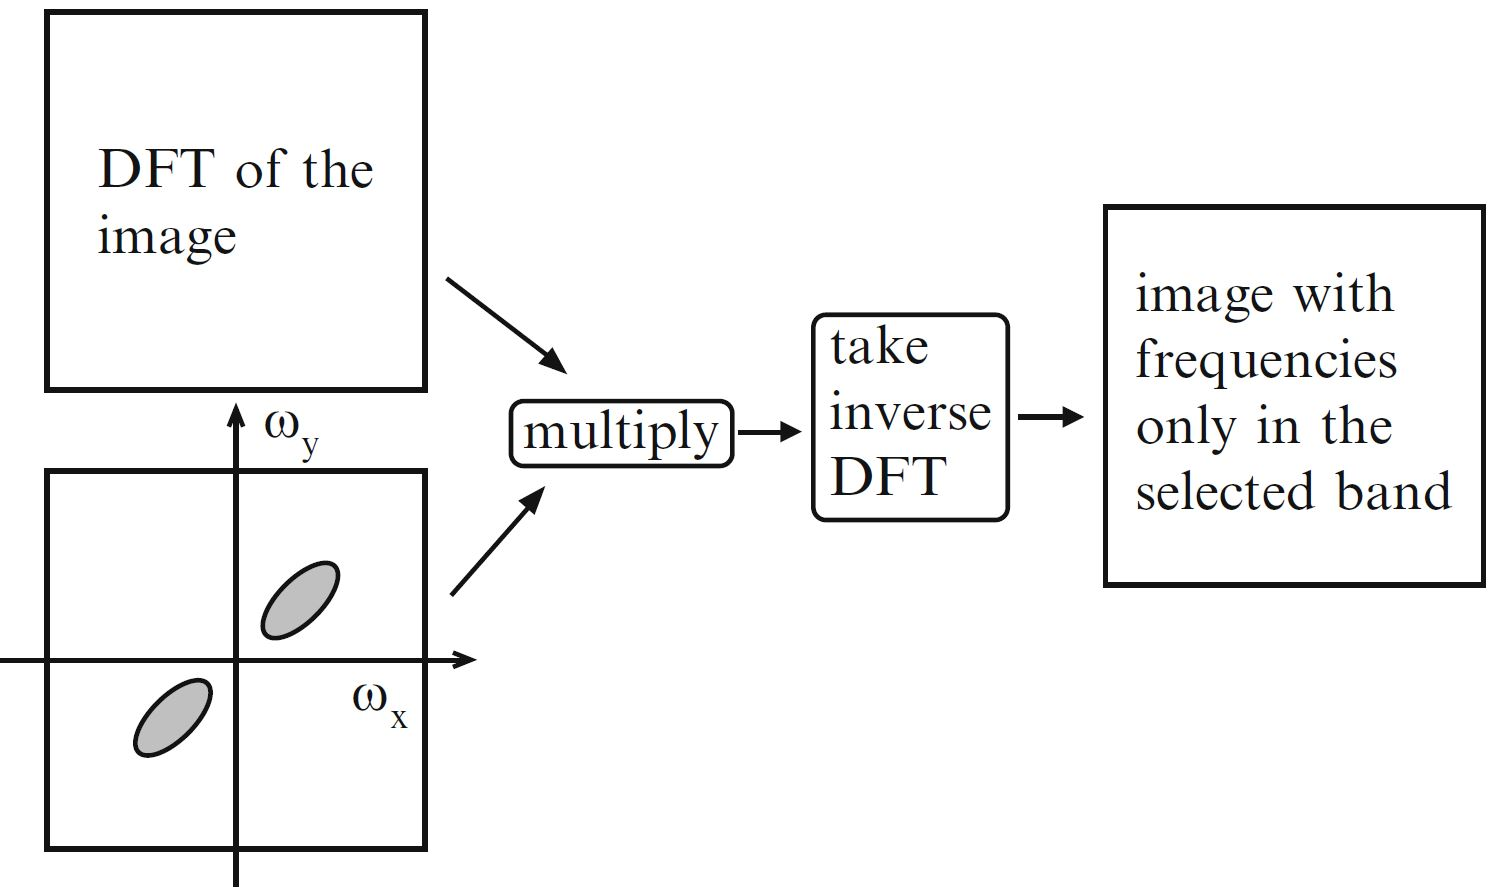
\includegraphics[width=0.6\columnwidth]{./figures/Fig15.jpg}
	\caption{Optical PET imaging instrument}
	\label{fig15}
\end{figure}

After extracting selected bands, we can compute features from them to characterize texture. The most helpful feature is the sum of the squares of the values of the output image. This feature is to find its energy in the particular frequency band.


\section{Segmentation}

The segmentation purpose is to split the image into parts, which are specific applications. The quality of the image segmentation scheme is estimated according to factors like Similarity Index, Dice Score, Sensitivity or Overlap fraction, Extra Fraction, Specificity, and Accuracy. For example, the Similarity Index (SI) tells about the mutual value among input MRI brain images and segmented output images. Accuracy is cast off to estimate the accomplishment of the tumor detection and segmentation system.

In medical imaging, segmentation often refers to the explanation of specific structures. So, it includes details of classification methods. Segmentation strategies in medical imaging combine data knowledge with domain knowledge to arrive at the result. Data knowledge refers to assumptions about continuity, homogeneity, and local smoothness of image features within segments. Domain knowledge represents information about the objects to be delineated.

Quantitative analysis of medical images requires objects or object features in the image to be identified. First, the image is segmented into regions that are the possible candidates of objects. This is followed by assigning meaning to these regions. For analyzing a digital photograph, \textbf{the segmentation} task would group pixels to areas that may belong to parts of objects based on the attributes of these regions. Hence, segmentation of images is similar to creating phonemes in speech or detecting syllables in written text. It means that the segmentation of images creates basic semantic entities from images.

However, it isn't easy to apply domain knowledge about objects in an image to segmentation. The purpose of segmentation is to create semantic entities in the first place. After segmentation, every pixel is assigned to exactly one segment since every location in an image carries just one meeting. The problem is appearances of objects in some images may be very different within and between objects classes. For example, Figure \ref{fig16} is a set of pictures contain a landscape with a house in the foreground, some trees and mountains in the background.

\begin{figure}[htbp]
	%\resizebox{\linewidth}{!}{
	\centering 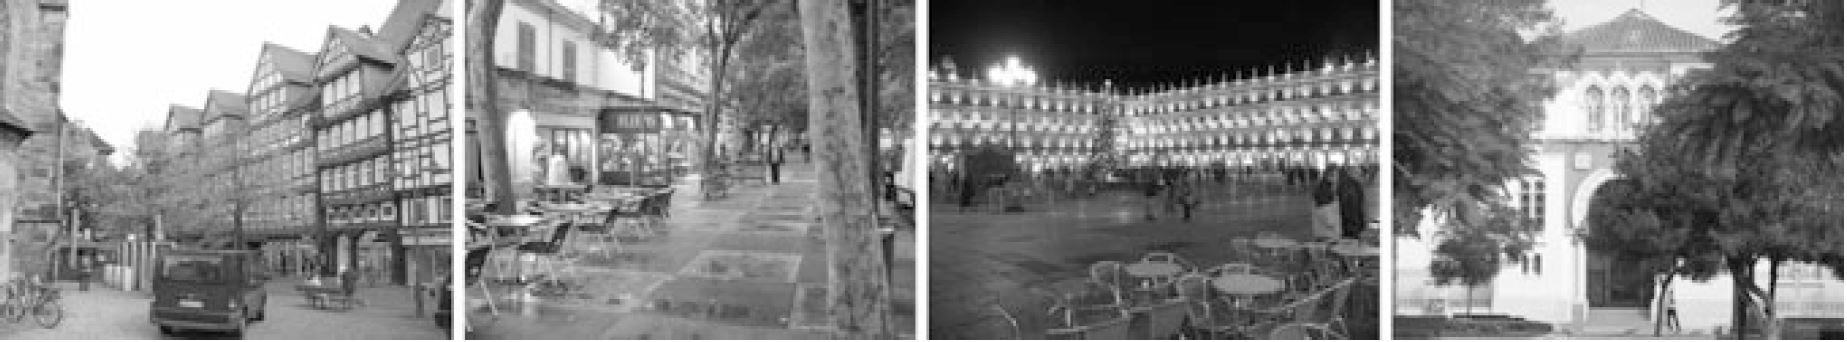
\includegraphics[width=0.7\columnwidth]{./figures/Fig16.jpg}
	\caption{Finding a general solution (find  houses) for a segmentation task}
	\label{fig16}
\end{figure}

For the segmentation of medical images, the situation is even worse, as a medical image represents the measurement of a diagnostically relevant entity measured in the same way everywhere in the body. For instance, consider a CT where X-ray attention is calculated on the normalized Hounsfield scale. Attention should not vary with location but only with density and atomic number.


There are several ways to deal with missing information without missing the assumption that a low-level segmentation criterion is valid everywhere in the image.

\textbf{Foreground segmentation} focuses on a single object in the image. Segmentation criteria create an excellent partitioning of foreground objects, whereas the quality of partitioning the background is irrelevant. The strategy requires some model knowledge to be applied after segmentation for separating foreground segments from the background. A simple way to introduce the model would be let the user point out foreground segments. Figure \ref{fig17} is an example of segmenting liver in a CT image.

\begin{figure}[htbp]
	%\resizebox{\linewidth}{!}{
	\centering 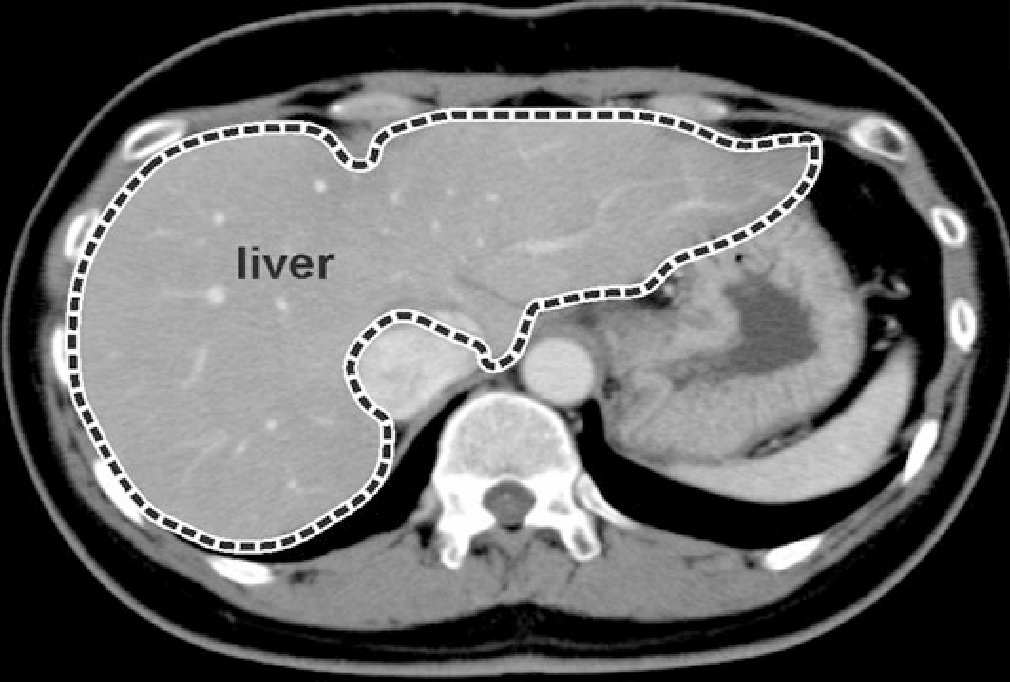
\includegraphics[width=0.6\columnwidth]{./figures/Fig17.jpg}
	\caption{Segmentation of liver from all other tissues}
	\label{fig17}
\end{figure}

\textbf{Hierarchical segmentation} (Figure \ref{fig18}) applies a multi-resolution concept for gradual refinement. A first segmentation creates segments that are smaller than the smallest object. It is assumed that a common criterion can be found at this scale. The result is sometimes called over-segment. Some of these segments are merged into larger segments at the next level according to domain knowledge about object appearance. Successful application of this strategy requires that common criteria define meaningful segments at a single but unknown scale. This scale is found by analyzing the levels of the segmentation hierarchy.


\begin{figure}[htbp]
	%\resizebox{\linewidth}{!}{
	\centering 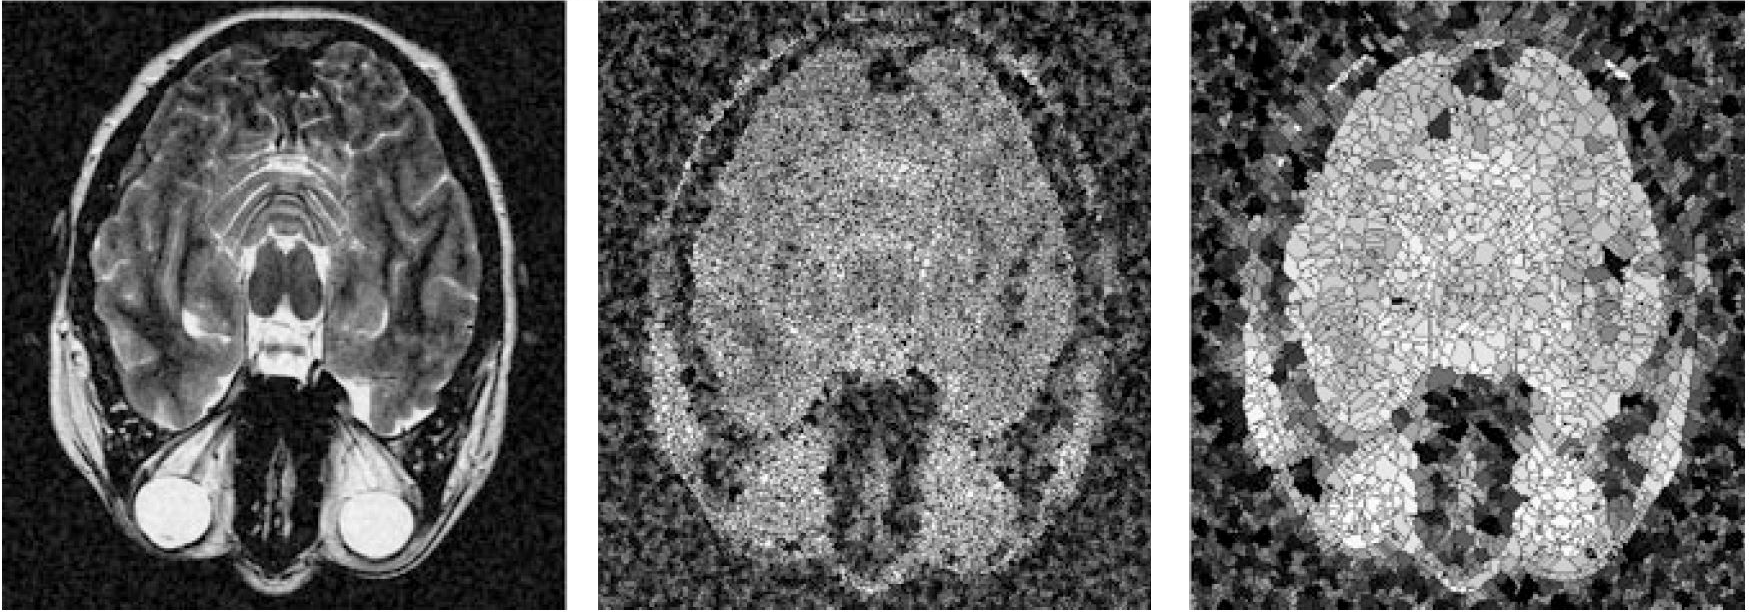
\includegraphics[width=0.55\columnwidth]{./figures/Fig18.png}
	\caption{hierarchical segmentation different stages}
	\label{fig18}
\end{figure}

\textbf{Multilayer segmentation} is another multi-resolution technique. It is assumed that a common segmentation criterion exists but that its scale may vary throughout the image (like the structured texture of an object in which the scale varies with the distance of the object to the camera). Segmentation is carried out at different scales producing layers of segments. Multilayer segmentation is more general than the previous strategy. The criterion scale often varies because an appropriate scale for every segment has to be established independently from other segments. Figure \ref{fig19} illustrates steps of multilayer segmentation. 

\begin{figure}[htbp]
	%\resizebox{\linewidth}{!}{
	\centering 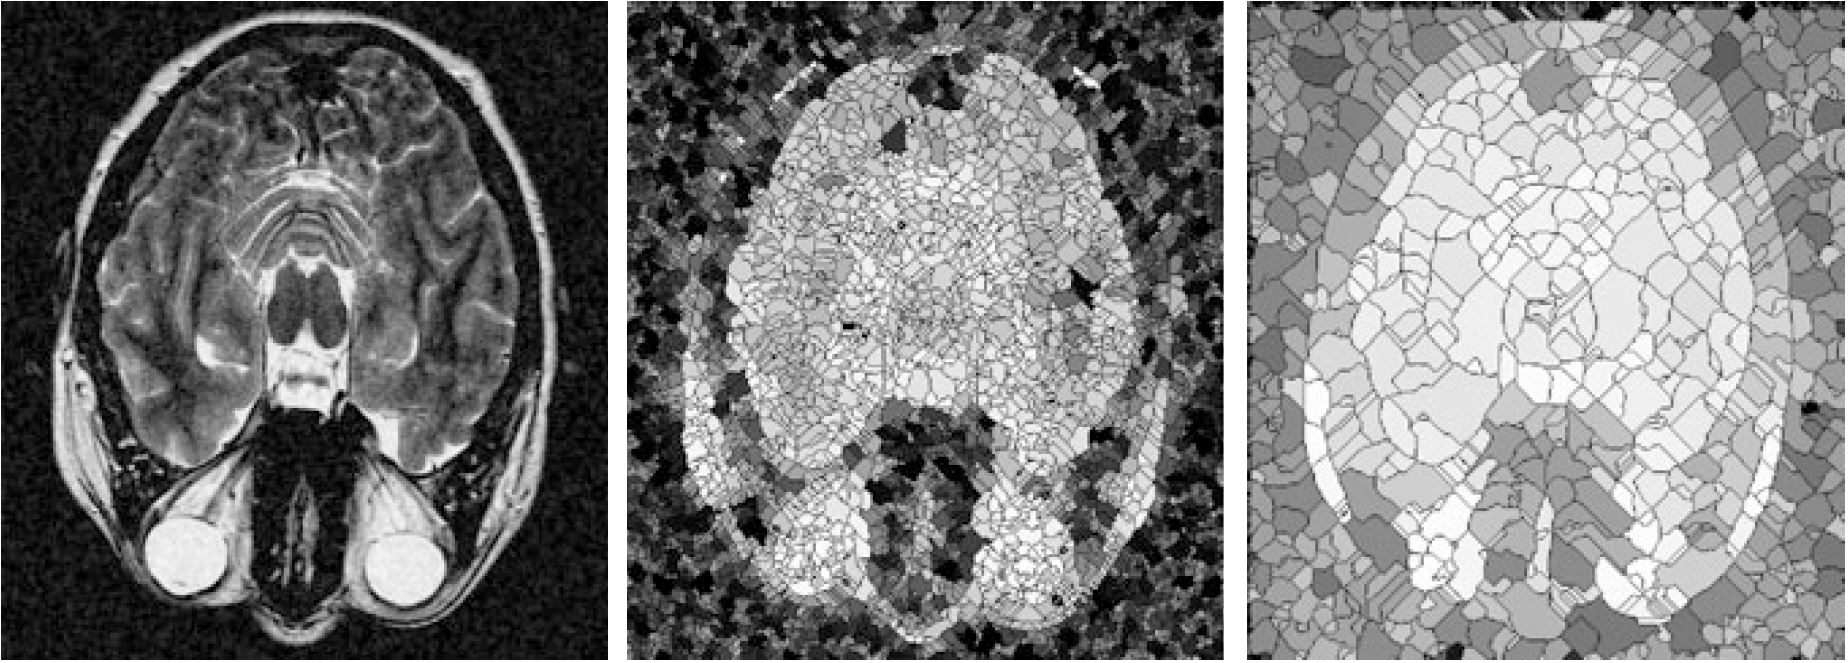
\includegraphics[width=0.55\columnwidth]{./figures/Fig19.png}
	\caption{segmentation at different levels of resolution are evaluated in parallel}
	\label{fig19}
\end{figure}

The search for a specific structure by segmentation causes foreground segmentation to be more frequent in medical image analysis than in other image analysis tasks. Since it may involve a detection task, a model-driven approach then discriminates the structure from the background. Model knowledge may be integrated into the algorithm or supplemented interactively. Popular segmentation techniques, such as the various region growing, active contours and surfaces, and active shape models, use a model-driven approach.

\section{Thresholding}

Thresholding is the simplest method of image segmentation. Various thresholding techniques are:
\begin{enumerate}
	\item \textbf{Global Thresholding}: In this method, we use a bimodal image. A bimodal image is an image with 2 peaks of intensities in the intensity distribution plot. One for the object and one for the background. Then we deduce the threshold value for the entire image and use that global threshold for the whole image. A disadvantage of this type of threshold is that it performs really poorly during poor illumination in the image(Figure \ref{fig21}).
	
	\begin{figure}[htbp]
		%\resizebox{\linewidth}{!}{
		\centering 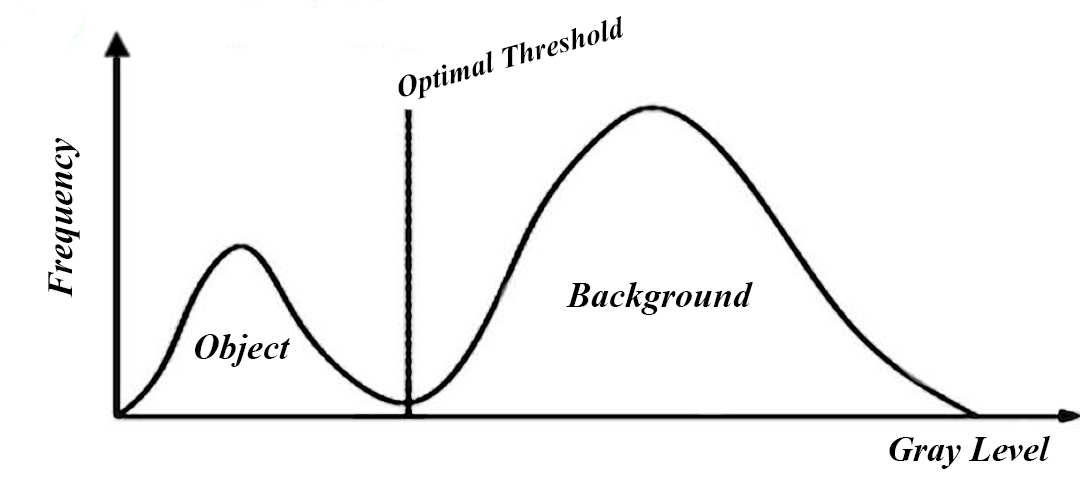
\includegraphics[width=0.55\columnwidth]{./figures/Fig21.jpg}
		\caption{Global Thresholding}
		\label{fig21}
	\end{figure}
	
	\item \textbf{Multimodal Thresholding}: A general approach to thresholding is based on assumption that images are multimodal, that is, different objects of interest relate to distinct peaks (or modes) of the 1D signal histogram. The thresholds have to optimally separate these peaks in spite of typical overlaps between the signal ranges corresponding to individual peaks(Figure \ref{fig22}).
	
	\begin{figure}[htbp]
		%\resizebox{\linewidth}{!}{
		\centering 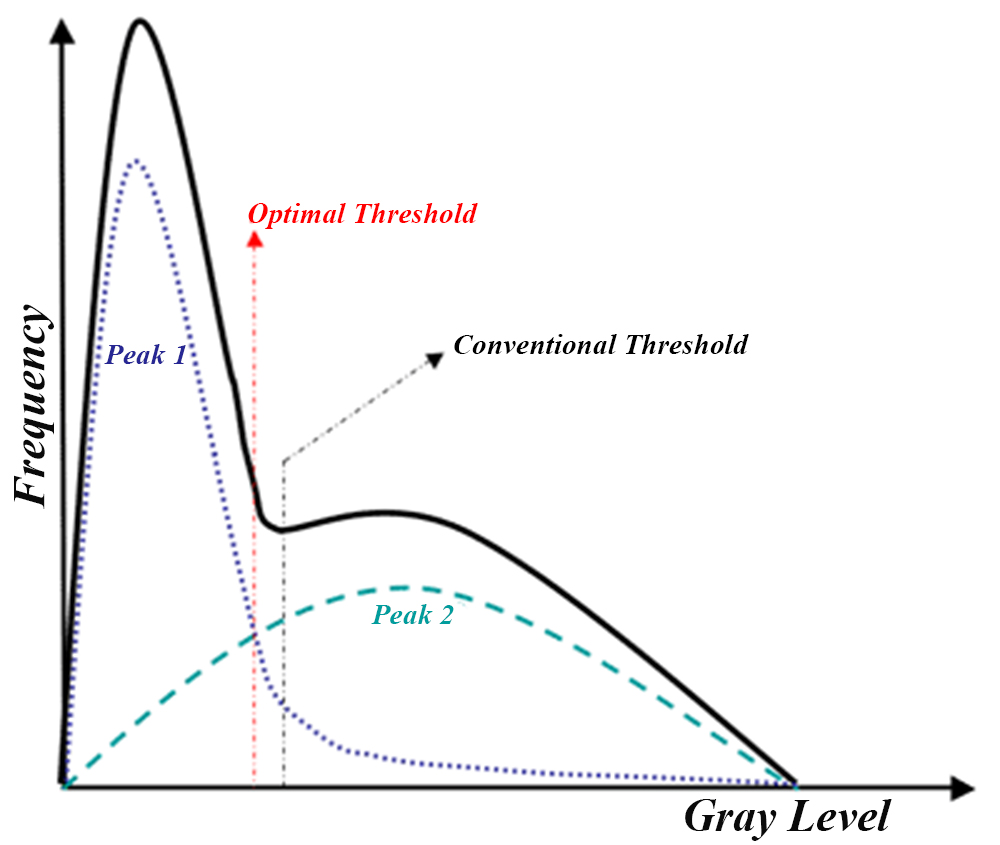
\includegraphics[width=0.55\columnwidth]{./figures/Fig22.jpg}
		\caption{Multimodal Thresholding}
		\label{fig22}
	\end{figure}
	
	\item \textbf{Adaptive Thresholding}: The image is divided into various subregions, and all these regions are segmented using the threshold value calculated for all these regions. Then these subregions are combined to image the complete segmented image. This helps in reducing the effect of illumination to a certain extent.
	
\end{enumerate}



\section{Artificial Neural Network}

ANN stands for Artificial Neural Network. Just like humans have BNN i.e. the Biological Neural Network, the researchers tried to replicate the working of the human brain and came up with the great invention of an Artificial Neural Network. ANNs have been developed for a wide range of applications such as function approximation, feature extraction, optimization, and classification. In particular, they have been developed for image enhancement, segmentation, registration, feature extraction, and object recognition.

There are three types of learning in ANN. They are supervised learning, unsupervised learning and reinforced learning. \textbf{Supervised learning} is based on error between output and input data. A teacher or supervisor is offered during learning process and offered projected output. In \textbf{Unsupervised learning} no teacher is presented to teach to the network. Unsupervised learning is very complex and difficult to implement. The system learns of its own by discovering and adapting to the structural features in the input sample of data. \textbf{Reinforced learning} is output based learning. Although a teacher existed during the procedure but, the teacher is not going to present the actual output. The teacher only indicated whether the output is correct or incorrect.

\section{Clustering}
Clustering is a type of unsupervised machine learning algorithm. It is highly used for the segmentation of images. One of the most dominant clustering-based algorithms used for segmentation is KMeans Clustering. This type of clustering can be used to make segments in a colored image. Three main clustering methods are as follows:

\begin{enumerate}
	\item \textbf{Traditional Clustering}
	\item \textbf{Hierarchical Clustering}: Also called Hierarchical cluster analysis or \textbf{HCA} is an unsupervised clustering algorithm. The algorithm groups similar objects into groups called clusters. The endpoint is a set of clusters that have ordering from top to bottom.
	\item \textbf{Partitional Clustering}: These algorithms minimize a given clustering criterion by iteratively relocating data points between clusters until a (locally) optimal partition is attained. Famous \textbf{K-means clustering} comes under partitioning method.
\end{enumerate} 


\section{Edge Detection}

Edge-based segmentation relies on edges found in an image using various edge detection operators. These edges mark image locations of discontinuity in gray levels, color, texture, etc. When we move from one region to another, the gray level may change. So if we can find that discontinuity, we can find that edge. This process detects outlines of an object and boundaries between objects and the background in the
image. An edge-detection filter can also be used to improve the appearance of blurred image. A variety of edge detection operators are available but the resulting image is an intermediate segmentation result and should not be confused with the final segmented image. We have to perform further processing on the image to the segment it. Additional steps include combining edges segments obtained into one segment in order to reduce the number of segments.

Edges are usually associated with “Magnitude” and “Direction”. Some edge detectors give both directions and magnitude. We can use various edge detectors like Sobel edge operator, canny edge detector, Kirsch edge operator, Prewitt edge operator, Robert’s edge operator, etc.

\section{Region-Based}
A region can be classified as a group of connected pixels exhibiting similar properties. The similarity between pixels can be in terms of intensity, color, etc. In this type of segmentation, some predefined rules are present which have to be obeyed by a pixel in order to be classified into similar pixel regions. Region-based segmentation methods are preferred over edge-based segmentation methods in case of a noisy image. Region-Based techniques are further classified into 3 types based on the approaches they follow.

\begin{enumerate}
	\item \textbf{Region Growing}: We start with some pixel as the seed pixel and then check the adjacent pixels. If the adjacent pixels abide by the predefined rules, then that pixel is added to the region of the seed pixel and the following process continues till there is no similarity left.
	\item \textbf{Region Splitting}: The whole image is first taken as a single region. If the region does not follow the predefined rules, then it is further divided into multiple regions (usually 4 quadrants) and then the predefined rules are carried out on those regions in order to decide whether to further subdivide or to classify that as a region. This process continues till there is no further division of regions required
	\item \textbf{Splitting \& Merging}: In these methods, after splitting regions we consider every pixel as an individual region. We select a region as the seed region to check if adjacent regions are similar based on predefined rules. If they are similar, we merge them into a single region and move ahead in order to build the segmented regions of the whole image.
\end{enumerate}


\section{Graph-Based}

graph-based methods present different graph representations, where the nodes may be pixels, pixel vertices, regions, or user-drawn markers. They also differ in the graph algorithm used to solve the problem: graph matching, random walker, the min-cut/max-flow algorithm, Dijkstra's algorithm, Kruskal's or Prim's algorithm, etc. Figure \ref{fig23} illustrates how graph-based segmentation algorithms work.

\begin{figure}[htbp]
	%\resizebox{\linewidth}{!}{
	\centering 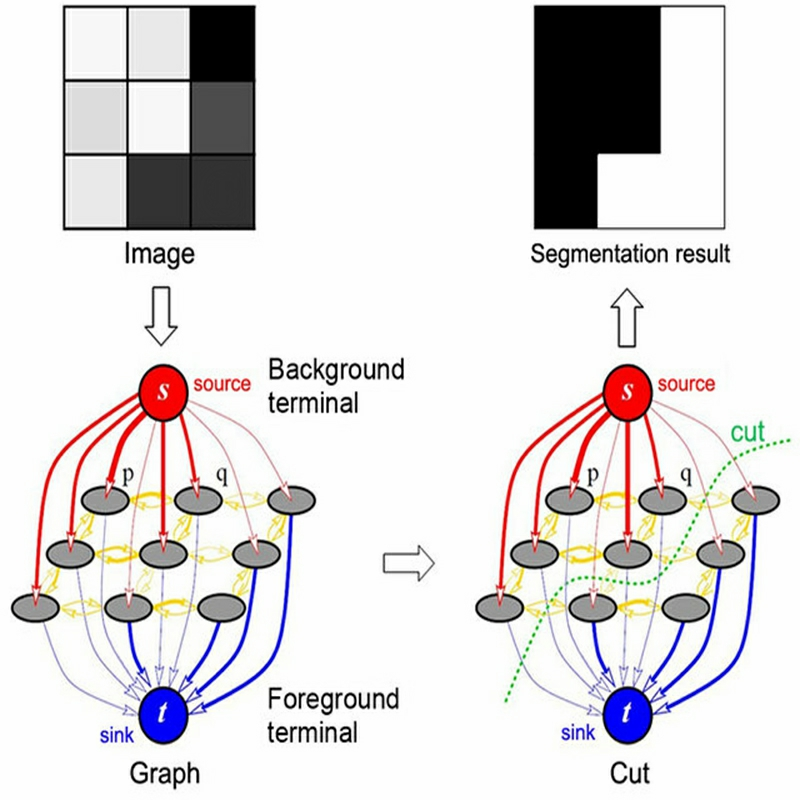
\includegraphics[width=0.65\columnwidth]{./figures/Fig23.jpg}
	\caption{Graph-based segmentation}
	\label{fig23}
\end{figure}


\section{Derformable Models}

Deformable models have been extensively studied and widely used in medical image segmentation, with promising results. Deformable
models are curves or surfaces defined within an image domain that can
move under the influence of internal forces, which are defined within the curve or surface itself, and external forces, which are computed from the image data. The internal forces are designed to keep the model smooth during deformation. The external forces are defined to move the model toward an object boundary or other desired features within an image.

\section{Watershed}
It is often used when we are dealing with one of the most difficult operations in image processing – separating similar objects in the image that are touching each other. To understand the “philosophy” behind the watershed algorithm we need to think of a grayscale image as a topographic surface. In such an image high-intensity pixel values represent peaks (white areas), whereas low-intensity values represent valleys – local minima (black areas). we start filling every isolated valley with water. the rising water from different valleys will start to merge. To avoid that, we need to build barriers in the locations where the water would merge. These barriers we call watershed lines and they are used to determine segment boundaries.


We described some of the most common strategies for segmenting medical images. Figure \ref{fig20} shows various approaches for segmentation.

\begin{figure}[htbp]
	%\resizebox{\linewidth}{!}{
	\centering 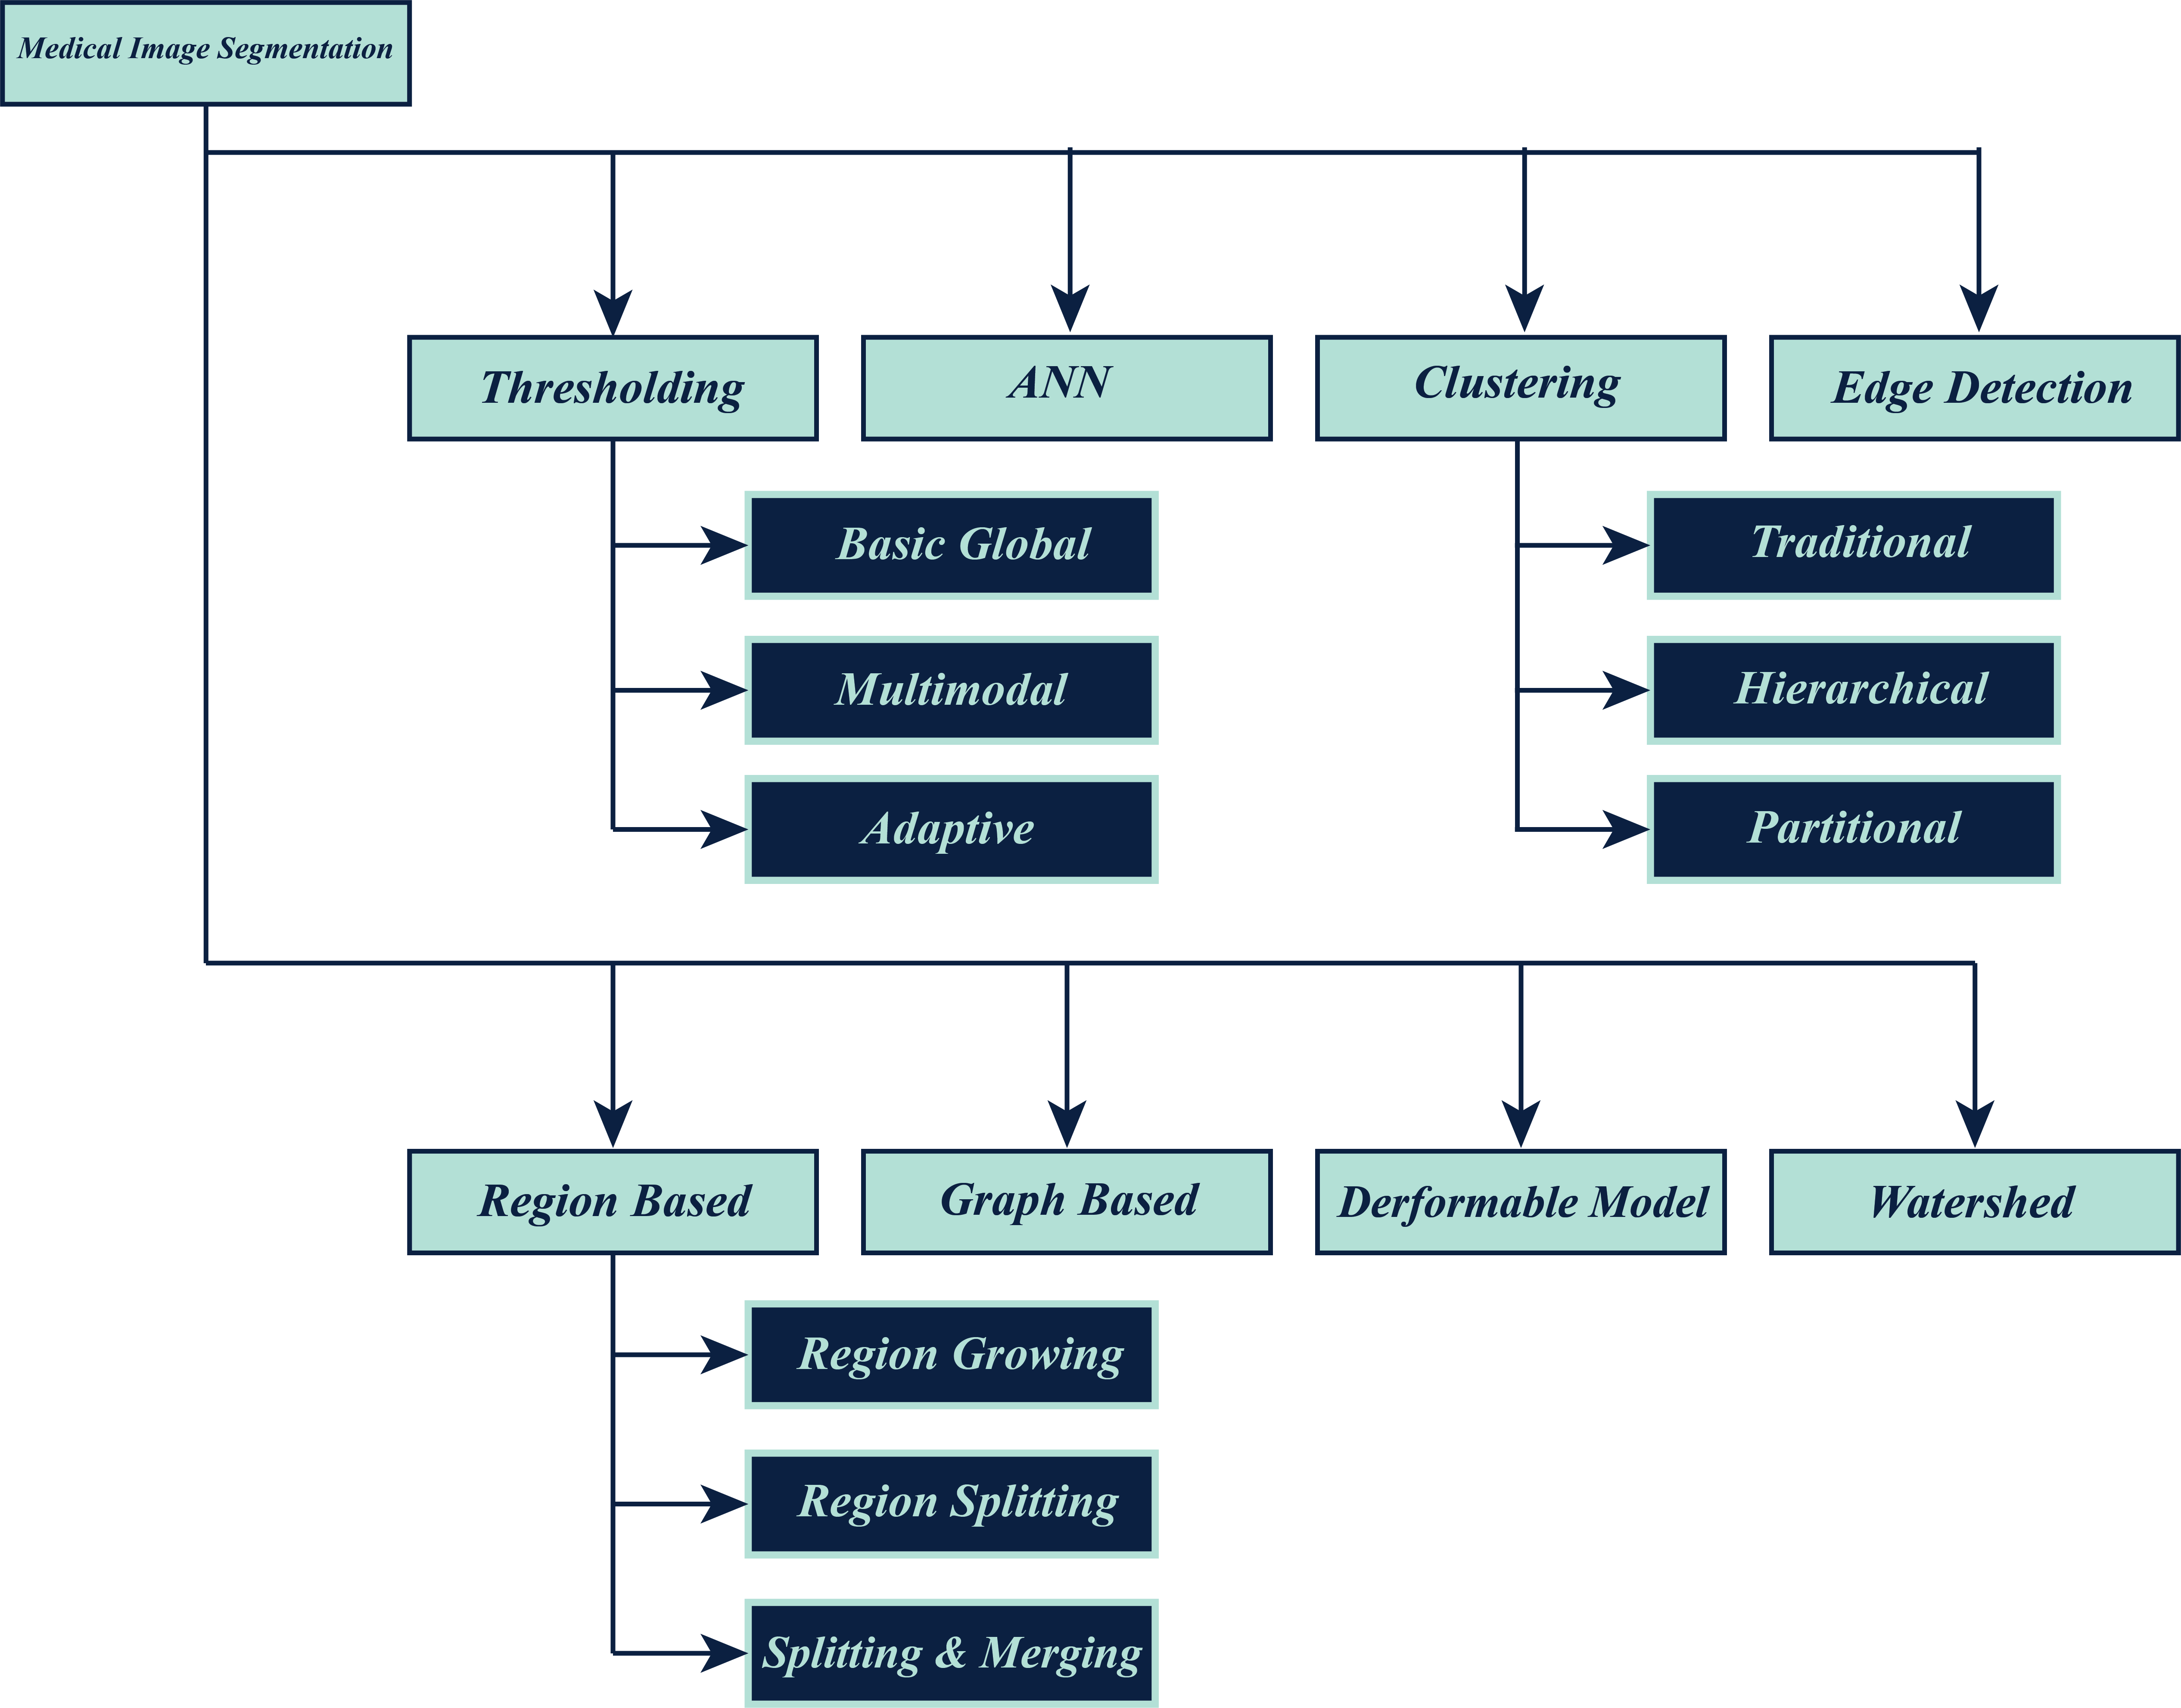
\includegraphics[width=0.75\columnwidth]{./figures/Fig20.png}
	\caption{segmentation techniques}
	\label{fig20}
\end{figure}

\section{Denoising}
Image denoising is required to use in digital image processing. From the researchers’ point of view, image denoising is still challenging task in medical images. Image denoising stays a normal process in digital image processing. It remains a pre-processing period to eradicate specific unidentified such as Additive White Gaussian Noise (AWGN) from an image to get a clean image used in favor of image processing, such as image segmentation. A representative instance of the image processor is image denoising prototypical. This method incorporates a disintegrated prototypical giving to some prior information of a corrupted image. To reestablish the distorted image in favor of obtaining a promising result. 

In this instance, \textit{$n_0$} tells about noisy medical image and $\textit{w}$ is an original, nevertheless usually known or unknown image i.e.,

\begin{equation}
	\centering
	n_0 = Dw + n_1
\end{equation}.

In which \textit{D} is a linear or non-linear operator representing the distortion and \textit{$n_1$} is additive noise.

The performance of the image denoising method is measured by using the essential factors such as Mean or Average pixel intensity, Standard Deviation, Mean Square Error, Root Mean Square Error, Mean Absolute Error, Peak Signal to Noise Ratio, Structural Similarity, Universal Image Quality Index, and Entropy. For example, the mean parameter determines the dissimilarity of the image by adding all the pixels and dividing the total pixels of the image. The average gradient gives the sharpness and clarity of the image.

There are other algorithms and general technologies designed intended for image denoising. These are listed below:

\section{Statistical modeling-based image denoising}

In 2018, Wang presented the minimax-concave TV (MCTV) to reconstruct the MR brain image. MCTV is non-convex, mainly to represent the nonconvexity parameter correctly and at the same time maintain a convexity for every iteration step.

In 2016, Park suggested a method of learning-based denoising. This method significantly reduces PI noise, and the start-up time is much faster. It creates high-quality images that do not have degrading information to increase speed. In the same year, Zhang demonstrated an MRI denoising framework that structurally correlates between users to evaluate the models efficiently to reduce noise in the signal.

\section{Derivative-based image denoising}
In 2017, Magudeeswaran developed a novel level-set technique originates from the active contour prototypical. This technique diminishes the costly initialization of a level set approach further efficiently. Primarily, images are pre-processed with the Contrast Limited Fuzzy Adaptive Histogram Equalization (CLFAHE) improvement technique to enhance the dissimilarity of the image.

In 2016, Sedaaghi solved PM flux analysis problems. In this method, the image remains bisected into three slices, depending on gradient level: the area where the slope is inferior to the smoothness of the area, where the slope is between the smoothness and the flux point, and the slope area is higher than the flux point. Also, in this year, Yang proposed an image denoising algorithm using PDE and GCV. In this method, the blocking effect is reduced by tetrolet transformation and is considered to be good.

To eradicate the staircase consequence aimed at TV filter and evading boundaries distorting in support of fourth-order PDE filter, Tan suggested the anisotropic diffusion in favor of image denoising. In this method, if the pixels are part of the flat area, a fourth-order filter is accepted that can remove the staircase artifacts. Figure \ref{fig24} illustrates these denoising methods in an abstract view.

\begin{figure}[htbp]
	%\resizebox{\linewidth}{!}{
	\centering \includegraphics[width=1\columnwidth,height=12cm]{./figures/Fig24.png}
	\caption{Image Denoising Methods}
	\label{fig24}
\end{figure}

%chapter 5 added to chapter 4
%\chapter{}
\label{sec:chap5}

\chapter{Hands on Python \& OpenCV}
\label{sec:chap6}
Magnetic Resonance Imaging (MRI) helps the healthcare field detect very minor abnormal growth in any part of the human being. While deep neural networks (NNs) and machine learning techniques have good achievement in 2D image segmentation, but it’s a challenging task for NNs to segment critical organs from 3D medical MR images. Segmentation relating to tumor detection includes several processing techniques categorized into Pre-Processing, Segmentation, Optimization, and Feature Extraction.

\section{Introduction to OpenCV}

\subsection{Installing OpenCV for Python}

\subsubsection{Windows}

In order to get OpenCV-Python up and running, we need to perform the following steps:

\begin{enumerate}
	\item \textbf{Install Python}:Make sure you have Python 3.8.x installed on your machine. If you don't have it, you can install it from \url{https://www.python.org/downloads/windows/}
	
	\item \textbf{Install NumPy}: NumPy is a great package to do numerical computing in Python. It is very powerful and has a wide variety of functions. OpenCV-Python plays nicely with NumPy, and we will be using this package a lot, during the course of this book. You can install the latest version from \url{http://sourceforge.net/projects/numpy/files/NumPy/}. We need to install all these packages in their default locations. Once we install Python and NumPy, we need to ensure that they're working fine. Open up the Python shell and type the following:
	
	\vspace{0.5cm}
	\colorbox{lgray}{\\\textbf{$>>>$ import numpy as np}}
	\vspace{0.5cm}
	
	If the installation has gone well, this shouldn't throw any error
	
	\item \textbf{Install Matplotlib}: Matplotlib is a comprehensive library for creating static, animated, and interactive visualizations in Python. We use pip package to install this library. Type the folloing script in your command prompt. 
	
	\vspace{0.5cm}
	\colorbox{lgray}{\\\textbf{pip install matplotlib}}
	\vspace{0.5cm}
	
	\item \textbf{Install OpenCV}:download the latest OpenCV version from \url{http://opencv.org/downloads.html}. Once you finish downloading it, double-click to install it. You're all set! Let's make sure that OpenCV is working. Open up the Python shell and type the following:
	
	\vspace{0.5cm}
	\colorbox{lgray}{\\\textbf{$>>>$ import cv2}}
	\vspace{0.5cm}
\end{enumerate}

\subsubsection{Linux (for Ubuntu)}
Let’s go ahead and build OpenCV with Python support. The commands below will install all packages necessary to run OpenCV.

\vspace{0.5cm}
\colorbox{lgray}{\\\textbf{\$ sudo apt update}}

\colorbox{lgray}{\\\textbf{\$ sudo apt install python3-opencv}}
\vspace{0.5cm}

To verify the installation, import the cv2 module and print the OpenCV version:

\vspace{0.5cm}
\colorbox{lgray}{\\\textbf{$>>>$ import cv2}}

\colorbox{lgray}{\\\textbf{$>>>$ print (cv2.\_\_version\_\_)}}
\vspace{0.5cm}

\subsection{Reading, Displaying, and Saving images}
Let's see how we can load an image in OpenCV-Python. Create a new jupyter notebook named \textbf{program 1}.  Create a folder named \textbf{images} in the current folder, and make sure that you have at least one	image with .jpg format in that folder. Once you do that, add the following lines of code to one of the Python cells. If you run the preceding program, you will see an image being displayed in a new window.

\vspace{0.2cm}

\begin{tcolorbox}[breakable, size=fbox, boxrule=1pt, pad at break*=1mm,colback=cellbackground, colframe=cellborder]
	\prompt{In}{incolor}{ }{\boxspacing}
	\begin{Verbatim}[commandchars=\\\{\}]
\PY{k+kn}{import} \PY{n+nn}{cv2}
	\end{Verbatim}
\end{tcolorbox}

\begin{tcolorbox}[breakable, size=fbox, boxrule=1pt, pad at break*=1mm,colback=cellbackground, colframe=cellborder]
	\prompt{In}{incolor}{ }{\boxspacing}
	\begin{Verbatim}[commandchars=\\\{\}]
\PY{n}{img} \PY{o}{=} \PY{n}{cv2}\PY{o}{.}\PY{n}{imread}\PY{p}{(}\PY{l+s+s1}{\PYZsq{}}\PY{l+s+s1}{images/Sample1.jpg}\PY{l+s+s1}{\PYZsq{}}\PY{p}{)}
\PY{n}{cv2}\PY{o}{.}\PY{n}{imshow}\PY{p}{(}\PY{l+s+s1}{\PYZsq{}}\PY{l+s+s1}{Sample 1}\PY{l+s+s1}{\PYZsq{}}\PY{p}{,}\PY{n}{img}\PY{p}{)}
\PY{n}{cv2}\PY{o}{.}\PY{n}{waitKey}\PY{p}{(}\PY{p}{)}
	\end{Verbatim}
\end{tcolorbox}

\begin{figure}[htbp]
	\centering 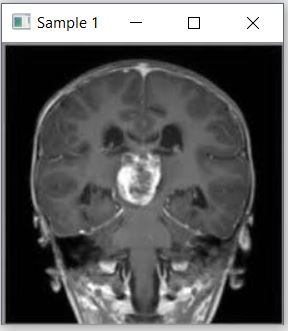
\includegraphics[width=0.45\columnwidth]{./figures/p1.jpg}
\end{figure}

Let's understand the previous piece of code, line by line. In the first line, we are importing the OpenCV 	library. We need this for all the functions we will be using in the code. In the second line, we are reading the image 	and storing it in a variable. OpenCV uses NumPy data structures to store the images. In the next line, we display the 	image in a new window. The first argument in \textbf{cv2.imshow} is the name of the window. The second argument is the 	image you want to display.

The function, \textbf{cv2.waitKey()}, is used in OpenCV for keyboard binding. It takes a number as an argument, and 	that number indicates the time in milliseconds. Basically, we use this function to wait for a specified duration, until we 	encounter a keyboard event. The program stops at this point, and waits for you to press any key to continue. If we 	don't pass any argument or if we pass 0 as the argument, this function will wait for a keyboard event indefinitely.

\subsection{Loading and Saving images}
OpenCV provides multiple ways of loading an image. Let's say we want to load a color image in grayscale mode. We can do that using the following piece of code:

\vspace{0.5cm}

\begin{tcolorbox}[breakable, size=fbox, boxrule=1pt, pad at break*=1mm,colback=cellbackground, colframe=cellborder]
	\prompt{In}{incolor}{ }{\boxspacing}
	\begin{Verbatim}[commandchars=\\\{\}]
\PY{k+kn}{import} \PY{n+nn}{cv2}
	\end{Verbatim}
\end{tcolorbox}

\begin{tcolorbox}[breakable, size=fbox, boxrule=1pt, pad at break*=1mm,colback=cellbackground, colframe=cellborder]
	\prompt{In}{incolor}{ }{\boxspacing}
	\begin{Verbatim}[commandchars=\\\{\}]
\PY{n}{normal\PYZus{}img} \PY{o}{=} \PY{n}{cv2}\PY{o}{.}\PY{n}{imread}\PY{p}{(}\PY{l+s+s1}{\PYZsq{}}\PY{l+s+s1}{images/Sample2.jpg}\PY{l+s+s1}{\PYZsq{}}\PY{p}{)}
\PY{n}{gray\PYZus{}img} \PY{o}{=} \PY{n}{cv2}\PY{o}{.}\PY{n}{imread}\PY{p}{(}\PY{l+s+s1}{\PYZsq{}}\PY{l+s+s1}{images/Sample2.jpg}\PY{l+s+s1}{\PYZsq{}}\PY{p}{,}\PY{n}{cv2}\PY{o}{.}\PY{n}{IMREAD\PYZus{}GRAYSCALE}\PY{p}{)}
\PY{n}{cv2}\PY{o}{.}\PY{n}{imshow}\PY{p}{(}\PY{l+s+s1}{\PYZsq{}}\PY{l+s+s1}{Normal image}\PY{l+s+s1}{\PYZsq{}}\PY{p}{,}\PY{n}{normal\PYZus{}img}\PY{p}{)}
\PY{n}{cv2}\PY{o}{.}\PY{n}{imshow}\PY{p}{(}\PY{l+s+s1}{\PYZsq{}}\PY{l+s+s1}{Gray Scale image}\PY{l+s+s1}{\PYZsq{}}\PY{p}{,}\PY{n}{gray\PYZus{}img}\PY{p}{)}
\PY{n}{cv2}\PY{o}{.}\PY{n}{waitKey}\PY{p}{(}\PY{p}{)}
	\end{Verbatim}
\end{tcolorbox}

\begin{figure}[htbp]
	\centerline{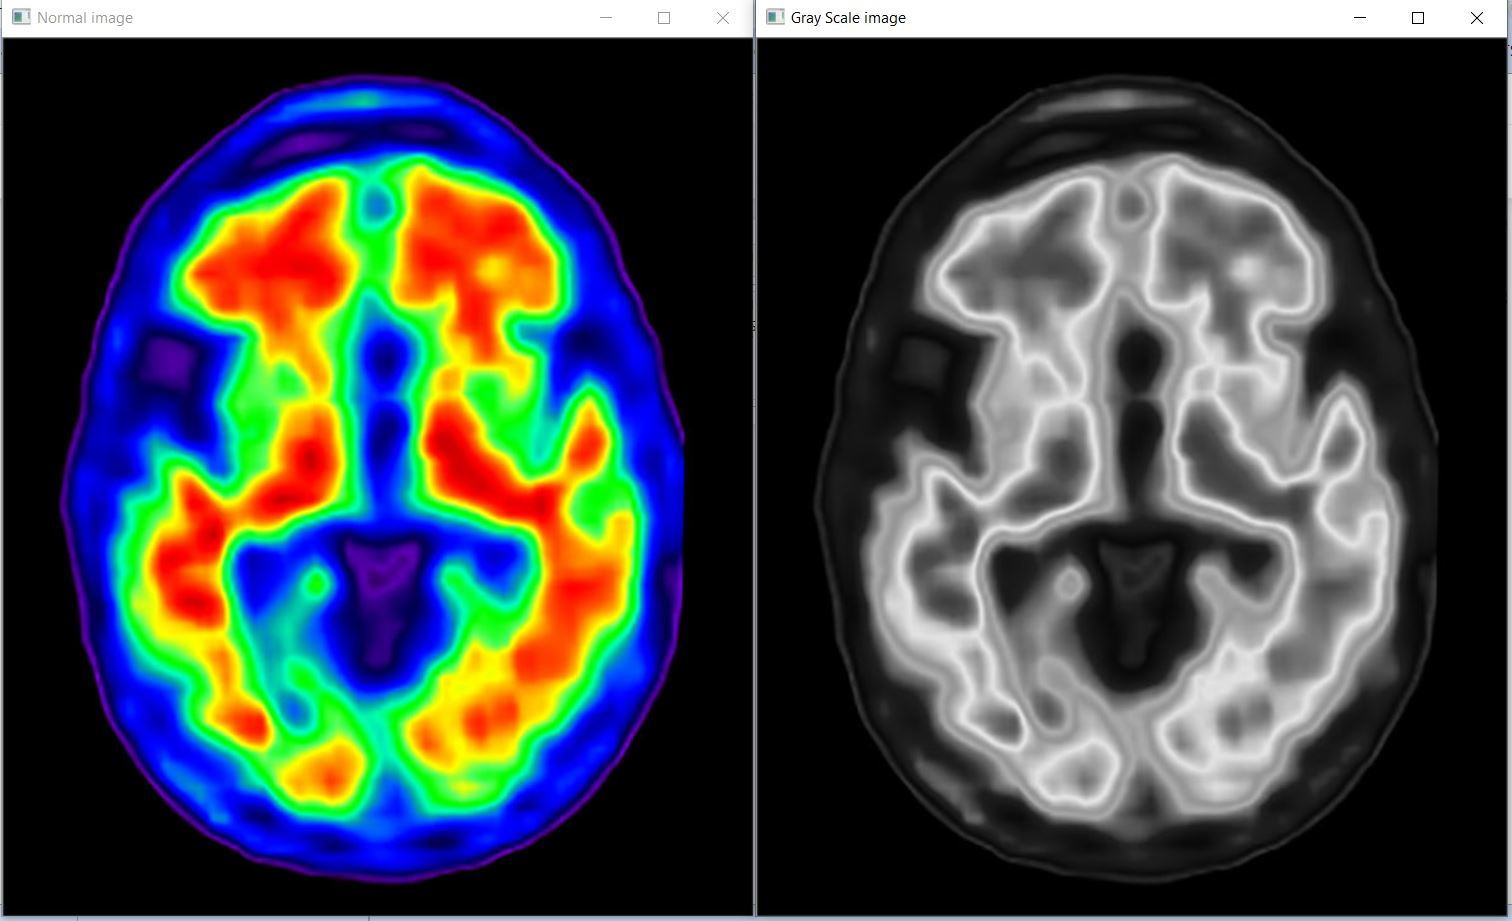
\includegraphics[width=0.8\columnwidth]{figures/p2.jpg}}
\end{figure}

Here, we are using the flag \textbf{cv2.IMREAD\_GRAYSCALE} to load the image in grayscale mode. You can see that from the 	image being displayed in the new window. We can save this image into a file as well:

\vspace{0.5cm}

\begin{tcolorbox}[breakable, size=fbox, boxrule=1pt, pad at break*=1mm,colback=cellbackground, colframe=cellborder]
	\prompt{In}{incolor}{ }{\boxspacing}
	\begin{Verbatim}[commandchars=\\\{\}]
\PY{n}{cv2}\PY{o}{.}\PY{n}{imwrite}\PY{p}{(}\PY{l+s+s1}{\PYZsq{}}\PY{l+s+s1}{images/output.jpg}\PY{l+s+s1}{\PYZsq{}}\PY{p}{,}\PY{n}{gray\PYZus{}img}\PY{p}{)}
	\end{Verbatim}
\end{tcolorbox}

This will save the grayscale image into an output file named \textbf{output.jpg}.

\subsection{Image color spaces}
In computer vision and image processing, color space refers to a specific way of organizing colors. A color space is actually a combination of two things: a color model and a mapping function. The reason we want color models is because it helps us in representing pixel values using tuples. The mapping function maps the color model to the set of all possible colors that can be represented.

There are many different color spaces that are useful. Some of the more popular color spaces are RGB, YUV, 	HSV, Lab, and so on. Different color spaces provide different advantages. We just need to pick the color space that's 	right for the given problem. Let's take a couple of color spaces and see what information they provide:

\begin{itemize}
	\item \textbf{RGB}: It's probably the most popular color space. It stands for Red, Green, and Blue. In this color space, each 	color is represented as a weighted combination of red, green, and blue. So every pixel value is represented as a tuple 	of three numbers corresponding to red, green, and blue. Each value ranges between 0 and 255.
	
	\item \textbf{YUV}: Even though RGB is good for many purposes, it tends to be very limited for many real life applications. 	People started thinking about different methods to separate the intensity information from the color information. 	Hence, they came up with the YUV color space. Y refers to the luminance or intensity, and U/V channels represent 	color information. This works well in many applications because the human visual system perceives intensity 	information very differently from color information.
	
	\item \textbf{HSV}: : As it turned out, even YUV was still not good enough for some of the applications. So people started 	thinking about how humans perceive color and they came up with the HSV color space. HSV stands for Hue, Saturation, 	and Value. This is a cylindrical system where we separate three of the most primary properties of colors and represent 	them using different channels. This is closely related to how the human visual system understands color. This gives us a lot of flexibility as to how we can handle images.
\end{itemize}

\subsection{Converting between color spaces}

Considering all the color spaces, there are around 190 conversion options available in OpenCV. If you want to see a list of first 30 available flags, type the following codes in your Jupyter notebook:

\begin{tcolorbox}[breakable, size=fbox, boxrule=1pt, pad at break*=1mm,colback=cellbackground, colframe=cellborder]
	\prompt{In}{incolor}{ }{\boxspacing}
	\begin{Verbatim}[commandchars=\\\{\}]
\PY{k+kn}{import} \PY{n+nn}{cv2}
	\end{Verbatim}
\end{tcolorbox}

\begin{tcolorbox}[breakable, size=fbox, boxrule=1pt, pad at break*=1mm,colback=cellbackground, colframe=cellborder]
\prompt{In}{incolor}{ }{\boxspacing}
\begin{Verbatim}[commandchars=\\\{\}]
\PY{n}{i} \PY{o}{=} \PY{l+m+mi}{0}
\PY{k}{for} \PY{n}{x} \PY{o+ow}{in} \PY{n+nb}{dir}\PY{p}{(}\PY{n}{cv2}\PY{p}{)}\PY{p}{:}
    \PY{k}{if}\PY{p}{(}\PY{n}{x}\PY{o}{.}\PY{n}{startswith}\PY{p}{(}\PY{l+s+s1}{\PYZsq{}}\PY{l+s+s1}{COLOR\PYZus{}}\PY{l+s+s1}{\PYZsq{}}\PY{p}{)} \PY{o+ow}{and} \PY{n}{i}\PY{o}{\PYZlt{}}\PY{l+m+mi}{50}\PY{p}{)}\PY{p}{:}
        \PY{n+nb}{print}\PY{p}{(}\PY{n}{x}\PY{p}{,}\PY{n}{end}\PY{o}{=}\PY{l+s+s1}{\PYZsq{}}\PY{l+s+s1}{ , }\PY{l+s+s1}{\PYZsq{}}\PY{p}{)}
        \PY{n}{i} \PY{o}{+}\PY{o}{=} \PY{l+m+mi}{1}
\end{Verbatim}
\end{tcolorbox}

\begin{Verbatim}[commandchars=\\\{\}]
COLOR\_BAYER\_BG2BGR , COLOR\_BAYER\_BG2BGRA , COLOR\_BAYER\_BG2BGR\_EA ,
COLOR\_BAYER\_BG2BGR\_VNG , COLOR\_BAYER\_BG2GRAY , COLOR\_BAYER\_BG2RGB ,
COLOR\_BAYER\_BG2RGBA , COLOR\_BAYER\_BG2RGB\_EA , COLOR\_BAYER\_BG2RGB\_VNG ,
COLOR\_BAYER\_GB2BGR , COLOR\_BAYER\_GB2BGRA , COLOR\_BAYER\_GB2BGR\_EA ,
COLOR\_BAYER\_GB2BGR\_VNG , COLOR\_BAYER\_GB2GRAY , COLOR\_BAYER\_GB2RGB ,
COLOR\_BAYER\_GB2RGBA , COLOR\_BAYER\_GB2RGB\_EA , COLOR\_BAYER\_GB2RGB\_VNG ,
COLOR\_BAYER\_GR2BGR , COLOR\_BAYER\_GR2BGRA , COLOR\_BAYER\_GR2BGR\_EA ,
COLOR\_BAYER\_GR2BGR\_VNG , COLOR\_BAYER\_GR2GRAY , COLOR\_BAYER\_GR2RGB ,
COLOR\_BAYER\_GR2RGBA , COLOR\_BAYER\_GR2RGB\_EA , COLOR\_BAYER\_GR2RGB\_VNG ,
COLOR\_BAYER\_RG2BGR , COLOR\_BAYER\_RG2BGRA , COLOR\_BAYER\_RG2BGR\_EA ,
COLOR\_BAYER\_RG2BGR\_VNG , COLOR\_BAYER\_RG2GRAY , COLOR\_BAYER\_RG2RGB ,
COLOR\_BAYER\_RG2RGBA , COLOR\_BAYER\_RG2RGB\_EA , COLOR\_BAYER\_RG2RGB\_VNG ,
COLOR\_BGR2BGR555 , COLOR\_BGR2BGR565 , COLOR\_BGR2BGRA , COLOR\_BGR2GRAY ,
COLOR\_BGR2HLS , COLOR\_BGR2HLS\_FULL , COLOR\_BGR2HSV , COLOR\_BGR2HSV\_FULL ,
COLOR\_BGR2LAB , COLOR\_BGR2LUV , COLOR\_BGR2Lab , COLOR\_BGR2Luv ,
COLOR\_BGR2RGB , COLOR\_BGR2RGBA 
\end{Verbatim}

\vspace{0.5cm}

You will see a list of options available in OpenCV for converting from one color space to another. We can pretty 	much convert any color space into any other color space. 

\section{Geometric Transformations}

\subsection{Image Translation}
In this section, we will discuss about shifting an image. Let's say we want to move the image within our frame of reference. In computer vision terminology, this is referred to as translation. Let's go ahead and see how we can do 	that:

\vspace{0.5cm}

\begin{tcolorbox}[breakable, size=fbox, boxrule=1pt, pad at break*=1mm,colback=cellbackground, colframe=cellborder]
	\prompt{In}{incolor}{ }{\boxspacing}
	\begin{Verbatim}[commandchars=\\\{\}]
\PY{k+kn}{import} \PY{n+nn}{cv2}
\PY{k+kn}{import} \PY{n+nn}{numpy} \PY{k}{as} \PY{n+nn}{np}
\PY{k+kn}{import} \PY{n+nn}{matplotlib}\PY{n+nn}{.}\PY{n+nn}{pyplot} \PY{k}{as} \PY{n+nn}{plt}
	\end{Verbatim}
\end{tcolorbox}

\begin{tcolorbox}[breakable, size=fbox, boxrule=1pt, pad at break*=1mm,colback=cellbackground, colframe=cellborder]
	\prompt{In}{incolor}{ }{\boxspacing}
	\begin{Verbatim}[commandchars=\\\{\}]
\PY{n}{img} \PY{o}{=} \PY{n}{cv2}\PY{o}{.}\PY{n}{imread}\PY{p}{(}\PY{l+s+s1}{\PYZsq{}}\PY{l+s+s1}{images/Sample3.png}\PY{l+s+s1}{\PYZsq{}}\PY{p}{)}
\PY{n}{num\PYZus{}rows}\PY{p}{,} \PY{n}{num\PYZus{}cols} \PY{o}{=} \PY{n}{img}\PY{o}{.}\PY{n}{shape}\PY{p}{[}\PY{p}{:}\PY{l+m+mi}{2}\PY{p}{]}
		
\PY{n+nb}{print}\PY{p}{(}\PY{l+s+s1}{\PYZsq{}}\PY{l+s+s1}{rows:}\PY{l+s+si}{\PYZob{}0\PYZcb{}}\PY{l+s+s1}{\PYZsq{}}\PY{o}{.}\PY{n}{format}\PY{p}{(}\PY{n}{num\PYZus{}rows}\PY{p}{)}\PY{p}{)}
\PY{n+nb}{print}\PY{p}{(}\PY{l+s+s1}{\PYZsq{}}\PY{l+s+s1}{columns:}\PY{l+s+si}{\PYZob{}0\PYZcb{}}\PY{l+s+s1}{\PYZsq{}}\PY{o}{.}\PY{n}{format}\PY{p}{(}\PY{n}{num\PYZus{}cols}\PY{p}{)}\PY{p}{)}
	\end{Verbatim}
\end{tcolorbox}

\begin{Verbatim}[commandchars=\\\{\}]
rows:410
columns:410
\end{Verbatim}

\begin{tcolorbox}[breakable, size=fbox, boxrule=1pt, pad at break*=1mm,colback=cellbackground, colframe=cellborder]
	\prompt{In}{incolor}{ }{\boxspacing}
	\begin{Verbatim}[commandchars=\\\{\}]
\PY{n}{translation\PYZus{}matrix} \PY{o}{=} \PY{n}{np}\PY{o}{.}\PY{n}{float32}\PY{p}{(}\PY{p}{[} \PY{p}{[}\PY{l+m+mi}{1}\PY{p}{,}\PY{l+m+mi}{0}\PY{p}{,}\PY{l+m+mi}{70}\PY{p}{]}\PY{p}{,} \PY{p}{[}\PY{l+m+mi}{0}\PY{p}{,}\PY{l+m+mi}{1}\PY{p}{,}\PY{l+m+mi}{110}\PY{p}{]} \PY{p}{]}\PY{p}{)}
\PY{n}{img\PYZus{}translation} \PY{o}{=} \PY{n}{cv2}\PY{o}{.}\PY{n}{warpAffine}\PY{p}{(}\PY{n}{img}\PY{p}{,} \PY{n}{translation\PYZus{}matrix}\PY{p}{,} \PY{p}{(}\PY{n}{num\PYZus{}cols}\PY{p}{,}
\PY{n}{num\PYZus{}rows}\PY{p}{)}\PY{p}{)}
	\end{Verbatim}
\end{tcolorbox}

\begin{tcolorbox}[breakable, size=fbox, boxrule=1pt, pad at break*=1mm,colback=cellbackground, colframe=cellborder]
	\prompt{In}{incolor}{ }{\boxspacing}
	\begin{Verbatim}[commandchars=\\\{\}]
\PY{n}{fig}\PY{p}{,} \PY{n}{axs} \PY{o}{=} \PY{n}{plt}\PY{o}{.}\PY{n}{subplots}\PY{p}{(}\PY{l+m+mi}{1}\PY{p}{,}\PY{l+m+mi}{2}\PY{p}{,}\PY{n}{figsize}\PY{o}{=}\PY{p}{(}\PY{l+m+mi}{10}\PY{p}{,}\PY{l+m+mi}{5}\PY{p}{)}\PY{p}{)}
\PY{n}{axs}\PY{p}{[}\PY{l+m+mi}{0}\PY{p}{]}\PY{o}{.}\PY{n}{imshow}\PY{p}{(}\PY{n}{img}\PY{p}{)}
\PY{n}{axs}\PY{p}{[}\PY{l+m+mi}{1}\PY{p}{]}\PY{o}{.}\PY{n}{imshow}\PY{p}{(}\PY{n}{img\PYZus{}translation}\PY{p}{)}
	\end{Verbatim}
\end{tcolorbox}

\begin{tcolorbox}[breakable, size=fbox, boxrule=.5pt, pad at break*=1mm, opacityfill=0]
	\prompt{Out}{outcolor}{ }{\boxspacing}
	\begin{Verbatim}[commandchars=\\\{\}]
<matplotlib.image.AxesImage at 0x273d77da430>
	\end{Verbatim}
\end{tcolorbox}

\begin{center}
	\adjustimage{max size={0.9\linewidth}{0.9\paperheight}}{figures/p5.png}
\end{center}
{ \hspace*{\fill} \\}

To understand the preceding code, we need to understand how warping works. Translation basically means that we are shifting the image by adding/subtracting the X and Y coordinates. In order to do this, we need to create a transformation matrix, as shown as follows:

\begin{center}
\[
\textit{T} =  
\begin{bmatrix}
	1 & 0 & t_{x} \\
	0 & 1 & t_{y}
\end{bmatrix}
\]
\end{center}

Here, the $t_x$ and $t_y$ values are the \textit{X} and \textit{Y} translation values, that is, the image will be moved by \textit{X} units towards 	the right, and by \textit{Y} units downwards. So once we create a matrix like this, we can use the function, warpAffine, to 	apply to our image. The third argument in \textbf{warpAffine} refers to the number of rows and columns in the resulting image. Since the number of rows and columns is the same as the original image, the resultant image is going to get cropped. The reason for this is because we didn't have enough space in the output when we applied the translation matrix. To 	avoid cropping, we can pass a bigger row size and column size in the third argument.

\subsection{Image Rotation}
Now, we will see how to rotate a given image by a certain angle. We can do it using the following piece of code:

\vspace{0.5cm}

\begin{tcolorbox}[breakable, size=fbox, boxrule=1pt, pad at break*=1mm,colback=cellbackground, colframe=cellborder]
	\prompt{In}{incolor}{ }{\boxspacing}
	\begin{Verbatim}[commandchars=\\\{\}]
\PY{k+kn}{import} \PY{n+nn}{cv2}
\PY{k+kn}{import} \PY{n+nn}{numpy} \PY{k}{as} \PY{n+nn}{np}
\PY{k+kn}{import} \PY{n+nn}{matplotlib}\PY{n+nn}{.}\PY{n+nn}{pyplot} \PY{k}{as} \PY{n+nn}{plt}
	\end{Verbatim}
\end{tcolorbox}

\begin{tcolorbox}[breakable, size=fbox, boxrule=1pt, pad at break*=1mm,colback=cellbackground, colframe=cellborder]
	\prompt{In}{incolor}{ }{\boxspacing}
	\begin{Verbatim}[commandchars=\\\{\}]
\PY{n}{img} \PY{o}{=} \PY{n}{cv2}\PY{o}{.}\PY{n}{imread}\PY{p}{(}\PY{l+s+s1}{\PYZsq{}}\PY{l+s+s1}{images/Sample4.jpg}\PY{l+s+s1}{\PYZsq{}}\PY{p}{)}
\PY{n}{num\PYZus{}rows}\PY{p}{,} \PY{n}{num\PYZus{}cols} \PY{o}{=} \PY{n}{img}\PY{o}{.}\PY{n}{shape}\PY{p}{[}\PY{p}{:}\PY{l+m+mi}{2}\PY{p}{]}
		
\PY{n+nb}{print}\PY{p}{(}\PY{l+s+s1}{\PYZsq{}}\PY{l+s+s1}{Rows : }\PY{l+s+si}{\PYZob{}\PYZcb{}}\PY{l+s+s1}{\PYZsq{}}\PY{o}{.}\PY{n}{format}\PY{p}{(}\PY{n}{num\PYZus{}rows}\PY{p}{)}\PY{p}{)}
\PY{n+nb}{print}\PY{p}{(}\PY{l+s+s1}{\PYZsq{}}\PY{l+s+s1}{Columns : }\PY{l+s+si}{\PYZob{}\PYZcb{}}\PY{l+s+s1}{\PYZsq{}}\PY{o}{.}\PY{n}{format}\PY{p}{(}\PY{n}{num\PYZus{}cols}\PY{p}{)}\PY{p}{)}
	\end{Verbatim}
\end{tcolorbox}

\begin{Verbatim}[commandchars=\\\{\}]
Rows : 350
Columns : 350
\end{Verbatim}

\begin{tcolorbox}[breakable, size=fbox, boxrule=1pt, pad at break*=1mm,colback=cellbackground, colframe=cellborder]
	\prompt{In}{incolor}{ }{\boxspacing}
	\begin{Verbatim}[commandchars=\\\{\}]
\PY{n}{rotation\PYZus{}matrix}\PY{o}{=}\PY{n}{cv2}\PY{o}{.}\PY{n}{getRotationMatrix2D}\PY{p}{(}\PY{p}{(}\PY{n}{num\PYZus{}cols}\PY{o}{/}\PY{l+m+mi}{2}\PY{p}{,} \PY{n}{num\PYZus{}rows}\PY{o}{/}\PY{l+m+mi}{2}\PY{p}{)}\PY{p}{,} \PY{l+m+mi}{30}\PY{p}{,} \PY{l+m+mi}{1}\PY{p}{)}
\PY{n}{img\PYZus{}rotation}\PY{o}{=}\PY{n}{cv2}\PY{o}{.}\PY{n}{warpAffine}\PY{p}{(}\PY{n}{img}\PY{p}{,}\PY{n}{rotation\PYZus{}matrix}\PY{p}{,}\PY{p}{(}\PY{n}{num\PYZus{}cols}\PY{p}{,}\PY{n}{num\PYZus{}rows}\PY{p}{)}\PY{p}{)}                                
	\end{Verbatim}
\end{tcolorbox}

\begin{tcolorbox}[breakable, size=fbox, boxrule=1pt, pad at break*=1mm,colback=cellbackground, colframe=cellborder]
	\prompt{In}{incolor}{ }{\boxspacing}
	\begin{Verbatim}[commandchars=\\\{\}]
\PY{n}{fig}\PY{p}{,} \PY{n}{axs} \PY{o}{=} \PY{n}{plt}\PY{o}{.}\PY{n}{subplots}\PY{p}{(}\PY{l+m+mi}{1}\PY{p}{,}\PY{l+m+mi}{2}\PY{p}{,}\PY{n}{figsize}\PY{o}{=}\PY{p}{(}\PY{l+m+mi}{10}\PY{p}{,}\PY{l+m+mi}{5}\PY{p}{)}\PY{p}{)}
		
\PY{n}{axs}\PY{p}{[}\PY{l+m+mi}{0}\PY{p}{]}\PY{o}{.}\PY{n}{imshow}\PY{p}{(}\PY{n}{img}\PY{p}{)}
\PY{n}{axs}\PY{p}{[}\PY{l+m+mi}{0}\PY{p}{]}\PY{o}{.}\PY{n}{set\PYZus{}title}\PY{p}{(}\PY{l+s+s1}{\PYZsq{}}\PY{l+s+s1}{Orginal Image}\PY{l+s+s1}{\PYZsq{}}\PY{p}{)}
		
\PY{n}{axs}\PY{p}{[}\PY{l+m+mi}{1}\PY{p}{]}\PY{o}{.}\PY{n}{imshow}\PY{p}{(}\PY{n}{img\PYZus{}rotation}\PY{p}{)}
\PY{n}{axs}\PY{p}{[}\PY{l+m+mi}{1}\PY{p}{]}\PY{o}{.}\PY{n}{set\PYZus{}title}\PY{p}{(}\PY{l+s+s1}{\PYZsq{}}\PY{l+s+s1}{Rotated Image}\PY{l+s+s1}{\PYZsq{}}\PY{p}{)}
	\end{Verbatim}
\end{tcolorbox}


\begin{tcolorbox}[breakable, size=fbox, boxrule=.5pt, pad at break*=1mm, opacityfill=0]
	\prompt{Out}{outcolor}{ }{\boxspacing}
	\begin{Verbatim}[commandchars=\\\{\}]
Text(0.5, 1.0, 'Rotated Image')
	\end{Verbatim}
\end{tcolorbox}

\begin{center}
	\adjustimage{max size={0.9\linewidth}{0.9\paperheight}}{figures/p6.png}
\end{center}
{ \hspace*{\fill} \\}

In order to understand this, let's see how we handle rotation mathematically. Rotation is also a form of transformation, and we can achieve it by using the following transformation matrix:

\begin{center}
	\[
	\textit{R} =  
	\begin{bmatrix}
		\cos\theta & -\sin\theta \\
		\sin\theta & \cos\theta
	\end{bmatrix}
	\]
\end{center}

Here, $\theta$ is the angle of rotation in the counterclockwise direction. OpenCV provides closer control over the creation of this matrix through the function, \textbf{getRotationMatrix2D}. We can specify the point around which the image would be rotated, the angle of rotation in degrees, and a scaling factor for the image. Once we have the transformation matrix, we can use the \textbf{warpAffine} function to apply this matrix to any image.

\subsection{Image Scaling}
In this section, we will discuss about resizing an image. This is one of the most common operations in computer 	vision. We can resize an image using a scaling factor, or we can resize it to a particular size. Let's see how to do that:

\vspace{0.5cm}

\begin{tcolorbox}[breakable, size=fbox, boxrule=1pt, pad at break*=1mm,colback=cellbackground, colframe=cellborder]
	\prompt{In}{incolor}{ }{\boxspacing}
	\begin{Verbatim}[commandchars=\\\{\}]
\PY{k+kn}{import} \PY{n+nn}{cv2}
\PY{k+kn}{import} \PY{n+nn}{matplotlib}\PY{n+nn}{.}\PY{n+nn}{pyplot} \PY{k}{as} \PY{n+nn}{plt}
	\end{Verbatim}
\end{tcolorbox}

\begin{tcolorbox}[breakable, size=fbox, boxrule=1pt, pad at break*=1mm,colback=cellbackground, colframe=cellborder]
	\prompt{In}{incolor}{ }{\boxspacing}
	\begin{Verbatim}[commandchars=\\\{\}]
\PY{n}{img} \PY{o}{=} \PY{n}{cv2}\PY{o}{.}\PY{n}{imread}\PY{p}{(}\PY{l+s+s1}{\PYZsq{}}\PY{l+s+s1}{images/Sample5.jpg}\PY{l+s+s1}{\PYZsq{}}\PY{p}{)}
\PY{n+nb}{print}\PY{p}{(}\PY{l+s+s1}{\PYZsq{}}\PY{l+s+s1}{Orginal image: }\PY{l+s+si}{\PYZob{}\PYZcb{}}\PY{l+s+s1}{\PYZsq{}}\PY{o}{.}\PY{n}{format}\PY{p}{(}\PY{n}{img}\PY{o}{.}\PY{n}{shape}\PY{p}{)}\PY{p}{)}


\PY{n}{img\PYZus{}scaled\PYZus{}Linear} \PY{o}{=} \PY{n}{cv2}\PY{o}{.}\PY{n}{resize}\PY{p}{(}\PY{n}{img}\PY{p}{,}\PY{k+kc}{None}\PY{p}{,}\PY{n}{fx}\PY{o}{=}\PY{l+m+mf}{1.5}\PY{p}{,} \PY{n}{fy}\PY{o}{=}\PY{l+m+mf}{1.5}\PY{p}{,} \PY{n}{interpolation} \PY{o}{=}
\PY{n}{cv2}\PY{o}{.}\PY{n}{INTER\PYZus{}LINEAR}\PY{p}{)}
\PY{n+nb}{print}\PY{p}{(}\PY{l+s+s1}{\PYZsq{}}\PY{l+s+s1}{Linear scaled image: }\PY{l+s+si}{\PYZob{}\PYZcb{}}\PY{l+s+s1}{\PYZsq{}}\PY{o}{.}\PY{n}{format}\PY{p}{(}\PY{n}{img\PYZus{}scaled\PYZus{}Linear}\PY{o}{.}\PY{n}{shape}\PY{p}{)}\PY{p}{)}

\PY{n}{img\PYZus{}scaled\PYZus{}Cubic} \PY{o}{=} \PY{n}{cv2}\PY{o}{.}\PY{n}{resize}\PY{p}{(}\PY{n}{img}\PY{p}{,}\PY{k+kc}{None}\PY{p}{,}\PY{n}{fx}\PY{o}{=}\PY{l+m+mf}{1.5}\PY{p}{,} \PY{n}{fy}\PY{o}{=}\PY{l+m+mf}{1.5}\PY{p}{,} \PY{n}{interpolation} \PY{o}{=}
\PY{n}{cv2}\PY{o}{.}\PY{n}{INTER\PYZus{}CUBIC}\PY{p}{)}
\PY{n+nb}{print}\PY{p}{(}\PY{l+s+s1}{\PYZsq{}}\PY{l+s+s1}{Cubic scaled image: }\PY{l+s+si}{\PYZob{}\PYZcb{}}\PY{l+s+s1}{\PYZsq{}}\PY{o}{.}\PY{n}{format}\PY{p}{(}\PY{n}{img\PYZus{}scaled\PYZus{}Cubic}\PY{o}{.}\PY{n}{shape}\PY{p}{)}\PY{p}{)}

\PY{n}{img\PYZus{}scaled\PYZus{}Skewed} \PY{o}{=} \PY{n}{cv2}\PY{o}{.}\PY{n}{resize}\PY{p}{(}\PY{n}{img}\PY{p}{,}\PY{p}{(}\PY{l+m+mi}{450}\PY{p}{,} \PY{l+m+mi}{400}\PY{p}{)}\PY{p}{,} \PY{n}{interpolation} \PY{o}{=}
\PY{n}{cv2}\PY{o}{.}\PY{n}{INTER\PYZus{}AREA}\PY{p}{)}
\PY{n+nb}{print}\PY{p}{(}\PY{l+s+s1}{\PYZsq{}}\PY{l+s+s1}{Skewed scaled image: }\PY{l+s+si}{\PYZob{}\PYZcb{}}\PY{l+s+s1}{\PYZsq{}}\PY{o}{.}\PY{n}{format}\PY{p}{(}\PY{n}{img\PYZus{}scaled\PYZus{}Skewed}\PY{o}{.}\PY{n}{shape}\PY{p}{)}\PY{p}{)}
	\end{Verbatim}
\end{tcolorbox}

\begin{Verbatim}[commandchars=\\\{\}]
Orginal image: (456, 374, 3)
Linear scaled image: (684, 561, 3)
Cubic scaled image: (684, 561, 3)
Skewed scaled image: (400, 450, 3)
\end{Verbatim}

\begin{tcolorbox}[breakable, size=fbox, boxrule=1pt, pad at break*=1mm,colback=cellbackground, colframe=cellborder]
	\prompt{In}{incolor}{ }{\boxspacing}
	\begin{Verbatim}[commandchars=\\\{\}]
\PY{n}{fig}\PY{p}{,} \PY{n}{axs} \PY{o}{=} \PY{n}{plt}\PY{o}{.}\PY{n}{subplots}\PY{p}{(}\PY{l+m+mi}{2}\PY{p}{,}\PY{l+m+mi}{2}\PY{p}{,}\PY{n}{figsize}\PY{o}{=}\PY{p}{(}\PY{l+m+mi}{10}\PY{p}{,}\PY{l+m+mi}{10}\PY{p}{)}\PY{p}{)}

\PY{n}{axs}\PY{p}{[}\PY{l+m+mi}{0}\PY{p}{,}\PY{l+m+mi}{0}\PY{p}{]}\PY{o}{.}\PY{n}{imshow}\PY{p}{(}\PY{n}{img}\PY{p}{)}
\PY{n}{axs}\PY{p}{[}\PY{l+m+mi}{0}\PY{p}{,}\PY{l+m+mi}{0}\PY{p}{]}\PY{o}{.}\PY{n}{set\PYZus{}title}\PY{p}{(}\PY{l+s+s1}{\PYZsq{}}\PY{l+s+s1}{Orginal Image}\PY{l+s+s1}{\PYZsq{}}\PY{p}{)}

\PY{n}{axs}\PY{p}{[}\PY{l+m+mi}{0}\PY{p}{,}\PY{l+m+mi}{1}\PY{p}{]}\PY{o}{.}\PY{n}{imshow}\PY{p}{(}\PY{n}{img\PYZus{}scaled\PYZus{}Linear}\PY{p}{)}
\PY{n}{axs}\PY{p}{[}\PY{l+m+mi}{0}\PY{p}{,}\PY{l+m+mi}{1}\PY{p}{]}\PY{o}{.}\PY{n}{set\PYZus{}title}\PY{p}{(}\PY{l+s+s1}{\PYZsq{}}\PY{l+s+s1}{Scaling \PYZhy{} Linear Interpolation}\PY{l+s+s1}{\PYZsq{}}\PY{p}{)}

\PY{n}{axs}\PY{p}{[}\PY{l+m+mi}{1}\PY{p}{,}\PY{l+m+mi}{0}\PY{p}{]}\PY{o}{.}\PY{n}{imshow}\PY{p}{(}\PY{n}{img\PYZus{}scaled\PYZus{}Cubic}\PY{p}{)}
\PY{n}{axs}\PY{p}{[}\PY{l+m+mi}{1}\PY{p}{,}\PY{l+m+mi}{0}\PY{p}{]}\PY{o}{.}\PY{n}{set\PYZus{}title}\PY{p}{(}\PY{l+s+s1}{\PYZsq{}}\PY{l+s+s1}{Scaling \PYZhy{} Cubic Interpolation}\PY{l+s+s1}{\PYZsq{}}\PY{p}{)}

\PY{n}{axs}\PY{p}{[}\PY{l+m+mi}{1}\PY{p}{,}\PY{l+m+mi}{1}\PY{p}{]}\PY{o}{.}\PY{n}{imshow}\PY{p}{(}\PY{n}{img\PYZus{}scaled\PYZus{}Skewed}\PY{p}{)}
\PY{n}{axs}\PY{p}{[}\PY{l+m+mi}{1}\PY{p}{,}\PY{l+m+mi}{1}\PY{p}{]}\PY{o}{.}\PY{n}{set\PYZus{}title}\PY{p}{(}\PY{l+s+s1}{\PYZsq{}}\PY{l+s+s1}{Scaling \PYZhy{} Skewed Size}\PY{l+s+s1}{\PYZsq{}}\PY{p}{)}
	\end{Verbatim}
\end{tcolorbox}

\begin{tcolorbox}[breakable, size=fbox, boxrule=.5pt, pad at break*=1mm, opacityfill=0]
	\prompt{Out}{outcolor}{ }{\boxspacing}
	\begin{Verbatim}[commandchars=\\\{\}]
Text(0.5, 1.0, 'Scaling - Skewed Size')
	\end{Verbatim}
\end{tcolorbox}

\newpage

\begin{center}
	\adjustimage{max size={0.9\linewidth}{0.9\paperheight}}{figures/p7.png}
\end{center}
{ \hspace*{\fill} \\}

Whenever we resize an image, there are multiple ways to fill in the pixel values. When we are enlarging an 	image, we need to fill up the pixel values in between pixel locations. When we are shrinking an image, we need to take 	the best representative value. When we are scaling by a non-integer value, we need to interpolate values 	appropriately, so that the quality of the image is maintained. There are multiple ways to do interpolation. If we are 	enlarging an image, it's preferable to use linear or cubic interpolation. If we are shrinking an image, it's preferable to 	use the area-based interpolation. Cubic interpolation is computationally more complex, and hence slower than linear 	interpolation. But the quality of the resulting image will be higher.

OpenCV provides a function called \textbf{resize} to achieve image scaling. If you don't specify a size (by using \textbf{None}), 	then it expects the \textit{X} and \textit{Y} scaling factors. In our example, the image will be enlarged by a factor of 1.5. If we want to 	resize it to a particular size, we can use the format shown in the last resize instance. We can basically skew the image 	and resize it to whatever size we want.

\subsection{Affine Transformations}
Before talking about affine transformations, let's see what Euclidean transformations are. Euclidean 	transformations are a type of geometric transformations that preserve length and angle measure. As in, if we take a 	geometric shape and apply Euclidean transformation to it, the shape will remain unchanged. It might look rotated, 	shifted, and so on, but the basic structure will not change. So technically, lines will remain lines, planes will remain 	planes, squares will remain squares, and circles will remain circles.

Coming back to affine transformations, we can say that they are generalizations of Euclidean transformations. 	Under the realm of affine transformations, lines will remain lines but squares might become rectangles or 	parallelograms. Basically, affine transformations don't preserve lengths and angles. In order to build a general affine 	transformation matrix, we need to define the control points. Once we have these control points, we need to decide 	where we want them to be mapped. In this particular situation, all we need are three points in the source image, and 	three points in the output image. Let's see how we can convert an image into a parallelogram-like image:

\vspace{0.5cm}

\begin{tcolorbox}[breakable, size=fbox, boxrule=1pt, pad at break*=1mm,colback=cellbackground, colframe=cellborder]
	\prompt{In}{incolor}{ }{\boxspacing}
	\begin{Verbatim}[commandchars=\\\{\}]
\PY{k+kn}{import} \PY{n+nn}{cv2}
\PY{k+kn}{import} \PY{n+nn}{numpy} \PY{k}{as} \PY{n+nn}{np}
\PY{k+kn}{import} \PY{n+nn}{matplotlib}\PY{n+nn}{.}\PY{n+nn}{pyplot} \PY{k}{as} \PY{n+nn}{plt}
	\end{Verbatim}
\end{tcolorbox}

\begin{tcolorbox}[breakable, size=fbox, boxrule=1pt, pad at break*=1mm,colback=cellbackground, colframe=cellborder]
	\prompt{In}{incolor}{ }{\boxspacing}
	\begin{Verbatim}[commandchars=\\\{\}]
\PY{n}{img} \PY{o}{=} \PY{n}{cv2}\PY{o}{.}\PY{n}{imread}\PY{p}{(}\PY{l+s+s1}{\PYZsq{}}\PY{l+s+s1}{images/Sample6.jpg}\PY{l+s+s1}{\PYZsq{}}\PY{p}{)}
\PY{n}{rows}\PY{p}{,} \PY{n}{cols} \PY{o}{=} \PY{n}{img}\PY{o}{.}\PY{n}{shape}\PY{p}{[}\PY{p}{:}\PY{l+m+mi}{2}\PY{p}{]}
		
\PY{n+nb}{print}\PY{p}{(}\PY{l+s+s1}{\PYZsq{}}\PY{l+s+s1}{rows : }\PY{l+s+si}{\PYZob{}\PYZcb{}}\PY{l+s+s1}{\PYZsq{}}\PY{o}{.}\PY{n}{format}\PY{p}{(}\PY{n}{rows}\PY{p}{)}\PY{p}{)}
\PY{n+nb}{print}\PY{p}{(}\PY{l+s+s1}{\PYZsq{}}\PY{l+s+s1}{columns : }\PY{l+s+si}{\PYZob{}\PYZcb{}}\PY{l+s+s1}{\PYZsq{}}\PY{o}{.}\PY{n}{format}\PY{p}{(}\PY{n}{cols}\PY{p}{)}\PY{p}{)}
	\end{Verbatim}
\end{tcolorbox}

\begin{Verbatim}[commandchars=\\\{\}]
rows : 278
columns : 236
\end{Verbatim}

\begin{tcolorbox}[breakable, size=fbox, boxrule=1pt, pad at break*=1mm,colback=cellbackground, colframe=cellborder]
	\prompt{In}{incolor}{ }{\boxspacing}
	\begin{Verbatim}[commandchars=\\\{\}]
\PY{n}{src\PYZus{}points} \PY{o}{=} \PY{n}{np}\PY{o}{.}\PY{n}{float32}\PY{p}{(}\PY{p}{[}\PY{p}{[}\PY{l+m+mi}{0}\PY{p}{,}\PY{l+m+mi}{0}\PY{p}{]}\PY{p}{,} \PY{p}{[}\PY{n}{cols}\PY{o}{\PYZhy{}}\PY{l+m+mi}{1}\PY{p}{,}\PY{l+m+mi}{0}\PY{p}{]}\PY{p}{,} \PY{p}{[}\PY{l+m+mi}{0}\PY{p}{,}\PY{n}{rows}\PY{o}{\PYZhy{}}\PY{l+m+mi}{1}\PY{p}{]}\PY{p}{]}\PY{p}{)}
\PY{n}{dst\PYZus{}points} \PY{o}{=} \PY{n}{np}\PY{o}{.}\PY{n}{float32}\PY{p}{(}\PY{p}{[}\PY{p}{[}\PY{l+m+mi}{0}\PY{p}{,}\PY{l+m+mi}{0}\PY{p}{]}\PY{p}{,} \PY{p}{[}\PY{n+nb}{int}\PY{p}{(}\PY{l+m+mf}{0.6}\PY{o}{*}\PY{p}{(}\PY{n}{cols}\PY{o}{\PYZhy{}}\PY{l+m+mi}{1}\PY{p}{)}\PY{p}{)}\PY{p}{,}\PY{l+m+mi}{0}\PY{p}{]}\PY{p}{,} \PY{p}{[}\PY{n+nb}{int}\PY{p}{(}\PY{l+m+mf}{0.4}\PY{o}{*}\PY{p}{(}\PY{n}{cols}\PY{o}{\PYZhy{}}\PY{l+m+mi}{1}\PY{p}{)}\PY{p}{)}\PY{p}{,}\PY{n}{rows}\PY{o}{\PYZhy{}}\PY{l+m+mi}{1}\PY{p}{]}\PY{p}{]}\PY{p}{)}
		
\PY{n+nb}{print}\PY{p}{(}\PY{l+s+s1}{\PYZsq{}}\PY{l+s+s1}{Source points:}\PY{l+s+se}{\PYZbs{}n}\PY{l+s+s1}{ }\PY{l+s+si}{\PYZob{}\PYZcb{}}\PY{l+s+s1}{\PYZsq{}}\PY{o}{.}\PY{n}{format}\PY{p}{(}\PY{n}{src\PYZus{}points}\PY{p}{)}\PY{p}{)}
\PY{n+nb}{print}\PY{p}{(}\PY{l+s+s1}{\PYZsq{}}\PY{l+s+s1}{Destination Points:}\PY{l+s+se}{\PYZbs{}n}\PY{l+s+s1}{ }\PY{l+s+si}{\PYZob{}\PYZcb{}}\PY{l+s+s1}{\PYZsq{}}\PY{o}{.}\PY{n}{format}\PY{p}{(}\PY{n}{dst\PYZus{}points}\PY{p}{)}\PY{p}{)}
	\end{Verbatim}
\end{tcolorbox}

\begin{Verbatim}[commandchars=\\\{\}]
Source points:
[  0.   0.]
[235.   0.]
[  0. 277.]
Destination Points:
[  0.   0.]
[141.   0.]
[ 94. 277.]
\end{Verbatim}

\begin{tcolorbox}[breakable, size=fbox, boxrule=1pt, pad at break*=1mm,colback=cellbackground, colframe=cellborder]
	\prompt{In}{incolor}{ }{\boxspacing}
	\begin{Verbatim}[commandchars=\\\{\}]
\PY{n}{affine\PYZus{}matrix} \PY{o}{=} \PY{n}{cv2}\PY{o}{.}\PY{n}{getAffineTransform}\PY{p}{(}\PY{n}{src\PYZus{}points}\PY{p}{,} \PY{n}{dst\PYZus{}points}\PY{p}{)}
\PY{n}{img\PYZus{}output} \PY{o}{=} \PY{n}{cv2}\PY{o}{.}\PY{n}{warpAffine}\PY{p}{(}\PY{n}{img}\PY{p}{,} \PY{n}{affine\PYZus{}matrix}\PY{p}{,} \PY{p}{(}\PY{n}{cols}\PY{p}{,}\PY{n}{rows}\PY{p}{)}\PY{p}{)}
	\end{Verbatim}
\end{tcolorbox}

\begin{tcolorbox}[breakable, size=fbox, boxrule=1pt, pad at break*=1mm,colback=cellbackground, colframe=cellborder]
	\prompt{In}{incolor}{ }{\boxspacing}
	\begin{Verbatim}[commandchars=\\\{\}]
\PY{n}{fig}\PY{p}{,} \PY{n}{axs} \PY{o}{=} \PY{n}{plt}\PY{o}{.}\PY{n}{subplots}\PY{p}{(}\PY{l+m+mi}{1}\PY{p}{,}\PY{l+m+mi}{2}\PY{p}{,}\PY{n}{figsize}\PY{o}{=}\PY{p}{(}\PY{l+m+mi}{10}\PY{p}{,}\PY{l+m+mi}{5}\PY{p}{)}\PY{p}{)}
		
\PY{n}{axs}\PY{p}{[}\PY{l+m+mi}{0}\PY{p}{]}\PY{o}{.}\PY{n}{imshow}\PY{p}{(}\PY{n}{img}\PY{p}{)}
\PY{n}{axs}\PY{p}{[}\PY{l+m+mi}{0}\PY{p}{]}\PY{o}{.}\PY{n}{set\PYZus{}title}\PY{p}{(}\PY{l+s+s1}{\PYZsq{}}\PY{l+s+s1}{Input}\PY{l+s+s1}{\PYZsq{}}\PY{p}{)}
\PY{n}{axs}\PY{p}{[}\PY{l+m+mi}{1}\PY{p}{]}\PY{o}{.}\PY{n}{imshow}\PY{p}{(}\PY{n}{img\PYZus{}output}\PY{p}{)}
\PY{n}{axs}\PY{p}{[}\PY{l+m+mi}{1}\PY{p}{]}\PY{o}{.}\PY{n}{set\PYZus{}title}\PY{p}{(}\PY{l+s+s1}{\PYZsq{}}\PY{l+s+s1}{Output}\PY{l+s+s1}{\PYZsq{}}\PY{p}{)}
	\end{Verbatim}
\end{tcolorbox}

\begin{tcolorbox}[breakable, size=fbox, boxrule=.5pt, pad at break*=1mm, opacityfill=0]
	\prompt{Out}{outcolor}{ }{\boxspacing}
	\begin{Verbatim}[commandchars=\\\{\}]
Text(0.5, 1.0, 'Output')
	\end{Verbatim}
\end{tcolorbox}

\begin{center}
	\adjustimage{max size={0.8\linewidth}{0.9\paperheight}}{figures/p8.png}
\end{center}
{ \hspace*{\fill} \\}

As we discussed earlier, we are defining control points. We just need three points to get the affine transformation 	matrix. We want the three points in \textbf{src\_points} to be mapped to the corresponding points in \textbf{dst\_points}. are mapping the points as shown in Figure \ref{fig25}.

\begin{figure}[H]
	%\resizebox{\linewidth}{!}{
	\centering 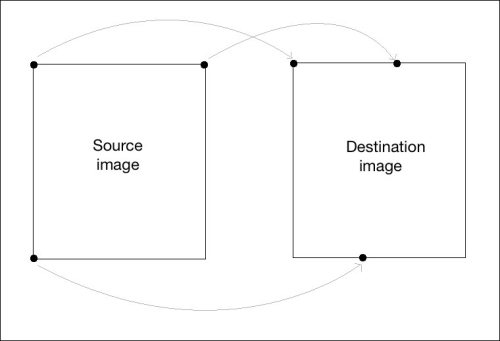
\includegraphics[width=0.6\columnwidth]{figures/Fig25.png}
	\caption{Affine Transformation}
	\label{fig25}
\end{figure}

To get the transformation matrix, we have a function called \textbf{getAffineTransform} in OpenCV. Once we have the affine 	transformation matrix, we use the \textbf{warpAffine} function to apply this matrix to the input image. We can also get the 	mirror image of the input image. We just need to change the control points in the following way:

\vspace{0.5cm}

\begin{tcolorbox}[breakable, size=fbox, boxrule=1pt, pad at break*=1mm,colback=cellbackground, colframe=cellborder]
	\prompt{In}{incolor}{ }{\boxspacing}
	\begin{Verbatim}[commandchars=\\\{\}]
\PY{k+kn}{import} \PY{n+nn}{cv2}
\PY{k+kn}{import} \PY{n+nn}{numpy} \PY{k}{as} \PY{n+nn}{np}
\PY{k+kn}{import} \PY{n+nn}{matplotlib}\PY{n+nn}{.}\PY{n+nn}{pyplot} \PY{k}{as} \PY{n+nn}{plt}
	\end{Verbatim}
\end{tcolorbox}

\begin{tcolorbox}[breakable, size=fbox, boxrule=1pt, pad at break*=1mm,colback=cellbackground, colframe=cellborder]
	\prompt{In}{incolor}{ }{\boxspacing}
	\begin{Verbatim}[commandchars=\\\{\}]
\PY{n}{img} \PY{o}{=} \PY{n}{cv2}\PY{o}{.}\PY{n}{imread}\PY{p}{(}\PY{l+s+s1}{\PYZsq{}}\PY{l+s+s1}{images/Sample7.jpg}\PY{l+s+s1}{\PYZsq{}}\PY{p}{)}
\PY{n}{rows}\PY{p}{,} \PY{n}{cols} \PY{o}{=} \PY{n}{img}\PY{o}{.}\PY{n}{shape}\PY{p}{[}\PY{p}{:}\PY{l+m+mi}{2}\PY{p}{]}
		
\PY{n+nb}{print}\PY{p}{(}\PY{l+s+s1}{\PYZsq{}}\PY{l+s+s1}{rows : }\PY{l+s+si}{\PYZob{}\PYZcb{}}\PY{l+s+s1}{\PYZsq{}}\PY{o}{.}\PY{n}{format}\PY{p}{(}\PY{n}{rows}\PY{p}{)}\PY{p}{)}
\PY{n+nb}{print}\PY{p}{(}\PY{l+s+s1}{\PYZsq{}}\PY{l+s+s1}{columns : }\PY{l+s+si}{\PYZob{}\PYZcb{}}\PY{l+s+s1}{\PYZsq{}}\PY{o}{.}\PY{n}{format}\PY{p}{(}\PY{n}{cols}\PY{p}{)}\PY{p}{)}
	\end{Verbatim}
\end{tcolorbox}

\begin{Verbatim}[commandchars=\\\{\}]
rows : 299
columns : 299
\end{Verbatim}


\begin{tcolorbox}[breakable, size=fbox, boxrule=1pt, pad at break*=1mm,colback=cellbackground, colframe=cellborder]
	\prompt{In}{incolor}{ }{\boxspacing}
	\begin{Verbatim}[commandchars=\\\{\}]
\PY{n}{src\PYZus{}points} \PY{o}{=} \PY{n}{np}\PY{o}{.}\PY{n}{float32}\PY{p}{(}\PY{p}{[}\PY{p}{[}\PY{l+m+mi}{0}\PY{p}{,}\PY{l+m+mi}{0}\PY{p}{]}\PY{p}{,} \PY{p}{[}\PY{n}{cols}\PY{o}{\PYZhy{}}\PY{l+m+mi}{1}\PY{p}{,}\PY{l+m+mi}{0}\PY{p}{]}\PY{p}{,} \PY{p}{[}\PY{l+m+mi}{0}\PY{p}{,}\PY{n}{rows}\PY{o}{\PYZhy{}}\PY{l+m+mi}{1}\PY{p}{]}\PY{p}{]}\PY{p}{)}
\PY{n}{dst\PYZus{}points} \PY{o}{=} \PY{n}{np}\PY{o}{.}\PY{n}{float32}\PY{p}{(}\PY{p}{[}\PY{p}{[}\PY{n}{cols}\PY{o}{\PYZhy{}}\PY{l+m+mi}{1}\PY{p}{,}\PY{l+m+mi}{0}\PY{p}{]}\PY{p}{,} \PY{p}{[}\PY{l+m+mi}{0}\PY{p}{,}\PY{l+m+mi}{0}\PY{p}{]}\PY{p}{,} \PY{p}{[}\PY{n}{cols}\PY{o}{\PYZhy{}}\PY{l+m+mi}{1}\PY{p}{,}\PY{n}{rows}\PY{o}{\PYZhy{}}\PY{l+m+mi}{1}\PY{p}{]}\PY{p}{]}\PY{p}{)}

\PY{n+nb}{print}\PY{p}{(}\PY{l+s+s1}{\PYZsq{}}\PY{l+s+s1}{Source points:}\PY{l+s+se}{\PYZbs{}n}\PY{l+s+s1}{ }\PY{l+s+si}{\PYZob{}\PYZcb{}}\PY{l+s+s1}{\PYZsq{}}\PY{o}{.}\PY{n}{format}\PY{p}{(}\PY{n}{src\PYZus{}points}\PY{p}{)}\PY{p}{)}
\PY{n+nb}{print}\PY{p}{(}\PY{l+s+s1}{\PYZsq{}}\PY{l+s+s1}{Destination Points:}\PY{l+s+se}{\PYZbs{}n}\PY{l+s+s1}{ }\PY{l+s+si}{\PYZob{}\PYZcb{}}\PY{l+s+s1}{\PYZsq{}}\PY{o}{.}\PY{n}{format}\PY{p}{(}\PY{n}{dst\PYZus{}points}\PY{p}{)}\PY{p}{)}
	\end{Verbatim}
\end{tcolorbox}

\begin{Verbatim}[commandchars=\\\{\}]
Source points:
[  0.   0.]
[298.   0.]
[  0. 298.]
Destination Points:
[298.   0.]
[  0.   0.]
[298. 298.]
\end{Verbatim}

\begin{tcolorbox}[breakable, size=fbox, boxrule=1pt, pad at break*=1mm,colback=cellbackground, colframe=cellborder]
	\prompt{In}{incolor}{ }{\boxspacing}
	\begin{Verbatim}[commandchars=\\\{\}]
\PY{n}{affine\PYZus{}matrix} \PY{o}{=} \PY{n}{cv2}\PY{o}{.}\PY{n}{getAffineTransform}\PY{p}{(}\PY{n}{src\PYZus{}points}\PY{p}{,} \PY{n}{dst\PYZus{}points}\PY{p}{)}
\PY{n}{img\PYZus{}output} \PY{o}{=} \PY{n}{cv2}\PY{o}{.}\PY{n}{warpAffine}\PY{p}{(}\PY{n}{img}\PY{p}{,} \PY{n}{affine\PYZus{}matrix}\PY{p}{,} \PY{p}{(}\PY{n}{cols}\PY{p}{,}\PY{n}{rows}\PY{p}{)}\PY{p}{)}
	\end{Verbatim}
\end{tcolorbox}

\begin{tcolorbox}[breakable, size=fbox, boxrule=1pt, pad at break*=1mm,colback=cellbackground, colframe=cellborder]
	\prompt{In}{incolor}{ }{\boxspacing}
	\begin{Verbatim}[commandchars=\\\{\}]
\PY{n}{fig}\PY{p}{,} \PY{n}{axs} \PY{o}{=} \PY{n}{plt}\PY{o}{.}\PY{n}{subplots}\PY{p}{(}\PY{l+m+mi}{1}\PY{p}{,}\PY{l+m+mi}{2}\PY{p}{,}\PY{n}{figsize}\PY{o}{=}\PY{p}{(}\PY{l+m+mi}{10}\PY{p}{,}\PY{l+m+mi}{5}\PY{p}{)}\PY{p}{)}

\PY{n}{axs}\PY{p}{[}\PY{l+m+mi}{0}\PY{p}{]}\PY{o}{.}\PY{n}{imshow}\PY{p}{(}\PY{n}{img}\PY{p}{)}
\PY{n}{axs}\PY{p}{[}\PY{l+m+mi}{0}\PY{p}{]}\PY{o}{.}\PY{n}{set\PYZus{}title}\PY{p}{(}\PY{l+s+s1}{\PYZsq{}}\PY{l+s+s1}{Input}\PY{l+s+s1}{\PYZsq{}}\PY{p}{)}
\PY{n}{axs}\PY{p}{[}\PY{l+m+mi}{1}\PY{p}{]}\PY{o}{.}\PY{n}{imshow}\PY{p}{(}\PY{n}{img\PYZus{}output}\PY{p}{)}
\PY{n}{axs}\PY{p}{[}\PY{l+m+mi}{1}\PY{p}{]}\PY{o}{.}\PY{n}{set\PYZus{}title}\PY{p}{(}\PY{l+s+s1}{\PYZsq{}}\PY{l+s+s1}{Output}\PY{l+s+s1}{\PYZsq{}}\PY{p}{)}
	\end{Verbatim}
\end{tcolorbox}

\begin{tcolorbox}[breakable, size=fbox, boxrule=.5pt, pad at break*=1mm, opacityfill=0]
	\prompt{Out}{outcolor}{ }{\boxspacing}
	\begin{Verbatim}[commandchars=\\\{\}]
Text(0.5, 1.0, 'Output')
	\end{Verbatim}
\end{tcolorbox}

\begin{center}
	\adjustimage{max size={0.9\linewidth}{0.9\paperheight}}{figures/p9.png}
\end{center}
{ \hspace*{\fill} \\}

Here, the mapping looks something like this(Figure \ref{fig26}):

\begin{figure}[H]
	%\resizebox{\linewidth}{!}{
	\centering 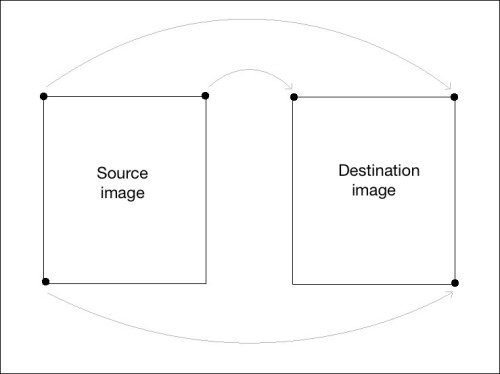
\includegraphics[width=0.6\columnwidth]{figures/Fig26.jpg}
	\caption{Affine Transformation}
	\label{fig26}
\end{figure}

\subsection{Projective Transformations}
Affine transformations are useful, but they impose certain restrictions. A projective transformation, on the other hand, gives us more freedom. It is also referred to as \textbf{homography}. In order to understand projective transformations, we need to understand how projective geometry works. We basically describe what happens to an image when the point of view is changed. For example, if you are standing right in front of a sheet of paper with a square drawn on it, it will look like a square. Now, if you start tilting that sheet of paper, the square will start looking more and more like a trapezoid. Projective transformations allow us to capture this dynamic in a nice mathematical way. These transformations preserve neither sizes nor angles, but they do preserve incidence and cross-ratio.

We can say that any two images on a given plane are related by a homography. As long as they are in the same plane, we can transform anything into anything else. This has many practical applications such as augmented reality, image rectification, image registration, or the computation of camera motion between two images. Once the camera rotation and translation have been extracted from an estimated homography matrix, this information may be used for navigation, or to insert models of 3D objects into an image or video. This way, they are rendered with the correct perspective and it will look like they were part of the original scene.

\vspace{0.5cm}

 \begin{tcolorbox}[breakable, size=fbox, boxrule=1pt, pad at break*=1mm,colback=cellbackground, colframe=cellborder]
	\prompt{In}{incolor}{ }{\boxspacing}
	\begin{Verbatim}[commandchars=\\\{\}]
\PY{k+kn}{import} \PY{n+nn}{cv2}
\PY{k+kn}{import} \PY{n+nn}{numpy} \PY{k}{as} \PY{n+nn}{np}
\PY{k+kn}{import} \PY{n+nn}{matplotlib}\PY{n+nn}{.}\PY{n+nn}{pyplot} \PY{k}{as} \PY{n+nn}{plt}
	\end{Verbatim}
\end{tcolorbox}

\begin{tcolorbox}[breakable, size=fbox, boxrule=1pt, pad at break*=1mm,colback=cellbackground, colframe=cellborder]
	\prompt{In}{incolor}{ }{\boxspacing}
	\begin{Verbatim}[commandchars=\\\{\}]
\PY{n}{img} \PY{o}{=} \PY{n}{cv2}\PY{o}{.}\PY{n}{imread}\PY{p}{(}\PY{l+s+s1}{\PYZsq{}}\PY{l+s+s1}{images/Sample8.jpg}\PY{l+s+s1}{\PYZsq{}}\PY{p}{)}
\PY{n}{rows}\PY{p}{,} \PY{n}{cols} \PY{o}{=} \PY{n}{img}\PY{o}{.}\PY{n}{shape}\PY{p}{[}\PY{p}{:}\PY{l+m+mi}{2}\PY{p}{]}

\PY{n+nb}{print}\PY{p}{(}\PY{l+s+s1}{\PYZsq{}}\PY{l+s+s1}{Rows: }\PY{l+s+si}{\PYZob{}\PYZcb{}}\PY{l+s+s1}{\PYZsq{}}\PY{o}{.}\PY{n}{format}\PY{p}{(}\PY{n}{rows}\PY{p}{)}\PY{p}{)}
\PY{n+nb}{print}\PY{p}{(}\PY{l+s+s1}{\PYZsq{}}\PY{l+s+s1}{Columns: }\PY{l+s+si}{\PYZob{}\PYZcb{}}\PY{l+s+s1}{\PYZsq{}}\PY{o}{.}\PY{n}{format}\PY{p}{(}\PY{n}{cols}\PY{p}{)}\PY{p}{)}
	\end{Verbatim}
\end{tcolorbox}

 \begin{Verbatim}[commandchars=\\\{\}]
Rows: 638
Columns: 750
\end{Verbatim}

\begin{tcolorbox}[breakable, size=fbox, boxrule=1pt, pad at break*=1mm,colback=cellbackground, colframe=cellborder]
	\prompt{In}{incolor}{ }{\boxspacing}
	\begin{Verbatim}[commandchars=\\\{\}]
\PY{n}{src\PYZus{}points} \PY{o}{=} \PY{n}{np}\PY{o}{.}\PY{n}{float32}\PY{p}{(}\PY{p}{[}\PY{p}{[}\PY{l+m+mi}{0}\PY{p}{,}\PY{l+m+mi}{0}\PY{p}{]}\PY{p}{,} \PY{p}{[}\PY{n}{cols}\PY{o}{\PYZhy{}}\PY{l+m+mi}{1}\PY{p}{,}\PY{l+m+mi}{0}\PY{p}{]}\PY{p}{,} \PY{p}{[}\PY{l+m+mi}{0}\PY{p}{,}\PY{n}{rows}\PY{o}{\PYZhy{}}\PY{l+m+mi}{1}\PY{p}{]}\PY{p}{,}
\PY{p}{[}\PY{n}{cols}\PY{o}{\PYZhy{}}\PY{l+m+mi}{1}\PY{p}{,}\PY{n}{rows}\PY{o}{\PYZhy{}}\PY{l+m+mi}{1}\PY{p}{]}\PY{p}{]}\PY{p}{)}
\PY{n}{dst\PYZus{}points} \PY{o}{=} \PY{n}{np}\PY{o}{.}\PY{n}{float32}\PY{p}{(}\PY{p}{[}\PY{p}{[}\PY{l+m+mi}{0}\PY{p}{,}\PY{l+m+mi}{0}\PY{p}{]}\PY{p}{,} \PY{p}{[}\PY{n}{cols}\PY{o}{\PYZhy{}}\PY{l+m+mi}{1}\PY{p}{,}\PY{l+m+mi}{0}\PY{p}{]}\PY{p}{,} \PY{p}{[}\PY{n+nb}{int}\PY{p}{(}\PY{l+m+mf}{0.33}\PY{o}{*}\PY{n}{cols}\PY{p}{)}\PY{p}{,}\PY{n}{rows}\PY{o}{\PYZhy{}}\PY{l+m+mi}{1}\PY{p}{]}\PY{p}{,}
\PY{p}{[}\PY{n+nb}{int}\PY{p}{(}\PY{l+m+mf}{0.66}\PY{o}{*}\PY{n}{cols}\PY{p}{)}\PY{p}{,}\PY{n}{rows}\PY{o}{\PYZhy{}}\PY{l+m+mi}{1}\PY{p}{]}\PY{p}{]}\PY{p}{)} 

\PY{n+nb}{print}\PY{p}{(}\PY{l+s+s1}{\PYZsq{}}\PY{l+s+s1}{Source points:}\PY{l+s+se}{\PYZbs{}n}\PY{l+s+s1}{ }\PY{l+s+si}{\PYZob{}\PYZcb{}}\PY{l+s+s1}{\PYZsq{}}\PY{o}{.}\PY{n}{format}\PY{p}{(}\PY{n}{src\PYZus{}points}\PY{p}{)}\PY{p}{)}
\PY{n+nb}{print}\PY{p}{(}\PY{l+s+s1}{\PYZsq{}}\PY{l+s+s1}{Destination points:}\PY{l+s+se}{\PYZbs{}n}\PY{l+s+s1}{ }\PY{l+s+si}{\PYZob{}\PYZcb{}}\PY{l+s+s1}{\PYZsq{}}\PY{o}{.}\PY{n}{format}\PY{p}{(}\PY{n}{dst\PYZus{}points}\PY{p}{)}\PY{p}{)}
	\end{Verbatim}
\end{tcolorbox}

\begin{Verbatim}[commandchars=\\\{\}]
Source points:
[  0.   0.]
[749.   0.]
[  0. 637.]
[749. 637.]
Destination points:
[  0.   0.]
[749.   0.]
[247. 637.]
[495. 637.]
\end{Verbatim}

\begin{tcolorbox}[breakable, size=fbox, boxrule=1pt, pad at break*=1mm,colback=cellbackground, colframe=cellborder]
	\prompt{In}{incolor}{ }{\boxspacing}
	\begin{Verbatim}[commandchars=\\\{\}]
\PY{n}{projective\PYZus{}matrix} \PY{o}{=} \PY{n}{cv2}\PY{o}{.}\PY{n}{getPerspectiveTransform}\PY{p}{(}\PY{n}{src\PYZus{}points}\PY{p}{,} \PY{n}{dst\PYZus{}points}\PY{p}{)}
\PY{n}{img\PYZus{}output} \PY{o}{=} \PY{n}{cv2}\PY{o}{.}\PY{n}{warpPerspective}\PY{p}{(}\PY{n}{img}\PY{p}{,} \PY{n}{projective\PYZus{}matrix}\PY{p}{,} \PY{p}{(}\PY{n}{cols}\PY{p}{,}\PY{n}{rows}\PY{p}{)}\PY{p}{)}
	\end{Verbatim}
\end{tcolorbox}
\vspace{0.5cm}
\begin{tcolorbox}[breakable, size=fbox, boxrule=1pt, pad at break*=1mm,colback=cellbackground, colframe=cellborder]
	\prompt{In}{incolor}{ }{\boxspacing}
	\begin{Verbatim}[commandchars=\\\{\}]
\PY{n}{fig}\PY{p}{,} \PY{n}{axs} \PY{o}{=} \PY{n}{plt}\PY{o}{.}\PY{n}{subplots}\PY{p}{(}\PY{l+m+mi}{1}\PY{p}{,}\PY{l+m+mi}{2}\PY{p}{,}\PY{n}{figsize}\PY{o}{=}\PY{p}{(}\PY{l+m+mi}{10}\PY{p}{,}\PY{l+m+mi}{5}\PY{p}{)}\PY{p}{)}

\PY{n}{axs}\PY{p}{[}\PY{l+m+mi}{0}\PY{p}{]}\PY{o}{.}\PY{n}{imshow}\PY{p}{(}\PY{n}{img}\PY{p}{)}
\PY{n}{axs}\PY{p}{[}\PY{l+m+mi}{0}\PY{p}{]}\PY{o}{.}\PY{n}{set\PYZus{}title}\PY{p}{(}\PY{l+s+s1}{\PYZsq{}}\PY{l+s+s1}{Input}\PY{l+s+s1}{\PYZsq{}}\PY{p}{)}
\PY{n}{axs}\PY{p}{[}\PY{l+m+mi}{1}\PY{p}{]}\PY{o}{.}\PY{n}{imshow}\PY{p}{(}\PY{n}{img\PYZus{}output}\PY{p}{)}
\PY{n}{axs}\PY{p}{[}\PY{l+m+mi}{1}\PY{p}{]}\PY{o}{.}\PY{n}{set\PYZus{}title}\PY{p}{(}\PY{l+s+s1}{\PYZsq{}}\PY{l+s+s1}{Output}\PY{l+s+s1}{\PYZsq{}}\PY{p}{)}
	\end{Verbatim}
\end{tcolorbox}

\begin{tcolorbox}[breakable, size=fbox, boxrule=.5pt, pad at break*=1mm, opacityfill=0]
\prompt{Out}{outcolor}{ }{\boxspacing}
\begin{Verbatim}[commandchars=\\\{\}]
Text(0.5, 1.0, 'Output')
\end{Verbatim}
\end{tcolorbox}

\begin{center}
	\adjustimage{max size={0.9\linewidth}{0.9\paperheight}}{figures/p10.png}
\end{center}
{ \hspace*{\fill} \\}

We can choose four control points in the source image and map them to the destination image. Parallel lines will not remain parallel lines after the transformation. We use a function called \textbf{getPerspectiveTransform} to get the transformation matrix.


\section{Image Filters}

In this section, we will learn how to use fundamental image processing operators. We are going to discuss edge detection and how we can use image filters to apply various effects on photos.

\subsection{2D Convolution}
Convolution is a fundamental operation in image processing. We basically apply a mathematical operator to each pixel and change its value in some way. To apply this mathematical operator, we use another matrix called a kernel. The kernel is usually much smaller in size than the input image. For each pixel in the image, we take the kernel and place it on top such that the center of the kernel coincides with the pixel under consideration. We then multiply each value in the kernel matrix with the corresponding values in the image, and then sum it up. This is the new value that will be substituted in this position in the output image.

Here, the kernel is called the \textbf{image filter} and the process of applying this kernel to the given image is called \textbf{image filtering}. The output obtained after applying the kernel to the image is called the filtered image. Depending on the values in the kernel, it performs different functions like blurring, detecting edges, and so on. Figure \ref{fig27} should help you visualize the image filtering operation:

\begin{figure}[H]
	%\resizebox{\linewidth}{!}{
	\centering 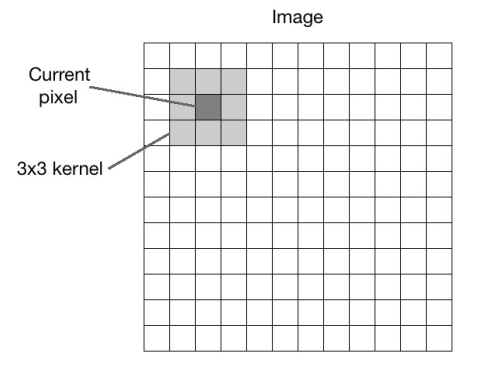
\includegraphics[width=0.6\columnwidth]{figures/Fig27.png}
	\caption{Image Kernel}
	\label{fig27}
\end{figure}

Let's start with the simplest case which is identity kernel. This kernel doesn't really change the input image. If we consider a 3$\times$3 identity kernel, it looks something like the following:

\begin{center}
	\[
	\textit{I} =  
	\begin{bmatrix}
		0 & 0 & 0 \\
		0 & 1 & 0 \\
		0 & 0 & 0
	\end{bmatrix}
	\]
\end{center}

\subsection{Blurring}
Blurring refers to averaging the pixel values within a neighborhood. This is also called a \textbf{low pass filter}. A low pass filter is a filter that allows low frequencies and blocks higher frequencies. Frequency refers to the rate of change of pixel values. So we can say that the sharp edges would be high frequency content because the pixel values change rapidly in that region. Going by that logic, plain areas would be low frequency content. Going by this definition, a low pass filter would try to smoothen the edges.

A simple way to build a low pass filter is by uniformly averaging the values in the neighborhood of a pixel. We can choose the size of the kernel depending on how much we want to smoothen the image, and it will correspondingly have different effects. If you choose a bigger size, then you will be averaging over a larger area. This tends to increase the smoothening effect. A 3$\times$3 low pass filter kernel looks like the following:

\begin{center}
	\[
	\textit{I} = \frac{1}{9}  
	\begin{bmatrix}
		1 & 1 & 1 \\
		1 & 1 & 1 \\
		1 & 1 & 1
	\end{bmatrix}
	\]
\end{center}

We are dividing the matrix by 9 because we want the values to sum up to 1. This is called \textbf{normalization}, and it's important because we don't want to artificially increase the intensity value at that pixel's location. So you should normalize the kernel before applying it to an image. Here is the code to apply this low pass filter to an image:

\vspace{0.5cm}

\begin{tcolorbox}[breakable, size=fbox, boxrule=1pt, pad at break*=1mm,colback=cellbackground, colframe=cellborder]
	\prompt{In}{incolor}{ }{\boxspacing}
	\begin{Verbatim}[commandchars=\\\{\}]
\PY{k+kn}{import} \PY{n+nn}{cv2}
\PY{k+kn}{import} \PY{n+nn}{numpy} \PY{k}{as} \PY{n+nn}{np}
\PY{k+kn}{import} \PY{n+nn}{matplotlib}\PY{n+nn}{.}\PY{n+nn}{pyplot} \PY{k}{as} \PY{n+nn}{plt}
	\end{Verbatim}
\end{tcolorbox}

\begin{tcolorbox}[breakable, size=fbox, boxrule=1pt, pad at break*=1mm,colback=cellbackground, colframe=cellborder]
	\prompt{In}{incolor}{ }{\boxspacing}
	\begin{Verbatim}[commandchars=\\\{\}]
\PY{n}{img} \PY{o}{=} \PY{n}{cv2}\PY{o}{.}\PY{n}{imread}\PY{p}{(}\PY{l+s+s1}{\PYZsq{}}\PY{l+s+s1}{images/Sample9.jpg}\PY{l+s+s1}{\PYZsq{}}\PY{p}{)}
\PY{n}{rows}\PY{p}{,} \PY{n}{cols} \PY{o}{=} \PY{n}{img}\PY{o}{.}\PY{n}{shape}\PY{p}{[}\PY{p}{:}\PY{l+m+mi}{2}\PY{p}{]}

\PY{n+nb}{print}\PY{p}{(}\PY{l+s+s1}{\PYZsq{}}\PY{l+s+s1}{Rows: }\PY{l+s+si}{\PYZob{}\PYZcb{}}\PY{l+s+s1}{\PYZsq{}}\PY{o}{.}\PY{n}{format}\PY{p}{(}\PY{n}{rows}\PY{p}{)}\PY{p}{)}
\PY{n+nb}{print}\PY{p}{(}\PY{l+s+s1}{\PYZsq{}}\PY{l+s+s1}{Columns: }\PY{l+s+si}{\PYZob{}\PYZcb{}}\PY{l+s+s1}{\PYZsq{}}\PY{o}{.}\PY{n}{format}\PY{p}{(}\PY{n}{cols}\PY{p}{)}\PY{p}{)}
	\end{Verbatim}
\end{tcolorbox}

\begin{Verbatim}[commandchars=\\\{\}]
Rows: 765
Columns: 637
\end{Verbatim}

\begin{tcolorbox}[breakable, size=fbox, boxrule=1pt, pad at break*=1mm,colback=cellbackground, colframe=cellborder]
	\prompt{In}{incolor}{ }{\boxspacing}
	\begin{Verbatim}[commandchars=\\\{\}]
\PY{c+c1}{\PYZsh{} Create Kernels}
\PY{n}{kernel\PYZus{}identity} \PY{o}{=} \PY{n}{np}\PY{o}{.}\PY{n}{array}\PY{p}{(}\PY{p}{[}\PY{p}{[}\PY{l+m+mi}{0}\PY{p}{,}\PY{l+m+mi}{0}\PY{p}{,}\PY{l+m+mi}{0}\PY{p}{]}\PY{p}{,} \PY{p}{[}\PY{l+m+mi}{0}\PY{p}{,}\PY{l+m+mi}{1}\PY{p}{,}\PY{l+m+mi}{0}\PY{p}{]}\PY{p}{,} \PY{p}{[}\PY{l+m+mi}{0}\PY{p}{,}\PY{l+m+mi}{0}\PY{p}{,}\PY{l+m+mi}{0}\PY{p}{]}\PY{p}{]}\PY{p}{)}
\PY{n}{kernel\PYZus{}5x5} \PY{o}{=} \PY{n}{np}\PY{o}{.}\PY{n}{ones}\PY{p}{(}\PY{p}{(}\PY{l+m+mi}{5}\PY{p}{,}\PY{l+m+mi}{5}\PY{p}{)}\PY{p}{,} \PY{n}{np}\PY{o}{.}\PY{n}{float32}\PY{p}{)} \PY{o}{/} \PY{l+m+mf}{25.0}
\PY{n}{kernel\PYZus{}9x9} \PY{o}{=} \PY{n}{np}\PY{o}{.}\PY{n}{ones}\PY{p}{(}\PY{p}{(}\PY{l+m+mi}{9}\PY{p}{,}\PY{l+m+mi}{9}\PY{p}{)}\PY{p}{,} \PY{n}{np}\PY{o}{.}\PY{n}{float32}\PY{p}{)} \PY{o}{/} \PY{l+m+mf}{81.0}
	\end{Verbatim}
\end{tcolorbox}

\begin{tcolorbox}[breakable, size=fbox, boxrule=1pt, pad at break*=1mm,colback=cellbackground, colframe=cellborder]
	\prompt{In}{incolor}{ }{\boxspacing}
	\begin{Verbatim}[commandchars=\\\{\}]
\PY{c+c1}{\PYZsh{} Apply Kernels}
\PY{n}{identity\PYZus{}img} \PY{o}{=} \PY{n}{cv2}\PY{o}{.}\PY{n}{filter2D}\PY{p}{(}\PY{n}{img}\PY{p}{,} \PY{o}{\PYZhy{}}\PY{l+m+mi}{1}\PY{p}{,} \PY{n}{kernel\PYZus{}identity}\PY{p}{)}
\PY{n}{kernel\PYZus{}5x5\PYZus{}img} \PY{o}{=} \PY{n}{cv2}\PY{o}{.}\PY{n}{filter2D}\PY{p}{(}\PY{n}{img}\PY{p}{,} \PY{o}{\PYZhy{}}\PY{l+m+mi}{1}\PY{p}{,} \PY{n}{kernel\PYZus{}5x5}\PY{p}{)}
\PY{n}{kernel\PYZus{}9x9\PYZus{}img} \PY{o}{=} \PY{n}{cv2}\PY{o}{.}\PY{n}{filter2D}\PY{p}{(}\PY{n}{img}\PY{p}{,} \PY{o}{\PYZhy{}}\PY{l+m+mi}{1}\PY{p}{,} \PY{n}{kernel\PYZus{}9x9}\PY{p}{)}
	\end{Verbatim}
\end{tcolorbox}

\begin{tcolorbox}[breakable, size=fbox, boxrule=1pt, pad at break*=1mm,colback=cellbackground, colframe=cellborder]
	\prompt{In}{incolor}{ }{\boxspacing}
	\begin{Verbatim}[commandchars=\\\{\}]
\PY{n}{fig}\PY{p}{,} \PY{n}{axs} \PY{o}{=} \PY{n}{plt}\PY{o}{.}\PY{n}{subplots}\PY{p}{(}\PY{l+m+mi}{2}\PY{p}{,}\PY{l+m+mi}{2}\PY{p}{,}\PY{n}{figsize}\PY{o}{=}\PY{p}{(}\PY{l+m+mi}{10}\PY{p}{,}\PY{l+m+mi}{10}\PY{p}{)}\PY{p}{)}

\PY{n}{axs}\PY{p}{[}\PY{l+m+mi}{0}\PY{p}{,}\PY{l+m+mi}{0}\PY{p}{]}\PY{o}{.}\PY{n}{imshow}\PY{p}{(}\PY{n}{img}\PY{p}{)}
\PY{n}{axs}\PY{p}{[}\PY{l+m+mi}{0}\PY{p}{,}\PY{l+m+mi}{0}\PY{p}{]}\PY{o}{.}\PY{n}{set\PYZus{}title}\PY{p}{(}\PY{l+s+s1}{\PYZsq{}}\PY{l+s+s1}{Input}\PY{l+s+s1}{\PYZsq{}}\PY{p}{)}

\PY{n}{axs}\PY{p}{[}\PY{l+m+mi}{0}\PY{p}{,}\PY{l+m+mi}{1}\PY{p}{]}\PY{o}{.}\PY{n}{imshow}\PY{p}{(}\PY{n}{identity\PYZus{}img}\PY{p}{)}
\PY{n}{axs}\PY{p}{[}\PY{l+m+mi}{0}\PY{p}{,}\PY{l+m+mi}{1}\PY{p}{]}\PY{o}{.}\PY{n}{set\PYZus{}title}\PY{p}{(}\PY{l+s+s1}{\PYZsq{}}\PY{l+s+s1}{identity kernel}\PY{l+s+s1}{\PYZsq{}}\PY{p}{)}

\PY{n}{axs}\PY{p}{[}\PY{l+m+mi}{1}\PY{p}{,}\PY{l+m+mi}{0}\PY{p}{]}\PY{o}{.}\PY{n}{imshow}\PY{p}{(}\PY{n}{kernel\PYZus{}5x5\PYZus{}img}\PY{p}{)}
\PY{n}{axs}\PY{p}{[}\PY{l+m+mi}{1}\PY{p}{,}\PY{l+m+mi}{0}\PY{p}{]}\PY{o}{.}\PY{n}{set\PYZus{}title}\PY{p}{(}\PY{l+s+s1}{\PYZsq{}}\PY{l+s+s1}{5x5 kernel}\PY{l+s+s1}{\PYZsq{}}\PY{p}{)}

\PY{n}{axs}\PY{p}{[}\PY{l+m+mi}{1}\PY{p}{,}\PY{l+m+mi}{1}\PY{p}{]}\PY{o}{.}\PY{n}{imshow}\PY{p}{(}\PY{n}{kernel\PYZus{}9x9\PYZus{}img}\PY{p}{)}
\PY{n}{axs}\PY{p}{[}\PY{l+m+mi}{1}\PY{p}{,}\PY{l+m+mi}{1}\PY{p}{]}\PY{o}{.}\PY{n}{set\PYZus{}title}\PY{p}{(}\PY{l+s+s1}{\PYZsq{}}\PY{l+s+s1}{9x9 kernel}\PY{l+s+s1}{\PYZsq{}}\PY{p}{)}
	\end{Verbatim}
\end{tcolorbox}

\begin{tcolorbox}[breakable, size=fbox, boxrule=.5pt, pad at break*=1mm, opacityfill=0]
	\prompt{Out}{outcolor}{ }{\boxspacing}
	\begin{Verbatim}[commandchars=\\\{\}]
Text(0.5, 1.0, '9x9 kernel')
	\end{Verbatim}
\end{tcolorbox}

\begin{center}
	\adjustimage{max size={0.9\linewidth}{0.9\paperheight}}{figures/p11.png}
\end{center}
{ \hspace*{\fill} \\}

In the preceding code, we are generating different kernels in the code which are kernel\_identity, kernel\_5$\times$5, and kernel\_9$\times$9. We use the function, \textbf{filter2D}, to apply these kernels to the input image. If you look at the images carefully, you can see that they keep getting blurrier as we increase the kernel size. The reason for this is because when we increase the kernel size, we are averaging over a larger area. This tends to have a larger blurring effect. An alternative way of doing this would be by using the OpenCV function, \textbf{cv2.blur}. If you don't want to generate the kernels yourself, you can just use this function directly.

\section{Edge Detection}
The process of edge detection involves detecting sharp edges in the image and producing a binary image as the output. Typically, we draw white lines on a black background to indicate those edges. We can think of edge detection as a high pass filtering operation. A high pass filter allows high frequency content to pass through and blocks the low frequency content. As we discussed earlier, edges are high frequency content. In edge detection, we want to retain these edges and discard everything else. Hence, we should build a kernel that is the equivalent of a high pass filter.

Let's start with a simple edge detection filter known as the Sobel filter. Since edges can occur in both horizontal and vertical directions, the \textbf{Sobel filter} is composed of the following two kernels:

\begin{center}
	\[
	\textit{$S_x$} =  
	\begin{bmatrix}
		-1 & 0 & 1 \\
		-2 & 1 & 2 \\
		-1 & 0 & 1
	\end{bmatrix}
	\]
	\hspace{2cm}
	\[
	\textit{$S_y$} =  
	\begin{bmatrix}
		-1 & -2 & -1 \\
		0 & 0 & 0 \\
		1 & 2 & 1
	\end{bmatrix}
	\]
\end{center}

The kernel on the left detects horizontal edges and the kernel on the right detects vertical edges. OpenCV provides a function to directly apply the Sobel filter to a given image.

\vspace{0.5cm}

\begin{tcolorbox}[breakable, size=fbox, boxrule=1pt, pad at break*=1mm,colback=cellbackground, colframe=cellborder]
	\prompt{In}{incolor}{ }{\boxspacing}
	\begin{Verbatim}[commandchars=\\\{\}]
\PY{k+kn}{import} \PY{n+nn}{cv2}
\PY{k+kn}{import} \PY{n+nn}{numpy} \PY{k}{as} \PY{n+nn}{np}
\PY{k+kn}{import} \PY{n+nn}{matplotlib}\PY{n+nn}{.}\PY{n+nn}{pyplot} \PY{k}{as} \PY{n+nn}{plt}
	\end{Verbatim}
\end{tcolorbox}

\begin{tcolorbox}[breakable, size=fbox, boxrule=1pt, pad at break*=1mm,colback=cellbackground, colframe=cellborder]
	\prompt{In}{incolor}{10}{\boxspacing}
	\begin{Verbatim}[commandchars=\\\{\}]
\PY{n}{img} \PY{o}{=} \PY{n}{cv2}\PY{o}{.}\PY{n}{imread}\PY{p}{(}\PY{l+s+s1}{\PYZsq{}}\PY{l+s+s1}{images/Sample10.jpg}\PY{l+s+s1}{\PYZsq{}}\PY{p}{)}
\PY{n}{rows}\PY{p}{,} \PY{n}{cols}\PY{p}{,} \PY{n}{\PYZus{}} \PY{o}{=} \PY{n}{img}\PY{o}{.}\PY{n}{shape}

\PY{n+nb}{print}\PY{p}{(}\PY{l+s+s1}{\PYZsq{}}\PY{l+s+s1}{Rows: }\PY{l+s+si}{\PYZob{}\PYZcb{}}\PY{l+s+s1}{\PYZsq{}}\PY{o}{.}\PY{n}{format}\PY{p}{(}\PY{n}{rows}\PY{p}{)}\PY{p}{)}
\PY{n+nb}{print}\PY{p}{(}\PY{l+s+s1}{\PYZsq{}}\PY{l+s+s1}{Columns: }\PY{l+s+si}{\PYZob{}\PYZcb{}}\PY{l+s+s1}{\PYZsq{}}\PY{o}{.}\PY{n}{format}\PY{p}{(}\PY{n}{cols}\PY{p}{)}\PY{p}{)}
	\end{Verbatim}
\end{tcolorbox}

\begin{Verbatim}[commandchars=\\\{\}]
Rows: 212
Columns: 220
\end{Verbatim}

\begin{tcolorbox}[breakable, size=fbox, boxrule=1pt, pad at break*=1mm,colback=cellbackground, colframe=cellborder]
	\prompt{In}{incolor}{ }{\boxspacing}
	\begin{Verbatim}[commandchars=\\\{\}]
\PY{c+c1}{\PYZsh{} iameg resizing}
\PY{n}{img} \PY{o}{=} \PY{n}{cv2}\PY{o}{.}\PY{n}{resize}\PY{p}{(}\PY{n}{img}\PY{p}{,}\PY{p}{(}\PY{l+m+mi}{400}\PY{p}{,}\PY{l+m+mi}{400}\PY{p}{)}\PY{p}{)}
\PY{n}{rows}\PY{p}{,} \PY{n}{cols}\PY{p}{,}\PY{n}{\PYZus{}} \PY{o}{=} \PY{n}{img}\PY{o}{.}\PY{n}{shape}

\PY{n+nb}{print}\PY{p}{(}\PY{l+s+s1}{\PYZsq{}}\PY{l+s+s1}{Rows: }\PY{l+s+si}{\PYZob{}\PYZcb{}}\PY{l+s+s1}{ }\PY{l+s+se}{\PYZbs{}n}\PY{l+s+s1}{Columns: }\PY{l+s+si}{\PYZob{}\PYZcb{}}\PY{l+s+s1}{\PYZsq{}}\PY{o}{.}\PY{n}{format}\PY{p}{(}\PY{n}{rows}\PY{p}{,}\PY{n}{cols}\PY{p}{)}\PY{p}{)}
	\end{Verbatim}
\end{tcolorbox}

\begin{Verbatim}[commandchars=\\\{\}]
Rows: 400
Columns: 400
\end{Verbatim}

\begin{tcolorbox}[breakable, size=fbox, boxrule=1pt, pad at break*=1mm,colback=cellbackground, colframe=cellborder]
	\prompt{In}{incolor}{ }{\boxspacing}
	\begin{Verbatim}[commandchars=\\\{\}]
\PY{c+c1}{\PYZsh{} create Sobel Kernels}
\PY{n}{sobel\PYZus{}horizontal} \PY{o}{=} \PY{n}{cv2}\PY{o}{.}\PY{n}{Sobel}\PY{p}{(}\PY{n}{img}\PY{p}{,} \PY{n}{cv2}\PY{o}{.}\PY{n}{CV\PYZus{}64F}\PY{p}{,} \PY{l+m+mi}{1}\PY{p}{,} \PY{l+m+mi}{0}\PY{p}{,} \PY{n}{ksize}\PY{o}{=}\PY{l+m+mi}{5}\PY{p}{)}
\PY{n}{sobel\PYZus{}vertical} \PY{o}{=} \PY{n}{cv2}\PY{o}{.}\PY{n}{Sobel}\PY{p}{(}\PY{n}{img}\PY{p}{,} \PY{n}{cv2}\PY{o}{.}\PY{n}{CV\PYZus{}64F}\PY{p}{,} \PY{l+m+mi}{0}\PY{p}{,} \PY{l+m+mi}{1}\PY{p}{,} \PY{n}{ksize}\PY{o}{=}\PY{l+m+mi}{5}\PY{p}{)}
	\end{Verbatim}
\end{tcolorbox}

\begin{tcolorbox}[breakable, size=fbox, boxrule=1pt, pad at break*=1mm,colback=cellbackground, colframe=cellborder]
	\prompt{In}{incolor}{ }{\boxspacing}
	\begin{Verbatim}[commandchars=\\\{\}]
\PY{n}{fig}\PY{p}{,} \PY{n}{axs} \PY{o}{=} \PY{n}{plt}\PY{o}{.}\PY{n}{subplots}\PY{p}{(}\PY{l+m+mi}{1}\PY{p}{,}\PY{l+m+mi}{3}\PY{p}{,}\PY{n}{figsize}\PY{o}{=}\PY{p}{(}\PY{l+m+mi}{15}\PY{p}{,}\PY{l+m+mi}{5}\PY{p}{)}\PY{p}{)}

\PY{n}{axs}\PY{p}{[}\PY{l+m+mi}{0}\PY{p}{]}\PY{o}{.}\PY{n}{imshow}\PY{p}{(}\PY{n}{img}\PY{p}{)}
\PY{n}{axs}\PY{p}{[}\PY{l+m+mi}{0}\PY{p}{]}\PY{o}{.}\PY{n}{set\PYZus{}title}\PY{p}{(}\PY{l+s+s1}{\PYZsq{}}\PY{l+s+s1}{Original}\PY{l+s+s1}{\PYZsq{}}\PY{p}{)}

\PY{n}{axs}\PY{p}{[}\PY{l+m+mi}{1}\PY{p}{]}\PY{o}{.}\PY{n}{imshow}\PY{p}{(}\PY{n}{sobel\PYZus{}horizontal}\PY{p}{)}
\PY{n}{axs}\PY{p}{[}\PY{l+m+mi}{1}\PY{p}{]}\PY{o}{.}\PY{n}{set\PYZus{}title}\PY{p}{(}\PY{l+s+s1}{\PYZsq{}}\PY{l+s+s1}{Sobel horizontal}\PY{l+s+s1}{\PYZsq{}}\PY{p}{)}

\PY{n}{axs}\PY{p}{[}\PY{l+m+mi}{2}\PY{p}{]}\PY{o}{.}\PY{n}{imshow}\PY{p}{(}\PY{n}{sobel\PYZus{}vertical}\PY{p}{)}
\PY{n}{axs}\PY{p}{[}\PY{l+m+mi}{2}\PY{p}{]}\PY{o}{.}\PY{n}{set\PYZus{}title}\PY{p}{(}\PY{l+s+s1}{\PYZsq{}}\PY{l+s+s1}{Sobel vertical}\PY{l+s+s1}{\PYZsq{}}\PY{p}{)}
	\end{Verbatim}
\end{tcolorbox}

\begin{tcolorbox}[breakable, size=fbox, boxrule=.5pt, pad at break*=1mm, opacityfill=0]
	\prompt{Out}{outcolor}{ }{\boxspacing}
	\begin{Verbatim}[commandchars=\\\{\}]
Text(0.5, 1.0, 'Sobel vertical')
	\end{Verbatim}
\end{tcolorbox}

\begin{center}
	\adjustimage{max size={0.9\linewidth}{0.9\paperheight}}{figures/p12.png}
\end{center}
{ \hspace*{\fill} \\}

In the preceding figure, the image in the middle is the output of horizontal edge detector, and the image on the right is the vertical edge detector. As we can see here, the Sobel filter detects edges in either a horizontal or vertical direction and it doesn't give us a holistic view of all the edges. To overcome this, we can use the \textbf{Laplacian filter}. The advantage of using this filter is that it uses double derivative in both directions.

\vspace{0.5cm}

\begin{tcolorbox}[breakable, size=fbox, boxrule=1pt, pad at break*=1mm,colback=cellbackground, colframe=cellborder]
	\prompt{In}{incolor}{ }{\boxspacing}
	\begin{Verbatim}[commandchars=\\\{\}]
\PY{k+kn}{import} \PY{n+nn}{cv2}
\PY{k+kn}{import} \PY{n+nn}{numpy} \PY{k}{as} \PY{n+nn}{np}
\PY{k+kn}{import} \PY{n+nn}{matplotlib}\PY{n+nn}{.}\PY{n+nn}{pyplot} \PY{k}{as} \PY{n+nn}{plt}
	\end{Verbatim}
\end{tcolorbox}

\begin{tcolorbox}[breakable, size=fbox, boxrule=1pt, pad at break*=1mm,colback=cellbackground, colframe=cellborder]
\prompt{In}{incolor}{ }{\boxspacing}
\begin{Verbatim}[commandchars=\\\{\}]
\PY{n}{img} \PY{o}{=} \PY{n}{cv2}\PY{o}{.}\PY{n}{imread}\PY{p}{(}\PY{l+s+s1}{\PYZsq{}}\PY{l+s+s1}{images/Sample11.jpg}\PY{l+s+s1}{\PYZsq{}}\PY{p}{)}
\PY{n}{rows}\PY{p}{,} \PY{n}{cols}\PY{p}{,} \PY{n}{\PYZus{}} \PY{o}{=} \PY{n}{img}\PY{o}{.}\PY{n}{shape}

\PY{n+nb}{print}\PY{p}{(}\PY{l+s+s1}{\PYZsq{}}\PY{l+s+s1}{Rows: }\PY{l+s+si}{\PYZob{}\PYZcb{}}\PY{l+s+s1}{ }\PY{l+s+se}{\PYZbs{}n}\PY{l+s+s1}{Columns: }\PY{l+s+si}{\PYZob{}\PYZcb{}}\PY{l+s+s1}{\PYZsq{}}\PY{o}{.}\PY{n}{format}\PY{p}{(}\PY{n}{rows}\PY{p}{,}\PY{n}{cols}\PY{p}{)}\PY{p}{)}
\end{Verbatim}
\end{tcolorbox}

\begin{Verbatim}[commandchars=\\\{\}]
Rows: 2166
Columns: 2352
\end{Verbatim}

\begin{tcolorbox}[breakable, size=fbox, boxrule=1pt, pad at break*=1mm,colback=cellbackground, colframe=cellborder]
	\prompt{In}{incolor}{ }{\boxspacing}
	\begin{Verbatim}[commandchars=\\\{\}]
\PY{c+c1}{\PYZsh{} apply Laplacian Kernel}
\PY{n}{laplacian} \PY{o}{=} \PY{n}{cv2}\PY{o}{.}\PY{n}{Laplacian}\PY{p}{(}\PY{n}{img}\PY{p}{,} \PY{n}{cv2}\PY{o}{.}\PY{n}{CV\PYZus{}64F}\PY{p}{)}
	\end{Verbatim}
\end{tcolorbox}

\begin{tcolorbox}[breakable, size=fbox, boxrule=1pt, pad at break*=1mm,colback=cellbackground, colframe=cellborder]
	\prompt{In}{incolor}{ }{\boxspacing}
	\begin{Verbatim}[commandchars=\\\{\}]
\PY{n}{fig}\PY{p}{,} \PY{n}{axs} \PY{o}{=} \PY{n}{plt}\PY{o}{.}\PY{n}{subplots}\PY{p}{(}\PY{l+m+mi}{1}\PY{p}{,}\PY{l+m+mi}{2}\PY{p}{,}\PY{n}{figsize}\PY{o}{=}\PY{p}{(}\PY{l+m+mi}{10}\PY{p}{,}\PY{l+m+mi}{5}\PY{p}{)}\PY{p}{)}

\PY{n}{axs}\PY{p}{[}\PY{l+m+mi}{0}\PY{p}{]}\PY{o}{.}\PY{n}{imshow}\PY{p}{(}\PY{n}{img}\PY{p}{)}
\PY{n}{axs}\PY{p}{[}\PY{l+m+mi}{0}\PY{p}{]}\PY{o}{.}\PY{n}{set\PYZus{}title}\PY{p}{(}\PY{l+s+s1}{\PYZsq{}}\PY{l+s+s1}{Original}\PY{l+s+s1}{\PYZsq{}}\PY{p}{)}

\PY{n}{axs}\PY{p}{[}\PY{l+m+mi}{1}\PY{p}{]}\PY{o}{.}\PY{n}{imshow}\PY{p}{(}\PY{n}{laplacian}\PY{p}{)}
\PY{n}{axs}\PY{p}{[}\PY{l+m+mi}{1}\PY{p}{]}\PY{o}{.}\PY{n}{set\PYZus{}title}\PY{p}{(}\PY{l+s+s1}{\PYZsq{}}\PY{l+s+s1}{Laplacian}\PY{l+s+s1}{\PYZsq{}}\PY{p}{)}
	\end{Verbatim}
\end{tcolorbox}


\begin{tcolorbox}[breakable, size=fbox, boxrule=.5pt, pad at break*=1mm, opacityfill=0]
\prompt{Out}{outcolor}{ }{\boxspacing}
\begin{Verbatim}[commandchars=\\\{\}]
Text(0.5, 1.0, 'Laplacian')
\end{Verbatim}
\end{tcolorbox}

\begin{center}
	\adjustimage{max size={0.9\linewidth}{0.9\paperheight}}{figures/p13.png}
\end{center}
{ \hspace*{\fill} \\}

Even though the Laplacian kernel worked in this case, it doesn't always work well. It gives rise to a lot of noise in the output. To overcome this problem, we use the \textbf{Canny edge detector}. To use the Canny edge detector, we can use the following code:

\vspace{0.5cm}

\begin{tcolorbox}[breakable, size=fbox, boxrule=1pt, pad at break*=1mm,colback=cellbackground, colframe=cellborder]
	\prompt{In}{incolor}{ }{\boxspacing}
	\begin{Verbatim}[commandchars=\\\{\}]
\PY{k+kn}{import} \PY{n+nn}{cv2}
\PY{k+kn}{import} \PY{n+nn}{numpy} \PY{k}{as} \PY{n+nn}{np}
\PY{k+kn}{import} \PY{n+nn}{matplotlib}\PY{n+nn}{.}\PY{n+nn}{pyplot} \PY{k}{as} \PY{n+nn}{plt}
	\end{Verbatim}
\end{tcolorbox}

\begin{tcolorbox}[breakable, size=fbox, boxrule=1pt, pad at break*=1mm,colback=cellbackground, colframe=cellborder]
	\prompt{In}{incolor}{ }{\boxspacing}
	\begin{Verbatim}[commandchars=\\\{\}]
\PY{n}{img} \PY{o}{=} \PY{n}{cv2}\PY{o}{.}\PY{n}{imread}\PY{p}{(}\PY{l+s+s1}{\PYZsq{}}\PY{l+s+s1}{images/Sample11.jpg}\PY{l+s+s1}{\PYZsq{}}\PY{p}{)}
\PY{n}{rows}\PY{p}{,} \PY{n}{cols}\PY{p}{,} \PY{n}{\PYZus{}} \PY{o}{=} \PY{n}{img}\PY{o}{.}\PY{n}{shape}

\PY{n+nb}{print}\PY{p}{(}\PY{l+s+s1}{\PYZsq{}}\PY{l+s+s1}{Rows: }\PY{l+s+si}{\PYZob{}\PYZcb{}}\PY{l+s+s1}{ }\PY{l+s+se}{\PYZbs{}n}\PY{l+s+s1}{Columns: }\PY{l+s+si}{\PYZob{}\PYZcb{}}\PY{l+s+s1}{\PYZsq{}}\PY{o}{.}\PY{n}{format}\PY{p}{(}\PY{n}{rows}\PY{p}{,}\PY{n}{cols}\PY{p}{)}\PY{p}{)}
	\end{Verbatim}
\end{tcolorbox}

\begin{Verbatim}[commandchars=\\\{\}]
Rows: 2166
Columns: 2352
\end{Verbatim}

\begin{tcolorbox}[breakable, size=fbox, boxrule=1pt, pad at break*=1mm,colback=cellbackground, colframe=cellborder]
	\prompt{In}{incolor}{ }{\boxspacing}
	\begin{Verbatim}[commandchars=\\\{\}]
\PY{c+c1}{\PYZsh{} iameg resizing}
\PY{n}{img} \PY{o}{=} \PY{n}{cv2}\PY{o}{.}\PY{n}{resize}\PY{p}{(}\PY{n}{img}\PY{p}{,}\PY{p}{(}\PY{l+m+mi}{588}\PY{p}{,}\PY{l+m+mi}{541}\PY{p}{)}\PY{p}{)}
\PY{n}{rows}\PY{p}{,} \PY{n}{cols}\PY{p}{,}\PY{n}{\PYZus{}} \PY{o}{=} \PY{n}{img}\PY{o}{.}\PY{n}{shape}

\PY{n+nb}{print}\PY{p}{(}\PY{l+s+s1}{\PYZsq{}}\PY{l+s+s1}{Rows: }\PY{l+s+si}{\PYZob{}\PYZcb{}}\PY{l+s+s1}{ }\PY{l+s+se}{\PYZbs{}n}\PY{l+s+s1}{Columns: }\PY{l+s+si}{\PYZob{}\PYZcb{}}\PY{l+s+s1}{\PYZsq{}}\PY{o}{.}\PY{n}{format}\PY{p}{(}\PY{n}{rows}\PY{p}{,}\PY{n}{cols}\PY{p}{)}\PY{p}{)}
	\end{Verbatim}
\end{tcolorbox}

\begin{Verbatim}[commandchars=\\\{\}]
Rows: 541
Columns: 588
\end{Verbatim}

\begin{tcolorbox}[breakable, size=fbox, boxrule=1pt, pad at break*=1mm,colback=cellbackground, colframe=cellborder]
	\prompt{In}{incolor}{ }{\boxspacing}
	\begin{Verbatim}[commandchars=\\\{\}]
\PY{c+c1}{\PYZsh{} apply Canny Kernel}
\PY{n}{canny} \PY{o}{=} \PY{n}{cv2}\PY{o}{.}\PY{n}{Canny}\PY{p}{(}\PY{n}{img}\PY{p}{,} \PY{l+m+mi}{50}\PY{p}{,} \PY{l+m+mi}{240}\PY{p}{)}
	\end{Verbatim}
\end{tcolorbox}

\begin{tcolorbox}[breakable, size=fbox, boxrule=1pt, pad at break*=1mm,colback=cellbackground, colframe=cellborder]
	\prompt{In}{incolor}{ }{\boxspacing}
	\begin{Verbatim}[commandchars=\\\{\}]
\PY{n}{fig}\PY{p}{,} \PY{n}{axs} \PY{o}{=} \PY{n}{plt}\PY{o}{.}\PY{n}{subplots}\PY{p}{(}\PY{l+m+mi}{1}\PY{p}{,}\PY{l+m+mi}{2}\PY{p}{,}\PY{n}{figsize}\PY{o}{=}\PY{p}{(}\PY{l+m+mi}{10}\PY{p}{,}\PY{l+m+mi}{5}\PY{p}{)}\PY{p}{)}

\PY{n}{axs}\PY{p}{[}\PY{l+m+mi}{0}\PY{p}{]}\PY{o}{.}\PY{n}{imshow}\PY{p}{(}\PY{n}{img}\PY{p}{)}
\PY{n}{axs}\PY{p}{[}\PY{l+m+mi}{0}\PY{p}{]}\PY{o}{.}\PY{n}{set\PYZus{}title}\PY{p}{(}\PY{l+s+s1}{\PYZsq{}}\PY{l+s+s1}{Original}\PY{l+s+s1}{\PYZsq{}}\PY{p}{)}

\PY{n}{axs}\PY{p}{[}\PY{l+m+mi}{1}\PY{p}{]}\PY{o}{.}\PY{n}{imshow}\PY{p}{(}\PY{n}{canny}\PY{p}{,}\PY{n}{cmap}\PY{o}{=}\PY{l+s+s1}{\PYZsq{}}\PY{l+s+s1}{gray}\PY{l+s+s1}{\PYZsq{}}\PY{p}{)}
\PY{n}{axs}\PY{p}{[}\PY{l+m+mi}{1}\PY{p}{]}\PY{o}{.}\PY{n}{set\PYZus{}title}\PY{p}{(}\PY{l+s+s1}{\PYZsq{}}\PY{l+s+s1}{Canny}\PY{l+s+s1}{\PYZsq{}}\PY{p}{)}
	\end{Verbatim}
\end{tcolorbox}

\begin{tcolorbox}[breakable, size=fbox, boxrule=.5pt, pad at break*=1mm, opacityfill=0]
	\prompt{Out}{outcolor}{ }{\boxspacing}
	\begin{Verbatim}[commandchars=\\\{\}]
Text(0.5, 1.0, 'Canny')
	\end{Verbatim}
\end{tcolorbox}

\begin{center}
	\adjustimage{max size={0.9\linewidth}{0.9\paperheight}}{figures/p14.png}
\end{center}
{ \hspace*{\fill} \\}

As we can see, the quality of the \textbf{Canny edge detector} is much better. It takes two numbers as arguments to indicate the thresholds. The second argument is called the low threshold value, and the third argument is called the high threshold value. If the gradient value is above the high threshold value, it is marked as a strong edge. The Canny Edge Detector starts tracking the edge from this point and continues the process until the gradient value falls below the low threshold value. As you increase these thresholds, the weaker edges will be ignored. The output image will be cleaner and sparser.

\section{Sharpening}
Applying the \textbf{sharpening filter} will sharpen the edges in the image. This filter is very useful when we want to enhance the edges in an image that's not crisp. The level of sharpening depends on the type of kernel we use. We have a lot of freedom to customize the kernel here, and each kernel will give you a different kind of sharpening. To just sharpen an image we would use a kernel like this:

\begin{center}
	\[
	\textit{$M_1$} =  
	\begin{bmatrix}
		-1 & -1 & -1 \\
		-1 & 9 & -1 \\
		-1 & -1 & -1
	\end{bmatrix}
	\]
\end{center}

Also, if we want to do \textbf{excessive sharpening} we would use the following kernel:

\begin{center}
	\[
	\textit{$M_2$} =  
	\begin{bmatrix}
		1 & 1 & 1 \\
		1 & -7 & 1 \\
		1 & 1 & 1
	\end{bmatrix}
	\]
\end{center}

But the problem with these two kernels is that the output image looks artificially enhanced. If we want our images to look more natural, we would use an \textbf{Edge Enhancement filter}. The underlying concept remains the same, but we use an approximate Gaussian kernel to build this filter. It will help us smoothen the image when we enhance the edges, thus making the image look more natural. 

\begin{center}
	\[
	\textit{$M_3$} = \frac{1}{8} 
	\begin{bmatrix}
		-1 & -1 & -1 & -1 & -1 \\
		-1 &  2 &  2 &  2 & -1 \\
		-1 &  2 &  8 &  2 & -1 \\
		-1 &  2 &  2 &  2 & -1 \\
		-1 & -1 & -1 & -1 & -1 \\
	\end{bmatrix}
	\]
\end{center}

Here is the code to achieve the effects applied to the image:

\vspace{0.5cm}

\begin{tcolorbox}[breakable, size=fbox, boxrule=1pt, pad at break*=1mm,colback=cellbackground, colframe=cellborder]
	\prompt{In}{incolor}{ }{\boxspacing}
	\begin{Verbatim}[commandchars=\\\{\}]
\PY{k+kn}{import} \PY{n+nn}{cv2}
\PY{k+kn}{import} \PY{n+nn}{numpy} \PY{k}{as} \PY{n+nn}{np}
\PY{k+kn}{import} \PY{n+nn}{matplotlib}\PY{n+nn}{.}\PY{n+nn}{pyplot} \PY{k}{as} \PY{n+nn}{plt}
	\end{Verbatim}
\end{tcolorbox}

\begin{tcolorbox}[breakable, size=fbox, boxrule=1pt, pad at break*=1mm,colback=cellbackground, colframe=cellborder]
	\prompt{In}{incolor}{ }{\boxspacing}
	\begin{Verbatim}[commandchars=\\\{\}]
\PY{n}{img} \PY{o}{=} \PY{n}{cv2}\PY{o}{.}\PY{n}{imread}\PY{p}{(}\PY{l+s+s1}{\PYZsq{}}\PY{l+s+s1}{images/Sample12.jpeg}\PY{l+s+s1}{\PYZsq{}}\PY{p}{)}
\PY{n}{img} \PY{o}{=} \PY{n}{cv2}\PY{o}{.}\PY{n}{cvtColor}\PY{p}{(}\PY{n}{img}\PY{p}{,}\PY{n}{cv2}\PY{o}{.}\PY{n}{COLOR\PYZus{}BGR2RGB}\PY{p}{)}
\PY{n}{rows}\PY{p}{,} \PY{n}{cols}\PY{p}{,} \PY{n}{dimensions} \PY{o}{=} \PY{n}{img}\PY{o}{.}\PY{n}{shape}


\PY{n+nb}{print}\PY{p}{(}\PY{l+s+s1}{\PYZsq{}}\PY{l+s+s1}{Rows: }\PY{l+s+si}{\PYZob{}\PYZcb{}}\PY{l+s+s1}{ }\PY{l+s+se}{\PYZbs{}n}\PY{l+s+s1}{Columns: }\PY{l+s+si}{\PYZob{}\PYZcb{}}\PY{l+s+s1}{\PYZsq{}}\PY{o}{.}\PY{n}{format}\PY{p}{(}\PY{n}{rows}\PY{p}{,}\PY{n}{cols}\PY{p}{)}\PY{p}{)}
	\end{Verbatim}
\end{tcolorbox}


\begin{Verbatim}[commandchars=\\\{\}]
Rows: 1225
Columns: 1536
\end{Verbatim}

\begin{tcolorbox}[breakable, size=fbox, boxrule=1pt, pad at break*=1mm,colback=cellbackground, colframe=cellborder]
	\prompt{In}{incolor}{ }{\boxspacing}
	\begin{Verbatim}[commandchars=\\\{\}]
\PY{c+c1}{\PYZsh{} generating the kernels}

\PY{c+c1}{\PYZsh{} sharpening}
\PY{n}{kernel\PYZus{}sharpening} \PY{o}{=} \PY{n}{np}\PY{o}{.}\PY{n}{array}\PY{p}{(}\PY{p}{[}\PY{p}{[}\PY{o}{\PYZhy{}}\PY{l+m+mi}{1}\PY{p}{,}\PY{o}{\PYZhy{}}\PY{l+m+mi}{1}\PY{p}{,}\PY{o}{\PYZhy{}}\PY{l+m+mi}{1}\PY{p}{]}\PY{p}{,} \PY{p}{[}\PY{o}{\PYZhy{}}\PY{l+m+mi}{1}\PY{p}{,}\PY{l+m+mi}{9}\PY{p}{,}\PY{o}{\PYZhy{}}\PY{l+m+mi}{1}\PY{p}{]}\PY{p}{,} \PY{p}{[}\PY{o}{\PYZhy{}}\PY{l+m+mi}{1}\PY{p}{,}\PY{o}{\PYZhy{}}\PY{l+m+mi}{1}\PY{p}{,}\PY{o}{\PYZhy{}}\PY{l+m+mi}{1}\PY{p}{]}\PY{p}{]}\PY{p}{)}
\PY{c+c1}{\PYZsh{}excessive sharpening}
\PY{n}{kernel\PYZus{}excessive\PYZus{}sharpening} \PY{o}{=} \PY{n}{np}\PY{o}{.}\PY{n}{array}\PY{p}{(}\PY{p}{[}\PY{p}{[}\PY{l+m+mi}{1}\PY{p}{,}\PY{l+m+mi}{1}\PY{p}{,}\PY{l+m+mi}{1}\PY{p}{]}\PY{p}{,} \PY{p}{[}\PY{l+m+mi}{1}\PY{p}{,}\PY{o}{\PYZhy{}}\PY{l+m+mi}{7}\PY{p}{,}\PY{l+m+mi}{1}\PY{p}{]}\PY{p}{,} \PY{p}{[}\PY{l+m+mi}{1}\PY{p}{,}\PY{l+m+mi}{1}\PY{p}{,}\PY{l+m+mi}{1}\PY{p}{]}\PY{p}{]}\PY{p}{)}
\PY{c+c1}{\PYZsh{} Edge Enhancement}
\PY{n}{kernel\PYZus{}edge\PYZus{}enhancement} \PY{o}{=} \PY{n}{np}\PY{o}{.}\PY{n}{array}\PY{p}{(}\PY{p}{[}\PY{p}{[}\PY{o}{\PYZhy{}}\PY{l+m+mi}{1}\PY{p}{,}\PY{o}{\PYZhy{}}\PY{l+m+mi}{1}\PY{p}{,}\PY{o}{\PYZhy{}}\PY{l+m+mi}{1}\PY{p}{,}\PY{o}{\PYZhy{}}\PY{l+m+mi}{1}\PY{p}{,}\PY{o}{\PYZhy{}}\PY{l+m+mi}{1}\PY{p}{]}\PY{p}{,}
				    \PY{p}{[}\PY{o}{\PYZhy{}}\PY{l+m+mi}{1}\PY{p}{,}\PY{l+m+mi}{2}\PY{p}{,}\PY{l+m+mi}{2}\PY{p}{,}\PY{l+m+mi}{2}\PY{p}{,}\PY{o}{\PYZhy{}}\PY{l+m+mi}{1}\PY{p}{]}\PY{p}{,}
				    \PY{p}{[}\PY{o}{\PYZhy{}}\PY{l+m+mi}{1}\PY{p}{,}\PY{l+m+mi}{2}\PY{p}{,}\PY{l+m+mi}{8}\PY{p}{,}\PY{l+m+mi}{2}\PY{p}{,}\PY{o}{\PYZhy{}}\PY{l+m+mi}{1}\PY{p}{]}\PY{p}{,}
				    \PY{p}{[}\PY{o}{\PYZhy{}}\PY{l+m+mi}{1}\PY{p}{,}\PY{l+m+mi}{2}\PY{p}{,}\PY{l+m+mi}{2}\PY{p}{,}\PY{l+m+mi}{2}\PY{p}{,}\PY{o}{\PYZhy{}}\PY{l+m+mi}{1}\PY{p}{]}\PY{p}{,}
				    \PY{p}{[}\PY{o}{\PYZhy{}}\PY{l+m+mi}{1}\PY{p}{,}\PY{o}{\PYZhy{}}\PY{l+m+mi}{1}\PY{p}{,}\PY{o}{\PYZhy{}}\PY{l+m+mi}{1}\PY{p}{,}\PY{o}{\PYZhy{}}\PY{l+m+mi}{1}\PY{p}{,}\PY{o}{\PYZhy{}}\PY{l+m+mi}{1}\PY{p}{]}\PY{p}{]}\PY{p}{)} \PY{o}{/} \PY{l+m+mf}{8.0}
	\end{Verbatim}
\end{tcolorbox}

\begin{tcolorbox}[breakable, size=fbox, boxrule=1pt, pad at break*=1mm,colback=cellbackground, colframe=cellborder]
	\prompt{In}{incolor}{ }{\boxspacing}
	\begin{Verbatim}[commandchars=\\\{\}]
\PY{c+c1}{\PYZsh{} applying different kernels to the input image}
\PY{n}{output\PYZus{}1} \PY{o}{=} \PY{n}{cv2}\PY{o}{.}\PY{n}{filter2D}\PY{p}{(}\PY{n}{img}\PY{p}{,} \PY{o}{\PYZhy{}}\PY{l+m+mi}{1}\PY{p}{,} \PY{n}{kernel\PYZus{}sharpening}\PY{p}{)}
\PY{n}{output\PYZus{}2} \PY{o}{=} \PY{n}{cv2}\PY{o}{.}\PY{n}{filter2D}\PY{p}{(}\PY{n}{img}\PY{p}{,} \PY{o}{\PYZhy{}}\PY{l+m+mi}{1}\PY{p}{,} \PY{n}{kernel\PYZus{}excessive\PYZus{}sharpening}\PY{p}{)}
\PY{n}{output\PYZus{}3} \PY{o}{=} \PY{n}{cv2}\PY{o}{.}\PY{n}{filter2D}\PY{p}{(}\PY{n}{img}\PY{p}{,} \PY{o}{\PYZhy{}}\PY{l+m+mi}{1}\PY{p}{,} \PY{n}{kernel\PYZus{}edge\PYZus{}enhancement}\PY{p}{)}
	\end{Verbatim}
\end{tcolorbox}

\begin{tcolorbox}[breakable, size=fbox, boxrule=1pt, pad at break*=1mm,colback=cellbackground, colframe=cellborder]
	\prompt{In}{incolor}{ }{\boxspacing}
	\begin{Verbatim}[commandchars=\\\{\}]
\PY{n}{fig}\PY{p}{,} \PY{n}{axs} \PY{o}{=} \PY{n}{plt}\PY{o}{.}\PY{n}{subplots}\PY{p}{(}\PY{l+m+mi}{2}\PY{p}{,}\PY{l+m+mi}{2}\PY{p}{,}\PY{n}{figsize}\PY{o}{=}\PY{p}{(}\PY{l+m+mi}{12}\PY{p}{,}\PY{l+m+mi}{12}\PY{p}{)}\PY{p}{)}

\PY{n}{axs}\PY{p}{[}\PY{l+m+mi}{0}\PY{p}{,}\PY{l+m+mi}{0}\PY{p}{]}\PY{o}{.}\PY{n}{imshow}\PY{p}{(}\PY{n}{img}\PY{p}{)}
\PY{n}{axs}\PY{p}{[}\PY{l+m+mi}{0}\PY{p}{,}\PY{l+m+mi}{0}\PY{p}{]}\PY{o}{.}\PY{n}{set\PYZus{}title}\PY{p}{(}\PY{l+s+s1}{\PYZsq{}}\PY{l+s+s1}{Original}\PY{l+s+s1}{\PYZsq{}}\PY{p}{)}

\PY{n}{axs}\PY{p}{[}\PY{l+m+mi}{0}\PY{p}{,}\PY{l+m+mi}{1}\PY{p}{]}\PY{o}{.}\PY{n}{imshow}\PY{p}{(}\PY{n}{output\PYZus{}1}\PY{p}{)}
\PY{n}{axs}\PY{p}{[}\PY{l+m+mi}{0}\PY{p}{,}\PY{l+m+mi}{1}\PY{p}{]}\PY{o}{.}\PY{n}{set\PYZus{}title}\PY{p}{(}\PY{l+s+s1}{\PYZsq{}}\PY{l+s+s1}{Sharpening}\PY{l+s+s1}{\PYZsq{}}\PY{p}{)}

\PY{n}{axs}\PY{p}{[}\PY{l+m+mi}{1}\PY{p}{,}\PY{l+m+mi}{0}\PY{p}{]}\PY{o}{.}\PY{n}{imshow}\PY{p}{(}\PY{n}{output\PYZus{}2}\PY{p}{)}
\PY{n}{axs}\PY{p}{[}\PY{l+m+mi}{1}\PY{p}{,}\PY{l+m+mi}{0}\PY{p}{]}\PY{o}{.}\PY{n}{set\PYZus{}title}\PY{p}{(}\PY{l+s+s1}{\PYZsq{}}\PY{l+s+s1}{Excessive Sharpening}\PY{l+s+s1}{\PYZsq{}}\PY{p}{)}

\PY{n}{axs}\PY{p}{[}\PY{l+m+mi}{1}\PY{p}{,}\PY{l+m+mi}{1}\PY{p}{]}\PY{o}{.}\PY{n}{imshow}\PY{p}{(}\PY{n}{output\PYZus{}3}\PY{p}{)}
\PY{n}{axs}\PY{p}{[}\PY{l+m+mi}{1}\PY{p}{,}\PY{l+m+mi}{1}\PY{p}{]}\PY{o}{.}\PY{n}{set\PYZus{}title}\PY{p}{(}\PY{l+s+s1}{\PYZsq{}}\PY{l+s+s1}{Edge Enhancement}\PY{l+s+s1}{\PYZsq{}}\PY{p}{)}
	\end{Verbatim}
\end{tcolorbox}

\begin{tcolorbox}[breakable, size=fbox, boxrule=.5pt, pad at break*=1mm, opacityfill=0]
	\prompt{Out}{outcolor}{ }{\boxspacing}
	\begin{Verbatim}[commandchars=\\\{\}]
Text(0.5, 1.0, 'Edge Enhancement')
	\end{Verbatim}
\end{tcolorbox}

\newpage

\begin{center}
	\adjustimage{max size={0.9\linewidth}{0.9\paperheight}}{figures/p15.png}
\end{center}
{ \hspace*{\fill} \\}

If you noticed, in the preceding code, we didn't divide the first two kernels by a normalizing factor. The reason is because the values inside the kernel already sum up to 1, so we are implicitly dividing the matrices by 1.

\section{Enhancing the Contrast}
Whenever we capture images in low-light conditions, the images turn out to be dark. The reason this happens is because the pixel values tend to concentrate near 0 when we capture the images. When this happens, a lot of details in the image are not clearly visible to the human eye. The human eye likes contrast, and so we need to adjust the contrast to make the image look nice and pleasant. We use a process called Histogram Equalization to achieve the higher contrast. We need to adjust the pixel values so that they are spread across the entire spectrum of values, that is, between 0 and 255. Following is the code for adjusting the pixel values:

\vspace{0.5cm}

\begin{tcolorbox}[breakable, size=fbox, boxrule=1pt, pad at break*=1mm,colback=cellbackground, colframe=cellborder]
	\prompt{In}{incolor}{ }{\boxspacing}
	\begin{Verbatim}[commandchars=\\\{\}]
\PY{k+kn}{import} \PY{n+nn}{cv2}
\PY{k+kn}{import} \PY{n+nn}{numpy} \PY{k}{as} \PY{n+nn}{np}
\PY{k+kn}{import} \PY{n+nn}{matplotlib}\PY{n+nn}{.}\PY{n+nn}{pyplot} \PY{k}{as} \PY{n+nn}{plt}
	\end{Verbatim}
\end{tcolorbox}

\begin{tcolorbox}[breakable, size=fbox, boxrule=1pt, pad at break*=1mm,colback=cellbackground, colframe=cellborder]
	\prompt{In}{incolor}{ }{\boxspacing}
	\begin{Verbatim}[commandchars=\\\{\}]
\PY{n}{img} \PY{o}{=} \PY{n}{cv2}\PY{o}{.}\PY{n}{imread}\PY{p}{(}\PY{l+s+s1}{\PYZsq{}}\PY{l+s+s1}{images/Sample14.jpg}\PY{l+s+s1}{\PYZsq{}}\PY{p}{,}\PY{l+m+mi}{0}\PY{p}{)}
\PY{p}{(}\PY{n}{rows}\PY{p}{,}\PY{n}{cols}\PY{p}{)} \PY{o}{=} \PY{n}{img}\PY{o}{.}\PY{n}{shape}

\PY{p}{(}\PY{n}{rows}\PY{p}{,}\PY{n}{cols}\PY{p}{)}
	\end{Verbatim}
\end{tcolorbox}

\begin{tcolorbox}[breakable, size=fbox, boxrule=.5pt, pad at break*=1mm, opacityfill=0]
	\prompt{Out}{outcolor}{ }{\boxspacing}
	\begin{Verbatim}[commandchars=\\\{\}]
(300, 289)
	\end{Verbatim}
\end{tcolorbox}

\begin{tcolorbox}[breakable, size=fbox, boxrule=1pt, pad at break*=1mm,colback=cellbackground, colframe=cellborder]
	\prompt{In}{incolor}{ }{\boxspacing}
	\begin{Verbatim}[commandchars=\\\{\}]
\PY{c+c1}{\PYZsh{} equalize the histogram of the input image}
\PY{n}{histeq} \PY{o}{=} \PY{n}{cv2}\PY{o}{.}\PY{n}{equalizeHist}\PY{p}{(}\PY{n}{img}\PY{p}{)}
	\end{Verbatim}
\end{tcolorbox}

\begin{tcolorbox}[breakable, size=fbox, boxrule=1pt, pad at break*=1mm,colback=cellbackground, colframe=cellborder]
	\prompt{In}{incolor}{ }{\boxspacing}
	\begin{Verbatim}[commandchars=\\\{\}]
\PY{n}{fig}\PY{p}{,} \PY{n}{axs} \PY{o}{=} \PY{n}{plt}\PY{o}{.}\PY{n}{subplots}\PY{p}{(}\PY{l+m+mi}{1}\PY{p}{,}\PY{l+m+mi}{2}\PY{p}{,}\PY{n}{figsize}\PY{o}{=}\PY{p}{(}\PY{l+m+mi}{10}\PY{p}{,}\PY{l+m+mi}{5}\PY{p}{)}\PY{p}{)}

\PY{n}{axs}\PY{p}{[}\PY{l+m+mi}{0}\PY{p}{]}\PY{o}{.}\PY{n}{imshow}\PY{p}{(}\PY{n}{img}\PY{p}{,}\PY{n}{cmap}\PY{o}{=}\PY{l+s+s1}{\PYZsq{}}\PY{l+s+s1}{gray}\PY{l+s+s1}{\PYZsq{}}\PY{p}{)}
\PY{n}{axs}\PY{p}{[}\PY{l+m+mi}{0}\PY{p}{]}\PY{o}{.}\PY{n}{set\PYZus{}title}\PY{p}{(}\PY{l+s+s1}{\PYZsq{}}\PY{l+s+s1}{Original}\PY{l+s+s1}{\PYZsq{}}\PY{p}{)}

\PY{n}{axs}\PY{p}{[}\PY{l+m+mi}{1}\PY{p}{]}\PY{o}{.}\PY{n}{imshow}\PY{p}{(}\PY{n}{histeq}\PY{p}{,}\PY{n}{cmap}\PY{o}{=}\PY{l+s+s1}{\PYZsq{}}\PY{l+s+s1}{gray}\PY{l+s+s1}{\PYZsq{}}\PY{p}{)}
\PY{n}{axs}\PY{p}{[}\PY{l+m+mi}{1}\PY{p}{]}\PY{o}{.}\PY{n}{set\PYZus{}title}\PY{p}{(}\PY{l+s+s1}{\PYZsq{}}\PY{l+s+s1}{Equalized Histogram}\PY{l+s+s1}{\PYZsq{}}\PY{p}{)}
	\end{Verbatim}
\end{tcolorbox}

\begin{tcolorbox}[breakable, size=fbox, boxrule=.5pt, pad at break*=1mm, opacityfill=0]
	\prompt{Out}{outcolor}{ }{\boxspacing}
	\begin{Verbatim}[commandchars=\\\{\}]
Text(0.5, 1.0, 'Equalized Histogram')
	\end{Verbatim}
\end{tcolorbox}

\begin{center}
	\adjustimage{max size={0.9\linewidth}{0.9\paperheight}}{figures/p17.png}
\end{center}
{ \hspace*{\fill} \\}


\chapter{Detecting Objects and Image Segmentation}
\label{sec:chap7}


In this chapter n, we are going to learn about shape analysis and medical image segmentation. We will learn how to recognize objects and estimate the exact boundaries. We will discuss how to segment an image into its constituent parts using various methods. We will learn how to separate the foreground from the background as well.

\section{segmentation using Fuzzy C-Means and Thresholding}
This article focusses on identification of brain tumor in MR images, It involves in removing noise using noise removal technique AMF followed by enhancing the images using Balance Enhancement Contrast technique (BCET).Further, image segmentation is performed using fuzzy c-means and finally the segmented images are produced as an input to a canny edge detection resulting with the tumor image.

\subsection{Fuzzy C-Means (FCM)}
Fuzzy c-means (FCM) is a method of clustering which allows one piece of
data to belong to two or more clusters. This method is frequently used in pattern
recognition. This algorithm works by assigning membership to each data point
corresponding to each cluster center based on distance between the cluster and the
data point. The nearer the data is to the cluster center the better is membership to
the cluster center. Algoritm \ref{Algo1} is FCM procedure. 

\begin{algorithm}[htbp]
	\caption{Fuzzy C-Means (FCM) Algorithm}
	\label{Algo1}
	\begin{spacing}{1.5}
		\begin{algorithmic}[1]
			\State \textbf{Input}: data x = {$x_1$,$x_2$,...,$x_k$} , Size of data: N
			\State \textbf{Local}: Fuzzification parameter: m , Threshold: $\epsilon$ , Number of clusters: c
			\State Initialize partition matrix randomly($U^0$)
			\State t = 0
			\Repeat
			\For{i = 1 : c}
			\State $V_i$(t) = $\frac{\sum_{k=1}^{N}\mu_{ik}^m(t) x_k}{\sum_{k=1}^{N}\mu_{ik}^m(t)}$
			\EndFor
			\For{i = 1 : c}
			\For{k = 1 : N}
			\State $\mu$(t + 1) = $\frac{1}{\sum_{j=1}^{c}(\frac{|| x_k - v_i(t) ||}{|| x_k - v_j(t) ||})^\frac{2}{m-1}}$
			\EndFor
			\EndFor
			\State t = t + 1
			\Until{$||\mu(t+1) - \mu(t)|| \le \epsilon$}
			\State \textbf{Return} U,V
		\end{algorithmic}
	\end{spacing}
\end{algorithm}

\vspace{2cm}
\subsection{Balance Enhancement Contrast Technique (BECT)}
Color bias is one major cause of poor color composite images. To eliminate this, the three bands used for color composition must have an equal value range and mean. The balance contrast enhancement technique (BCET) is a simple solution for this problem. Using a parabolic or cubic function defined by three coefficients, BCET can stretch (or compress) images exactly to a value range and mean given by a user without changing the basic shapes of the image histograms. As color bias is completely avoided and the full value range of the display system is properly used, high-quality color composites as well as black and white singleband images are produced by BCET.

We need some parameters for BCET such as:
\begin{itemize}
	\item \textbf{l}: represents the minimum value of the input image
	\item \textbf{h}: denotes the maximum value of the input image
	\item \textbf{e}: denotes the mean value of the input image
	\item \textbf{L}: represents the minimum value of the output image
	\item \textbf{H}: denotes the maximum value of the output image
	\item \textbf{E}: denotes the mean value of the output image
	\item \textbf{s}: denotes the mean square sum of the input image
\end{itemize}

The general form of the parabolic function is defined as:

\begin{equation}
	y = a(x - b)^2 + c
\end{equation}

The three coefficients \textit{a},\textit{b} and \textit{c} are derived from the following formulas:


\begin{equation}
	a = \frac{H-L}{(h-l)(h+l-2b)}
\end{equation}

\begin{equation}
	b = \frac{h^2(E-L)-s(H-L)+l^2(H-E)}{2(h(E-L)-e(H-L)+l(H-E))}
\end{equation}

\begin{equation}
	c = L-a(l-b)^2 
\end{equation}

\begin{equation}
	s = \frac{1}{N}\sum_{i=1}^{N}x_i^2
\end{equation}

\begin{figure}[H]
	%\resizebox{\linewidth}{!}{
	\centering 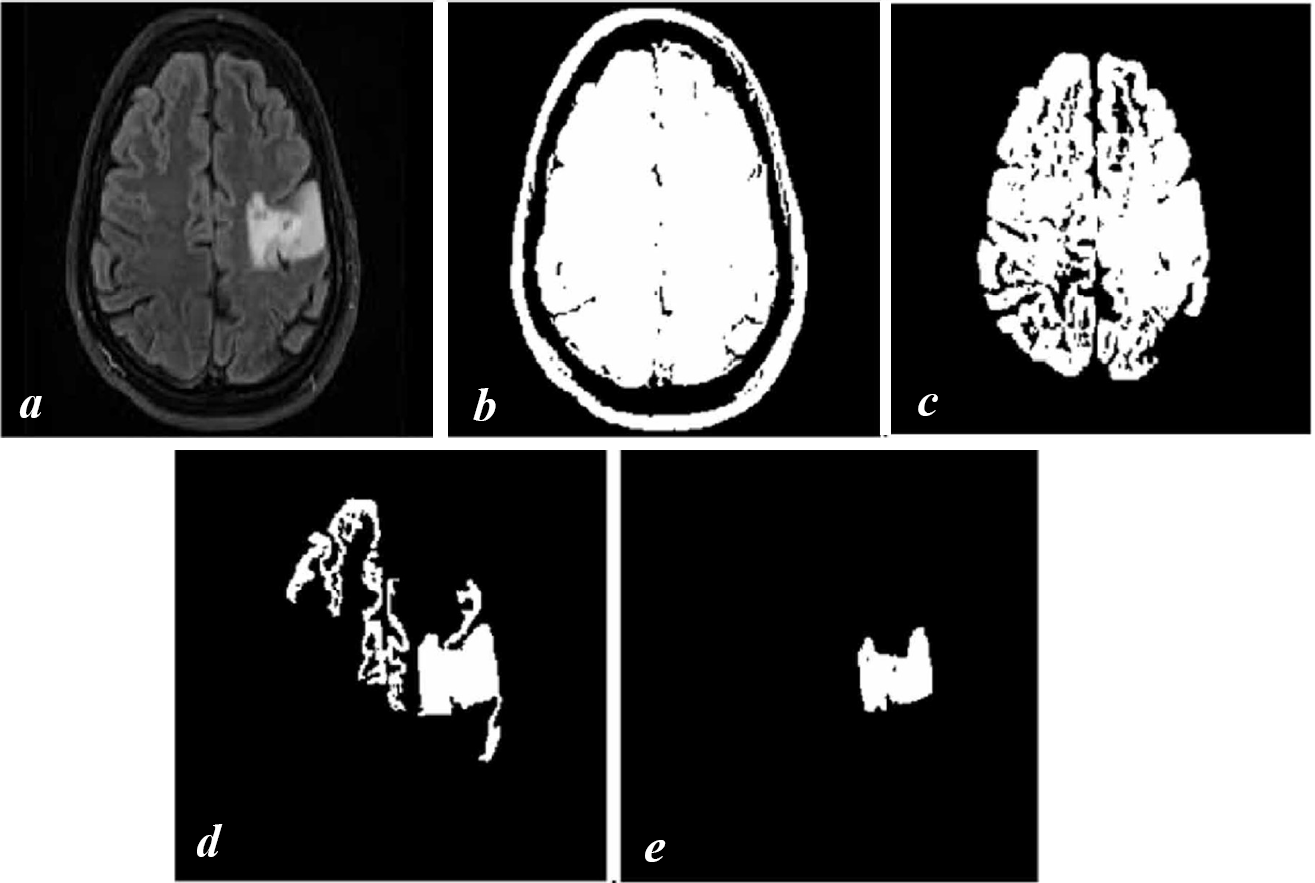
\includegraphics[width=0.8\columnwidth]{figures/Fig28.png}
	\caption{Example of the segmentation for different mean of BCET: a) original image, b) BCET 120, c) BCET 100, d) BCET 80, e) BCET 60}
	\label{fig28}
\end{figure}

\subsection{Adaptive Median Filtering (AMF)}
Image noise can be briefly defined as random variations in some of the pixel values of an image. We know filters are used to reduce the amount of noise present in an image. There are some outlier pixel values in images, due to these outlier cause disturbance (salt \& pepper) or also called as noise in images. Median filtering is excellent at reducing this type of noise. The filtering algorithm will scan the entire image, using a small matrix and recalculate the value of the center pixel by simply taking the median of all the values inside the matrix.

the median filter considers each pixel in the image in
turn and looks at its nearby neighbors to decide whether or not it is representative of its surroundings. Instead of simply replacing the pixel value with the mean of neighboring pixel values, it replaces it with the median of those values. The median is calculated by first sorting all the pixel values from the surrounding neighborhood into numerical order and then replacing the pixel being considered with the middle pixel value. The following example should clear the concept.

\begin{center}
	\[
	\textit{current value} =  
	\begin{bmatrix}
		19 & 12 & 38 \\
		42 & \textcolor{blue}{11} & 9 \\
		27 & 40 & 33
	\end{bmatrix}
	\]
	\textbf{Sort}: 9 , 11 , 12 , 19 , 27 , 33 , 38 , 40 , 42
	
	\textbf{Median}: 27
	\[
	\textit{after apply filter} =  
	\begin{bmatrix}
		19 & 12 & 38 \\
		42 & \textcolor{blue}{27} & 9 \\
		27 & 40 & 33
	\end{bmatrix}
	\]
\end{center}

The Adaptive Median Filter performs spatial processing to determine which
pixels in an image have been affected by impulse noise. The Adaptive Median Filter classifies pixels as noise by comparing each pixel in the image to its surrounding neighbor pixels. The size of the neighborhood is adjustable, as well as the threshold for the comparison. A pixel that is different from most of its neighbors, as well as being not structurally aligned with those pixels to which it is similar, is labeled as impulse noise. These noise pixels are then replaced by the
median pixel value of the pixels in the neighborhood that have passed the noise labeling test. 

The Adaptive Median Filter needs the following parameters:

\begin{itemize}
	\item \textbf{$S_{xy}$}: the support of the filter centered at (x, y)
	\item \textbf{$Z_{min}$}: minimum gray level value in $S_{xy}$
	\item \textbf{$Z_{max}$}: maximum gray level value in $S_{xy}$
	\item \textbf{$Z_{med}$}: median of gray levels in $S_{xy}$
	\item \textbf{$Z_{xy}$}: gray level at coordinates (x, y)
	\item \textbf{$S_{max}$}: maximum allowed size of $S_{xy}$
\end{itemize}

AMF uses the following algorithm (Algorithm \ref{Algo2}):

\begin{algorithm}[t]
	\caption{Adaptive Median Filter}
	\label{Algo2}
	\begin{spacing}{1.5}
		\begin{algorithmic}[1]
			\State \textbf{Level A:}
			\State A1 = $Z_{med}$ - $Z_{min}$
			\State A2 = $Z_{med}$ - $Z_{max}$
			\If{A1 > 0 AND A2 < 0}
			\State go to \textbf{level B}
			\Else
			\State increase the window size
			\If{window size < $S_{max}$}
			\State repeat level A
			\Else 
			\State output $Z_{xy}$
			\EndIf
			\EndIf
			\State \textbf{Level B:}
			\State B1 =  $Z_{xy}$ -  $Z_{min}$
			\State B2 =  $Z_{xy}$ -  $Z_{max}$
			\If{B1 > 0 AND B2 < 0}
			\State output $Z_{xy}$
			\Else
			\State output $Z_{med}$
			\EndIf
		\end{algorithmic}
	\end{spacing}
\end{algorithm}

\vspace{4cm}

\textbf{Level A} determines if the output of the filter $Z_{med}$ is an impulse or not(black or white). If it is not an impulse we go to \textbf{level B}. On the other hand, if it is an impulse, the window size is increased until it reaches the maximum window size or $Z_{med}$ is not an impulse. 

\textbf{level B} determines if the pixel value at (x, y), that is $Z_{xy}$, is an impulse or not. If it is not an impulse, the algorithm output wont change current $Z_{xy}$. But, if it is an impulse the algorithm output will be  $Z_{med}$. 

\subsection{Otsu’s Thresholding}

Converting a grayscale image to monochrome is a common image
processing task. Otsu's method, named after its inventor Nobuyuki Otsu, is one of many binarization algorithms, it uses data-driven approach which can adaptively find the optimal threshold to distinguish two-class data, by going through all possible threshold values (from 0 to 255), it can find the optimal threshold value of input image. This method can be applied in image segmentation and image binarization, in the current project the use was for image binarization.

Threshold is a value between 0 to 255. For example, if we set threshold value T = 128, then the image is separated into two classes, which are Class 1 (pixel value<= 128) and Class 2 (pixel value> 128) We can say that these two classes represent background and foreground of the input image, respectively.

\subsection{Canny Edge Detection}
In the final step of the algorithm, the 2 segmented images resulted from the segmentation process are combined using opencv \textbf{addWeighted} method by providing desired weights, the tumor being weighted more. This combined image is provided as an argument for the canny edge detection, the method highlights the tumor region and results with detected tumor output image.
There are many other methods which can be used for contour extraction such as Roberts, Prewitt, Sobel, and more complex ones like LoG but we used as a reference shown Canny method to be effective for contour extraction.

\subsection{Architecture of the system}
Figure \ref{fig29} illustrates the architecture of the system.

\newpage
\begin{figure}[H]
	%\resizebox{\linewidth}{!}{
	\centering 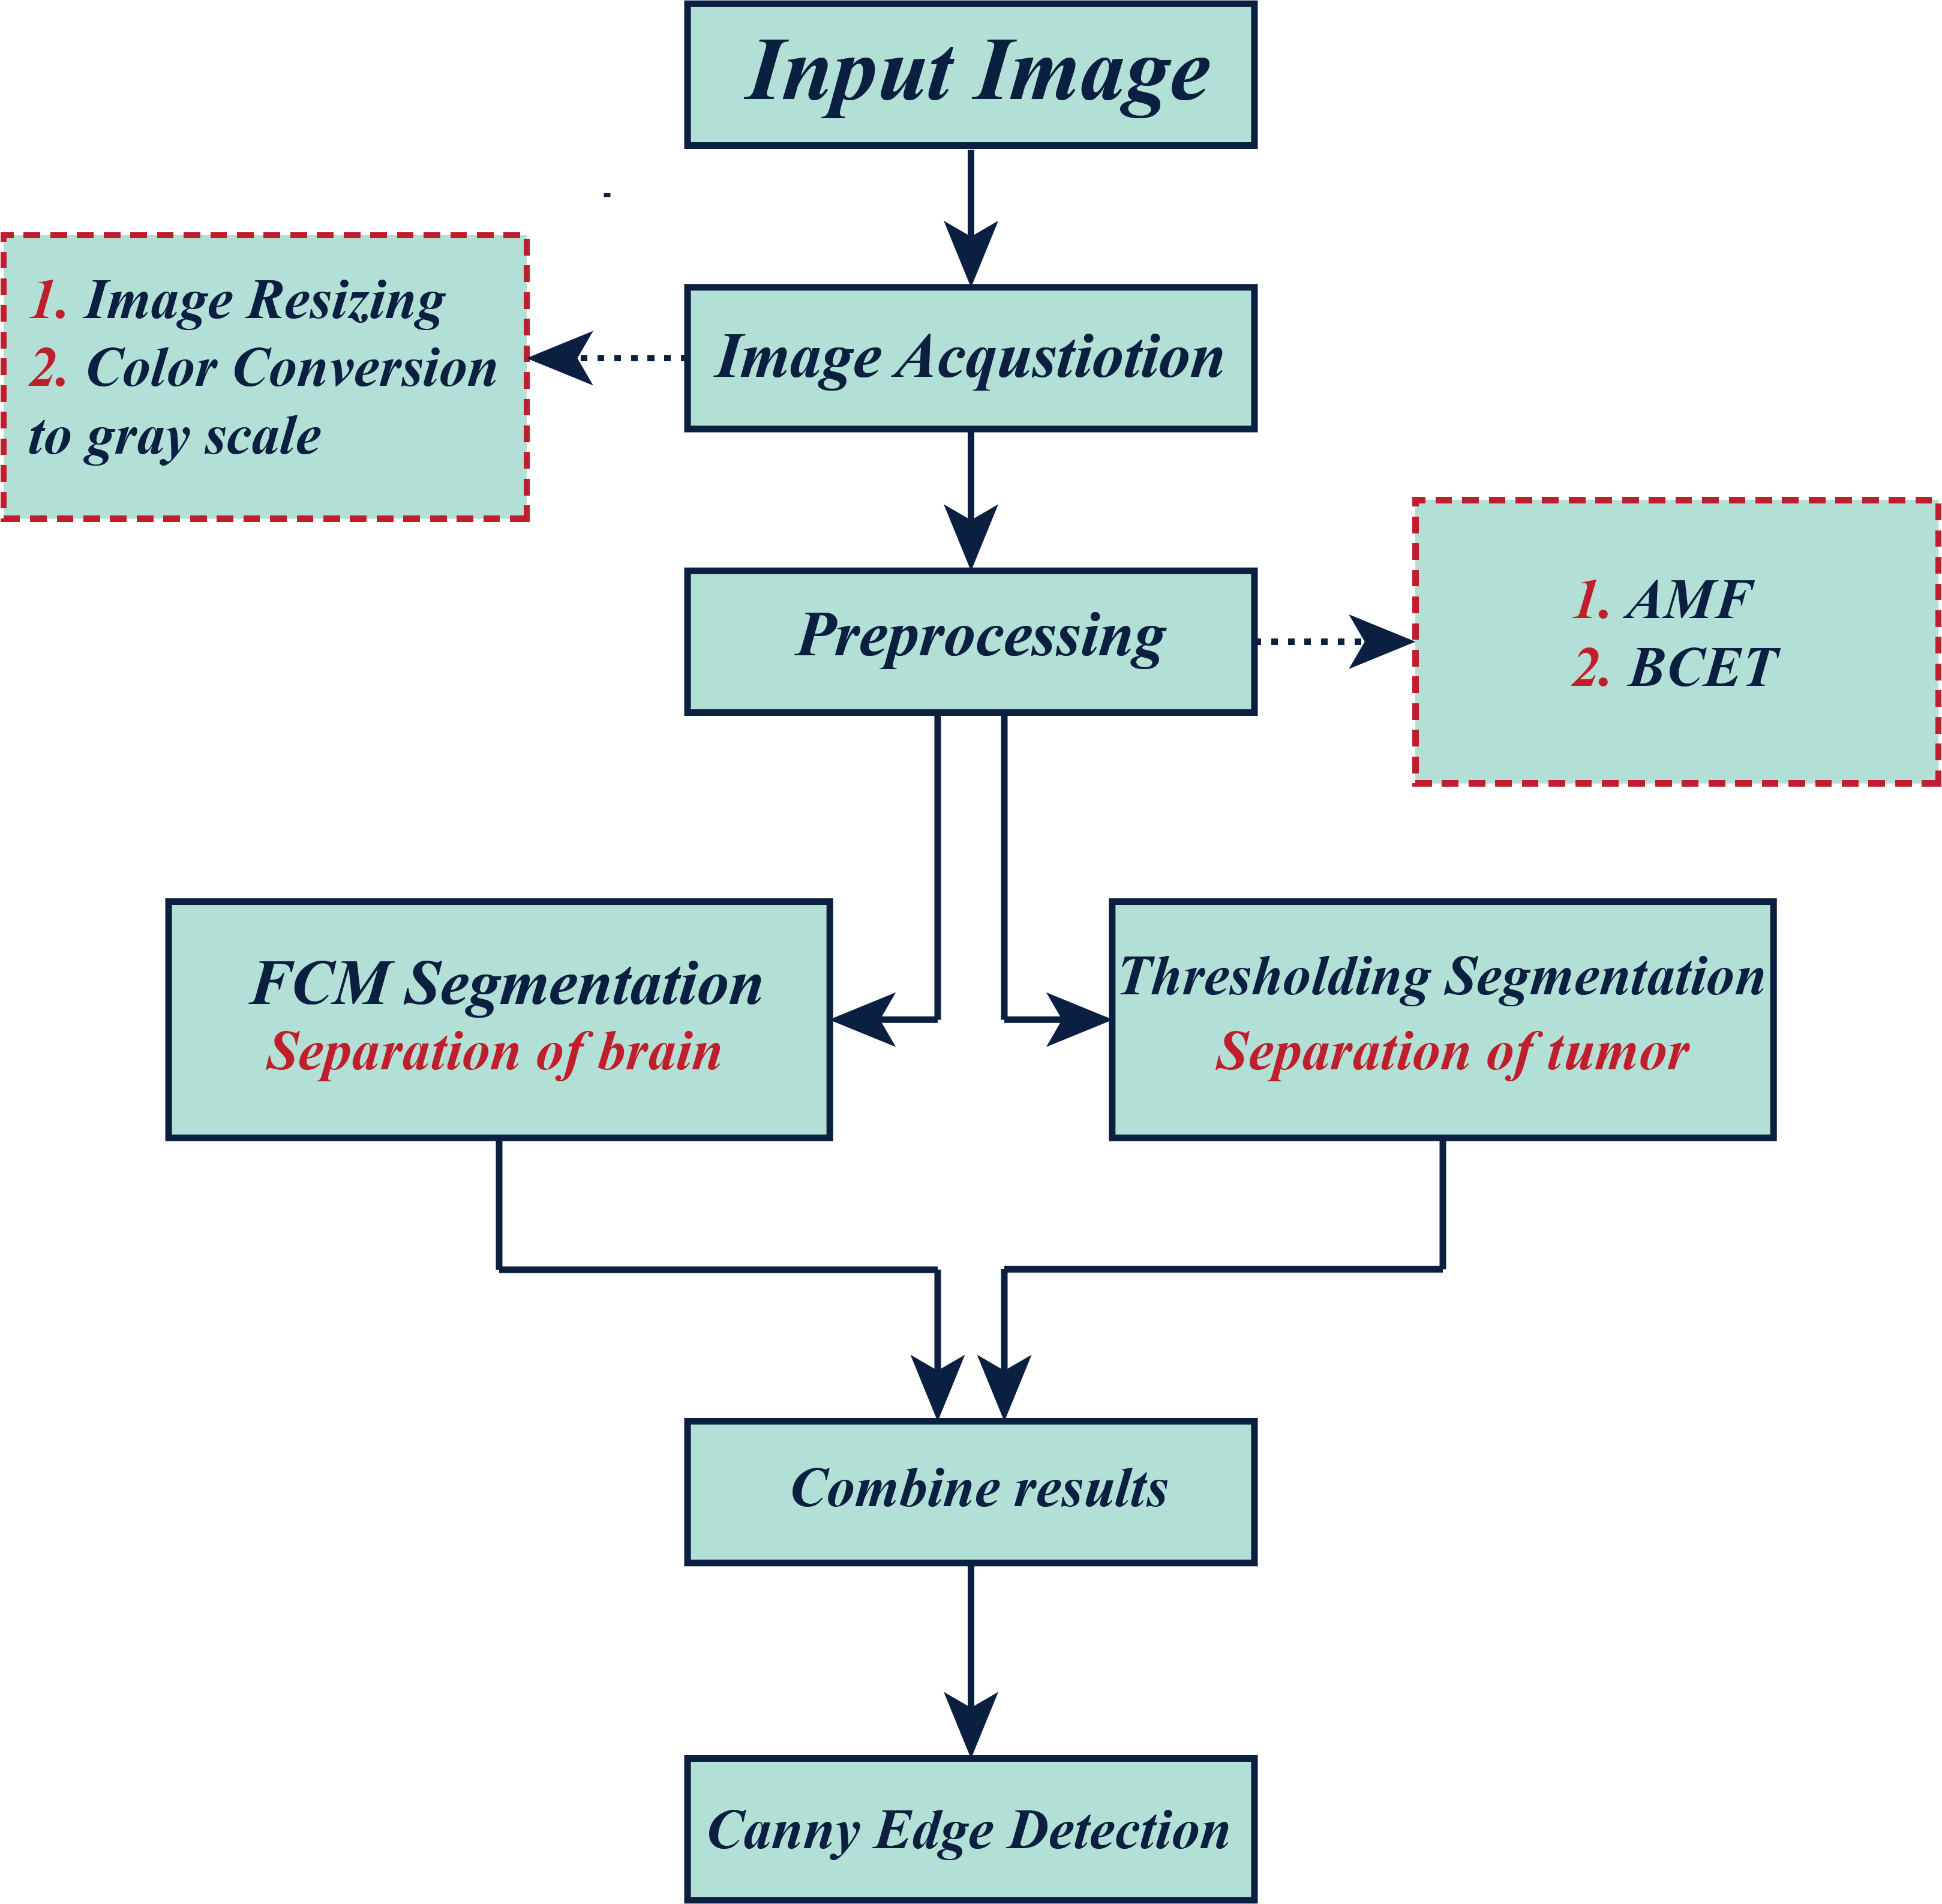
\includegraphics[width=1\columnwidth]{figures/Fig29.png}
	\caption{Architecture of the system}
	\label{fig29}
\end{figure}

\subsection{Implementation}

\begin{tcolorbox}[breakable, size=fbox, boxrule=1pt, pad at break*=1mm,colback=cellbackground, colframe=cellborder]
	\prompt{In}{incolor}{ }{\boxspacing}
	\begin{Verbatim}[commandchars=\\\{\}]
\PY{k+kn}{import} \PY{n+nn}{sys}
\PY{k+kn}{import} \PY{n+nn}{os}
\PY{k+kn}{from} \PY{n+nn}{time} \PY{k+kn}{import} \PY{n}{time}
\PY{k+kn}{import} \PY{n+nn}{cv2}
\PY{k+kn}{import} \PY{n+nn}{numpy} \PY{k}{as} \PY{n+nn}{np}
\PY{k+kn}{import} \PY{n+nn}{matplotlib}\PY{n+nn}{.}\PY{n+nn}{pyplot} \PY{k}{as} \PY{n+nn}{plt}
\PY{k+kn}{import} \PY{n+nn}{skfuzzy} \PY{k}{as} \PY{n+nn}{fuzz}
	\end{Verbatim}
\end{tcolorbox}

\begin{tcolorbox}[breakable, size=fbox, boxrule=1pt, pad at break*=1mm,colback=cellbackground, colframe=cellborder]
	\prompt{In}{incolor}{ }{\boxspacing}
	\begin{Verbatim}[commandchars=\\\{\}]
\PY{k}{def} \PY{n+nf}{AdaptiveMedianFilter}\PY{p}{(}\PY{n}{grayimage}\PY{p}{)}\PY{p}{:}
    \PY{k}{try}\PY{p}{:}
        \PY{n}{img\PYZus{}out} \PY{o}{=} \PY{n}{grayimage}\PY{o}{.}\PY{n}{copy}\PY{p}{(}\PY{p}{)}
        \PY{n}{height} \PY{o}{=} \PY{n}{grayimage}\PY{o}{.}\PY{n}{shape}\PY{p}{[}\PY{l+m+mi}{0}\PY{p}{]}
        \PY{n}{width} \PY{o}{=} \PY{n}{grayimage}\PY{o}{.}\PY{n}{shape}\PY{p}{[}\PY{l+m+mi}{1}\PY{p}{]}
        \PY{k}{for} \PY{n}{i} \PY{o+ow}{in} \PY{n}{np}\PY{o}{.}\PY{n}{arange}\PY{p}{(}\PY{l+m+mi}{6}\PY{p}{,} \PY{n}{height} \PY{o}{\PYZhy{}} \PY{l+m+mi}{5}\PY{p}{)}\PY{p}{:}
            \PY{k}{for} \PY{n}{j} \PY{o+ow}{in} \PY{n}{np}\PY{o}{.}\PY{n}{arange}\PY{p}{(}\PY{l+m+mi}{6}\PY{p}{,} \PY{n}{width} \PY{o}{\PYZhy{}} \PY{l+m+mi}{5}\PY{p}{)}\PY{p}{:}
                \PY{n}{neighbors} \PY{o}{=} \PY{p}{[}\PY{p}{]}
		
                \PY{k}{for} \PY{n}{k} \PY{o+ow}{in} \PY{n}{np}\PY{o}{.}\PY{n}{arange}\PY{p}{(}\PY{o}{\PYZhy{}}\PY{l+m+mi}{6}\PY{p}{,} \PY{l+m+mi}{6}\PY{p}{)}\PY{p}{:}
                    \PY{k}{for} \PY{n}{l} \PY{o+ow}{in} \PY{n}{np}\PY{o}{.}\PY{n}{arange}\PY{p}{(}\PY{o}{\PYZhy{}}\PY{l+m+mi}{6}\PY{p}{,} \PY{l+m+mi}{6}\PY{p}{)}\PY{p}{:}
                        \PY{n}{a} \PY{o}{=} \PY{n}{grayimage}\PY{o}{.}\PY{n}{item}\PY{p}{(}\PY{n}{i} \PY{o}{+} \PY{n}{k}\PY{p}{,} \PY{n}{j} \PY{o}{+} \PY{n}{l}\PY{p}{)}
                        \PY{n}{neighbors}\PY{o}{.}\PY{n}{append}\PY{p}{(}\PY{n}{a}\PY{p}{)}
        \PY{n}{neighbors}\PY{o}{.}\PY{n}{sort}\PY{p}{(}\PY{p}{)}
        \PY{n}{median} \PY{o}{=} \PY{n}{neighbors}\PY{p}{[}\PY{l+m+mi}{30}\PY{p}{]}
        \PY{n}{b} \PY{o}{=} \PY{n}{median}
        \PY{n}{img\PYZus{}out}\PY{o}{.}\PY{n}{itemset}\PY{p}{(}\PY{p}{(}\PY{n}{i}\PY{p}{,} \PY{n}{j}\PY{p}{)}\PY{p}{,} \PY{n}{b}\PY{p}{)}
		
    \PY{k}{except} \PY{n+ne}{Exception} \PY{k}{as} \PY{n}{e}\PY{p}{:}
        \PY{n+nb}{print}\PY{p}{(}\PY{l+s+s2}{\PYZdq{}}\PY{l+s+s2}{Error=}\PY{l+s+s2}{\PYZdq{}} \PY{o}{+} \PY{n}{e}\PY{o}{.}\PY{n}{args}\PY{p}{[}\PY{l+m+mi}{0}\PY{p}{]}\PY{p}{)}
        \PY{n}{tb} \PY{o}{=} \PY{n}{sys}\PY{o}{.}\PY{n}{exc\PYZus{}info}\PY{p}{(}\PY{p}{)}\PY{p}{[}\PY{l+m+mi}{2}\PY{p}{]}
		\PY{n+nb}{print}\PY{p}{(}\PY{n}{tb}\PY{o}{.}\PY{n}{tb\PYZus{}lineno}\PY{p}{)}
		
    \PY{k}{return} \PY{n}{img\PYZus{}out}\PY{o}{.}\PY{n}{astype}\PY{p}{(}\PY{n}{np}\PY{o}{.}\PY{n}{uint8}\PY{p}{)}
	\end{Verbatim}
\end{tcolorbox}

\begin{tcolorbox}[breakable, size=fbox, boxrule=1pt, pad at break*=1mm,colback=cellbackground, colframe=cellborder]
	\prompt{In}{incolor}{ }{\boxspacing}
	\begin{Verbatim}[commandchars=\\\{\}]
\PY{k}{def} \PY{n+nf}{BalanceContrastEnhancementTechnique}\PY{p}{(}\PY{n}{gray\PYZus{}image}\PY{p}{)}\PY{p}{:}
    \PY{n}{x} \PY{o}{=} \PY{n}{im2double}\PY{p}{(}\PY{n}{gray\PYZus{}image}\PY{p}{)} \PY{c+c1}{\PYZsh{} INPUT IMAGE}
    \PY{n}{Lmin} \PY{o}{=} \PY{n}{np}\PY{o}{.}\PY{n}{min}\PY{p}{(}\PY{n}{x}\PY{o}{.}\PY{n}{ravel}\PY{p}{(}\PY{p}{)}\PY{p}{)} \PY{c+c1}{\PYZsh{} MINIMUM OF INPUT IMAGE}
    \PY{n}{Lmax} \PY{o}{=}\PY{n}{np}\PY{o}{.}\PY{n}{max}\PY{p}{(}\PY{n}{x}\PY{o}{.}\PY{n}{ravel}\PY{p}{(}\PY{p}{)}\PY{p}{)} \PY{c+c1}{\PYZsh{} MAXIMUM OF INPUT IMAGE}
    \PY{n}{Lmean} \PY{o}{=} \PY{n}{np}\PY{o}{.}\PY{n}{mean}\PY{p}{(}\PY{n}{x}\PY{p}{)} \PY{c+c1}{\PYZsh{} MEAN OF INPUT IMAGE}
    \PY{n}{LMssum} \PY{o}{=} \PY{n}{np}\PY{o}{.}\PY{n}{mean}\PY{p}{(}\PY{n+nb}{pow}\PY{p}{(}\PY{n}{x}\PY{p}{,}\PY{l+m+mi}{2}\PY{p}{)}\PY{p}{)} \PY{c+c1}{\PYZsh{} MEAN SQUARE SUM OF INPUT IMAGE}

    \PY{n}{Gmin} \PY{o}{=} \PY{l+m+mi}{0} \PY{c+c1}{\PYZsh{} MINIMUM OF OUTPUT IMAGE}
    \PY{n}{Gmax} \PY{o}{=} \PY{l+m+mi}{255} \PY{c+c1}{\PYZsh{} MAXIMUM OF OUTPUT IMAGE}
    \PY{n}{Gmean} \PY{o}{=}\PY{l+m+mi}{85} \PY{c+c1}{\PYZsh{} MEAN OF OUTPUT IMAGE 80 (Recomended)}

    \PY{n}{bnum} \PY{o}{=} \PY{n+nb}{pow}\PY{p}{(}\PY{n}{Lmax}\PY{p}{,}\PY{l+m+mi}{2}\PY{p}{)} \PY{o}{*} \PY{p}{(}\PY{n}{Gmean} \PY{o}{\PYZhy{}} \PY{n}{Gmin}\PY{p}{)} \PY{o}{\PYZhy{}} \PY{n}{LMssum} \PY{o}{*} \PY{p}{(}\PY{n}{Gmax} \PY{o}{\PYZhy{}} \PY{n}{Gmin}\PY{p}{)} \PY{o}{+}
    \PY{n+nb}{pow}\PY{p}{(}\PY{n}{Lmin}\PY{p}{,}\PY{l+m+mi}{2}\PY{p}{)} \PY{o}{*} \PY{p}{(}\PY{n}{Gmax} \PY{o}{\PYZhy{}} \PY{n}{Gmean}\PY{p}{)}
    \PY{n}{bden} \PY{o}{=} \PY{l+m+mi}{2} \PY{o}{*} \PY{p}{(}\PY{n}{Lmax} \PY{o}{*} \PY{p}{(}\PY{n}{Gmean} \PY{o}{\PYZhy{}} \PY{n}{Gmin}\PY{p}{)} \PY{o}{\PYZhy{}} \PY{n}{Lmean} \PY{o}{*} \PY{p}{(}\PY{n}{Gmax} \PY{o}{\PYZhy{}} \PY{n}{Gmin}\PY{p}{)} \PY{o}{+} \PY{n}{Lmin} \PY{o}{*}
    \PY{p}{(}\PY{n}{Gmax} \PY{o}{\PYZhy{}} \PY{n}{Gmean}\PY{p}{)}\PY{p}{)}

    \PY{n}{b} \PY{o}{=} \PY{n}{bnum} \PY{o}{/} \PY{n}{bden}
    \PY{n}{a} \PY{o}{=} \PY{p}{(}\PY{n}{Gmax} \PY{o}{\PYZhy{}} \PY{n}{Gmin}\PY{p}{)} \PY{o}{/} \PY{p}{(}\PY{p}{(}\PY{n}{Lmax} \PY{o}{\PYZhy{}} \PY{n}{Lmin}\PY{p}{)} \PY{o}{*} \PY{p}{(}\PY{n}{Lmax} \PY{o}{+} \PY{n}{Lmin} \PY{o}{\PYZhy{}} \PY{l+m+mi}{2} \PY{o}{*} \PY{n}{b}\PY{p}{)}\PY{p}{)}
    \PY{n}{c} \PY{o}{=} \PY{n}{Gmin} \PY{o}{\PYZhy{}} \PY{n}{a} \PY{o}{*} \PY{n+nb}{pow}\PY{p}{(}\PY{p}{(}\PY{n}{Lmin} \PY{o}{\PYZhy{}} \PY{n}{b}\PY{p}{)}\PY{p}{,} \PY{l+m+mi}{2}\PY{p}{)}
    \PY{n}{y} \PY{o}{=} \PY{n}{a} \PY{o}{*}\PY{n+nb}{pow}\PY{p}{(}\PY{p}{(}\PY{n}{x} \PY{o}{\PYZhy{}} \PY{n}{b}\PY{p}{)}\PY{p}{,}\PY{l+m+mi}{2}\PY{p}{)}\PY{o}{+} \PY{n}{c} \PY{c+c1}{\PYZsh{} PARABOLIC FUNCTION}
    \PY{n}{y} \PY{o}{=} \PY{n}{y}\PY{o}{.}\PY{n}{astype}\PY{p}{(}\PY{n}{np}\PY{o}{.}\PY{n}{uint8}\PY{p}{)}

    \PY{k}{return} \PY{n}{y}
	\end{Verbatim}
\end{tcolorbox}

\begin{tcolorbox}[breakable, size=fbox, boxrule=1pt, pad at break*=1mm,colback=cellbackground, colframe=cellborder]
	\prompt{In}{incolor}{ }{\boxspacing}
	\begin{Verbatim}[commandchars=\\\{\}]
\PY{k}{def} \PY{n+nf}{im2double}\PY{p}{(}\PY{n}{im}\PY{p}{)}\PY{p}{:}
    \PY{n}{min\PYZus{}val} \PY{o}{=} \PY{n}{np}\PY{o}{.}\PY{n}{min}\PY{p}{(}\PY{n}{im}\PY{o}{.}\PY{n}{ravel}\PY{p}{(}\PY{p}{)}\PY{p}{)}
    \PY{n}{max\PYZus{}val} \PY{o}{=} \PY{n}{np}\PY{o}{.}\PY{n}{max}\PY{p}{(}\PY{n}{im}\PY{o}{.}\PY{n}{ravel}\PY{p}{(}\PY{p}{)}\PY{p}{)}
    \PY{n}{out} \PY{o}{=} \PY{p}{(}\PY{n}{im}\PY{o}{.}\PY{n}{astype}\PY{p}{(}\PY{l+s+s1}{\PYZsq{}}\PY{l+s+s1}{float}\PY{l+s+s1}{\PYZsq{}}\PY{p}{)} \PY{o}{\PYZhy{}} \PY{n}{min\PYZus{}val}\PY{p}{)} \PY{o}{/} \PY{p}{(}\PY{n}{max\PYZus{}val} \PY{o}{\PYZhy{}} \PY{n}{min\PYZus{}val}\PY{p}{)}
    \PY{k}{return} \PY{n}{out}
	\end{Verbatim}
\end{tcolorbox}

NumPy python package is used to calculate the min,max,mean of the input
image by converting the given image pixel array to double precession and
flattening out the array using NumPy ravel function and applying desired
min,max functions existing in NumPy package. The resultant `y' is the
new enhanced/stretched contrast image, this image is used in further
processing for thresholding and contour extraction.

\begin{tcolorbox}[breakable, size=fbox, boxrule=1pt, pad at break*=1mm,colback=cellbackground, colframe=cellborder]
	\prompt{In}{incolor}{ }{\boxspacing}
	\begin{Verbatim}[commandchars=\\\{\}]
\PY{k}{def} \PY{n+nf}{FCM}\PY{p}{(}\PY{n}{image\PYZus{}bcet}\PY{p}{)}\PY{p}{:}
    \PY{n}{list\PYZus{}img} \PY{o}{=} \PY{p}{[}\PY{p}{]}
    \PY{n}{img} \PY{o}{=}\PY{n}{cv2}\PY{o}{.}\PY{n}{imread}\PY{p}{(}\PY{l+s+s2}{\PYZdq{}}\PY{l+s+s2}{C:/Users/Poorya/Desktop/}\PY{l+s+s2}{\PYZdq{}}\PY{o}{+}\PY{n+nb}{str}\PY{p}{(}\PY{n}{image\PYZus{}bcet}\PY{p}{)}\PY{p}{)}

    \PY{n}{rgb\PYZus{}img} \PY{o}{=} \PY{n}{img}\PY{o}{.}\PY{n}{reshape}\PY{p}{(}\PY{p}{(}\PY{n}{img}\PY{o}{.}\PY{n}{shape}\PY{p}{[}\PY{l+m+mi}{0}\PY{p}{]} \PY{o}{*} \PY{n}{img}\PY{o}{.}\PY{n}{shape}\PY{p}{[}\PY{l+m+mi}{1}\PY{p}{]}\PY{p}{,} \PY{l+m+mi}{3}\PY{p}{)}\PY{p}{)}
    \PY{n}{list\PYZus{}img}\PY{o}{.}\PY{n}{append}\PY{p}{(}\PY{n}{rgb\PYZus{}img}\PY{p}{)}
    \PY{n}{n\PYZus{}data} \PY{o}{=} \PY{n+nb}{len}\PY{p}{(}\PY{n}{list\PYZus{}img}\PY{p}{)}
    \PY{n}{clusters} \PY{o}{=} \PY{p}{[}\PY{l+m+mi}{2}\PY{p}{]}

    \PY{k}{for} \PY{n}{index}\PY{p}{,} \PY{n}{rgb\PYZus{}img} \PY{o+ow}{in} \PY{n+nb}{enumerate}\PY{p}{(}\PY{n}{list\PYZus{}img}\PY{p}{)}\PY{p}{:}
        \PY{n}{img} \PY{o}{=} \PY{n}{np}\PY{o}{.}\PY{n}{reshape}\PY{p}{(}\PY{n}{rgb\PYZus{}img}\PY{p}{,} \PY{p}{(}\PY{l+m+mi}{256}\PY{p}{,} \PY{l+m+mi}{256}\PY{p}{,} \PY{l+m+mi}{3}\PY{p}{)}\PY{p}{)}\PY{o}{.}\PY{n}{astype}\PY{p}{(}\PY{n}{np}\PY{o}{.}\PY{n}{uint8}\PY{p}{)}
        \PY{n}{shape} \PY{o}{=} \PY{n}{np}\PY{o}{.}\PY{n}{shape}\PY{p}{(}\PY{n}{img}\PY{p}{)}
        \PY{c+c1}{\PYZsh{} looping every cluster}
        \PY{k}{for} \PY{n}{i}\PY{p}{,} \PY{n}{cluster} \PY{o+ow}{in} \PY{n+nb}{enumerate}\PY{p}{(}\PY{n}{clusters}\PY{p}{)}\PY{p}{:}
            \PY{c+c1}{\PYZsh{} Fuzzy C Means}
            \PY{n}{new\PYZus{}time} \PY{o}{=} \PY{n}{time}\PY{p}{(}\PY{p}{)}

            \PY{n}{cntr}\PY{p}{,} \PY{n}{u}\PY{p}{,} \PY{n}{u0}\PY{p}{,} \PY{n}{d}\PY{p}{,} \PY{n}{jm}\PY{p}{,} \PY{n}{p}\PY{p}{,} \PY{n}{fpc} \PY{o}{=} \PY{n}{fuzz}\PY{o}{.}\PY{n}{cluster}\PY{o}{.}\PY{n}{cmeans}\PY{p}{(}\PY{n}{rgb\PYZus{}img}\PY{o}{.}\PY{n}{T}\PY{p}{,}
            \PY{n}{cluster}\PY{p}{,} \PY{l+m+mi}{2}\PY{p}{,} \PY{n}{error}\PY{o}{=}\PY{l+m+mf}{0.005}\PY{p}{,} \PY{n}{maxiter}\PY{o}{=}\PY{l+m+mi}{1000}\PY{p}{,} \PY{n}{init}\PY{o}{=}\PY{k+kc}{None}\PY{p}{,} \PY{n}{seed}\PY{o}{=}\PY{l+m+mi}{42}\PY{p}{)}
            \PY{n}{new\PYZus{}img} \PY{o}{=} \PY{n}{change\PYZus{}color\PYZus{}fuzzycmeans}\PY{p}{(}\PY{n}{u}\PY{p}{,} \PY{n}{cntr}\PY{p}{)}
            \PY{n}{fuzzy\PYZus{}img} \PY{o}{=} \PY{n}{np}\PY{o}{.}\PY{n}{reshape}\PY{p}{(}\PY{n}{new\PYZus{}img}\PY{p}{,} \PY{n}{shape}\PY{p}{)}\PY{o}{.}\PY{n}{astype}\PY{p}{(}\PY{n}{np}\PY{o}{.}\PY{n}{uint8}\PY{p}{)}
            \PY{n}{ret}\PY{p}{,} \PY{n}{seg\PYZus{}img} \PY{o}{=} \PY{n}{cv2}\PY{o}{.}\PY{n}{threshold}\PY{p}{(}\PY{n}{fuzzy\PYZus{}img}\PY{p}{,}\PY{n}{np}\PY{o}{.}\PY{n}{max}\PY{p}{(}\PY{n}{fuzzy\PYZus{}img}\PY{p}{)} \PY{o}{\PYZhy{}}
            \PY{l+m+mi}{1}\PY{p}{,}\PY{l+m+mi}{255}\PY{p}{,}\PY{n}{cv2}\PY{o}{.}\PY{n}{THRESH\PYZus{}BINARY}\PY{p}{)}

            \PY{n}{seg\PYZus{}img\PYZus{}1d} \PY{o}{=} \PY{n}{seg\PYZus{}img}\PY{p}{[}\PY{p}{:}\PY{p}{,} \PY{p}{:}\PY{p}{,} \PY{l+m+mi}{1}\PY{p}{]}
            \PY{n}{bwfim1} \PY{o}{=} \PY{n}{bwareaopen}\PY{p}{(}\PY{n}{seg\PYZus{}img\PYZus{}1d}\PY{p}{,} \PY{l+m+mi}{500}\PY{p}{)}
            \PY{n}{bwfim2} \PY{o}{=} \PY{n}{imclearborder}\PY{p}{(}\PY{n}{bwfim1}\PY{p}{)}

            \PY{n}{cv2}\PY{o}{.}\PY{n}{imwrite}\PY{p}{(}\PY{l+s+s1}{\PYZsq{}}\PY{l+s+s1}{C:/Users/Poorya/Desktop/border.jpg}\PY{l+s+s1}{\PYZsq{}}\PY{p}{,} \PY{n}{bwfim2}\PY{p}{)}


            \PY{n}{bwfim3} \PY{o}{=} \PY{n}{imfill}\PY{p}{(}\PY{n}{bwfim2}\PY{p}{)}    

            \PY{n}{cv2}\PY{o}{.}\PY{n}{imwrite}\PY{p}{(}\PY{l+s+s1}{\PYZsq{}}\PY{l+s+s1}{C:/Users/Poorya/Desktop/FCM.jpg}\PY{l+s+s1}{\PYZsq{}}\PY{p}{,} \PY{n}{bwfim3}\PY{p}{)}
    \PY{k}{return} \PY{n}{bwfim3}
	\end{Verbatim}
\end{tcolorbox}

\begin{tcolorbox}[breakable, size=fbox, boxrule=1pt, pad at break*=1mm,colback=cellbackground, colframe=cellborder]
	\prompt{In}{incolor}{ }{\boxspacing}
	\begin{Verbatim}[commandchars=\\\{\}]
\PY{k}{def} \PY{n+nf}{change\PYZus{}color\PYZus{}fuzzycmeans}\PY{p}{(}\PY{n}{cluster\PYZus{}membership}\PY{p}{,} \PY{n}{clusters}\PY{p}{)}\PY{p}{:}
    \PY{n}{img} \PY{o}{=} \PY{p}{[}\PY{p}{]}
    \PY{k}{for} \PY{n}{pix} \PY{o+ow}{in} \PY{n}{cluster\PYZus{}membership}\PY{o}{.}\PY{n}{T}\PY{p}{:}
        \PY{n}{img}\PY{o}{.}\PY{n}{append}\PY{p}{(}\PY{n}{clusters}\PY{p}{[}\PY{n}{np}\PY{o}{.}\PY{n}{argmax}\PY{p}{(}\PY{n}{pix}\PY{p}{)}\PY{p}{]}\PY{p}{)}
    \PY{k}{return} \PY{n}{img}
	\end{Verbatim}
\end{tcolorbox}

\begin{tcolorbox}[breakable, size=fbox, boxrule=1pt, pad at break*=1mm,colback=cellbackground, colframe=cellborder]
	\prompt{In}{incolor}{ }{\boxspacing}
	\begin{Verbatim}[commandchars=\\\{\}]
\PY{k}{def} \PY{n+nf}{imfill}\PY{p}{(}\PY{n}{im\PYZus{}th}\PY{p}{)}\PY{p}{:}
    \PY{n}{im\PYZus{}floodfill} \PY{o}{=} \PY{n}{im\PYZus{}th}\PY{o}{.}\PY{n}{copy}\PY{p}{(}\PY{p}{)}
    \PY{c+c1}{\PYZsh{} Mask used to flood filling.}
    \PY{c+c1}{\PYZsh{} Notice the size needs to be 2 pixels than the image.}
    \PY{n}{h}\PY{p}{,} \PY{n}{w} \PY{o}{=} \PY{n}{im\PYZus{}th}\PY{o}{.}\PY{n}{shape}\PY{p}{[}\PY{p}{:}\PY{l+m+mi}{2}\PY{p}{]}
    \PY{n}{mask} \PY{o}{=} \PY{n}{np}\PY{o}{.}\PY{n}{zeros}\PY{p}{(}\PY{p}{(}\PY{n}{h} \PY{o}{+} \PY{l+m+mi}{2}\PY{p}{,} \PY{n}{w} \PY{o}{+} \PY{l+m+mi}{2}\PY{p}{)}\PY{p}{,} \PY{n}{np}\PY{o}{.}\PY{n}{uint8}\PY{p}{)}
    \PY{c+c1}{\PYZsh{} Floodfill from point (0, 0)}
    \PY{n}{cv2}\PY{o}{.}\PY{n}{floodFill}\PY{p}{(}\PY{n}{im\PYZus{}floodfill}\PY{p}{,} \PY{n}{mask}\PY{p}{,} \PY{p}{(}\PY{l+m+mi}{0}\PY{p}{,} \PY{l+m+mi}{0}\PY{p}{)}\PY{p}{,} \PY{l+m+mi}{255}\PY{p}{)}\PY{p}{;}
    \PY{c+c1}{\PYZsh{} Invert floodfilled image}
    \PY{n}{im\PYZus{}floodfill\PYZus{}inv} \PY{o}{=} \PY{n}{cv2}\PY{o}{.}\PY{n}{bitwise\PYZus{}not}\PY{p}{(}\PY{n}{im\PYZus{}floodfill}\PY{p}{)}
    \PY{c+c1}{\PYZsh{} Combine the two images to get the foreground.}
    \PY{n}{im\PYZus{}out} \PY{o}{=} \PY{n}{im\PYZus{}th} \PY{o}{|} \PY{n}{im\PYZus{}floodfill\PYZus{}inv}
    \PY{k}{return} \PY{n}{im\PYZus{}out}
	\end{Verbatim}
\end{tcolorbox}

 After clustering, the cluster centers are passed to custom function and
a new image is constructed according to the cluster membership.
Thresholding is performed on this image using opencv threshold method,
this is usually done for optimal contour extraction.

{Contours} can be explained simply as a curve joining all the continuous
points (along the boundary), having same color or intensity. The
contours are a useful tool for shape analysis and object detection and
recognition.Here they suggest performing thresholding before contour
extraction. The contour extraction is applied at 2 different stages:

\begin{tcolorbox}[breakable, size=fbox, boxrule=1pt, pad at break*=1mm,colback=cellbackground, colframe=cellborder]
	\prompt{In}{incolor}{ }{\boxspacing}
	\begin{Verbatim}[commandchars=\\\{\}]
\PY{k}{def} \PY{n+nf}{bwareaopen}\PY{p}{(}\PY{n}{imgBW}\PY{p}{,} \PY{n}{areaPixels}\PY{p}{)}\PY{p}{:}
    \PY{c+c1}{\PYZsh{} Given a black and white image, first find all of its contours}
    \PY{n}{imgBWcopy} \PY{o}{=} \PY{n}{imgBW}\PY{o}{.}\PY{n}{copy}\PY{p}{(}\PY{p}{)}
    \PY{n}{contours}\PY{p}{,} \PY{n}{hierarchy} \PY{o}{=} \PY{n}{cv2}\PY{o}{.}\PY{n}{findContours}\PY{p}{(}\PY{n}{imgBWcopy}\PY{o}{.}\PY{n}{copy}\PY{p}{(}\PY{p}{)}\PY{p}{,} \PY{n}{cv2}\PY{o}{.}\PY{n}{RETR\PYZus{}LIST}\PY{p}{,}\PY{n}{cv2}\PY{o}{.}\PY{n}{CHAIN\PYZus{}APPROX\PYZus{}SIMPLE}\PY{p}{)}
    \PY{c+c1}{\PYZsh{} For each contour, determine its total occupying area}
    \PY{k}{for} \PY{n}{idx} \PY{o+ow}{in} \PY{n}{np}\PY{o}{.}\PY{n}{arange}\PY{p}{(}\PY{n+nb}{len}\PY{p}{(}\PY{n}{contours}\PY{p}{)}\PY{p}{)}\PY{p}{:}
        \PY{n}{area} \PY{o}{=} \PY{n}{cv2}\PY{o}{.}\PY{n}{contourArea}\PY{p}{(}\PY{n}{contours}\PY{p}{[}\PY{n}{idx}\PY{p}{]}\PY{p}{)}
        \PY{k}{if} \PY{p}{(}\PY{n}{area} \PY{o}{\PYZgt{}}\PY{o}{=} \PY{l+m+mi}{0} \PY{o+ow}{and} \PY{n}{area} \PY{o}{\PYZlt{}}\PY{o}{=} \PY{n}{areaPixels}\PY{p}{)}\PY{p}{:}
            \PY{n}{cv2}\PY{o}{.}\PY{n}{drawContours}\PY{p}{(}\PY{n}{imgBWcopy}\PY{p}{,} \PY{n}{contours}\PY{p}{,} \PY{n}{idx}\PY{p}{,} \PY{p}{(}\PY{l+m+mi}{0}\PY{p}{,} \PY{l+m+mi}{0}\PY{p}{,} \PY{l+m+mi}{0}\PY{p}{)}\PY{p}{,} \PY{o}{\PYZhy{}}\PY{l+m+mi}{1}\PY{p}{)}

    \PY{k}{return} \PY{n}{imgBWcopy}
	\end{Verbatim}
\end{tcolorbox}

 The above function determines the total occupying area of each contour
and on comparing with the fixed value of area pixels- set to 500, this
is value is used to preserve and draw the contours which ranges in the
specific area. All the extracted contours which fall in the range are
redrawn using opencv drawcontours method.

The next step is a selection the boundary pixels (edge pixels). A pixel
is considered as boundary pixel if the magnitude of the gradient of this
pixel is greater than that of two neighbors in the direction of the
gradient In the below method, each contour row and column pixel is
evaluated, the row and column check conditions are used to determine the
border of the brain and hence appending to a new list of contours, this
list is redrawn using drawContours method. This image is the final FCM
segmented image.

\begin{tcolorbox}[breakable, size=fbox, boxrule=1pt, pad at break*=1mm,colback=cellbackground, colframe=cellborder]
	\prompt{In}{incolor}{ }{\boxspacing}
	\begin{Verbatim}[commandchars=\\\{\}]
\PY{k}{def} \PY{n+nf}{imclearborder}\PY{p}{(}\PY{n}{imgBW}\PY{p}{)}\PY{p}{:}
    \PY{c+c1}{\PYZsh{} Given a black and white image, first find all of its contours}
    \PY{n}{radius} \PY{o}{=} \PY{l+m+mi}{2}
    \PY{n}{imgBWcopy} \PY{o}{=} \PY{n}{imgBW}\PY{o}{.}\PY{n}{copy}\PY{p}{(}\PY{p}{)}

    \PY{n}{contours}\PY{p}{,} \PY{n}{hierarchy} \PY{o}{=} \PY{n}{cv2}\PY{o}{.}\PY{n}{findContours}\PY{p}{(}\PY{n}{imgBWcopy}\PY{o}{.}\PY{n}{copy}\PY{p}{(}\PY{p}{)}\PY{p}{,} \PY{n}{cv2}\PY{o}{.}\PY{n}{RETR\PYZus{}LIST}\PY{p}{,}\PY{n}{cv2}\PY{o}{.}\PY{n}{CHAIN\PYZus{}APPROX\PYZus{}SIMPLE}\PY{p}{)}

    \PY{c+c1}{\PYZsh{} Get dimensions of image}
    \PY{n}{imgRows} \PY{o}{=} \PY{n}{imgBW}\PY{o}{.}\PY{n}{shape}\PY{p}{[}\PY{l+m+mi}{0}\PY{p}{]}
    \PY{n}{imgCols} \PY{o}{=} \PY{n}{imgBW}\PY{o}{.}\PY{n}{shape}\PY{p}{[}\PY{l+m+mi}{1}\PY{p}{]}
    \PY{n}{contourList} \PY{o}{=} \PY{p}{[}\PY{p}{]} \PY{c+c1}{\PYZsh{} ID list of contours that touch the border}

    \PY{c+c1}{\PYZsh{} For each contour...}
    \PY{k}{for} \PY{n}{idx} \PY{o+ow}{in} \PY{n}{np}\PY{o}{.}\PY{n}{arange}\PY{p}{(}\PY{n+nb}{len}\PY{p}{(}\PY{n}{contours}\PY{p}{)}\PY{p}{)}\PY{p}{:}
        \PY{c+c1}{\PYZsh{} Get the i\PYZsq{}th contour}
        \PY{n}{cnt} \PY{o}{=} \PY{n}{contours}\PY{p}{[}\PY{n}{idx}\PY{p}{]}
        \PY{c+c1}{\PYZsh{} Look at each point in the contour}
        \PY{k}{for} \PY{n}{pt} \PY{o+ow}{in} \PY{n}{cnt}\PY{p}{:}
            \PY{n}{rowCnt} \PY{o}{=} \PY{n}{pt}\PY{p}{[}\PY{l+m+mi}{0}\PY{p}{]}\PY{p}{[}\PY{l+m+mi}{1}\PY{p}{]}
            \PY{n}{colCnt} \PY{o}{=} \PY{n}{pt}\PY{p}{[}\PY{l+m+mi}{0}\PY{p}{]}\PY{p}{[}\PY{l+m+mi}{0}\PY{p}{]}
            \PY{c+c1}{\PYZsh{} If this is within the radius of the border}
            \PY{c+c1}{\PYZsh{} this contour goes bye bye!}
            \PY{n}{check1} \PY{o}{=} \PY{p}{(}\PY{n}{rowCnt} \PY{o}{\PYZgt{}}\PY{o}{=} \PY{l+m+mi}{0} \PY{o+ow}{and} \PY{n}{rowCnt} \PY{o}{\PYZlt{}} \PY{n}{radius}\PY{p}{)} \PY{o+ow}{or} \PY{p}{(}\PY{n}{rowCnt}
            \PY{o}{\PYZgt{}}\PY{o}{=} \PY{n}{imgRows} \PY{o}{\PYZhy{}} \PY{l+m+mi}{1} \PY{o}{\PYZhy{}} \PY{n}{radius} \PY{o+ow}{and} \PY{n}{rowCnt} \PY{o}{\PYZlt{}} \PY{n}{imgRows}\PY{p}{)}
            \PY{n}{check2} \PY{o}{=} \PY{p}{(}\PY{n}{colCnt} \PY{o}{\PYZgt{}}\PY{o}{=} \PY{l+m+mi}{0} \PY{o+ow}{and} \PY{n}{colCnt} \PY{o}{\PYZlt{}} \PY{n}{radius}\PY{p}{)} \PY{o+ow}{or} \PY{p}{(}\PY{n}{colCnt} \PY{o}{\PYZgt{}}\PY{o}{=}
            \PY{n}{imgCols} \PY{o}{\PYZhy{}} \PY{l+m+mi}{1} \PY{o}{\PYZhy{}} \PY{n}{radius} \PY{o+ow}{and} \PY{n}{colCnt} \PY{o}{\PYZlt{}} \PY{n}{imgCols}\PY{p}{)} 

            \PY{k}{if} \PY{n}{check1} \PY{o+ow}{or} \PY{n}{check2}\PY{p}{:}
                \PY{n}{contourList}\PY{o}{.}\PY{n}{append}\PY{p}{(}\PY{n}{idx}\PY{p}{)}
                \PY{k}{break}

        \PY{k}{for} \PY{n}{idx} \PY{o+ow}{in} \PY{n}{contourList}\PY{p}{:}
            \PY{n}{cv2}\PY{o}{.}\PY{n}{drawContours}\PY{p}{(}\PY{n}{imgBWcopy}\PY{p}{,} \PY{n}{contours}\PY{p}{,} \PY{n}{idx}\PY{p}{,} \PY{p}{(}\PY{l+m+mi}{0}\PY{p}{,} \PY{l+m+mi}{0}\PY{p}{,} \PY{l+m+mi}{0}\PY{p}{)}\PY{p}{,} \PY{o}{\PYZhy{}}\PY{l+m+mi}{1}\PY{p}{)}           
    \PY{k}{return} \PY{n}{imgBWcopy}
	\end{Verbatim}
\end{tcolorbox}

\begin{tcolorbox}[breakable, size=fbox, boxrule=1pt, pad at break*=1mm,colback=cellbackground, colframe=cellborder]
	\prompt{In}{incolor}{ }{\boxspacing}
	\begin{Verbatim}[commandchars=\\\{\}]
\PY{k}{def} \PY{n+nf}{Thresholding}\PY{p}{(}\PY{n}{image\PYZus{}bcet}\PY{p}{)}\PY{p}{:}
    \PY{n}{blur} \PY{o}{=} \PY{n}{cv2}\PY{o}{.}\PY{n}{GaussianBlur}\PY{p}{(}\PY{n}{image\PYZus{}bcet}\PY{p}{,}\PY{p}{(}\PY{l+m+mi}{5}\PY{p}{,}\PY{l+m+mi}{5}\PY{p}{)}\PY{p}{,}\PY{l+m+mi}{0}\PY{p}{)}
    \PY{n}{T}\PY{p}{,} \PY{n}{thresh\PYZus{}f} \PY{o}{=} \PY{n}{cv2}\PY{o}{.}\PY{n}{threshold}\PY{p}{(}\PY{n}{blur}\PY{p}{,}\PY{l+m+mi}{200}\PY{p}{,}\PY{l+m+mi}{255}\PY{p}{,}   \PY{n}{cv2}\PY{o}{.}\PY{n}{THRESH\PYZus{}BINARY}\PY{p}{)}
    \PY{k}{return} \PY{n}{thresh\PYZus{}f}
	\end{Verbatim}
\end{tcolorbox}

\begin{tcolorbox}[breakable, size=fbox, boxrule=1pt, pad at break*=1mm,colback=cellbackground, colframe=cellborder]
	\prompt{In}{incolor}{ }{\boxspacing}
	\begin{Verbatim}[commandchars=\\\{\}]
\PY{k}{def} \PY{n+nf}{segmentation}\PY{p}{(}\PY{n}{fcm\PYZus{}image}\PY{p}{,}\PY{n}{ths\PYZus{}image}\PY{p}{)}\PY{p}{:}
    \PY{n}{brain} \PY{o}{=} \PY{n}{fcm\PYZus{}image}
    \PY{n}{tumor} \PY{o}{=} \PY{n}{ths\PYZus{}image}
    \PY{n}{segimg} \PY{o}{=} \PY{n}{cv2}\PY{o}{.}\PY{n}{addWeighted}\PY{p}{(}\PY{n}{brain}\PY{p}{,} \PY{l+m+mf}{0.5}\PY{p}{,} \PY{n}{tumor}\PY{p}{,} \PY{l+m+mf}{0.7}\PY{p}{,} \PY{l+m+mi}{0}\PY{p}{)}
    \PY{k}{return} \PY{n}{segimg}
	\end{Verbatim}
\end{tcolorbox}

\begin{tcolorbox}[breakable, size=fbox, boxrule=1pt, pad at break*=1mm,colback=cellbackground, colframe=cellborder]
	\prompt{In}{incolor}{ }{\boxspacing}
	\begin{Verbatim}[commandchars=\\\{\}]
\PY{k}{def} \PY{n+nf}{dataanalysis}\PY{p}{(}\PY{n}{seg\PYZus{}img}\PY{p}{)}\PY{p}{:}
    \PY{k}{try}\PY{p}{:}
        \PY{n}{detected\PYZus{}edges} \PY{o}{=} \PY{n}{cv2}\PY{o}{.}\PY{n}{Canny}\PY{p}{(}\PY{n}{seg\PYZus{}img}\PY{p}{,} \PY{l+m+mi}{10}\PY{p}{,} \PY{l+m+mi}{10} \PY{o}{*} \PY{l+m+mi}{3}\PY{p}{,} \PY{l+m+mi}{5}\PY{p}{)}
        \PY{n}{colour} \PY{o}{=} \PY{n}{cv2}\PY{o}{.}\PY{n}{applyColorMap}\PY{p}{(}\PY{n}{seg\PYZus{}img}\PY{p}{,} \PY{n}{cv2}\PY{o}{.}\PY{n}{COLORMAP\PYZus{}JET}\PY{p}{)}
        \PY{k}{return} \PY{n}{detected\PYZus{}edges}
    \PY{k}{except} \PY{n+ne}{Exception} \PY{k}{as} \PY{n}{e}\PY{p}{:}
        \PY{n+nb}{print}\PY{p}{(}\PY{l+s+s2}{\PYZdq{}}\PY{l+s+s2}{Error=}\PY{l+s+s2}{\PYZdq{}} \PY{o}{+} \PY{n}{e}\PY{o}{.}\PY{n}{args}\PY{p}{[}\PY{l+m+mi}{0}\PY{p}{]}\PY{p}{)}
        \PY{n}{tb} \PY{o}{=} \PY{n}{sys}\PY{o}{.}\PY{n}{exc\PYZus{}info}\PY{p}{(}\PY{p}{)}\PY{p}{[}\PY{l+m+mi}{2}\PY{p}{]}
        \PY{n+nb}{print}\PY{p}{(}\PY{n}{tb}\PY{o}{.}\PY{n}{tb\PYZus{}lineno}\PY{p}{)}
	\end{Verbatim}
\end{tcolorbox}

\begin{tcolorbox}[breakable, size=fbox, boxrule=1pt, pad at break*=1mm,colback=cellbackground, colframe=cellborder]
	\prompt{In}{incolor}{ }{\boxspacing}
	\begin{Verbatim}[commandchars=\\\{\}]
\PY{c+c1}{\PYZsh{} Main}
\PY{c+c1}{\PYZsh{} Image Acquisition}
\PY{n}{image} \PY{o}{=} \PY{n}{cv2}\PY{o}{.}\PY{n}{imread}\PY{p}{(}\PY{l+s+s1}{\PYZsq{}}\PY{l+s+s1}{images/Sample16.jpg}\PY{l+s+s1}{\PYZsq{}}\PY{p}{)}
\PY{n}{image} \PY{o}{=} \PY{n}{cv2}\PY{o}{.}\PY{n}{resize}\PY{p}{(}\PY{n}{image}\PY{p}{,}\PY{p}{(}\PY{l+m+mi}{256}\PY{p}{,}\PY{l+m+mi}{256}\PY{p}{)}\PY{p}{,}\PY{n}{cv2}\PY{o}{.}\PY{n}{INTER\PYZus{}AREA}\PY{p}{)}
\PY{n}{image} \PY{o}{=} \PY{n}{cv2}\PY{o}{.}\PY{n}{cvtColor}\PY{p}{(}\PY{n}{image}\PY{p}{,}\PY{n}{cv2}\PY{o}{.}\PY{n}{COLOR\PYZus{}BGR2GRAY}\PY{p}{)}
\PY{n}{plt}\PY{o}{.}\PY{n}{imshow}\PY{p}{(}\PY{n}{image}\PY{p}{,}\PY{n}{cmap}\PY{o}{=}\PY{l+s+s1}{\PYZsq{}}\PY{l+s+s1}{gray}\PY{l+s+s1}{\PYZsq{}}\PY{p}{)}
	\end{Verbatim}
\end{tcolorbox}

\begin{tcolorbox}[breakable, size=fbox, boxrule=.5pt, pad at break*=1mm, opacityfill=0]
	\prompt{Out}{outcolor}{ }{\boxspacing}
	\begin{Verbatim}[commandchars=\\\{\}]
<matplotlib.image.AxesImage at 0x213442859a0>
	\end{Verbatim}
\end{tcolorbox}

\begin{center}
	\adjustimage{max size={0.9\linewidth}{0.9\paperheight}}{figures/p19_1.png}
\end{center}
{ \hspace*{\fill} \\}

\begin{tcolorbox}[breakable, size=fbox, boxrule=1pt, pad at break*=1mm,colback=cellbackground, colframe=cellborder]
	\prompt{In}{incolor}{ }{\boxspacing}
	\begin{Verbatim}[commandchars=\\\{\}]
\PY{c+c1}{\PYZsh{} AMF image preprocessing}
\PY{n}{img\PYZus{}median\PYZus{}sigmoid} \PY{o}{=} \PY{n}{AdaptiveMedianFilter}\PY{p}{(}\PY{n}{image}\PY{p}{)}
\PY{n}{img\PYZus{}median} \PY{o}{=} \PY{n}{cv2}\PY{o}{.}\PY{n}{medianBlur}\PY{p}{(}\PY{n}{image}\PY{p}{,} \PY{l+m+mi}{5}\PY{p}{)}
\PY{n}{cv2}\PY{o}{.}\PY{n}{imwrite}\PY{p}{(}\PY{l+s+s1}{\PYZsq{}}\PY{l+s+s1}{C:/Users/Poorya/Desktop/AMF.jpg}\PY{l+s+s1}{\PYZsq{}}\PY{p}{,} \PY{n}{img\PYZus{}median\PYZus{}sigmoid}\PY{p}{)}
\PY{n}{plt}\PY{o}{.}\PY{n}{imshow}\PY{p}{(}\PY{n}{img\PYZus{}median}\PY{p}{,}\PY{n}{cmap}\PY{o}{=}\PY{l+s+s1}{\PYZsq{}}\PY{l+s+s1}{gray}\PY{l+s+s1}{\PYZsq{}}\PY{p}{)}
	\end{Verbatim}
\end{tcolorbox}

\begin{tcolorbox}[breakable, size=fbox, boxrule=.5pt, pad at break*=1mm, opacityfill=0]
	\prompt{Out}{outcolor}{ }{\boxspacing}
	\begin{Verbatim}[commandchars=\\\{\}]
<matplotlib.image.AxesImage at 0x21344ddedc0>
	\end{Verbatim}
\end{tcolorbox}

\begin{center}
	\adjustimage{max size={0.9\linewidth}{0.9\paperheight}}{figures/p19_2.png}
\end{center}
{ \hspace*{\fill} \\}

\begin{tcolorbox}[breakable, size=fbox, boxrule=1pt, pad at break*=1mm,colback=cellbackground, colframe=cellborder]
	\prompt{In}{incolor}{ }{\boxspacing}
	\begin{Verbatim}[commandchars=\\\{\}]
\PY{c+c1}{\PYZsh{} BCET image preprocessing}
\PY{n}{image\PYZus{}bcet} \PY{o}{=} \PY{n}{BalanceContrastEnhancementTechnique}\PY{p}{(}\PY{n}{img\PYZus{}median}\PY{p}{)}
\PY{n}{cv2}\PY{o}{.}\PY{n}{imwrite}\PY{p}{(}\PY{l+s+s1}{\PYZsq{}}\PY{l+s+s1}{C:/Users/Poorya/Desktop/img\PYZus{}bcet.jpg}\PY{l+s+s1}{\PYZsq{}}\PY{p}{,} \PY{n}{image\PYZus{}bcet}\PY{p}{)}
\PY{n}{plt}\PY{o}{.}\PY{n}{imshow}\PY{p}{(}\PY{n}{image\PYZus{}bcet}\PY{p}{,}\PY{n}{cmap}\PY{o}{=}\PY{l+s+s1}{\PYZsq{}}\PY{l+s+s1}{gray}\PY{l+s+s1}{\PYZsq{}}\PY{p}{)}
	\end{Verbatim}
\end{tcolorbox}

\begin{tcolorbox}[breakable, size=fbox, boxrule=.5pt, pad at break*=1mm, opacityfill=0]
	\prompt{Out}{outcolor}{ }{\boxspacing}
	\begin{Verbatim}[commandchars=\\\{\}]
<matplotlib.image.AxesImage at 0x21344ddad60>
	\end{Verbatim}
\end{tcolorbox}

\begin{center}
	\adjustimage{max size={0.9\linewidth}{0.9\paperheight}}{figures/p19_3.png}
\end{center}
{ \hspace*{\fill} \\}

\begin{tcolorbox}[breakable, size=fbox, boxrule=1pt, pad at break*=1mm,colback=cellbackground, colframe=cellborder]
	\prompt{In}{incolor}{ }{\boxspacing}
	\begin{Verbatim}[commandchars=\\\{\}]
\PY{c+c1}{\PYZsh{} Segmentation thresholding for tumor region of brain}
\PY{n}{thresh\PYZus{}f} \PY{o}{=} \PY{n}{Thresholding}\PY{p}{(}\PY{n}{image\PYZus{}bcet}\PY{p}{)}
\PY{n}{plt}\PY{o}{.}\PY{n}{imshow}\PY{p}{(}\PY{n}{thresh\PYZus{}f}\PY{p}{,}\PY{n}{cmap}\PY{o}{=}\PY{l+s+s1}{\PYZsq{}}\PY{l+s+s1}{gray}\PY{l+s+s1}{\PYZsq{}}\PY{p}{)}
	\end{Verbatim}
\end{tcolorbox}

\begin{tcolorbox}[breakable, size=fbox, boxrule=.5pt, pad at break*=1mm, opacityfill=0]
	\prompt{Out}{outcolor}{ }{\boxspacing}
	\begin{Verbatim}[commandchars=\\\{\}]
<matplotlib.image.AxesImage at 0x213453f6d30>
	\end{Verbatim}
\end{tcolorbox}

\begin{center}
	\adjustimage{max size={0.9\linewidth}{0.9\paperheight}}{figures/p19_4.png}
\end{center}
{ \hspace*{\fill} \\}

\begin{tcolorbox}[breakable, size=fbox, boxrule=1pt, pad at break*=1mm,colback=cellbackground, colframe=cellborder]
	\prompt{In}{incolor}{ }{\boxspacing}
	\begin{Verbatim}[commandchars=\\\{\}]
\PY{c+c1}{\PYZsh{} FCM segmentation for normal region of brain}
\PY{n}{image\PYZus{}FCM} \PY{o}{=} \PY{n}{FCM}\PY{p}{(}\PY{l+s+s1}{\PYZsq{}}\PY{l+s+s1}{img\PYZus{}bcet.jpg}\PY{l+s+s1}{\PYZsq{}}\PY{p}{)}
\PY{n}{plt}\PY{o}{.}\PY{n}{imshow}\PY{p}{(}\PY{n}{image\PYZus{}FCM}\PY{p}{,}\PY{n}{cmap}\PY{o}{=}\PY{l+s+s1}{\PYZsq{}}\PY{l+s+s1}{gray}\PY{l+s+s1}{\PYZsq{}}\PY{p}{)}
	\end{Verbatim}
\end{tcolorbox}

\begin{tcolorbox}[breakable, size=fbox, boxrule=.5pt, pad at break*=1mm, opacityfill=0]
	\prompt{Out}{outcolor}{ }{\boxspacing}
	\begin{Verbatim}[commandchars=\\\{\}]
<matplotlib.image.AxesImage at 0x213440da850>
	\end{Verbatim}
\end{tcolorbox}

\begin{center}
	\adjustimage{max size={0.9\linewidth}{0.9\paperheight}}{figures/p19_5.png}
\end{center}
{ \hspace*{\fill} \\}

\begin{tcolorbox}[breakable, size=fbox, boxrule=1pt, pad at break*=1mm,colback=cellbackground, colframe=cellborder]
	\prompt{In}{incolor}{ }{\boxspacing}
	\begin{Verbatim}[commandchars=\\\{\}]
\PY{n}{seg\PYZus{}img}\PY{o}{=}\PY{n}{segmentation}\PY{p}{(}\PY{n}{image\PYZus{}FCM}\PY{p}{,}\PY{n}{thresh\PYZus{}f}\PY{p}{)}
\PY{n}{edges}\PY{o}{=}\PY{n}{dataanalysis}\PY{p}{(}\PY{n}{seg\PYZus{}img}\PY{p}{)}
\PY{n}{plt}\PY{o}{.}\PY{n}{imshow}\PY{p}{(}\PY{n}{edges}\PY{p}{,}\PY{n}{cmap}\PY{o}{=}\PY{l+s+s1}{\PYZsq{}}\PY{l+s+s1}{gray}\PY{l+s+s1}{\PYZsq{}}\PY{p}{)}
	\end{Verbatim}
\end{tcolorbox}

\begin{tcolorbox}[breakable, size=fbox, boxrule=.5pt, pad at break*=1mm, opacityfill=0]
	\prompt{Out}{outcolor}{ }{\boxspacing}
	\begin{Verbatim}[commandchars=\\\{\}]
<matplotlib.image.AxesImage at 0x21344fc6b80>
	\end{Verbatim}
\end{tcolorbox}

\begin{center}
	\adjustimage{max size={0.9\linewidth}{0.9\paperheight}}{figures/p19_6.png}
\end{center}
{ \hspace*{\fill} \\}

\begin{tcolorbox}[breakable, size=fbox, boxrule=1pt, pad at break*=1mm,colback=cellbackground, colframe=cellborder]
	\prompt{In}{incolor}{ }{\boxspacing}
	\begin{Verbatim}[commandchars=\\\{\}]
\PY{n}{segimg2} \PY{o}{=} \PY{n}{cv2}\PY{o}{.}\PY{n}{addWeighted}\PY{p}{(}\PY{n}{edges}\PY{p}{,} \PY{l+m+mi}{1}\PY{p}{,} \PY{n}{image}\PY{p}{,} \PY{l+m+mf}{0.2}\PY{p}{,} \PY{l+m+mi}{0}\PY{p}{)}
\PY{n}{plt}\PY{o}{.}\PY{n}{imshow}\PY{p}{(}\PY{n}{segimg2}\PY{p}{,}\PY{n}{cmap}\PY{o}{=}\PY{l+s+s1}{\PYZsq{}}\PY{l+s+s1}{gray}\PY{l+s+s1}{\PYZsq{}}\PY{p}{)}
	\end{Verbatim}
\end{tcolorbox}

\begin{tcolorbox}[breakable, size=fbox, boxrule=.5pt, pad at break*=1mm, opacityfill=0]
	\prompt{Out}{outcolor}{ }{\boxspacing}
	\begin{Verbatim}[commandchars=\\\{\}]
<matplotlib.image.AxesImage at 0x213444330a0>
	\end{Verbatim}
\end{tcolorbox}

\begin{center}
	\adjustimage{max size={0.9\linewidth}{0.9\paperheight}}{figures/p19_7.png}
\end{center}
{ \hspace*{\fill} \\}

\subsection{Discussion}
To identify the real process of this system Figure \ref{fig30} shows an example for segmenting a tumor in the brain. 

\begin{figure}[H]
	%\resizebox{\linewidth}{!}{
	\centering 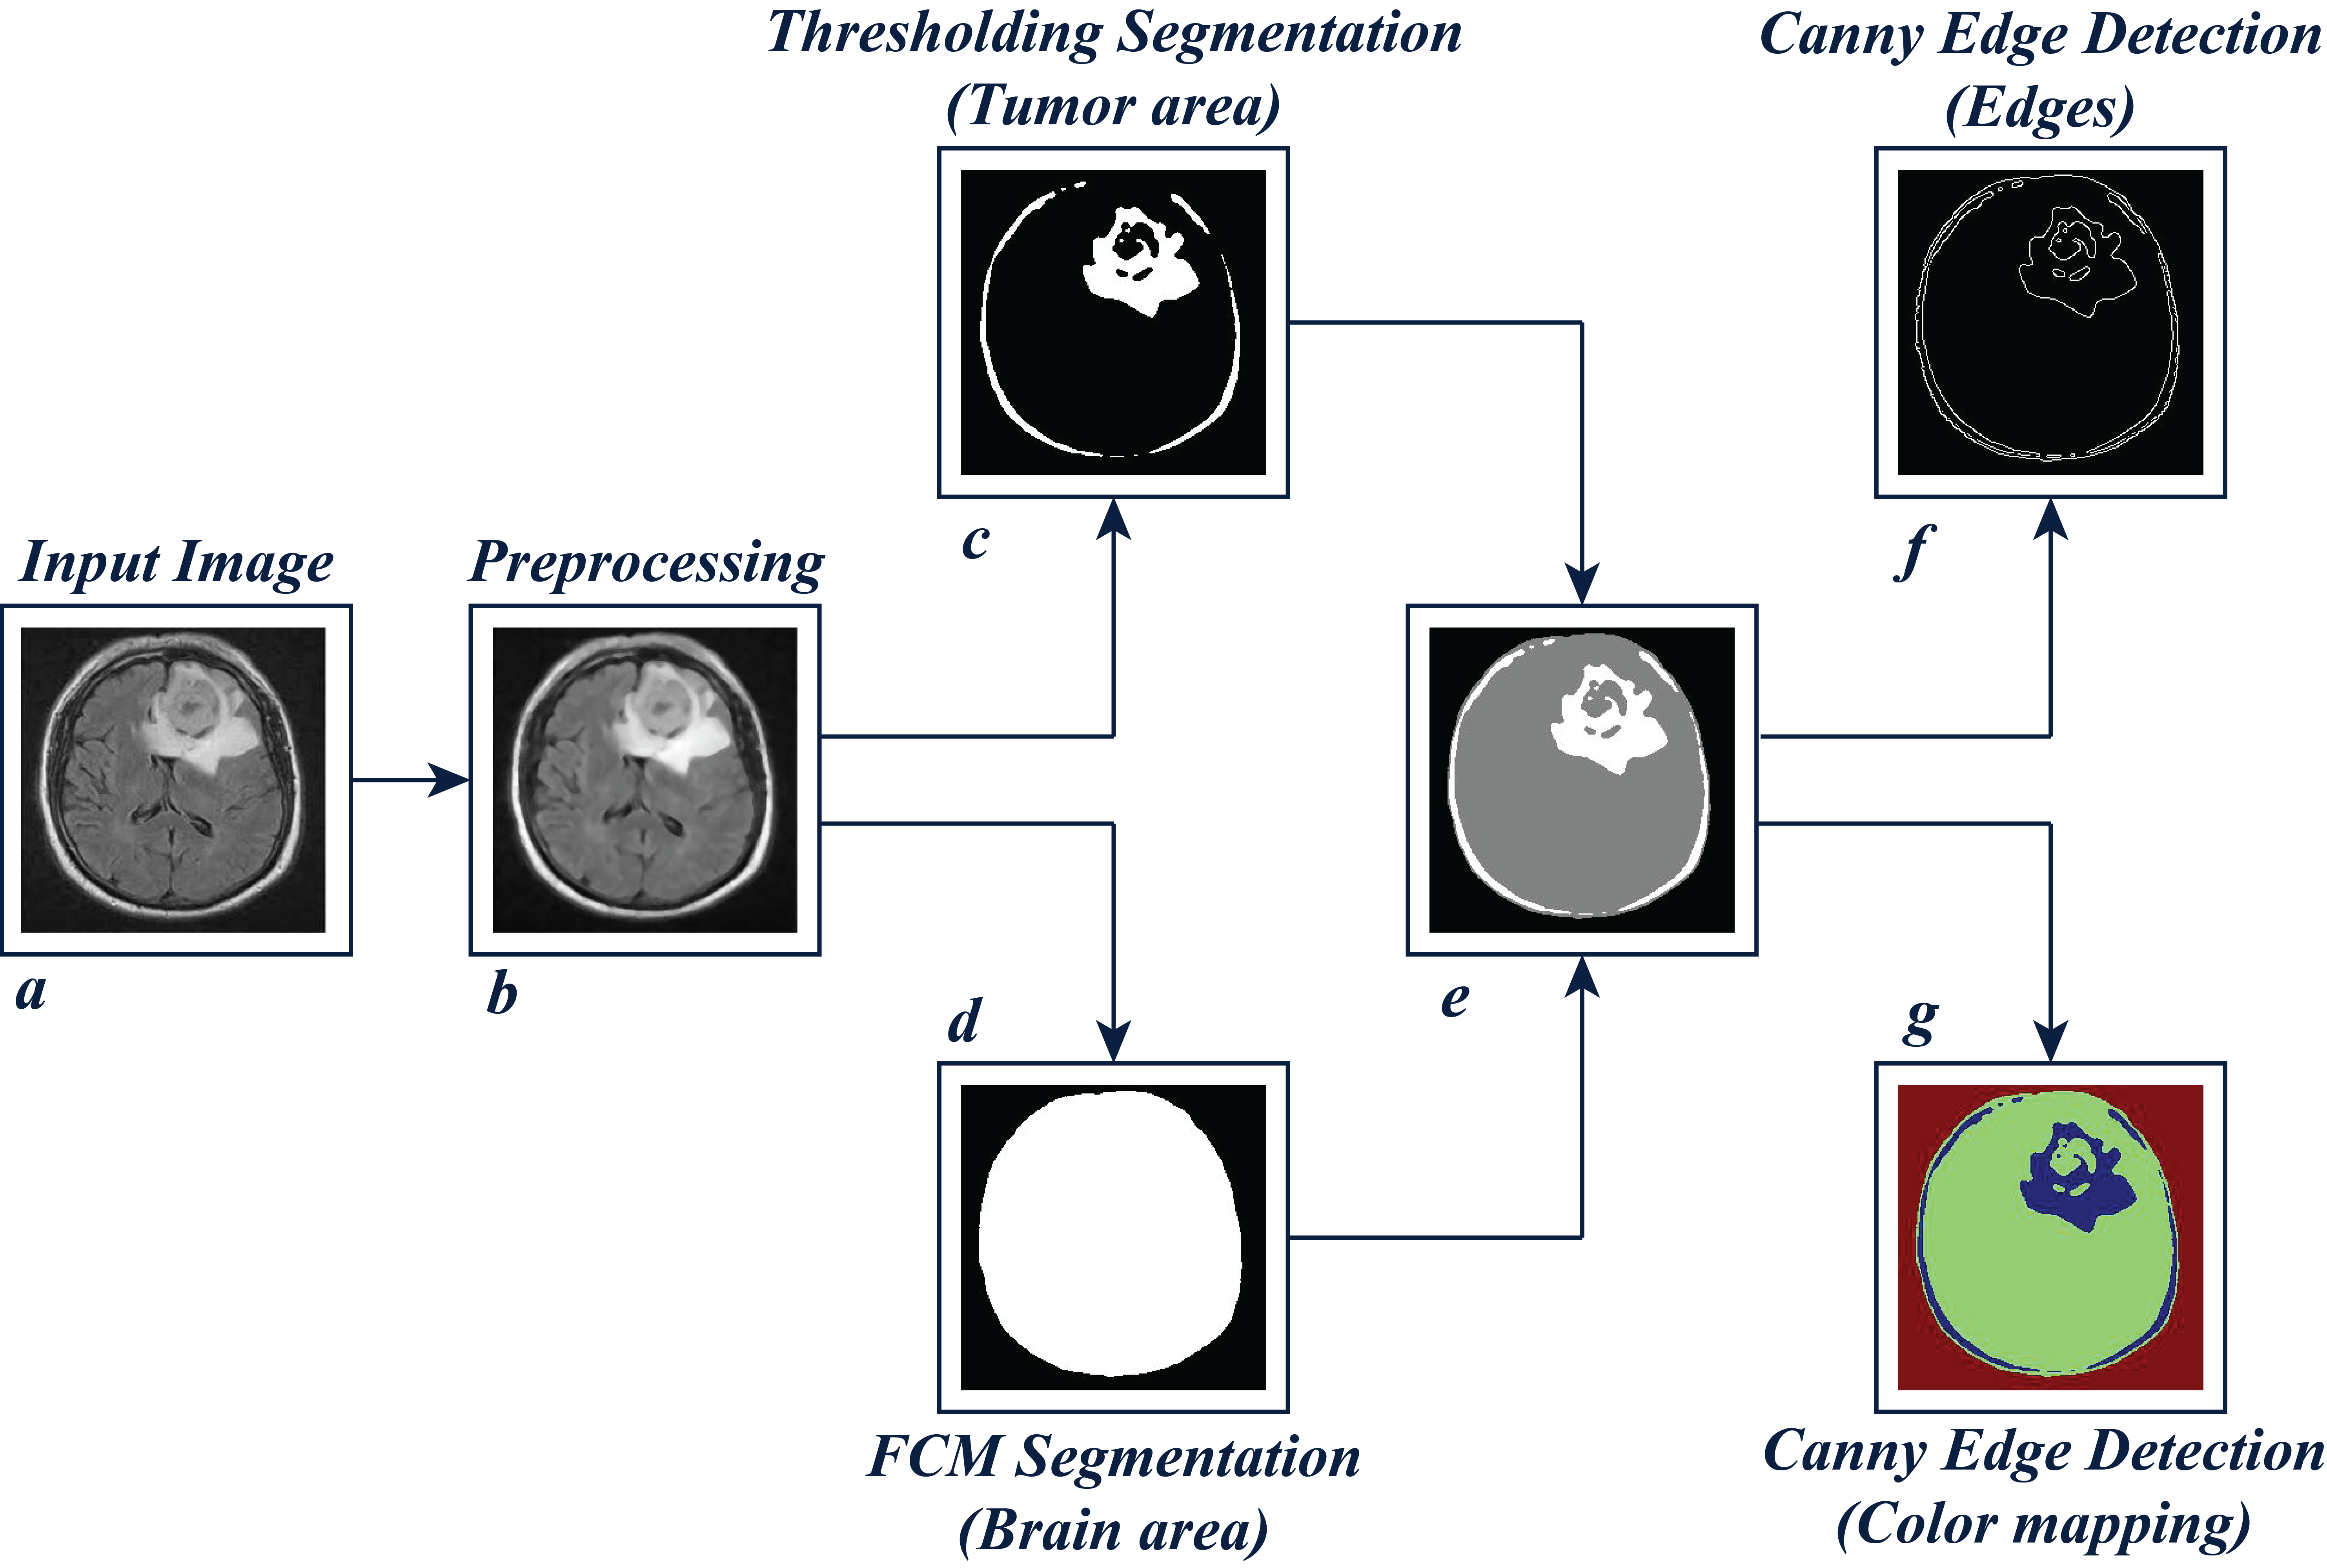
\includegraphics[width=0.9\columnwidth]{figures/Fig30.png}
	\caption{example of the system. a)input image, b)preprocessing image, c)result after thresholding, d)result after FCM clustering, e)combine both segmented images, f)final edge map, g)combined image with the color map}
	\label{fig30}
\end{figure}

This tumor segmentation system has its advantages and disadvantages. First, in cases with tumors, it has a very accurate segmentation. According to the source article, it has 97\% accuracy in detecting tumors. Also, it is simple to understand and implement due to using basic image processing and segmentation approaches. But this simplicity causes some drawbacks for this system. In MRI, tumor tissues have a similar appearance with some organs like eyes. So, usually, basic thresholding segments these normal organs as a tumor. Also, in no tumor cases, the system detects a very large brain area as the tumor.
\chapter{Conclusion}
\label{sec:conclusion}

\vspace{3cm}

\begin{adjustwidth}{70pt}{70pt}
	This research project based on learning medical image analysis with some theoretical and practical researches and activities. This project divided to 3 main stages, the first stage was introducing concepts and approaches; we covered medical imaging modalities, image processing concepts and recent improvements in segmentation and Denoising.  In the next step, we examined these concepts in practice; we provide a handy tutorial for python and OpenCV library which contains various examples for processing medical images. And, in the final step a real segmentation system was implemented. This system uses two different segmentation techniques (Fuzzy C-means and Thresholding) and then combine results. We discussed about its benefits and drawbacks. As a future work, we try to use a more complicated segmentation technique instead of simple thresholding to enhance the segmentation performance. 
	
\end{adjustwidth}

% bib
%\chapter{References}
\nocite{*}
\bibliographystyle{unsrt}
\renewcommand{\bibname}{References}

\bibliography{./Tex_files/references.bib}



\backmatter
% bibliography, glossary and index would go here.

\end{document}